\documentclass[draft,twoside,a4paper,12pt]{extarticle}

%\newcommand{\managementComputerName}{Raspberry Pi 2 Model B}

\usepackage{graphicx}
\usepackage{mathtools}
\usepackage{Format}
\usepackage{listings}
\usepackage{wrapfig}
\usepackage[table]{xcolor}

\definecolor{Gray}{gray}{0.85}

\usepackage{titlesec}
\setcounter{secnumdepth}{4}
\titleformat{\paragraph}
	{\normalfont\normalsize\bfseries}{\theparagraph}{1em}{}
\titlespacing*{\paragraph}
	{0pt}{3.25ex plus 1ex minus .2ex}{1.5ex plus .2ex}

\usepackage{listings}
\lstset{
	frame = none, 
	language=c, 
	basicstyle=\footnotesize,
	aboveskip=0.2cm,
	belowskip=-0.5cm
	%xleftmargin=\parindent,
	}

\usepackage{textcomp}
\usepackage{apacite}
\bibliographystyle{apacite}


\begin{document}
\pagenumbering{Roman}


\includepdf{Illustrationen/0-Vorspann/Titelblatt.pdf}
\input{Kapitel/0_Vorspann/0.1_Redlichkeitserklärung}
\newpage
\fontsize{12}{15}
\selectfont
\sloppy
%\begin{sffamily}
\renewcommand{\contentsname}{Inhaltsverzeichnis}
\tableofcontents
%\end{sffamily}
\newpage
\begin{comment}
	\phantomsection\addcontentsline{toc}{section}{Abbildungsverzeichnis}

	\begin{sffamily}
	\listoffigures % Abbildungsverzeichnis
	\end{sffamily}	Inhalt...
\end{comment}

\begin{comment}
	\phantomsection\addcontentsline{toc}{section}{Tabellenverzeichnis} 
	\begin{sffamily}
	\newpage
	\listoftables % Tabellenverzeichnis
	\end{sffamily} 	Inhalt...
\end{comment}

\newpage
%\begin{sffamily}
\phantomsection\addcontentsline{toc}{section}{Glossar} 
\section*{Abkürzungsverzeichnis}\label{dok:glossar}
\begin{table}[H]
	\begin{tabular}{|L{2.5cm}|L{13cm}|}

		\hline	
		\textbf{ABS} & Acrylnitril-Butadien-Styrol. Thermoplast der in der Additiven Fertigung verwendet wird.\\
		
		\hline	
		\textbf{DC} & Direct Current\\

		\hline
		\textbf{FDM} & Fused Deposition Modeling. 3D-Druckverfahren: Kunststoff wird durch eine oder mehrere Düsen extrudiert und zu Bauteillagen zusammengeführt.\\
		
		\hline
		\textbf{GND} & Ground\\
		
		\hline
		\textbf{HSLU T\&A} & Hochschule Luzern für Technik und Architektur\\ 
		
		\hline
		\textbf{KDS} & Kinetis Design Studio\\

		\hline
		\textbf{LED} & Light-emitting diode\\
		
	 	\hline
	 	\textbf{PAIND} &  Industrieprojekt (Modul der HSLU) \\ 
	 	
	 	\hline
	 	\textbf{PCB} &	Printed Circuit Board\\
				
		\hline
		\textbf{RTOS} & Real Time Operating System \\
		
		\hline
		\textbf{SoC} &	System on Chip\\
		
		\hline
		\textbf{SWD} &	Serial Wire Debug\\
		
		\hline
		\textbf{UART} &	Universal Asynchronous Receiver Transmitter\\
		
		\hline
		\textbf{USB} &	Universal Serial Bus\\		
		
		\hline
		\textbf{openSDA} & Ein Seriell- und Debugadapter, welcher in diverse NXP Entwicklungsplatformen integriert ist.\\
		
		\hline
		\textbf{HMI} & Human Machine Interface\\
				
		\hline
	\end{tabular} 
	\vspace{0.2cm}
\end{table}


\subsection*{Begrifflichkeiten}
\begin{table}[H]
	
	\begin{tabular}{|L{4.5cm}|L{11cm}|}
		\hline
		\textbf{Adhäsion} & Adhäsion blabla.\\
		
		\hline
		\textbf{Batch} & Batch blabla.\\
		
		\hline
		\textbf{BLE} & Bluetooth Low Energy: Ein unter Bluetooth 4.0 eingeführter Standard zur Datenübertragung für portable Geräte.\\
		
		\hline
		\textbf{CAD} & Computer-aided Design: Rechnerbasierte Unterstützung von konstruktiven Aufgaben in der Produktentwicklung \\
		
		\hline		
		\textbf{Demonstrator PCB} & Eine im Umfang dieses Projekts entwickelte Printplatine.\\
		
		\hline		
		\textbf{Dockingstation PCB} & Eine im Umfang dieses Projekts entwickelte Printplatine.\\
		
		\hline		
		\textbf{FRDM-Board} & In diesem Projekt ist damit spezifisch das Freedom Board KL25Z gemeint. Ein Mikrocontroller Entwicklungsboard von NXP mit einem ARM Cortex-M0+ Prozessor. \\
		
		\hline
		\textbf{Hexiwear} & Ein Mikrocontroller Entwicklungsboard von NXP mit einem ARM Cortex-M0+ mit BLE (SoC) sowie einem ARM Cortex-M4 Prozessor und diversen Sensoren.\\
		
		\hline
		\textbf{Nut} & Nut blabla\\	
			
		\hline
		\textbf{Python} & Interpretierte Programmiersprache \\
		
		\hline		
		\textbf{Raspberry} & Raspberry Pi 3 Model B: Ein kompaktes Linux basiertes Computersystem mit einem Broadcom Quad Core Prozessor, 1GB RAM und Peripherie Schnittstellen. \\	
		
		\hline
		\textbf{RGB} &  Farbraum, welcher durch das mischen von rot, blau und grün eine Farbwahrnehmung nachbildet. \\
		
		\hline
		\textbf{MDF} &  Mitteldichte Faserplatte: Ein Holzwerkstoff bestehend aus feinstzerfasertem rindenfreiem Nadelholz, welches verpresst wird.  \\		
		
		\hline
		\textbf{NemaCaps} &  Das Setzgut des Planting Robots. Von der Firma MCC Laboratoire Meiners hergestellte Kapseln in Kugelform mit Nematoden als Inhalt. \\
		
		\hline
	\end{tabular} 
	\vspace{0.2cm}
\end{table}


%\end{sffamily}
\newpage
\pagenumbering{arabic}

\newpage
\section{Abstract}
\pagenumbering{arabic}
\textit{(ygu/pro)} Der Einsatz von Fadenwürmern zur Schädlingsbekämpfung in der Landwirtschaft, sowie im Gartenbau bietet eine biologische Alternative zu konventionellen Pestiziden. Die industrielle Bestückung von Töpfen mit Kapseln, welche Fadenwürmer beinhalten, birgt im Gartenbau einen hohen personellen Aufwand. Dieser Nachteil soll durch den Einsatz eines Pflanzroboters beseitigt werden. In einer interdisziplinären Gruppe wird  ein Funktionsmuster eines Roboters entwickelt, welches die automatische Dosierung, wie auch die Platzierung von Nematoden-Kapseln in Töpfen für den Gemüse- und Zierpflanzenbau ausführt. Dabei ist der Roboter an eine halbautomatische Topfmaschine gekoppelt.
\newline

Für die Entwicklung des Funktionsmusters wurde mittels Funktionsanalyse die Aufgabe funktional abstrahiert und in lösungsneutrale Teilfunktionen zerlegt. Die Ausarbeitung von drei Lösungskonzepten erfolgte durch die funktionsbezogene Variation von Teillösungen und einer Konzeptauswahl mittels morphologischem Kasten. Für eine verbesserte Einschätzung der Machbarkeit wurden kritische Teilfunktionen einem praktischen Funktionsnachweis unterzogen. Als Resultat der Nutzwertanalyse wurde eines der drei Konzepte für die Umsetzung ausgewählt.
\newline

Während der praktischen Umsetzung des Konzepts erfolgte die Entwicklung der Konstruktion, Software sowie der Elektronik in vermehrt fachspezifischer Arbeit. Die entwickelten Komponenten wurden hergestellt und als Gesamtsystem montiert. Abschliessend wurden Funktionstest an den einzelnen Einheiten durchgeführt.
\newline

Anhand des Funktionsmusters konnte aufgezeigt werden, dass eine industrielle Bestückung von NemaCaps realisitisch ist. Die Vereinzelung der Kapseln sowie die Konfiguration der Setzeinheit konnte durch das Funktionsmuster erfüllt werden. Weiter bleibt das Zusammenspiel aller Funktionen zu überprüfen, da eine umfassende Überprüfung innerhalb des gesetzten Zeitrahmen nicht realisierbar war.
\newline

Die gewonnenen Erkenntnisse aus den Funktionstests lassen vermuten, dass durch gezielte Anpassungen an der Setzeinheit die gestellte Aufgabe mit dem gewählten Konzept möglich ist. Für die abschliessende Umsetzung werden konkrete Massnahmen genannt.

\newpage
The application of nematodes for pest control in agriculture and gardening offers a biological alternative to conventional pesticides. The industrial assemby of pots with capsules which contain nematodes implies higher human resources in gardening than usual. This disadvantage is to be resolved by the application of a robot. In an interdisciplinary team, the development of a functional prototype of such a robot is to be undertaken which doses and places nematode-capsules in pots automatically. The pots are used for vegetable gardening and ornamental plants. The functional prototype is linked with a semi-automatic potting machine.
\newline

The development of this functional prototype was abstracted by a functional analysis. Furthermore an objective observation was undertaken and the main-function of the prototype was split into several sub-functions. Based on the functional analysis, an elaboration of three concepts was done by using creativity techniques and a morphological box. In order to support the assessment of those concepts, critical functions were tested. One of those concepts was chosen to be realised as a consequence of the utility analysis.
\newline

During the practial implementation of the chosen concept such as the design of the electronics, the software and the whole mechanical setup was carried out in mainly subject-specific tasks. The developed components were assembled and merged to a system. finally, the assembled components were undergone extensive testing procedures.
\newline

As conclusion the assembled functional prototype was shown to be able of handling NemaCaps. The separation of NemaCaps and configuration of the planting unit was tested successfully. An extensive examination of the  interaction between all functions could not be verified yet due to the lack of time.
\newline

The gained findings from testing the functional prototype lead to the supposition that an industrial assembly of NemaCaps with the chosen concept is likely. In order to finish the implementation thoroughly, specific measures are listed.

\newpage
\section{Projektmanagement}
\subsection{Methodik}
\label{methodik}
\textit{(ygu)} Diese Bachelorarbeit befasst sich mit systematischen Produktentwicklung eines Pflanzroboters. Das systematische Vorgehen orientiert sich  an der VDI-Richtlinie 2221, welche in folgende Phasen unterteilt wird \cite{naefe}:

\begin{itemize}
	\item \textbf{Phase I:} Planen und klären der Aufgabe durch informative Festlegung
	
	\item \textbf{Phase II:} Konzipieren durch prinzipielle Festlegung
	
	\item \textbf{Phase III:} Gestalterische Festlegung der angestrebten Lösung
	
	\item \textbf{Phase IV:} Ausarbeiten, Erstellung der erforderlichen Unterlagen
	
\end{itemize}

Phase I stellt der eigentliche Entwurf des Systems dar. Gemäss VDI-Richtlinie 2221 beinhaltet diese Phase im Wesentlichen das Klären der Aufgabenstellung sowie die Ermittlung von Funktionen \cite{vdi2221}. Für die Klärung der Aufgabenstellung wurde in Zusammenarbeit mit dem Auftraggeber (MCC Laboratoire Meiners GmbH) ein Pflichtenheft ausgearbeitet. Darin sind alle relevanten Eigenschaften und Anforderungen an das Produkt formuliert. Dieses Dokument dient als Grundlage für die weitere Entwicklung des Produktes und grenzt die Aufgabenstellung der Hochschule Luzern weiter ein. Der zweite Teil von Phase I, die Ermittlung der Funktionen, gestaltet sich wie folgt \cite{pahl}:

\begin{itemize}
	\item \textbf{Hauptfunktion:} Aufbauend auf der Aufgabenstellung sowie dem erarbeitetem Pflichtenheft, ergibt sich die Hauptfunktion des Pflanzroboters.
	
	\item \textbf{Aufgliederung in Teilfunktionen:} Die Hauptfunktion wird mittels Funktionsanalyse in verschiedene Teilfunktionen unterteilt. So wird die Aufgabenstellung abstrahiert und rein funktional betrachtet. Dadurch wird eine möglichst lösungsneutrale Betrachtung des Problems gewährleistet. 
	
	\item \textbf{Funktionsbezogene Variation:} Für die ausgearbeiteten Teillösungen werden mögliche Lösungsansätze erarbeitet. Dafür wurden Kreativitätstechniken verwendet, um eine Vielzahl von Lösungsansätzen für jede Teilfunktion zu generieren.

\end{itemize}

Nach  VDI-Richtlinie 2221 befasst sich Phase II mit der Ausarbeitung eines Konzepts. Dabei werden die generierten Ideen aus der funktionsbezogenen Variation aufgegriffen und zu einem Konzept ausgearbeitet. Aufgebaut ist diese Phase wie folgt \cite{vdi2221}:

\begin{itemize}
	\item \textbf{Suchen nach Lösungsprinzipien:} Konkrete Teillösungen der funktionsbezogenen Variation werden zu einer Gesamtlösung zusammengesetzt, wodurch ein Gesamtkonzept entsteht. Dafür wurden alle Teillösungen in einem morphologischen Kasten aufgelistet und in einem ersten Schritt fünf Konzepte ausgearbeitet. In einem weiteren Schritt wurden die Auswahl auf drei Konzepte eingegrenzt (Erklärung wie dies geschah nötig?).
	
	\item \textbf{Gliedern in realisierbare Module:} Die Konzepte wurden durch die Gestaltung von Konzeptskizzen visualisiert und zum ersten Mal als gesamtes Konzept dargestellt. 
	
	\item \textbf{Funktionsnachweis kritischer Funktionen:} Ergänzend zur VDI-Richtlinie 2221 wurde ein Funktionsnachweis von kritischen Funktionen erbracht. Dabei wurden einfach aufgebaute, praktische Versuche der erarbeiteten Teillösung realisiert, um die Funktionalität zu validieren (überprüfen?).
	
	\item \textbf{Bewertung:} Hinzukommend zur VDI-Richtlinie 2221 wurden die ausgearbeiteten Konzepte einer objektiven Bewertung unterzogen. Dabei wurde eine Nutzwertanalyse durchgeführt \cite{pahl}:
	\begin{itemize}
		\item Fünf Ziele wurden definiert, welche funktionale sowie auch wirtschaftliche Anforderungen beinhalten. Für jedes Ziel wurde eine Gewichtung vorgenommen, wobei in der vorliegenden Arbeit die Funktionserfüllung höher gewichtet wurde als der Kostenaspekt.
		
		\item Jedes der ausgearbeiteten Konzepte wurde nach VDI-Richtlinie 2225 mit einer Wertskala von 0 bis 4 (von unbefriedigend bis ideal) bewertet \cite{vdi2225}. Dabei wurden auch die gewonnenen Erkenntnisse aus dem Funktionsnachweis miteinbezogen. Wichtig ist dabei, dass die Beurteilung völlig objektiv erfolgt.
	\end{itemize}	
	
	\item \textbf{Entscheid:} Die Nutzwertanalyse wird ausgewertet und das Konzept mit dem höchsten Nutzwert ausgewählt. Dieses kommt nun in Phase III zur Umsetzung. 
\end{itemize}

In Phase III wird das ausgewählte Konzept umgesetzt. Dabei wird in dieser Phase vermehrt fachspezifisch gearbeitet. Aufgebaut ist die Umsetzungsphase folgendermassen:
\begin{itemize}
	\item \textbf{Gestalten der Module:} Die Teillösungen des Konzepts werden konkret in Baugruppen realisiert. Dies geschieht auf allen technischen Ebenen; sei es Software, PCB-Design oder Konstruktion. Zuerst wurde hierfür eine Evaluation von möglichen Komponenten durchgeführt. Wenn nötig, wurden Berechnungen zur Auswahl der Komponenten gemacht. Dabei ist eine stetige Absprache zwischen Elektrotechnik und Maschinentechnik essentiell, um Missverständnisse und Fehler zu vermeiden.
	
	\item \textbf{Gestalten des Produktes:} Dies beinhaltet das konstruktive Zusammenführen aller Baugruppen zu einem Produkt. Fertigungsunterlagen für die verwendeten Fertigungsverfahren wurden erstellt und in Auftrag gegeben. Parallel dazu wurde die Bestellung der Komponenten ausgelöst und Offerten von Herstellern eingeholt. 
\end{itemize}

Die Phase IV umfasst die Ausarbeitung des Produktes. Dabei weicht die vorliegende Bachelorarbeit von der VDI-Richtlinie 2221 ab, da sich diese Arbeit mit der Entwicklung eines Funktionsmusters beschäftigt (und nicht eines Serienproduktes).
\newline
Die Ausarbeitung in dieser Phase legt den Fokus auf die Montage und Inbetriebnahme des Funktionsmusters. Die einzelnen Baugruppen werden an Funktionstests unterzogen dadurch auf ihre Funktionalität geprüft. Sind alle Baugruppen funktionsfähig, kann das Gesamtsystem getestet werden.
\newline
Während der gesamten Bachelorarbeit werden alle relevanten Schritte und Überlegungen (methodischer sowie technischer Art) dokumentiert und in einem Bericht festgehalten.
\subsection{Projektplan}
\textit{(ygu)} Vorgängig wurde für beide Fachrichtungen ein Projektplan ausgearbeitet. Dabei wurden die wichtigsten Arbeitsschritte in sogenannte Work-Packages gegliedert und orientiert an der Methodik aus Kapitel \ref{methodik} geordnet. Nun wurde der Zeitbedarf für jedes Work-Package eingeplant, wobei eine Auflösung auf einen Tag als angemessen erschien. Ergänzt wurde der Projektplan mit:

\begin{itemize}
	\item \textbf{Meilensteine}, welche den Abschluss wichtiger Phasen markieren.
	
	\item \textbf{Besprechungen} mit dem betreuenden Dozenten.
	
	\item \textbf{Reservezeit} für Work-Packages die zeitlich schwer kalkulierbar sind. Auch nimmt die Dauer der eingeplanten Reservezeit im Verlauf des Semesters zu.
	
	\item \textbf{Notizen} relevanter Ereignisse.
\end{itemize}

Während dem Verlauf dieser Bachelorarbeit wurde die tatsächlich benötigte Zeit erfasst. Dies ermöglicht einen Vergleich zwischen Planung sowie praktischer Umsetzung des Projekts. Dieser Vergleich wird im Kapitel \ref{projektplan} gemacht. Die Projektpläne beider Fachrichtungen sind im Anhang ersichtlich. 
\subsection{Risikomanagement}
\subsection{Finanzierung}
\textit{(ygu)} Die Finanzierung der vorliegenden Bachelorarbeit obliegt vollständig MCC Laboratoire Meiners GmbH als Industriepartner des Projekts. Im Einverständnis des Partners wurde vereinbart, dass für grössere Ausgaben Kostenvoranschläge erstellt werden. Bevor diese Ausgaben getätigt werden, sind sie durch Jean-Antoine Meiners zu genehmigen. Einmalige Ausgaben unter 100 CHF dürfen ohne Genehmigung getätigt werden. Sämtliche Kostenvoranschläge sind im Anhang aufgelistet. Auch wird im Kapitel \ref{finanzierung} eine Bilanz aller Ausgaben gemacht. 


\newpage
\section{Einleitung}
\begin{wrapfigure}[16]{r}{8.5cm}
	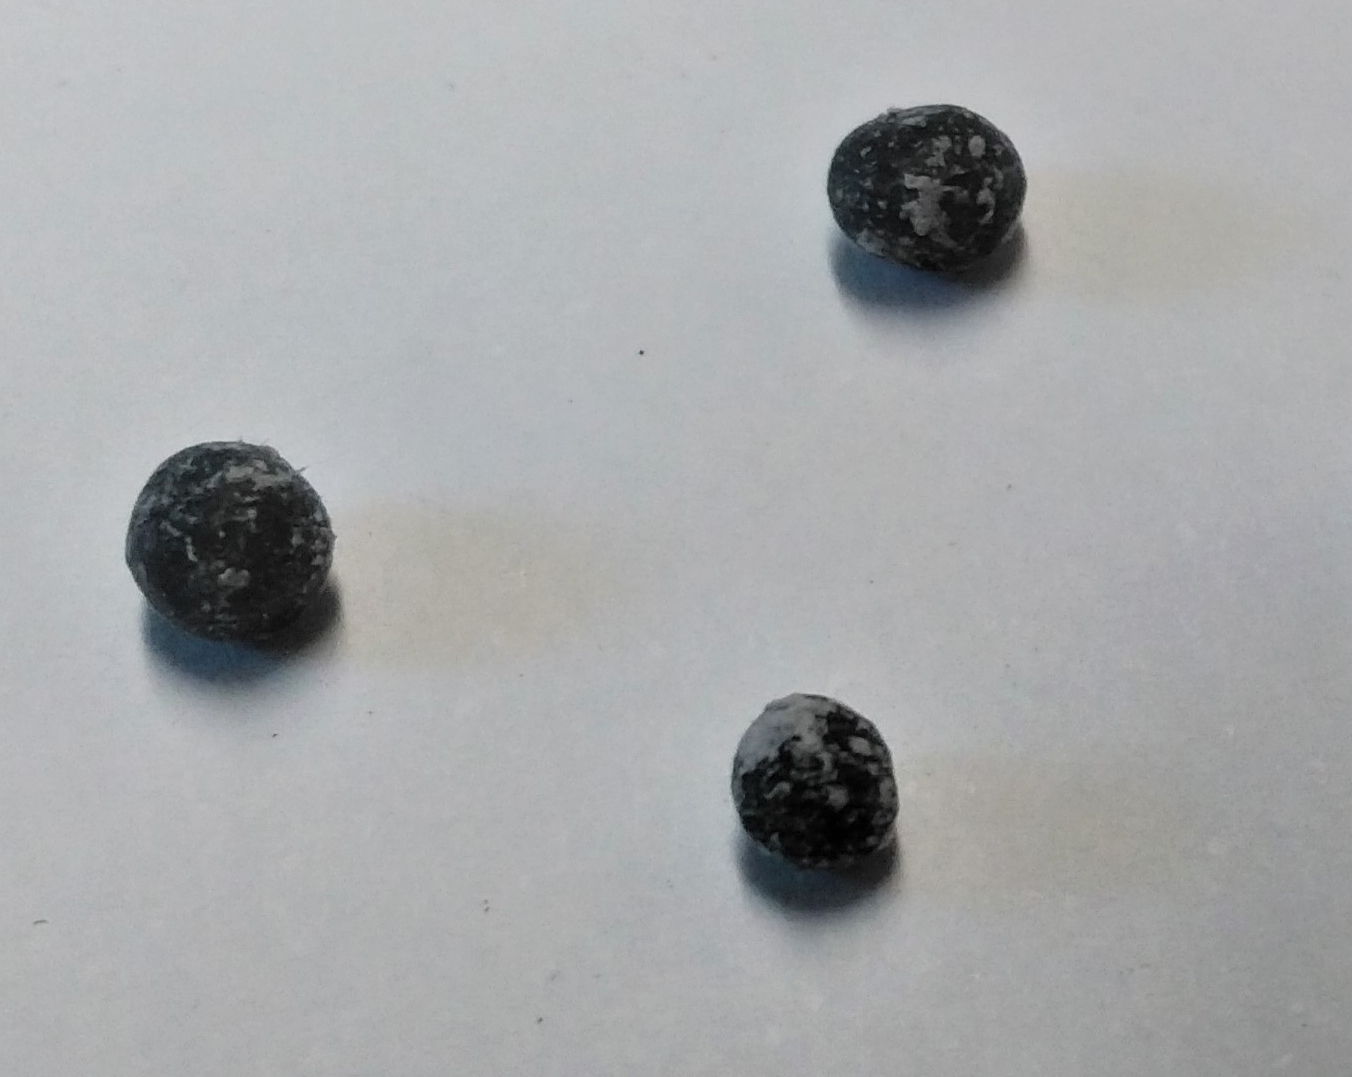
\includegraphics[scale=0.11]{Illustrationen/3-Einleitung/nemacaps.jpg}
	\caption{NemaCaps}
	\label{fig:nemacaps}
\end{wrapfigure}
Die Firma MCC Laboratoire Meiners GmbH ist in der Herstellung von Mikroverkapselungen tätig. Neben der Pharma- und Kosmetikbranche werden Mikroverkapselungen auch in der Landwirtschaft eingesetzt. Für diese Branche entwickelt MCC Laboratoire Meiners GmbH Kapseln, sogenannte NemaCaps, welche in der biologischen Schädlingsbekämpfung eingesetzt werden. Ein NemaCap beinhaltet mehrere tausend Fadenwürmer (Nematoden). Neben Nematoden ist der Kapsel ein Schlafmittel beigemischt, sodass die Fadenwürmer schlafend gestellt sind. 
\newline
NemaCaps werden im Erdreich eingesetzt. Im Wurzelbereich der zu schützenden Pflanze werden diese platziert. Durch das Begiessen der Pflanze oder Regenfall wird das Schlafmittel verdünnt und die Nematoden werden aktiv. Die Hülle der Kapseln besteht aus \textbf{\textit{XYZ}} welches elastische Eigenschaften besitzt. Dies ist Voraussetzung, dass die Nematoden nach dem Aufwachen die Kapsel durchbrechen können.\newline
In ihrer natürlichen Umgebung angelangt stossen die Fadenwürmer nun zufällig auf Larven von Schädlingen. Gemäss dem Nationalen Forschungsprogramm 68 [nachfolgend NFP 68]\cite{nfp} dringen die Nematoden durch die Körperöffnungen der Larven ein (Siehe Abb.  \ref{fig:zyklus_Nematoden}, Punkt 3). im Körper der Larve angelangt, setzen die Fadenwürmer dort Bakterien frei (Punkt 1 in Abb.  \ref{fig:zyklus_Nematoden}). Durch die rapide Vermehrung dieser Mikroben wird die Larve abgetötet. Im Innern der Larve vermehren sich nun die Nematoden bis diese komplett aufgezehrt ist \cite{nematoden}. Anschliessend verlassen die Nematoden den Kadaver und befallen weitere Larven. So beginnt der Kreislauf von Neuem (Punkt 2 in Abb.  \ref{fig:zyklus_Nematoden}).
\newline

\begin{wrapfigure}[10]{r}{7cm}
	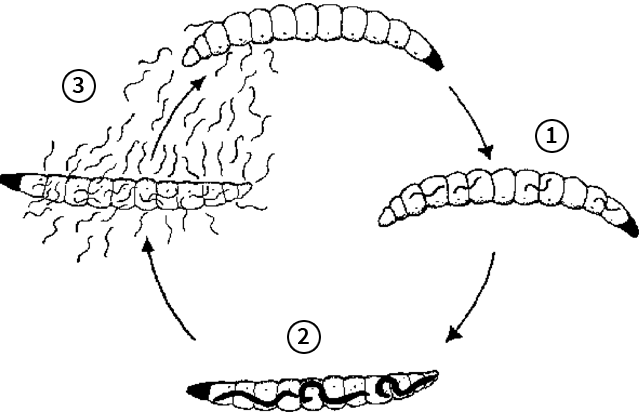
\includegraphics[scale=0.4]{Illustrationen/3-Einleitung/zyklus_nematoden.png}
\caption{Bekämpfung einer Larve durch Nematoden}
\label{fig:zyklus_Nematoden}
\end{wrapfigure}

	
Nematoden bieten speziell in der Bekämpfung gegen Wurzelschädlinge eine wirksame Alternative zu Pestiziden an. Pestizide können im Wurzelbereich weniger gezielt eingesetzt werden \cite{nfp}. Die Überlegenheit der Nematoden (im Wurzelbereich?) will man mit NemaCaps nutzen. Durch die Kapselung ist eine gezielte Platzierung sowie Dosierung von Nematoden möglich. Ein weiterer Vorteil der Kapselung ist die verbesserte Handhabung. Die einfache Lagerung sowie Transport von Fadenwürmer wird möglich.  Zusätzlich verlängert die Verwendung von Schlafmittel die Haltbarkeit der Nematoden. Diese Vorteile unterstreichen das Potential von NemaCaps, der biologischen Alternative von Pestiziden.

\newpage
\section{Einleitung}
Die Firma MCC Laboratoire Meiners GmbH ist in der Herstellung von Mikroverkapselungen tätig. Neben der Pharma- und Kosmetikbranche werden Mikroverkapselungen auch in der Landwirtschaft eingesetzt. Für diese Branche entwickelt MCC Laboratoire Meiners GmbH Kapseln, sogenannte NemaCaps, welche in der biologischen Schädlingsbekämpfung eingesetzt werden. Ein NemaCap beinhaltet mehrere tausend Fadenwürmer (Nematoden). Der Kapsel ist ein Schlafmittel beigemischt, sodass die Fadenwürmer schlafend gestellt sind. 
\begin{figure}[H]
	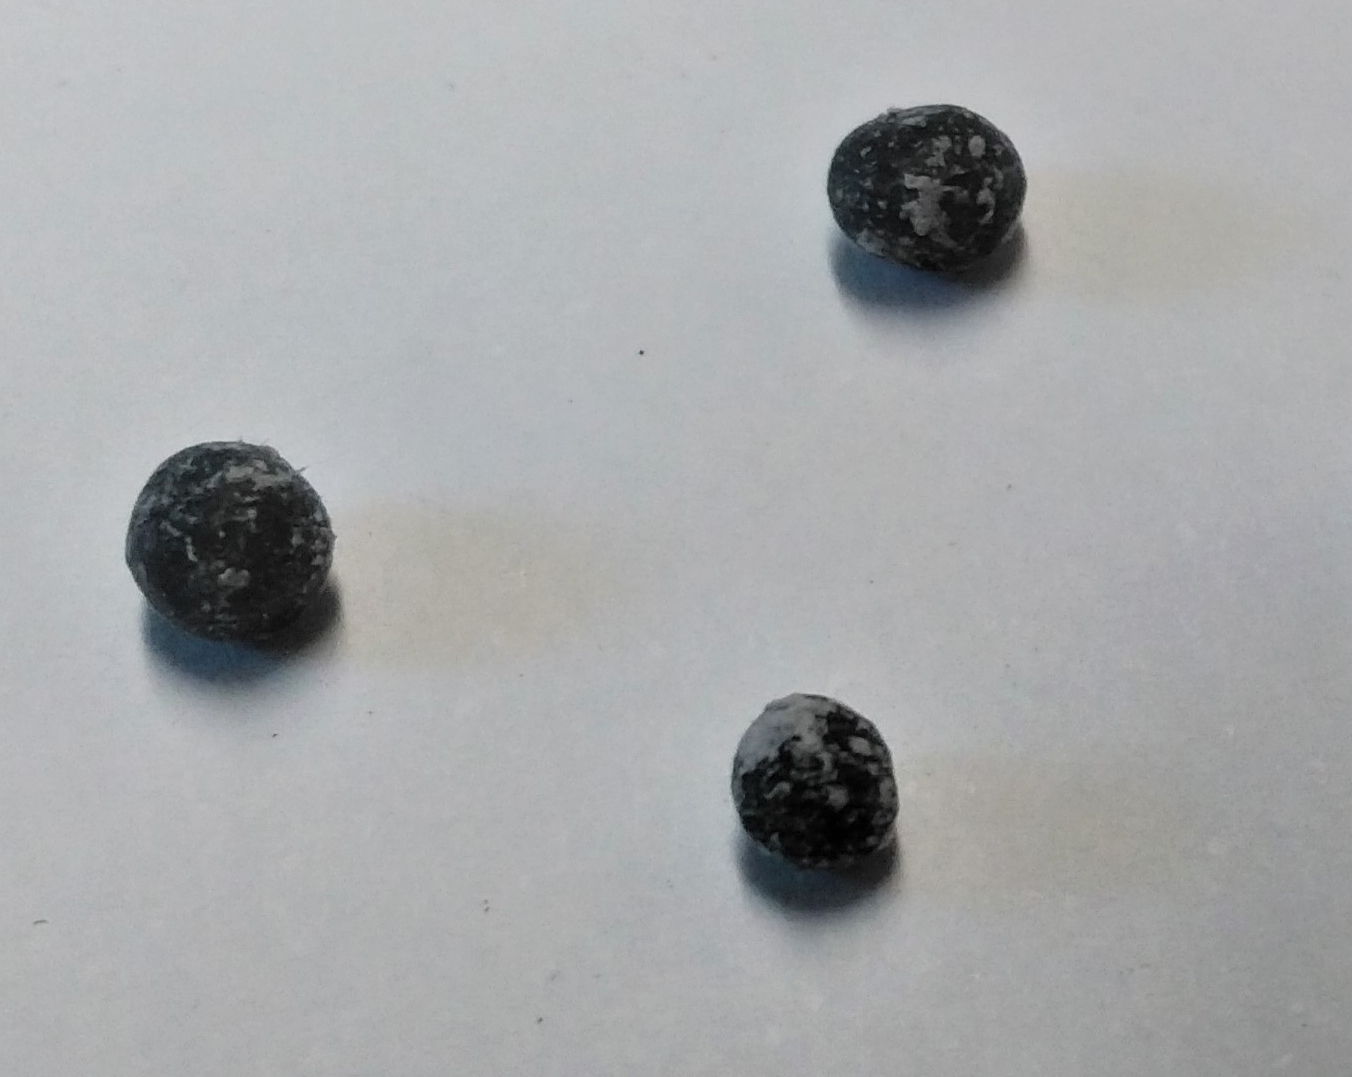
\includegraphics[width=1\textwidth]{Illustrationen/3-Einleitung/nemacaps.jpg}
	\caption{NemaCaps}
	\label{fig:nemacaps}
\end{figure}
NemaCaps werden im Erdreich eingesetzt. Im Wurzelbereich der zu schützenden Pflanze werden diese platziert. Durch das Begiessen der Pflanze oder Regenfall wird das Schlafmittel verdünnt und die Nematoden werden aktiv. Die Hülle der Kapseln besteht aus \textbf{\textit{XYZ}} welches elastische Eigenschaften besitzt. Dies ist Voraussetzung, dass die Nematoden nach dem Aufwachen die Kapsel durchbrechen können.\newline
In ihrer natürlichen Umgebung angelangt stossen die Fadenwürmer nun zufällig auf Larven von Schädlingen. Gemäss dem Nationalen Forschungsprogramm 68 [nachfolgend NFP 68] (2015) dringen die Nematoden durch die Körperöffnungen der Larven ein (Siehe Abb.  \ref{fig:zyklus_Nematoden}, Punkt 3). im Körper der Larve angelangt, setzen die Fadenwürmer dort Bakterien frei (Punkt 1 in Abb.  \ref{fig:zyklus_Nematoden}). Durch die rapide Vermehrung dieser Mikroben wird die Larve abgetötet. Nach Leillinger und Löckener (2012) vermehren sich die Nematoden im Innern der Larve bis diese komplett aufgezehrt ist. Nun verlassen die Nematoden den Kadaver und befallen weitere Larven. So beginnt der Kreislauf erneut von vorne (Punkt 2 in Abb.  \ref{fig:zyklus_Nematoden}).\newline
\begin{figure}[H]
	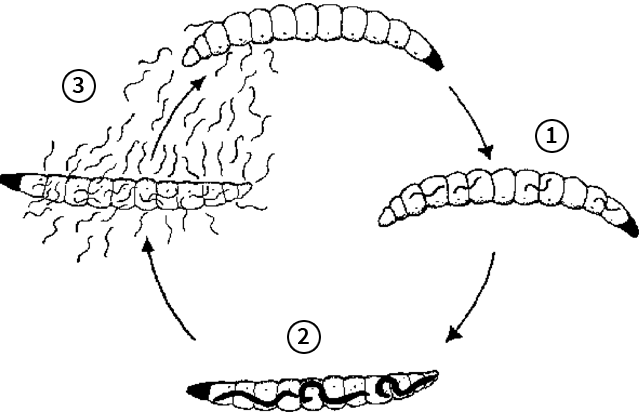
\includegraphics[width=1\textwidth]{Illustrationen/3-Einleitung/zyklus_nematoden.png}
	\caption{Bekämpfung einer Larve durch Nematoden}
	\label{fig:zyklus_Nematoden}
\end{figure}
	
Nach dem NFP 68 (2015) bieten Nematoden speziell in der Bekämpfung gegen Wurzelschädlinge eine wirksame und sichere Alternative zu Pestiziden an, welche im Wurzelbereich weniger gezielt eingesetzt werden können. Dadurch werden die Vorteile der NemaCaps gegenüber von Pestiziden deutlich. Nematoden können im Wurzelbereich gezielt platziert sowie dosiert werden. Ein Vorteil der Kapselung ist die verbesserte Handhabung. Die einfache Lagerung sowie Transport von Fadenwürmer wird möglich.  Zusätzlich wird durch die Verwendung des Schlafmittels die Haltbarkeit der Nematoden verlängert. Diese Vorteile unterstreichen das Potential von NemaCaps, der biologischen Alternative von Pestiziden.

\subsection{Ausgangslage}
Der Einsatz von Nematoden ist im Gartenbau verbreitet. Konventionell werden Nematoden gemäss Birchmeier (\textbf{\textit{2017}}) in Wasser aufgelöst und durch ein Dosiergerät oder eine Spritzkanne in Pflanzennähe aufgetragen. Solche Produkte werden jedoch erst bei erhöhtem Befall von Schädlingen eingesetzt. Der Ansatz der Firma MCC Laboratoire Meiners GmbH ist jedoch ein Anderer. Präventiv möchten Sie Nematoden in Topfpflanzen einsetzen. Im Detailhandel sollen so Topfpflanzen - bereits bestückt mit NemaCaps - im Verkauf angeboten werden.
\newline
Die industrielle Anwendung von NemaCaps birgt bei manueller Bestückung von Töpfen einen hohen personellen Aufwand. 
\subsection{Aufgabenstellung}
MCC Laboratoire Meiners GmbH möchte ihr Produkt (NemaCaps) während der halbautomatischen Bestückung von Topfpflanzen in den Töpfen platzieren. Nach der Beschüttung der Erde (Punkt 2 in Abbildung \ref{fig:schema_topfmaschine}) sollen NemaCaps im Wurzelbereich der Pflanze platziert werden. Die manuelle Bestückung von NemaCaps würde einen zusätzlichen personellen Aufwand bedeuten. Ob Gartenbauunternehmen bereit sind diesen aufzuwenden, darf hinterfragt werden. Um den Einsatz von NemaCaps lukrativer zu gestalten, möchte MCC Laboratoire Meiners GmbH ein automatisiertes System (besser Roboter?) entwickeln, welcher die Bestückung der NemaCaps ausführt (übernimmt?). Dabei soll dieses System auch in der Lage sein, verschiedene Topfgrössen zu handhaben.
\newline

Diese Bachelorarbeit befasst sich mit der Entwicklung eines Funktionsmusters, welche die automatische Bestückung von NemaCaps an einer Topfmaschine übernimmt. Dieses Funktionsmuster soll eine greifbare Vorstellung vermitteln, wie die industrielle Implementierung dieser Automatisationsaufgabe aussehen kann. 
\newline 

Die Aufgabenstellung beinhaltet:
\begin{itemize}
	\item \textbf{Ausarbeitung eines Pflichtenhefts:} Am Anfang vom Entwicklungsprozess steht eine genaue Analyse der Aufgabenstellung. In Zusammenarbeit mit MCC Laboratoire Meiners GmbH soll der Umfang der Bachelorarbeit abgegrenzt werden. Produkteigenschaften, Anforderungen an das Funktionsmuster und Randbedingungen (gegeben durch Topfmaschine, Töpfe und Topferde) stehen dabei im Fokus. Am Ende dieser Phase soll ein detailliertes Pflichtenheft entstehen.
	 
	\item \textbf{Konzeptausarbeitung und Entscheid:} Auf das Pflichtenheft folgt die interdisziplinäre Ausarbeitung von Lösungsvarianten. Durch eine sorgfältige Auslegung aller Vor- und Nachteile der ausgearbeiteten Lösungsvarianten soll die Beste Lösungsvariante ausgeweählt werden. Wichtig ist dabei, dass durch die funktionelle Abstraktion der Aufgabe eine lösungsneutrale Betrachtung möglich wird. Erst dies schafft die Grundlage für einen kreativen Lösungsfindungsprozess und gewährleistet eine volle Auschöpfung des Potenzials dieser Phase. Am Ende dieser Phase, und nach einer objektiven Beurteilung aller Lösungsvarianten, soll ein Entscheid stehen, welches der ausgewählten Lösungsvarianten umgesetzt wird.
	
	\item \textbf{Funktionsnachweis krtischer Funktionen:} Teillösungen, die als kritisch erachtet werden, sind einem praktischen Funktionsnachweis zu unterziehen. Die Erkenntnisse des Funktionsnachweises sollen unterstützend in die Beurteilung der Lösungskonzepte einfliessen und den Entscheid stützen.
	
	\item \textbf{Realisation eines Funktionsmusters:} In der Implementationphase soll das ausgearbeitete Konzept als Funktionsmuster realisiert werden. In dieser Phase werden fachspezifisch die einzelnen Komponenten hergestellt und getestet. (Mehr nötig?)
	
	\item \textbf{Erstellung eines Projektplans:} Die gewünschte Realisation eines Funktionsmusters erfordert einen klar definierten Zeitplan. Darin sollen auch Lieferfristen und der erforderliche Zeitbedarf von Fertigungsverfahren mitberücksichtigt werden. Auch sollen Reservezeiten eingeplant werden, falls allfällige Verzögerungen eintretten. Optional (Idealerweise?) wird dieser Projektplan von einer Risikoanalyse begleitet (unterstützt?).
	
	\item \textbf{Dokumentation:} Eine umfassende schriftliche Dokumentation über die methodische Vorgehensweise sowie aller relevanten technischen Überlegungen ist zu verfassen. 
	
\end{itemize}

\newpage
\section{Entwurf}
\textit{(pro)} Dieses Kapitel soll einen Überblick über die Rahmenbedingungen sowie die Anforderungen an den Planting Robot bieten. Ausführlichen Angaben zu diesen Themen sind im Pflichtenheft (siehe Anhang) formuliert. Basierend auf dem Pflichtenheft wurde ein abstrakter Entwurf des Planting Robots in Form einer Funktionsanalyse erstellt. Der Inhalt dieses Kapitels resultiert aus der Zusammenarbeit mit der Firma MCC Laboratoire Meiners, dem Topfmaschinenhersteller Leidolt Maschinenbau sowie den betreuenden Dozenten dieses Projektes.

\subsection{Rahmenbedingungen}
Die in diesem Unterkapitel beschriebenen Rahmenbedingungen sollen die Aufgabenstellung präzisieren und auf den Umgang mit den in diesem Projekt verwendeten Materialien aus dem Agrar-Bereich sensibilisieren.

\subsubsection{NemaCaps}
Die geometrischen Abmessungen der NemaCaps sind entscheidend, da sie während des Setzprozesses vereinzelt und transportiert werden müssen. Die Abmessungen der NemaCaps wurden deshalb vom Hersteller MCC Laboratoire Meiners mit 3mm Durchmesser und einer Toleranz von +0.6mm spezifiziert. Von Bedeutung ist ausserdem das Alter und die Lagerung der Nemacaps. Sie müssen in einem geschlossenen Gefäss, unter Beigabe eines hygrophoben Pulvers bei unter 7°C gelagert werden. Dabei sollten sie zur Zeit der Verwendung nicht älter als 4 Wochen sein. NemaCaps welche längere Zeit der Umgebungsluft ausgesetzt waren, schrumpfen um ein Vielfaches ihrer ursprünglichen Grösse.

\begin{figure}[H]
	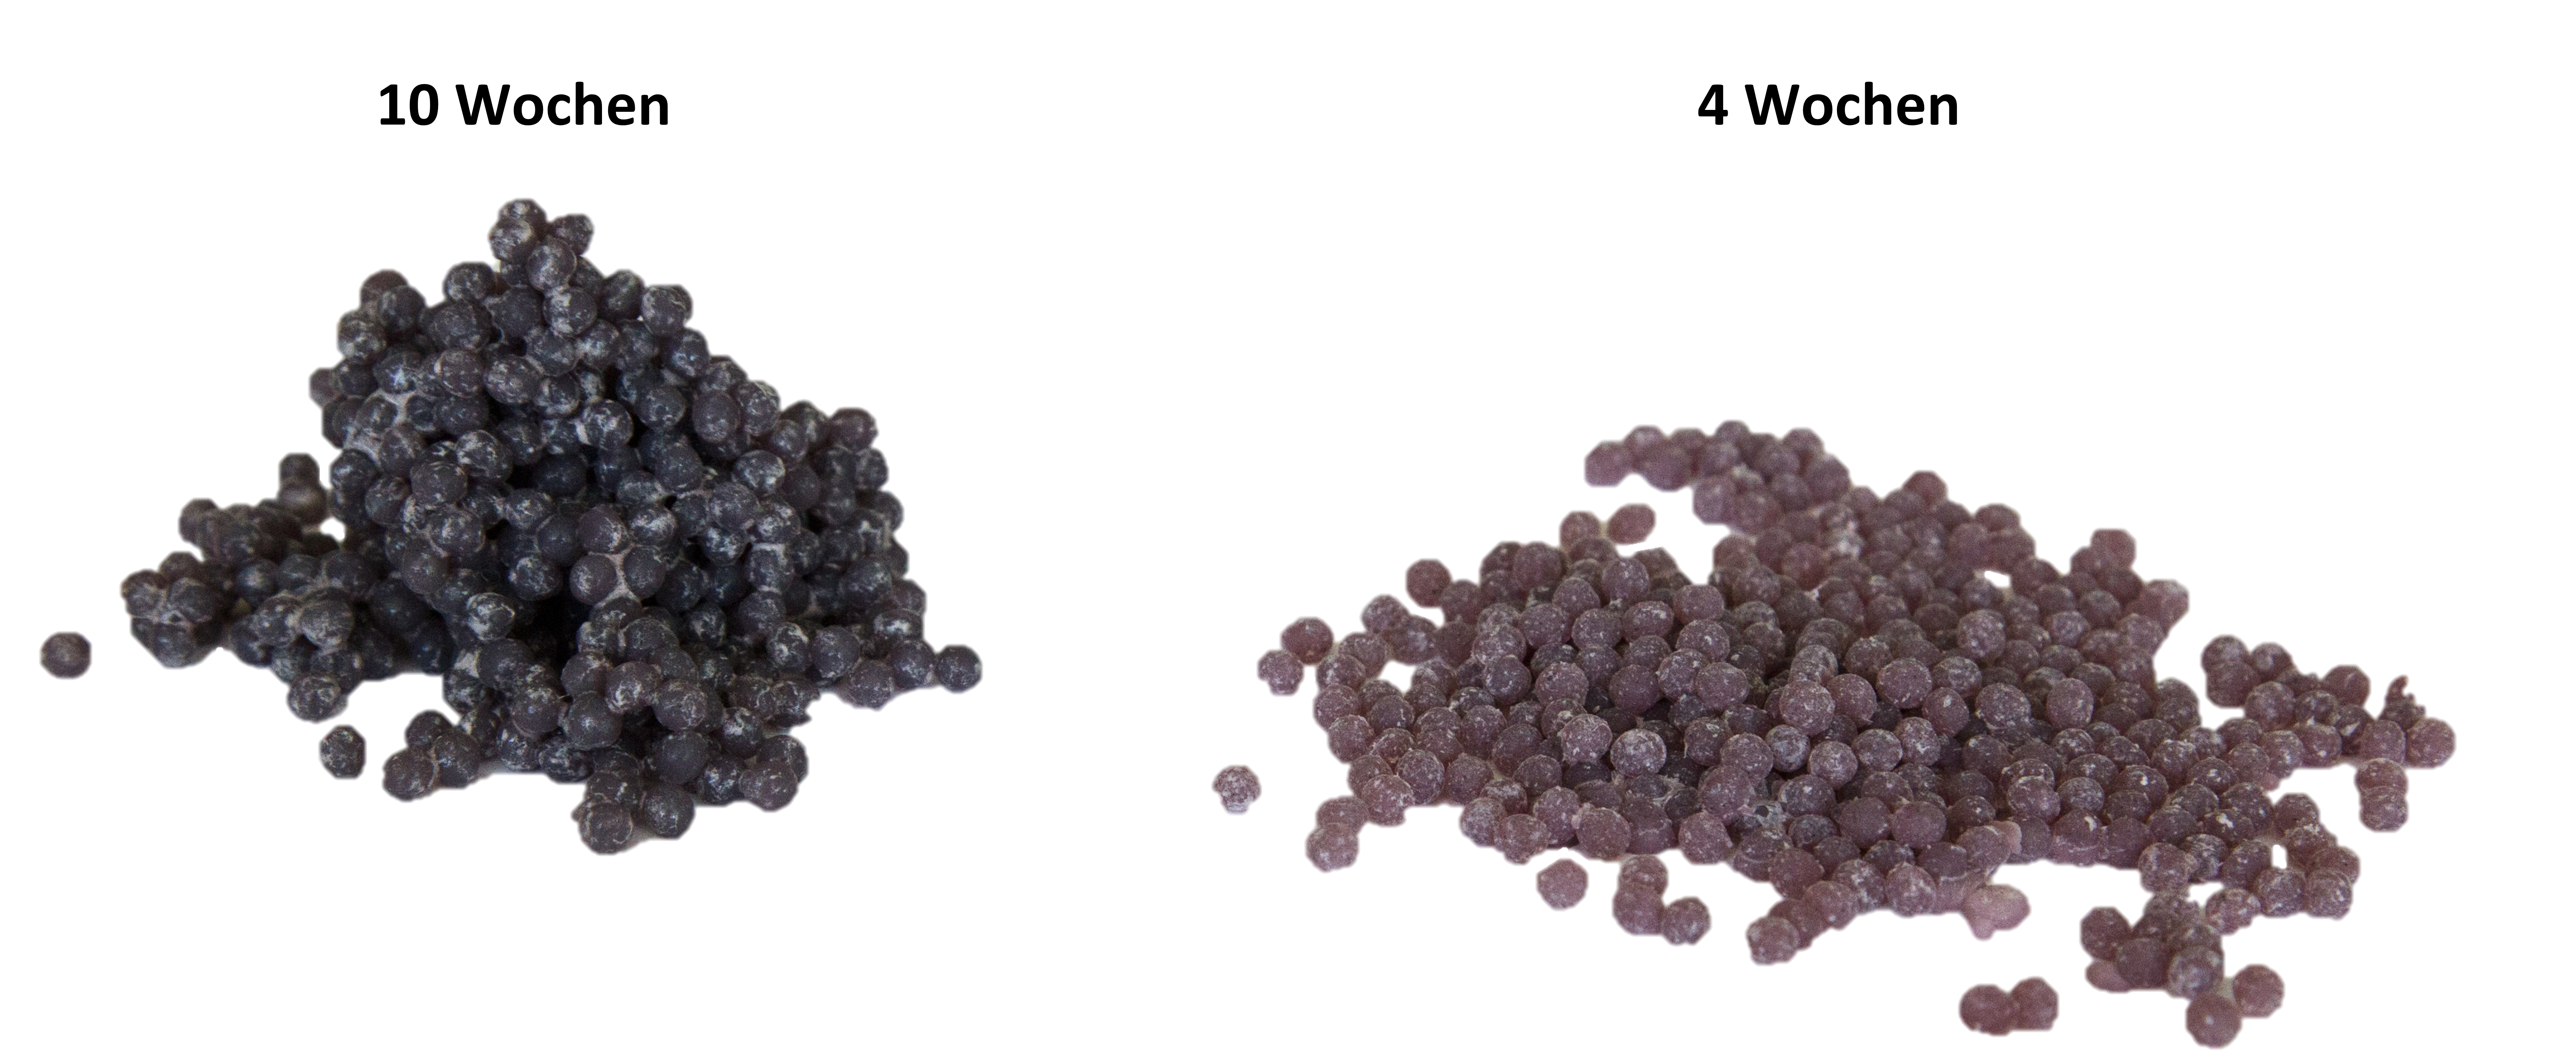
\includegraphics[draft=false,width=1\textwidth]{Illustrationen/4-Entwurf/nemacaps_altvsneu_1.jpg}
	\caption{NemaCaps bei korrekter Lagerung mit einem Alter von 10 bzw. 4 Wochen}
	\label{fig:nemacaps_altvsneu}
\end{figure}

In Abb. \ref{fig:nemacaps_altvsneu} ist der Unterschied zwischen NemaCaps welche 10 Wochen bzw. 4 Wochen alt sind, an der Farbe deutlich zu erkennen. Diese NemaCaps wurden unter korrekten Bedingungen gelagert. Dies veranschaulicht deutlich, dass nur frische NemaCaps zu Testzwecken verwendet werden sollten. Die Konsistenz der 10 Wochen alten NemaCaps ist deutlich klebriger. Diese lassen sich zu Klumpen formen und sind nur schwer vereinzelbar.

\subsubsection{Töpfe und Topferde}
Sie liegen im Fokus des Planting Robots, kleine zylindrische Container der Firma Pöppelmann, auch Blumentöpfe genannt. Um einen genauen Anhaltspunkt für die Realisierung des Setzprozesses sowie der Topferkennung zu haben, wurden die zu bestückenden Töpfe definiert. So werden zu Testzwecken ausschliesslich Töpfe des Typs VCD9, VCD11, VCD12, VCD13 und VCD14 verwendet. Abb. \ref{fig:toepfe} zeigt einen Topf des Types VCD15.

\begin{figure}[H]
	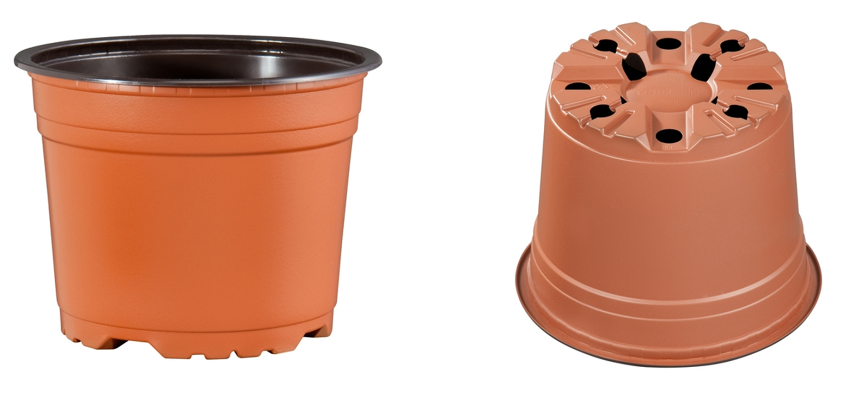
\includegraphics[draft=false,width=0.7\textwidth]{Illustrationen/4-Entwurf/VCD_Serie.png}
	\caption{Pöppelmann VCD Serie \protect\cite{Poeppelmann}}
	\label{fig:toepfe}
\end{figure}

Von substanzieller Bedeutung ist auch die verwendete Pflanzenerde. Da Erde von minderer Qualität eine hohe Menge an Fremdkörper wie Gehölz und Lehm enthalten kann. Die im Zusammenhang mit diesem Projekt verwendete Topferde ist deshalb auf die Artikel Nr.: 181 000 00 vom Hersteller RICOTER spezifiziert.

\subsection{Anforderungen}
Die in diesem Unterkapitel ausgehandelten Anforderungen an den Planting Robot dienen zur Abgrenzung des Funktionsumfangs des Projekts. Weiter sollen sie dem Industriepartner eine genaue Vorstellung darüber bieten, was er von dem fertigen Funktionsmuster erwarten kann.\\
\newline
Der Planting Robot soll stationär, auf dem Boden, neben der Topfmaschine platziert werden. Um einen präzisen Eingriff in die Produktionskette der Topfmaschine gewährleisten zu können, soll er an der Topfmaschine fixiert werden können. Der Planting Robot muss direkt am Topfkranz positioniert werden. Weiter soll der Planting Robot mit 230V Netzspannung ohne weitere Anschlüsse (z.B. Pressluft) betrieben werden können. Da der Planting Robot ein Funktionsmuster darstellt soll er nur für räumlichen Umgebungsbedingungen ausgelegt werden. \\
\newline
Der Setzprozess soll nur ausgeführt werden, wenn sich ein Topf in Position befindet. Drei Nemacaps sollen in einem Kreis mit einem Radius von 60$\%$ der Topfgrösse, mit einem Winkelabstand von jeweils 120°, in den Topf eingesetzt werden (siehe Abb. \ref{fig:Setzprozess}). Dabei soll die Einsetztiefe variabel verstellbar sein, aber maximal 60$\%$ der Topfhöhe betragen. 

\begin{figure}[H]
	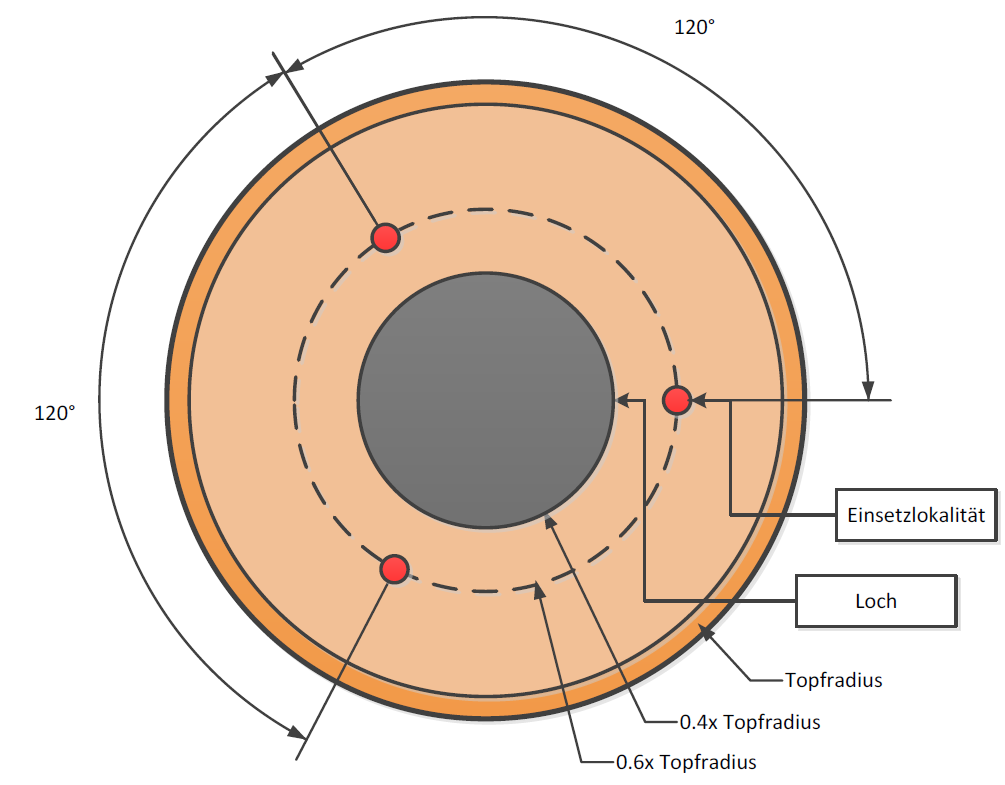
\includegraphics[draft=false,width=0.8\textwidth]{Illustrationen/4-Entwurf/Setzprozess.png}
	\caption{Setzlokalität}
	\label{fig:Setzprozess}
\end{figure}

Während eines Produktionsbatches soll sich die Topfgrösse nicht ändern. Beim Wechsel auf einen neuen Batch mit anderer Topfgrösse soll der Planting Robot umkonfiguriert werden. Eine Wunschanforderung ist es, dass sich der Planting Robot automatisch auf einen Wechsel der Topfgrösse konfiguriert. Die Setzkadenz des Planting Robots soll mit der normalen Betriebsgeschwindigkeit der Topfmaschine TC2 mithalten können. Demnach sollen 2800 Töpfe pro Stunde mit Nemacaps bestückt werden können. Wunschanforderung ist eine Produktionskapazität von 3600 Töpfen pro Stunde. Dabei ist zu beachten, dass die Eingriffszeit des Planting Robots aufgrund der Stopp- and Go-Bewegung des Topfkranzes nur 50$\%$ beträgt.
\subsection{Funktionsanalyse}

In diesem Kapitel wird der Planting Robot in verschieden Funktionsblöcke zerlegt. Die dadurch definierten Teilfunktionen ermöglichen ein systematisches Maschinendesign. Zu den jeweiligen Funktionsblöcken werden in Kapitel \ref{kap:Teilkonzept} verschiedene Lösungsvarianten ausgearbeitet. Diese Teilkonzepte werden anschliessend in Kapitel \ref{kap:LoesungsKonzept} zu einem kompletten Maschinendesign zusammengeführt.\newline
Bei der Funktionsanalyse wird zwischen einer Pflicht und einer komplexeren Wunschanforderung unterschieden. Die Wunschanforderung beschreibt zusätzlich zum vollen Funktionsumfang, eine selbstständig Konfiguration des Planting Robots auf verschieden Topfgrössen.


\begin{figure}[H]
	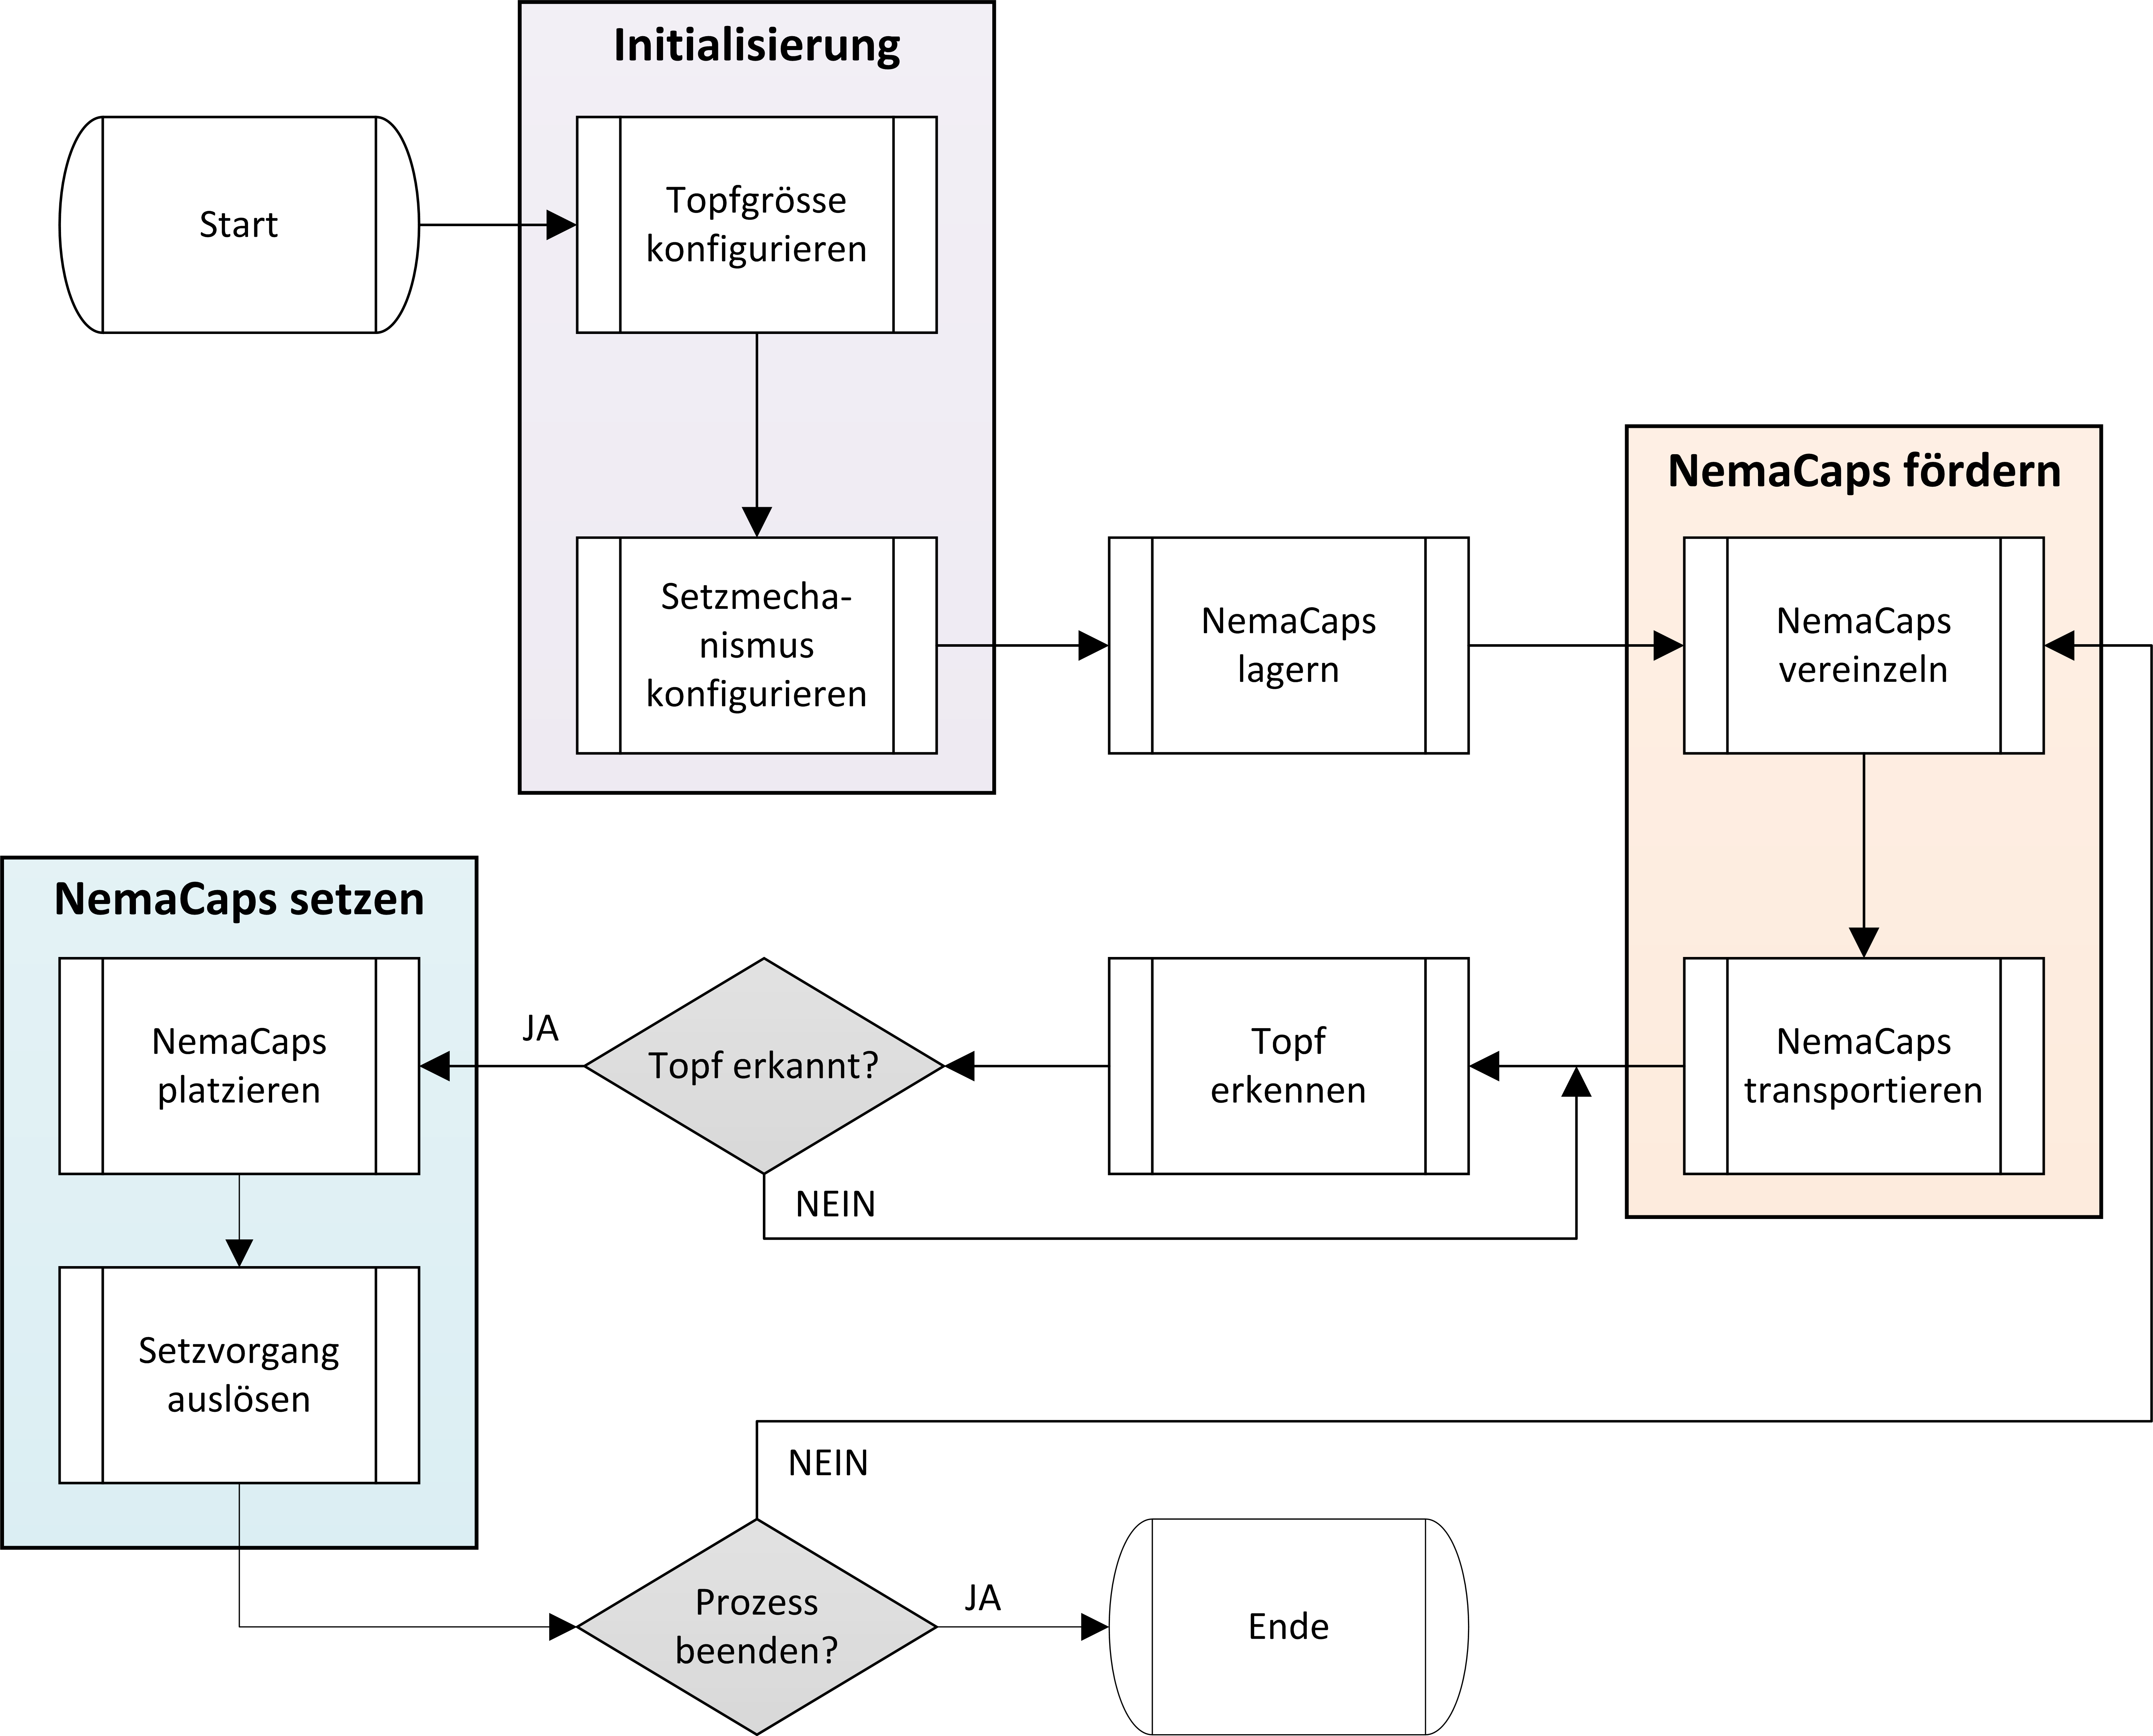
\includegraphics[width=1\textwidth]{Illustrationen/4-Entwurf/Funktionsanalyse_Pflicht.png}
	\caption{Funktionsanalyse Pflicht Blockdiagramm}
	\label{fig:FunktPflicht}
\end{figure}

\begin{itemize}
	\item \textbf{Initialisierung:} Die Initialisierung wird von einem Operator ausgeführt. Dieser Block ist nur in der Pflichtanforderung vorhanden, da die Maschine im Umfang der Pflichtanforderung die Initialisierung nicht selbstständig durchführt.
	
	\begin{itemize}
		\item \textbf{Topfgrösse konfigurieren:} In diesem Funktionsblock wird an der Maschine über ein HMI die verwendete Topfgrösse eingestellt.

		\item \textbf{Setzmechanismus konfigurieren:} Der Setzmechanismus muss für verschiedene Topfgrössen eingestellt oder ausgetauscht werden.
	\end{itemize}
	
	\item \textbf{NemaCaps lagern:} Das Setzgut (NemaCaps) wird in der Maschine mit einem Bestand von bis zu 10'000 Einheiten gelagert.
	
	\begin{figure}[H]
		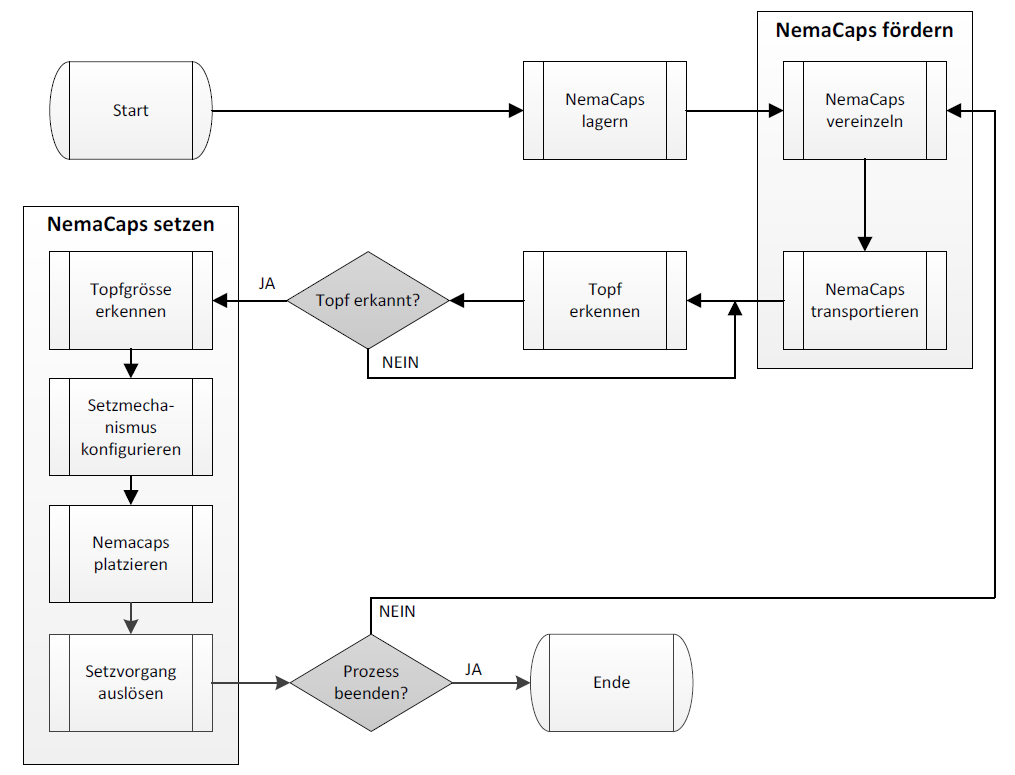
\includegraphics[width=1\textwidth]{Illustrationen/4-Entwurf/Funktionsanalyse_Wunsch.png}
		\caption{Funktionsanalyse Wunsch Blockdiagramm}
		\label{fig:FunktWunsch}
	\end{figure}
	
	\item \textbf{NemaCaps fördern:} Dieser Block behandelt die Verbindung zwischen Lager und Setzmechanismus.
	
	\begin{itemize}
		\item \textbf{NemaCaps vereinzeln:} Um die NemaCaps gezielt und kontrolliert in die Topferde einsetzen zu können, sollen diese vor dem Setzen vereinzelt werden.
		
		\item \textbf{NemaCaps transportieren:} Der Transport zwischen Lager und Setzmechanismus kann vor oder nach der Vereinzelung stattfinden.
	\end{itemize}




	\item \textbf{Topf erkennen:} Dieser Block übernimmt implizit zwei Aufgaben. Es soll erkannt werden ob überhaupt ein Topf für den Setzprozess bereit steht und ob sich dieser bewegt oder still steht. 
	
	\item \textbf{NemaCaps setzen:} Erst wenn ein Topf bereit steht wird der Setzprozess eingeleitet. Dieser unterscheidet sich wie in Abb. \ref{fig:FunktPflicht} und Abb. \ref{fig:FunktWunsch} ersichtlich zwischen Pflicht und Wunschanforderung anhand des Funktionsumfangs.
	
	\begin{itemize}
		\item \textbf{Topfgrösse erkennen:} Durch Sensorik soll die Topfgrösse jedes Topfes vermessen werden.
		
		\item \textbf{Setzmechanismus konfigurieren:} Anhand der gewonnen Daten zur Topfgrösse, soll die Maschine den Setzmechanismus selbstständig adaptieren.
		
		\item \textbf{Nemacaps platzieren:} Es folgt der eigentliche Setzprozess, in welchem die Nemacaps in einer definierten Anordnung in Position gebracht werden.
		
		\item \textbf{Setzvorgang auslösen:} Die Nemacaps welche vorher in Position gebracht wurden, werden nun in diesem Schritt vom Setzmechanismus in die Erde befördert.
	\end{itemize}
	
\end{itemize}

\subsection{Funktionsbezogene Variation}

\newpage
\section{Konzept}
\textit{(ygu)} Dieses Kapitel befasst sich mit der Ausarbeitung von drei möglichen Lösungskonzepten und deren Bewertung. Für die Auswahl der drei Lösungskonzepte wird die Methode des morphologischen Kastens von Zwicky (S.73) angewandt \cite{naefe}. In einer Tabelle werden alle gefunden Teillösungen nach Teilfunktion aufgelistet. Eine Gesamtlösung (Lösungskonzept) ergibt sich aus der Kombination von je einem Element pro Teilfunktion (Teillösung). Dabei ist bei der selektiven Wahl der Elemente auf die Verträglichkeit untereinander zu achten \cite{naefe}.
\newline
Die schiere Anzahl von möglichen Kombinationen ist ein Vorteil, kann jedoch auch überborden. Eine zu hohe Anzahl Kombinationen kann rasch zu einem Arbeitsaufwand führen, der nicht im gesetzten Zeitrahmen dieser Bachelorarbeit zu bewältigen wäre. Dieser Versuchung wird entgegnet indem sich die Auswahl auf drei Konzepte beschränkt. Weiter wird die Auswahl durch das Pflichtenheft eingeschränkt. Für diesen wiederholenden Prozess wird dabei mit Schritten "Ausscheiden und Bevorzugen" vorgegangen \cite{naefe}. Dabei werden ungeeignete Kombinationen ausgeschlossen, Kombinationen die den Fest- und Wunschanforderungen entsprechen werden bevorzugt.

Aus diesem Prozess sind drei Lösungskonzepte entstanden. Diese werden kurz vorgestellt und einer Beurteilung unterzogen. Orientiert an der Beurteilung, steht am Ende der Konzeptphase der Entscheid, welches der drei Konzepte als Funktionsmuster umgesetzt wird.

\subsection{Konzept Grau}
\textit{(ygu)} Konzept Grau besteht aus drei Teilen:
\begin{itemize}
	\item \textbf{A - Vereinzelung mittels Schöpfrohrbunker:}
	Ein Schöpfrohrbunker dient zur Vereinzelung von Kugeln. Dabei werden NemaCaps in einem trichterförmigen Behälter (Punkt 2 in Abbildung \ref{fig:konzept_grau}) gesammelt. Zu unterst im Trichter befindet sich ein Rohr (1), welches eine Translation ausübt. Durch die Translation wird das unterste Gefüge so bewegt, dass ein oder mehrere NemaCaps ins Rohr fallen. So werden die NemaCaps in einer Reihe geordnet.
	
	\item \textbf{B - Auslösen und Transport mittels Pneumatik:}
	Aufeinander gestapelt, werden die NemaCaps von der Auslösung abgefertigt. Dabei wird das unterste NemaCaps mit einer linearen Bewegung (3) zu einer Öffnung geschoben. Zusätzlich wird das NemaCap an der Öffnung durch ein Vakum angesaugt. Durch einen Schlauch wird das NemaCap mittels Pneumatik zur Einsetzlokalität transportiert. 
	
	\item \textbf{C - Setzen mittels Rohr:}
	Zeitgleich zu Phase A und B wird am Topf das Setzen der NemaCaps vorbereitet. Dafür wird ein Rohr (4) in den stehenden Topf bis zur Setztiefe eingetaucht. Ist dieser eingetaucht, wird das NemaCap durch die Pneumatik zum Rohrende transportiert und somit im Topf platziert. Das Rohr fährt aus dem Topf, der Prozess beginnt von vorne.
\end{itemize}

Die Konfiguration des Setzmechanismus wird dabei durch die radiale Verstellung der einstechenden Rohre gewährleistet. Hierfür ist die manuelle Einstellung des Rohrs in radialer Richtung notwendig und vor jedem Batch auszuführen.

Dabei muss gewährleistet sein, dass das eintauchende Rohr nicht durch Erdpartikel verstopft wird.
\begin{figure}[H]
	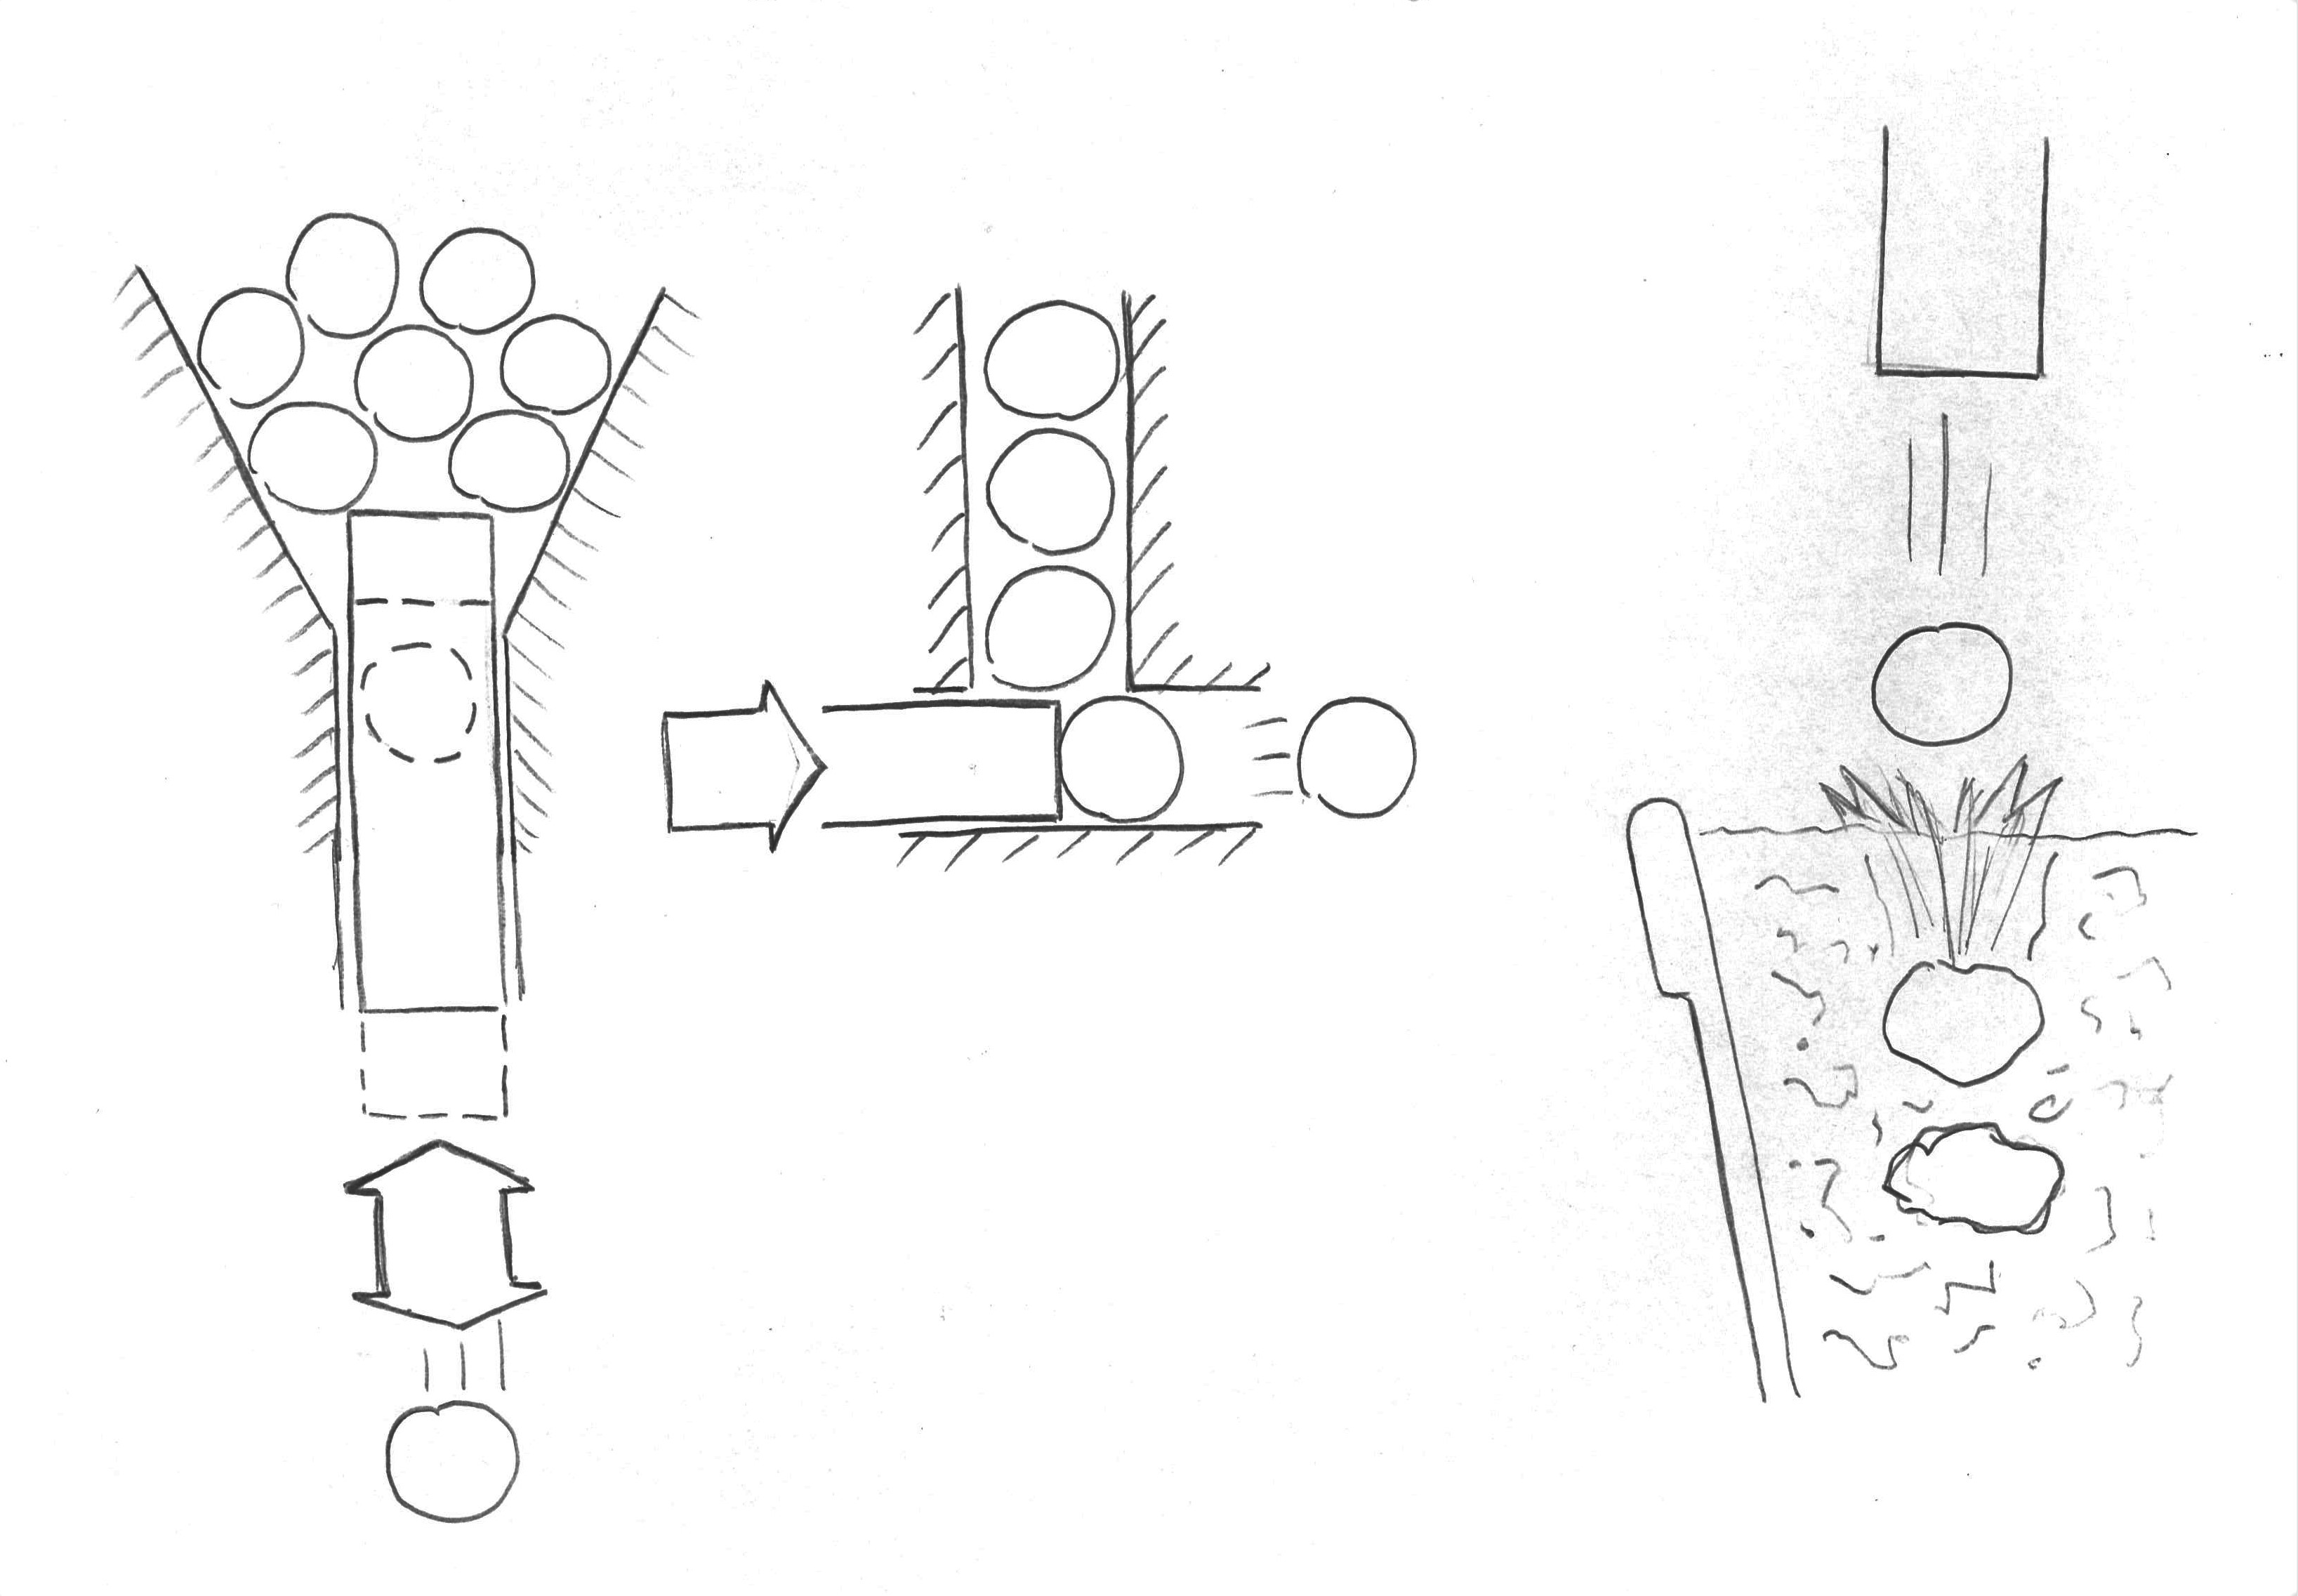
\includegraphics[scale=0.6]{Illustrationen/5-Konzept/grau_Konzept.jpg}
	\caption{Konzeptskizze von Konzept Grau}
	\label{fig:konzept_grau}
\end{figure}

\input{Kapitel/5_Konzept/5.2_Konzept_Grün}
\subsection{Konzept Blau}

\textbf{Rotierende Lochmaske}
\newline
\begin{wrapfigure}[26]{r}{10cm}
	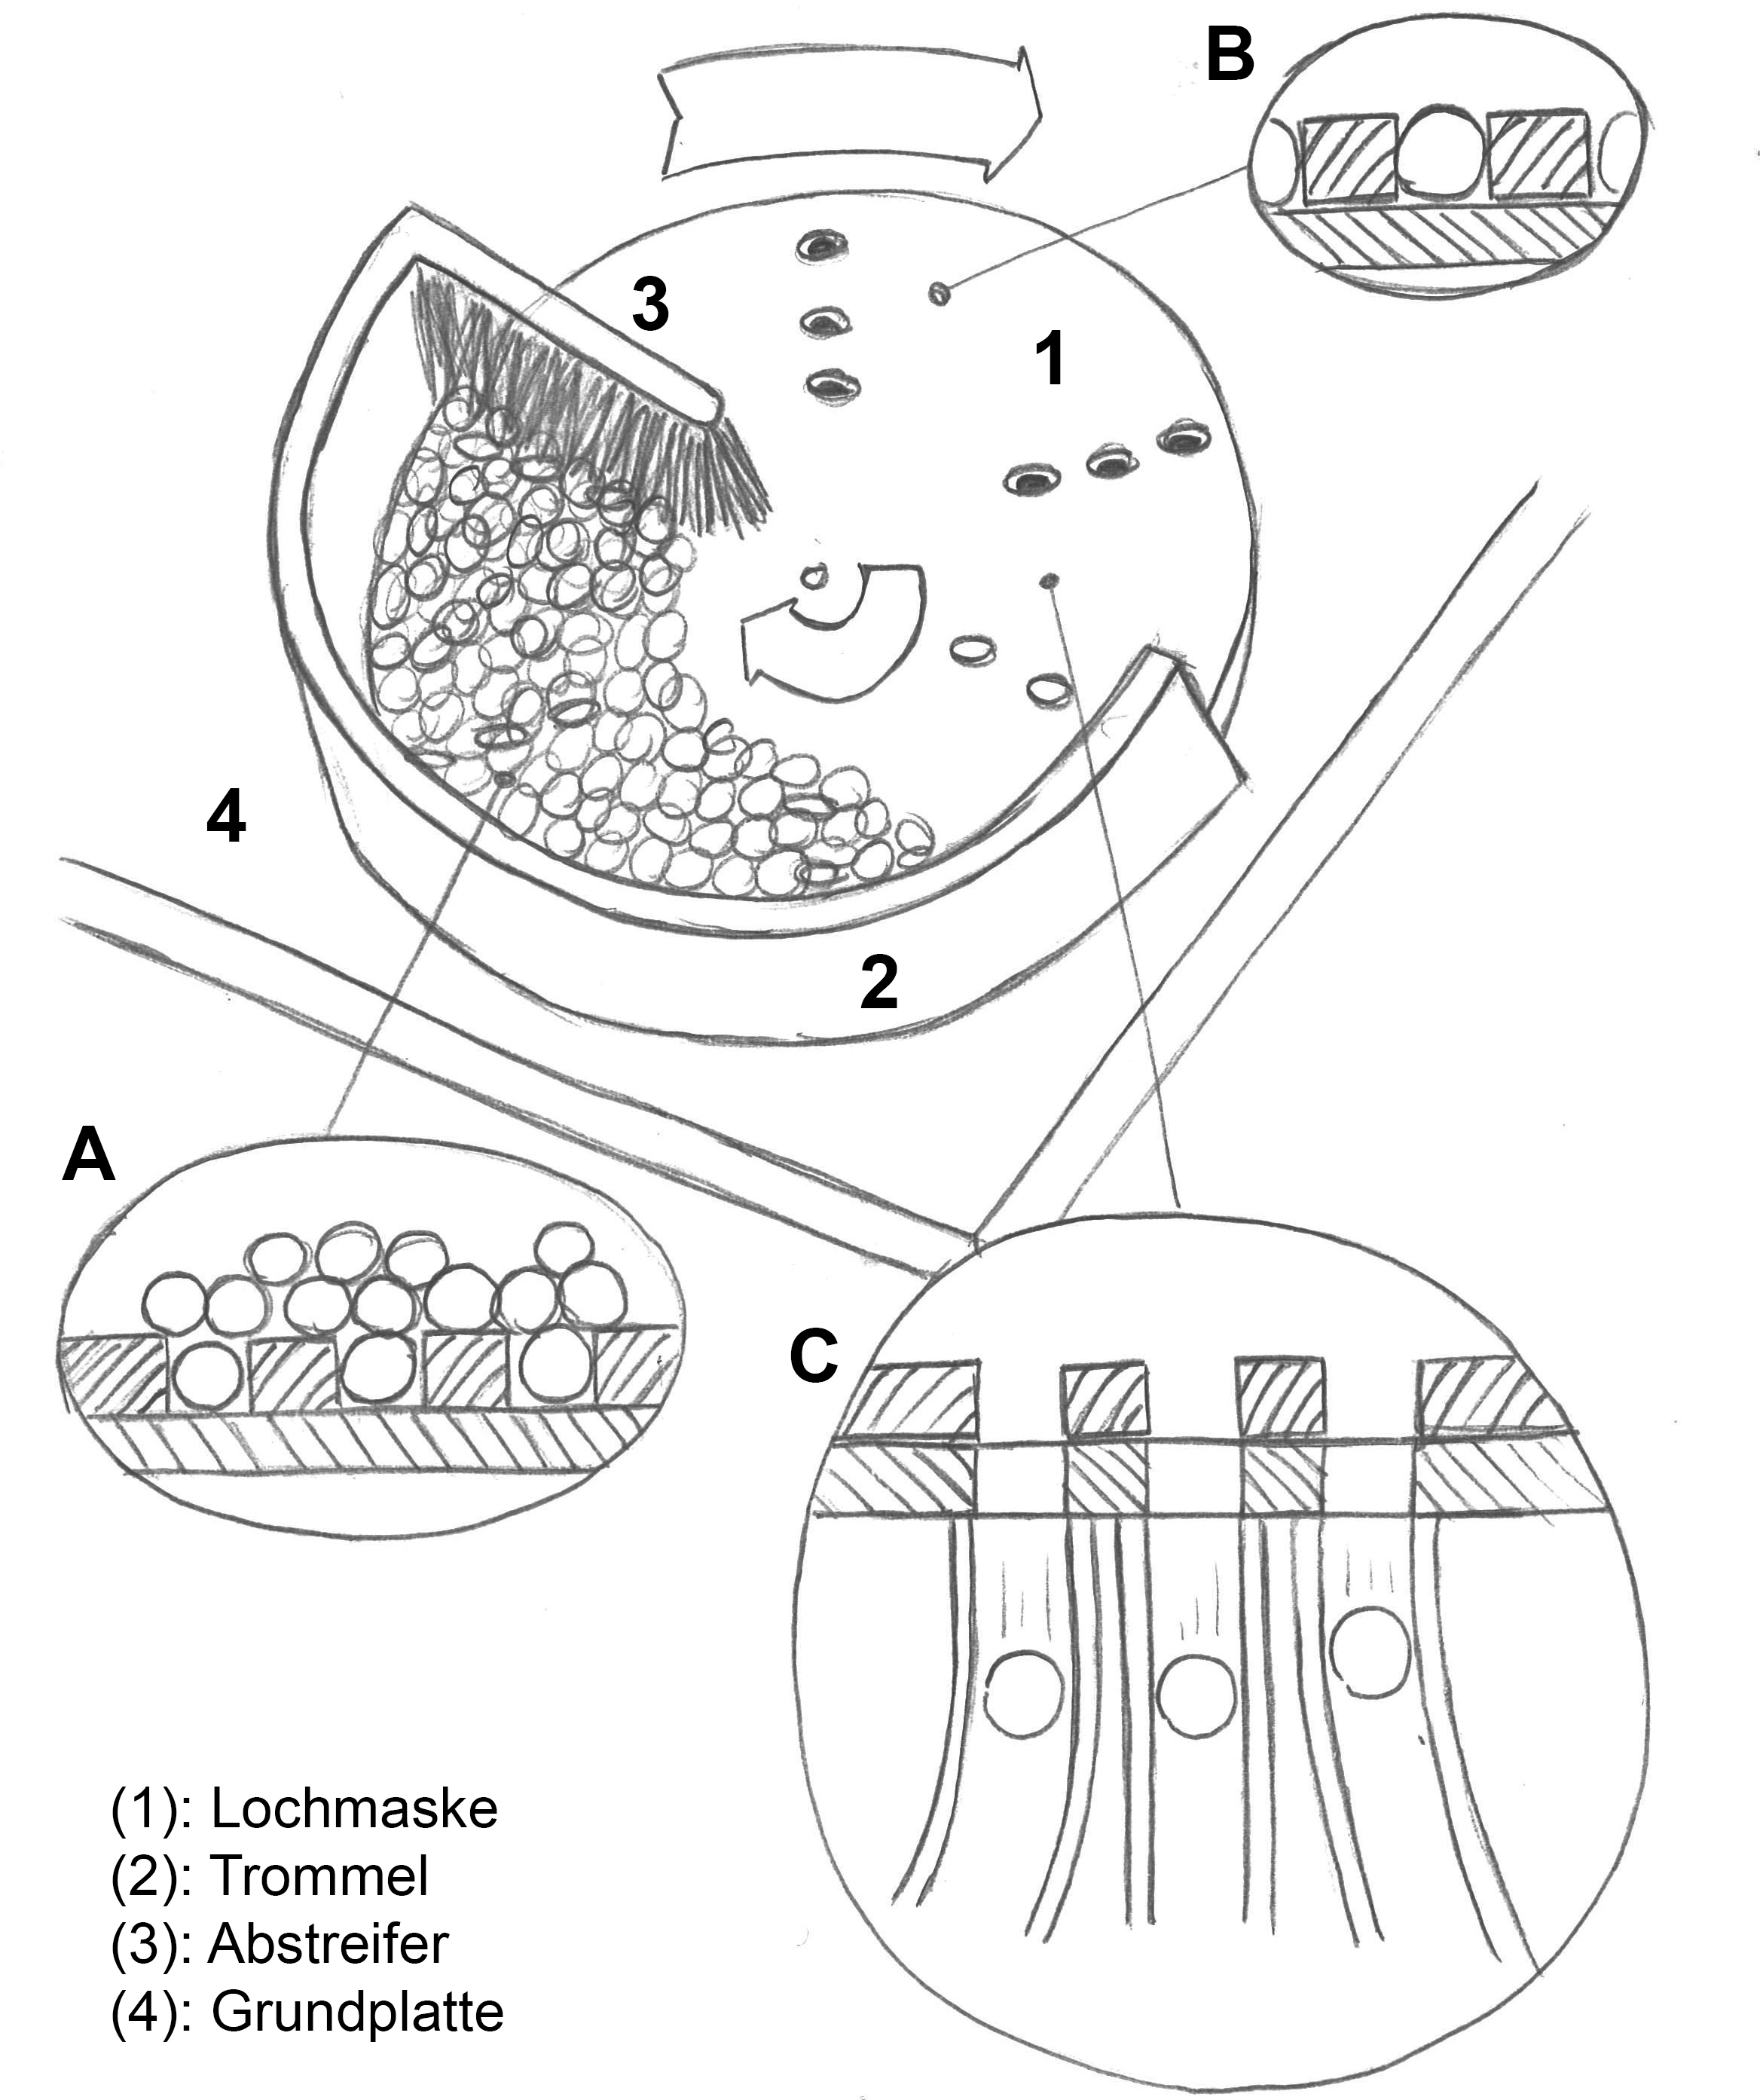
\includegraphics[scale=0.52]{Illustrationen/5-Konzept/schema_vereinzelung.jpg}
	\caption{Vereinzelung durch rotierende Lochmaske}
	\label{fig:schema_vereinzelung}
\end{wrapfigure}
Ein weiteres Konzept ist die Vereinzelung durch eine rotierende Lochmaske. Dabei werden die NemaCaps in einen Behälter gefüllt (Punkt 2 in Abbildung \ref{fig:schema_vereinzelung}). Im Behälter befindet sich eine rotierend gelagerte Scheibe mit Löchern (Lochmaske, 1). Die Löcher sind so gross, dass gerade ein NemaCap darin Platz hat. Durch die Rotation der Lochmaske fallen nun NemaCaps in die Maske (Detail A) und werden zu Detail B transportiert. Ein Abstreifer (hier in Form einer Bürste) sorgt dafür, dass überschüssige NemaCaps zurückgehalten werden. In der Grundplatte (4) sind Löcher vorgesehen, sodass bei Detail C die NemaCaps in Schläuche fallen. Idealerweise wird dieser Aufbau schief gelagert. 
\newline
\subsection{Funktionsnachweis kritischer Funktionen}
\label{funktionsnachweis}
\textit{(ygu)} Dieses Unterkapitel befasst sich mit dem praktischen Nachweis von kritischen Teilfunktionen. Kritische Teilfunktionen sind Funktionen, welche bei einem Ausfall, einen Ausfall des Gesamtsystems zur Folge hat. Daher wird die technische Machbarkeit dieser Teillösungen zusätzlich überprüft. Einfach aufgebaute aber funktionell ähnliche Versuche werden realisert. An diesen Aufbauten wird dann der praktische Nachweis erbracht, ob die techische Umsetzbarkeit realistisch erscheint. Diese Beurteilung wird für Bewertung der ausgearbeiteten Lösungskonzepte miteinbegezogen.
\newline
Bei Betrachtung der Funktionsanalysen (Abbildungen \ref{fig:FunktPflicht} und \ref{fig:FunktWunsch}) ist erkennbar, dass beide Varianten (Pflicht sowie Wunsch) eine Serieschaltung darstellen.  Bei der Umsetzung einer Maschine mit einfacher Redundanz ergibt dies implizit, dass jede Funktion als kritisch eingestuft wird. Aus zeitlichen Gründen kann ein umfassenden Nachweis von allen Teillösungskonzepten nicht abschliessend durchgeführt werden. Für den Nachweis ist eine pragmatische Auswahl notwendig. Es werden daher nur Funktionen mit erhöhtem Ausfallrisiko und einer vielversprechenden Funktionserfüllung überprüft.

\subsubsection{NemaCaps vereinzeln und fördern}
Die Automatisationsbranche setzt sich vertieft mit der Förderung und Vereinzelung von Gütern auseinander. Die automatisierte Sortierung sowie Transport eines Gutes sind grundlegende Bedingungen, sodass ein Produkt überhaupt in der automatisierten Serienfertigung herstellbar wird. Da solche Lösungen vielfach beide Funktionen miteinander vereinen, werden diese gemeinsam in einem Unterkapitel untersucht.
\newline
\newline
\textbf{Vibrationswendelförderer}
\newline
Der Vibrationswendelförderer ist ein Bestandteil von Konzept Grün. Die detaillierte Funktionsweise des Vibrationswendelförderers wurde bereits im Kapitel \ref{KonzeptGreen} erläutert.
\newline
Aus vergangenen Studentenarbeiten besitzt die HSLU T\&A solch ein Wendelförderer. Dimensioniert ist dieser für die Vereinzelung von gezuckerten Mandeln. Auch wenn dadurch die Vereinzelung nur bedingt funktionsfähig ist, eignet sich dieses Gerät zur ersten Überprüfung mit NemaCaps. 

Praktische Tests mit NemaCaps konnten am 15.3.2017 am Wendelförderer durchgeführt werden. NemaCaps wurden ins Haufwerk (Punkt 1 in Abbildung \ref{fig:wendelfoerderer}) eingefüllt und der Wendelförderer gestartet. Durch die Vibration sammelten sich die NemaCaps im Wendel (2) und begannen zu wandern. Die Förderung klappte einwandfrei, wobei die rasche Transportgeschwindigkeit positiv überraschte. 
\begin{figure}[H]
	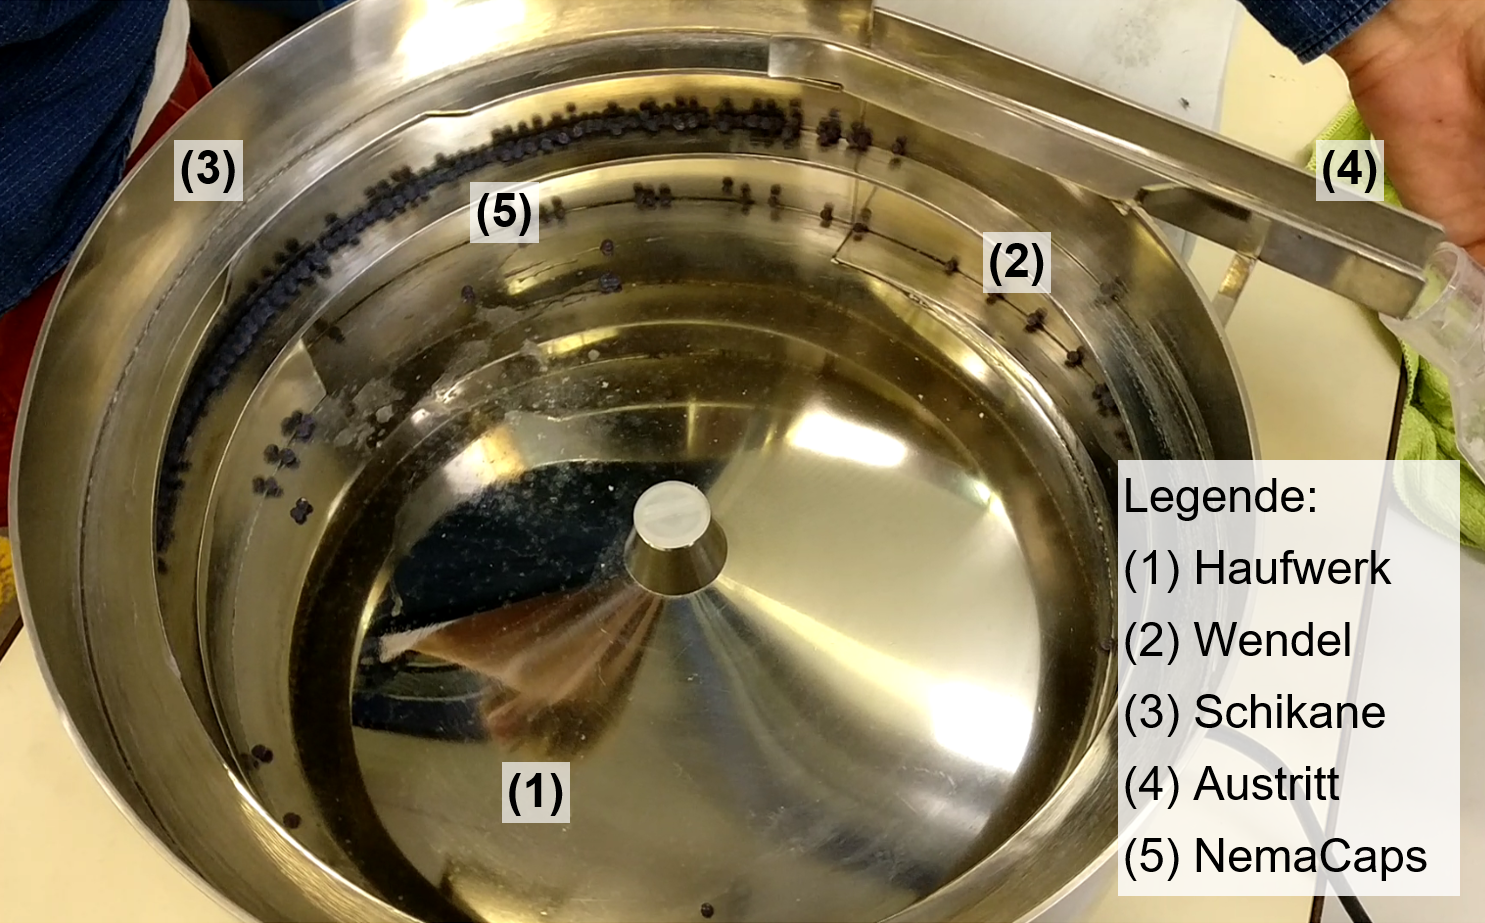
\includegraphics[width=1\textwidth]{Illustrationen/5-Konzept/wendelfoerderer.PNG}
	\caption{Praktische Tests am Wendelförderer der Hochschule}
	\label{fig:wendelfoerderer}
\end{figure}
\textbf{Erkenntnisse}
\newline
Folgende Erkenntnisse lieferten die Versuche:
\begin{itemize}
	\item Eine Förderung von NemaCaps mit einem Wendelförderer ist möglich. Die NemaCaps eignen sich als Fördergut und werden mit einer hohen Zuverlässigkeit gefördert.
	
	\item Die Schikane erfüllt ihre Funktion nicht. Dies ist allein auf die Tatsache zurückzuführen, dass der verwendete  Wendelförderer für gezuckerte Mandeln dimensioniert wurde. Eine Anpassung der Schikanen auf NemaCaps ist technisch machbar.
	
	\item Die Umsetzung der Funktionen 'NemaCaps vereinzeln' und 'NemaCaps fördern' mit einem Wendelförderer ist aus rein technischer Sicht realisierbar.
\end{itemize} 
\newpage
\textbf{Vereinzelung durch Lochmaske}
\newline
Die Vereinzelung durch eine rotierende Lochmaske ist Teil von Konzept Blau. Der praktische Funktionsnachweis wird anhand eines einfachen Funktionsmusters erbracht. Eine manuell drehbare Lochmaske wird dabei auf einer schief gelagerten Grundplatte montiert (siehe Abbildung \ref{fig:funktmuster_vereinzelung}). Auf der Grundplatte ist eine gewölbte Wand verklebt, die zur Lagerung der NemaCaps dient. Das Design des Funktionsnachweises ist jenem der Firma Kofatec GmbH angelehnt. Die Lochmaske wird für einen ersten Funktionsnachweis von Hand betrieben.
\begin{figure}[H]
	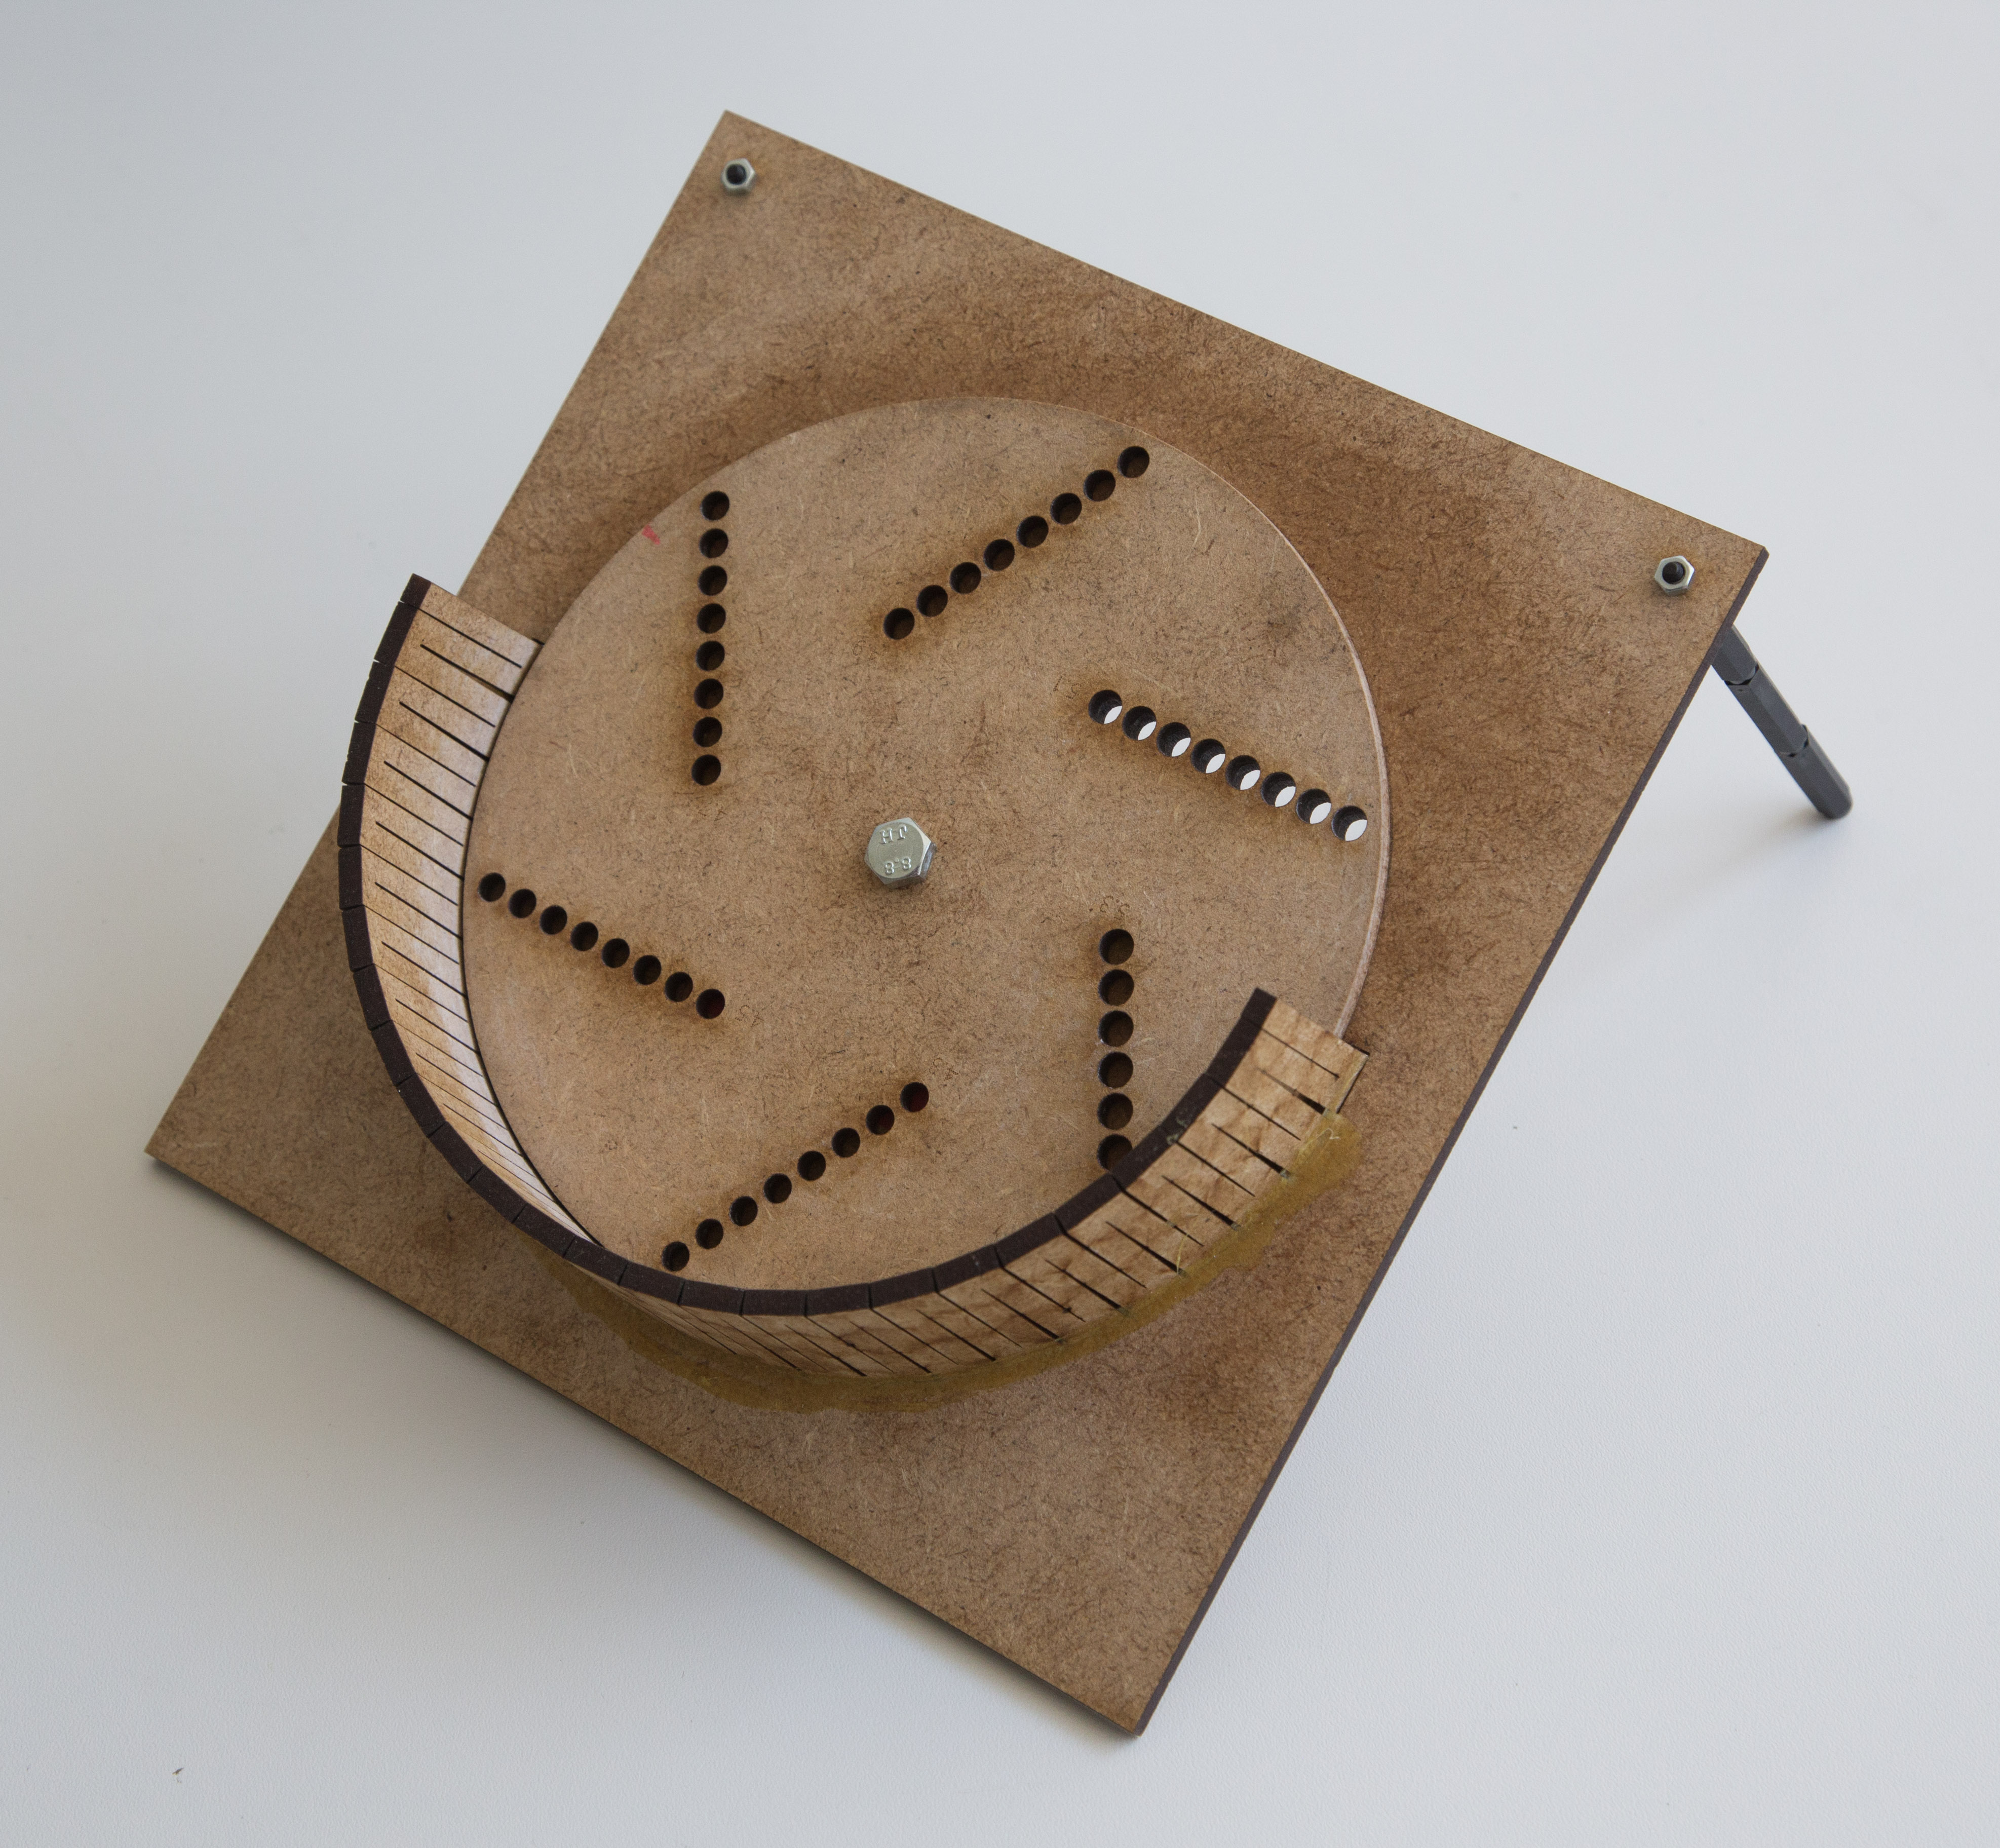
\includegraphics[width=1\textwidth]{Illustrationen/5-Konzept/funktmuster_vereinzelung.jpg}
	\caption{Teilfunktionsmuster zur Vereinzelung der NemaCaps}
	\label{fig:funktmuster_vereinzelung}
\end{figure}
Am 21.3.2017 wurde am umgesetzten Funktionsmuster der Funktionsnachweis durchgeführt. Durch zielgerichtetes Ausprobieren von verschiedenen Durchmesser der Löcher wurde die Lochmaske für die NemaCaps ausgelegt. Anschliessend wurde mittels manuellem Rotieren die Vereinzelung überprüft.
\begin{figure}[H]
	\includegraphics[width=1\textwidth]{Illustrationen/5-Konzept/funktion_vereinzelung.jpg}
	\caption{Funktionsnachweis der Vereinzelung}
	\label{fig:funktion_vereinzelung}
\end{figure}
Folgende Erkenntnisse lieferten die Versuche:
\begin{itemize}
	\item Die Lochmaske nimmt zuverlässig NemaCaps auf (Siehe Punkt 2 und Detail A in Abb. \ref{fig:funktion_vereinzelung}). Auch ein Transport zur Auslösung verläuft problemlos.
	
	\item Die Abstreifung von NemaCaps funktioniert. Kritisch ist dabei jedoch die Wahl des Abstreifers. Verwendet man scharfkantige Gegenstände kann es passieren, dass NemaCaps beschädigt werden. Weiter wurde erkannt, dass NemaCaps heikel auf Scherkräfte reagieren.
		
	\item Die Zuverlässigkeit der Auslösung am Punkt 3 in Abb. \ref{fig:funktion_vereinzelung} ist durchschnittlich. Dies wird damit erklärt, dass nicht frische NemaCaps verwendet wurden. Dadurch hat sich das hygroskope Pulver in Wasser gewandelt und so die Adhäsion der NemaCaps erhöht. Dadurch blieben geschätzte 50 Prozent der NemaCaps an der Lochmaske hängen. Auch ist ein holzfaserbasiertes Material (wie MDF) für die Lochmaske ungeeignet. Die rauhe Oberfläche der Bohrung bietet so mehr Haftung.
	
	\item Durch leichtes Antippen der Grundplatte oder einem Luftstoss konnten alle NemaCaps ausgelöst werden. Dies zeigt, dass durch Abhilfemassnahmen durchaus eine höhere Zuverlässigkeit erreicht wird.
	
	\item Die Umsetzung von diesem Lösungsansatz ist nur realistisch, wenn klare Abhilfemassnahmen und Verbesserungen der Lochmaske zur Steigerung der Zuverlässigkeit definiert werden. 
\end{itemize} 


\subsubsection{NemaCaps setzen}
Der Lösungsansatz der Teilfunktion 'NemaCaps setzen' basiert auf der Idee, in einem ersten Schritt ein Loch auszuheben oder Erde zu verdrängen und anschliessend ein NemaCap in die Vertiefung fallen zu lassen. Ein ähnlicher Ansatz verfolgt die Idee, mit einer spitzen Zange Erde zu verdrängen, die Zange im Erdreich zu öffnen und dort ein NemaCap zu platzieren. Schematisch dargestellt sind beide Ansätze in Abbildung \ref{fig:skizze_setzversuch}.
\newline
Um die Umsetzbarkeit dieser Ideen zu überprüfen, werden zwei Versuche durchgeführt:
\begin{itemize}
	\item \textbf{A) Ermittlung der Verdrängkraft:} Mit einer konventionellen Setzhilfe aus dem Gartenbau werden praktische Tests durchgeführt. Ein Topf wird mit dem vorgegebenen Gartenhumus von Ricoter befüllt und leicht angepresst. Anschliessend wird die maximale Einsetztiefe an der Setzhilfe markiert und schrittweise mit Gewicht (Masse m in Abbildung \ref{fig:skizze_setzversuch}) beschwert. Sobald die Markierung den Gartenhumus berührt, wird die Setzhilfe inklusive Masse m gewogen und durch die Multiplikation mit der Erdbeschleunigung die benötigte Verdrängungskraft ermittelt.
		
	\item \textbf{B) NemaCap mittels Zange setzen:} Der identische Versuch wird mit der genannten Zange durchgeführt, wobei die geschlossene Zange ein NemaCap gegeben wird. Bei Erreichung der Setztiefe wird die Zange geöffnet und das NemaCap platziert (siehe Abbildung \ref{fig:skizze_setzversuch}).
\end{itemize} 

\begin{figure}[H]
	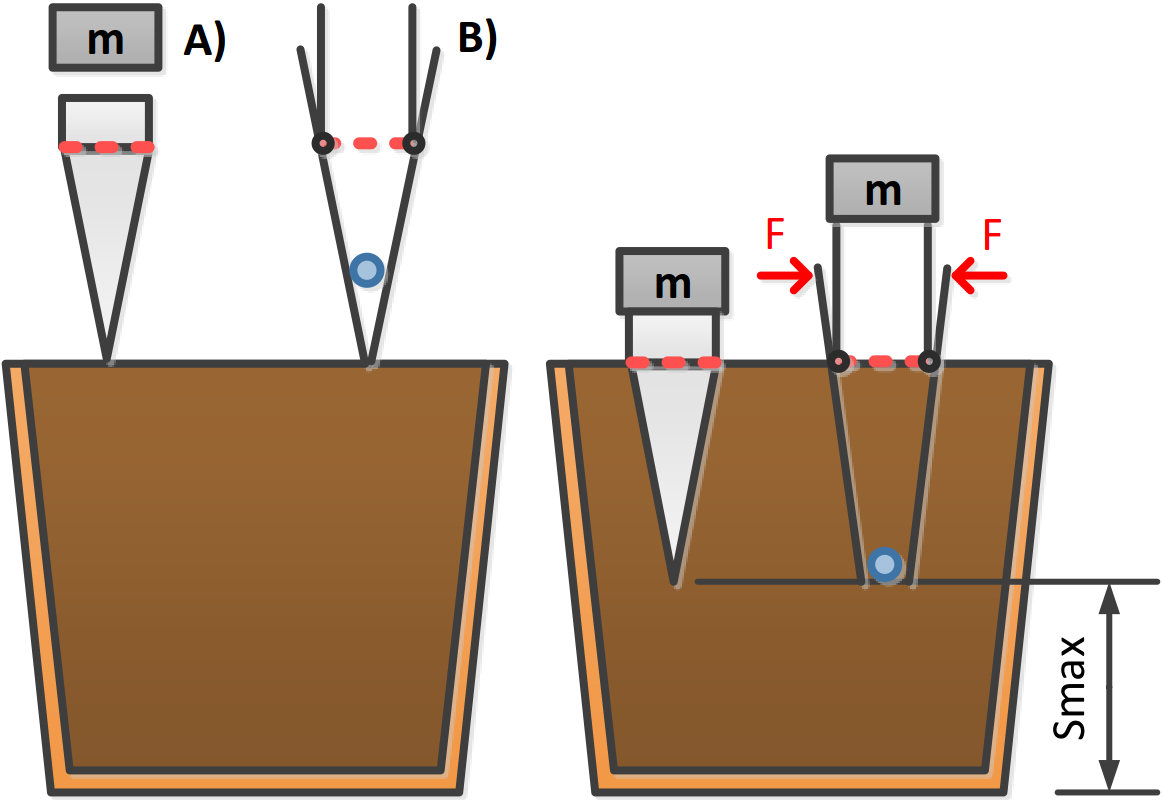
\includegraphics[width=1\textwidth]{Illustrationen/5-Konzept/skizze_stechversuch.PNG}
	\caption{Versuchsaufbau zur Ermittlung der Verdrängkraft}
	\label{fig:skizze_setzversuch}
\end{figure}

\textbf{Erkenntnisse}
\newline
Folgende Erkenntnisse lieferten die Versuche:
\begin{itemize}
	\item Mit der konventionellen Setzhilfe kann mit geringem Aufwand das erforderliche Setzloch verdrängt werden. Auch bei erschwerten Umständen wie komprimiertem Gartenhumus oder kleinerem Gehölz konnte ein Setzloch verdrängt werden. Über mehrere Versuche wurden folgende Werte ermittelt:
\begin{table}[H]
	\begin{tabular}{|l|c|c|}
		\hline 
		& kleinster Topf (D=90mm) & grösster Topf (D=140mm) \\ 
		\hline 
		geforderte Setztiefe [mm] & 40 & 64 \\ 
		\hline 
		benötigte Masse [kg] & 0.15 & 0.6 \\ 
		\hline 
		Verdrängungskraft[N] & 1.5  & 6.0  \\ 
		\hline 
	\end{tabular} 
	\caption{Ermittelte Verdrängungskraft durch Versuche}
	\label{tab:verdraengungskraft}
\end{table}	
	
	\item Der gegebene Gartenhumus von Ricoter besitzt gute Eigenschaften für diese Anwendung. Nach der Verdrängung behält das Setzloch seine Form bei, sodass die Bedingungen für das Einsetzen des NemaCaps gegeben sind. Dabei ist darauf zu achten, dass stets frischer Gratenhumus verwendet wird.
	
	\item Tests mit der Zange ergaben, dass eine Verdrängung der Erde mit dem identischen Kraftaufwand machbar ist. Um die Zange in der erforderlichen Setztiefe zu öffnen und das NemaCap zu platzieren, wird ein erhöhter Kraftaufwand benötigt. Wie eine Streckenlast wirkt die zu verdrängende Erde der Bewegung entgegen und erschwert die Öffnung. Diese Teillösung wird als nicht umsetzbar bewertet.
\end{itemize} 

\subsubsection{Setzmechanismus konfigurieren}
Die automatische Konfiguration des Setzmechanismus ist als Wunschanforderung im Pflichtenheft formuliert. Gemeint ist dabei die automatische Verstellung der Radien der Einsatzlokalität. Ein ausgearbeiteter Lösungsansatz basiert auf zwei Kulissen, welche ingsesamt drei Dorne halten. Über die Rotation der einen Kulisse kann der Dorn radial verstellt werden. Umgesetzt werden die Kulissen als kreisförmige Scheiben (Punkt 1 in Abbildung \ref{fig:setzmech_konfig}), welche über eine innere Kulisse (Punkt 2 in Abb. \ref{fig:setzmech_konfig}) synchron verstellt werden. Dabei wird dieses Funktionsmuster manuell von Hand betrieben.
\begin{figure}[H]
	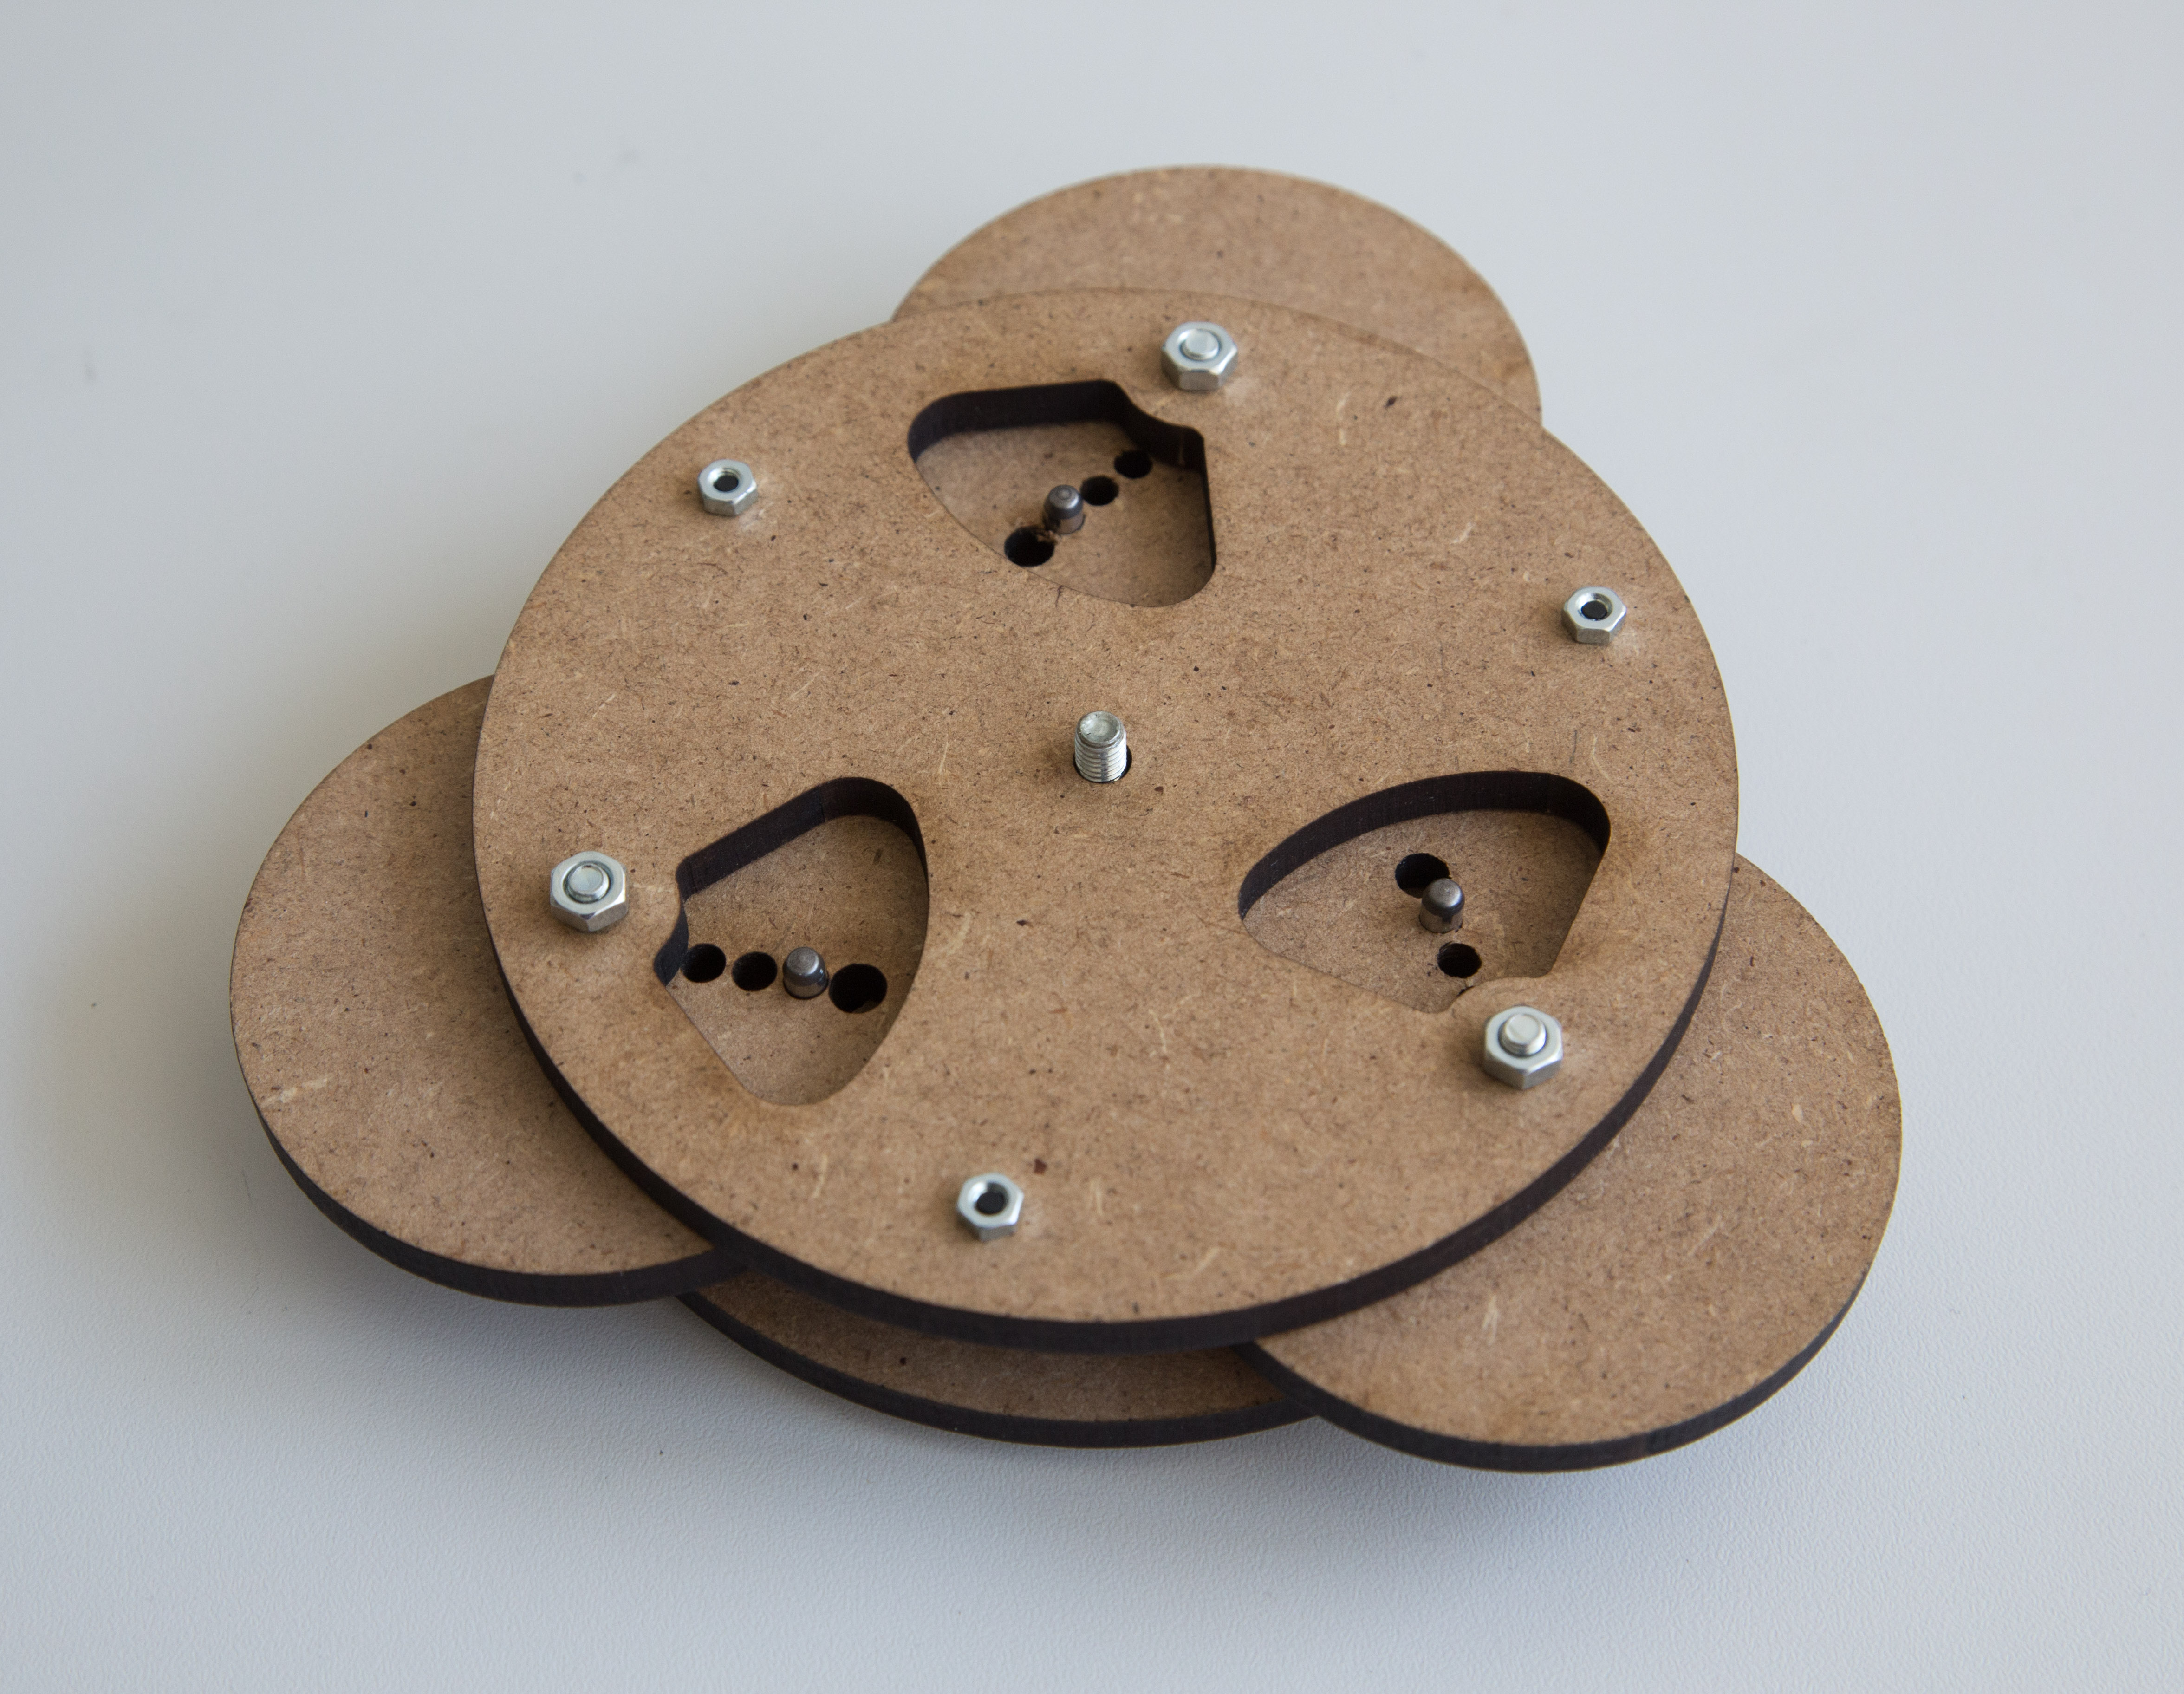
\includegraphics[width=1\textwidth]{Illustrationen/5-Konzept/setzmech_konfig.jpg}
	\caption{Teilfunktionsmuster zur Konfiguration des Setzmechanismus}
	\label{fig:setzmech_konfig}
\end{figure}
Folgende Erkenntnisse lieferte das Funktionsmuster:
\begin{itemize}
	\item Die manuelle Verstellung des Radius mittels Kulisse ist möglich. Durch eine Drehbewegung werden die Dornen synchron verstellt.
	
	\item Aus der Geometrie der Kulissen wird erkennbar, dass die maximale Rotation 45° beträgt. Dies muss bei einer allfälligen Evaluation des Antriebs berücksichtigt werden.
	
	\item Am Rand der Kulisse nimmt der Kraftaufwand für eine Verstellung deutlich zu. Es kommt auch vor, dass die Kulisse am Rand kaum in Bewegung gerät. Dies ist damit erklärbar, dass an diesem Punkt die Wirkungslinien der Kulissen normal zueinander stehen und so kein Moment auf die äussere Kulisse wirken kann. Bei einer allfälligen Umsetzung müssen die Wirkungslinien der Kulissen möglichst parallel verlaufen. 
\end{itemize} 
\subsubsection{Topferkennung}
\subsection{Bewertung und Entscheid}
\textit{(ygu)} Für die Bewertung der Konzepte wird eine Nutzwertanalyse durchgeführt \cite{naefe}. Angepasst auf die vorliegende Bachelorarbeit ergibt sich folgendes Vorgehen:

\begin{enumerate}
	\item \textbf{Erkennen der Bewertungskriterien:} Für die objektive Bewertung der Konzepte werden Bewertungskriterien definiert.
	
	\item \textbf{Gewichtung der Kriterien:} Für jedes Kriterium wird ein Gewichtungsfaktor festgelegt, um die Kriterien nach ihrer Wichtigkeit einzuordnen.
	
	\item \textbf{Beurteilen nach Wertvorstellung:} Mit der definierten Wertskala nach VDI-Richtlinie 2225 werden die einzelnen Konzepte an den definierten Kriterien bewertet \cite{vdi2225}.

\begin{table}[H]
	\begin{tabular}{|c|l|}
		\hline 
		\textbf{Punkte} & \textbf{Bedeutung} \\ 
		\hline 
		0 & unbefriedigend \\ 
		\hline 
		1 & gerade noch tragbar \\ 
		\hline 
		2 & ausreichend \\ 
		\hline 
		3 & gut \\ 
		\hline 
		4 & sehr gut (ideal) \\ 
		\hline 
	\end{tabular} 
	\caption{Wertskala nach VDI-Richtlinie 2225}
	\label{tab:wertskala}
\end{table}	
	
	
	\item \textbf{Bestimmung des Nutzwertes:} Aus der Bewertung wird der Nutzwert von jedem Konzept ermittelt. Das bestbewertete Konzept wird umgesetzt.
\end{enumerate}

\subsubsection{Definition und Gewichtung der Kriterien}
\textit{(ygu)} Bei der Definition der Kriterien ist darauf zu achten, dass jedes einzelne Kriterium relevant für die grundlegende Aufgabenstellung ist.
Als Orientierung wurde die „Leitlinie mit Hauptmerkmalen zum Bewerten in der Konzeptionsphase“ verwendet \cite{pahl}. 
\newline
Die Kriterien beinhalten folgende Punkte:
\begin{itemize}
	\item Komplexität
	\begin{itemize}
		\item Geringer Grad der technischen Komplexität
		
		\item gebräuchliche Fertigungsverfahren, keine aufwendige Vorrichtungen, einfach gestaltete Teile
		
		\item leichte und schnelle Montage
	\end{itemize}

	\item Risiken
	\begin{itemize}
	\item Funktionserfüllung mit ausreichender Wirkung und geringen Störgrössen
	
	\item Hohe Zuverlässigkeit während dem Betrieb
	
	\item abschätzbare Risiken in der Umsetzung
	\end{itemize}

	\item Kosten
	\begin{itemize}
	\item geringe Investitionskosten
	
	\item geringe Betriebs- und Unterhaltskosten
	\end{itemize}

	\item Verfügbarkeit der Komponenten
	\begin{itemize}
	\item Komponenten sind in nützlicher Frist lieferbar
	
	\item Verwendung von Normteilen
	
	\item Alternativprodukte sind verfügbar
	\end{itemize}

	\item Innovationsgrad
	\begin{itemize}
	\item Innovatives Gesamtkonzept
	
	\item einfache Funktionserfüllung
	
	\item pragmatische Kombination von Teilfunktionen
	\end{itemize}

	\item Benutzerfreundlichkeit
	\begin{itemize}
	\item einfache und intuitive Handhabung im Betrieb	
		
	\item Mensch-Maschinen-Beziehung zufriedenstellend
	
	\item geringer Unterhalt
	
	\end{itemize}

\end{itemize}

Nach folgender Gewichtung werden die Konzepte dabei bewertet:
\begin{table}[H]
	\begin{tabular}{|l|c|}
	\hline 
	\textbf{Kriterium} & \textbf{Gewichtung} \\ 
	\hline 
	Komplexität & 0.25 \\ 
	\hline 
	Risiken & 0.25 \\ 
	\hline 
	Kosten & 0.05 \\ 
	\hline 
	Verfügbarkeit der Komponenten & 0.2 \\ 
	\hline 
	Innovationsgrad & 0.05 \\ 
	\hline 
	Benutzerfreundlichkeit & 0.2 \\ 
	\hline 
	\end{tabular} 
	\caption{Gewichtung der Bewertungskriterien}
	\label{tab:gewichtung}
\end{table}

\textbf{Gewichtung begründen!}

\subsubsection{Ermittlung des Nutzwertes}
\label{nutzwert}
Nachdem die Kriterien sowie deren Gewichtung definiert sind, folgt die Ermittlung des Nutzwertes. Die objektive Beurteilung der drei Konzepte ergab folgende Gesamtnoten:
\begin{table}[H]
\begin{tabular}{|L{4cm}|C{2.2cm}|C{2.2cm}|C{2.2cm}|C{2.3cm}|}
	\hline 
	\textbf{Kriterien} & \textbf{Konzept Grau} & \textbf{Konzept Grün} & \textbf{Konzept Blau} & \textbf{Gewichtung} \\ 
	\hline 
	Komplexität & 2 & 3 & 4 & 0.25 \\ 
	\hline 
	Risiken & 1 & 3 & 3 & 0.25 \\ 
	\hline 
	Kosten & 2 & 2 & 4 & 0.05 \\ 
	\hline 
	Verfügbarkeit Komponenten & 4 & 2 & 4 & 0.2 \\ 
	\hline 
	Innovationsgrad & 4 & 3 & 3 & 0.05 \\ 
	\hline 
	Benutzerfreundlichkeit & 4 & 4 & 3 & 0.2 \\ 
	\hline 
	\textbf{Gesamtnote} & \textbf{2.7} & \textbf{3.0} & \textbf{3.5} &  \\ 
	\hline 
\end{tabular} 
	\caption{Ermittlung des Nutzwertes}
	\label{tab:nutzwert}
\end{table}

Für die bessere Nachvollziehbarkeit der einzelnen Punkte zu gewährleisten wird auf jedes Kriterium eingegangen und die Beurteilung begründet.
\newline

\textbf{Komplexität:}
\begin{itemize}
	\item Für die Realisierung mit Pneumatik (Konzept Grau) fehlt es an technischem Know-how, wodurch eine nur ausreichende Bewertung resultiert. 
	
	\item Die Vereinzelung sowie Förderung von Konzept Grün ist durch den Wendelförderer auf einfache Art realisierbar. Dies ergibt eine gute Beurteilung.
	
	\item Die getestete Vereinzelung sowie Nutzung der Schwerkraft zum Transport der NemaCaps ergibt eine vielversprechende Lösung.
\end{itemize}

\textbf{Risiken:}
\begin{itemize}
	\item Durch die ungewisse Förderung von NemaCaps mittels Pneumatik und dem fehlenden technischen Know-How, wird Konzept Grau als \textit{gerade noch tragbar} bewertet.
	
	\item Aufgrund der gewonnenen Erkenntnisee der Funktionsnachweise erscheinen die Konzepte Grün und Blau als machbar (gut). 
\end{itemize}

\textbf{Kosten:}
\begin{itemize}
	\item Pneumatikkomponenten sind teuer. Weiter fehlen an der Grundausstattung der Topfmaschine Pneumatikanschlüsse, was die Kosten von Konzept Grau weiter erhöht.
	
	\item preiswerte Wendelförderer sind nur über den Import aus China erhältlich. Zudem sind die Anforderungen an die Aktoren von Konzept Grün hoch, was die Beschaffung teureren Komponenten bedeutet.  
\end{itemize}

\textbf{Verfügbarkeit Komponenten:}
\begin{itemize}
	\item Pneumatikkomponenten sind etabliert und dadurch in nützlicher Frist lieferbar. Auch sind Alternativprodukte erhältlich. 
		
	\item Wendelförderer werden nur von einer beschränkten Anzahl Hersteller angeboten, wodurch Konzept Grün nur \textit{ausreichend} bewertet wird. Für die alternative Beschaffung aus China beträgt die Lieferfrist mindestens 6 Wochen.
\end{itemize}

\textbf{Innovationsgrad:}
\begin{itemize}
	\item Der Innovationsgrad wird für jedes Konzept als \textit{gut} oder \textit{sehr gut} beurteilt.
	
	\item Der höchste Innovationsgrad wird in Konzept Grau gesehen.
\end{itemize}

\textbf{Benutzerfreundlichkeit:}
\begin{itemize}
	\item die Benutzerfreundlichkeit wird bei Konzept Grau und Grün als sehr gut befunden, vorallem durch die simplen Lösungen zur Befüllung des Roboters. Beide Lösungen verfügen über einen Trichter oder Behälter, wodurch die Befüllung benutzerfreundlich gestaltet ist.
	
	\item Konzept Blau verfügt auch über ein Behälter zur Befüllung. Weniger gut wird dieses Konzept bewertet, da sich dieser Behälter in erhöhter Position über der Setzeinheit befindet.
\end{itemize}

\subsubsection{Entscheid}
Aufgrund der ausgeführten Nutzwertanalyse (vgl. Kap. \ref{nutzwert}) wird entschieden, welches Konzept während der vorliegenden Bachelorarbeit realisiert wird. Umgesetzt wird das Konzept mit der besten Gesamtnote. Somit wird in der Umsetzungsphase \textbf{Konzept Blau} realisiert (vgl. Tab. \ref{tab:nutzwert}).
\subsection{Elektronik}

Zur Übersicht der verwendeten Elektronik Hardware dient das Blockschaltbild Abb. \ref{fig:Blockschaltbild_Komponenten}. Es bildet eine Auflistung sämtlicher Elektronik Komponenten, welche in Blöcke zusammengefasst sind. Detaillierte Angaben zu den jeweiligen Komponenten, sowie Schaltungen finden sich in den Kapiteln \ref{kap:Evaluation_der_Komponenten} und \ref{kap:Umsetzung}. 


\begin{figure}[H]
	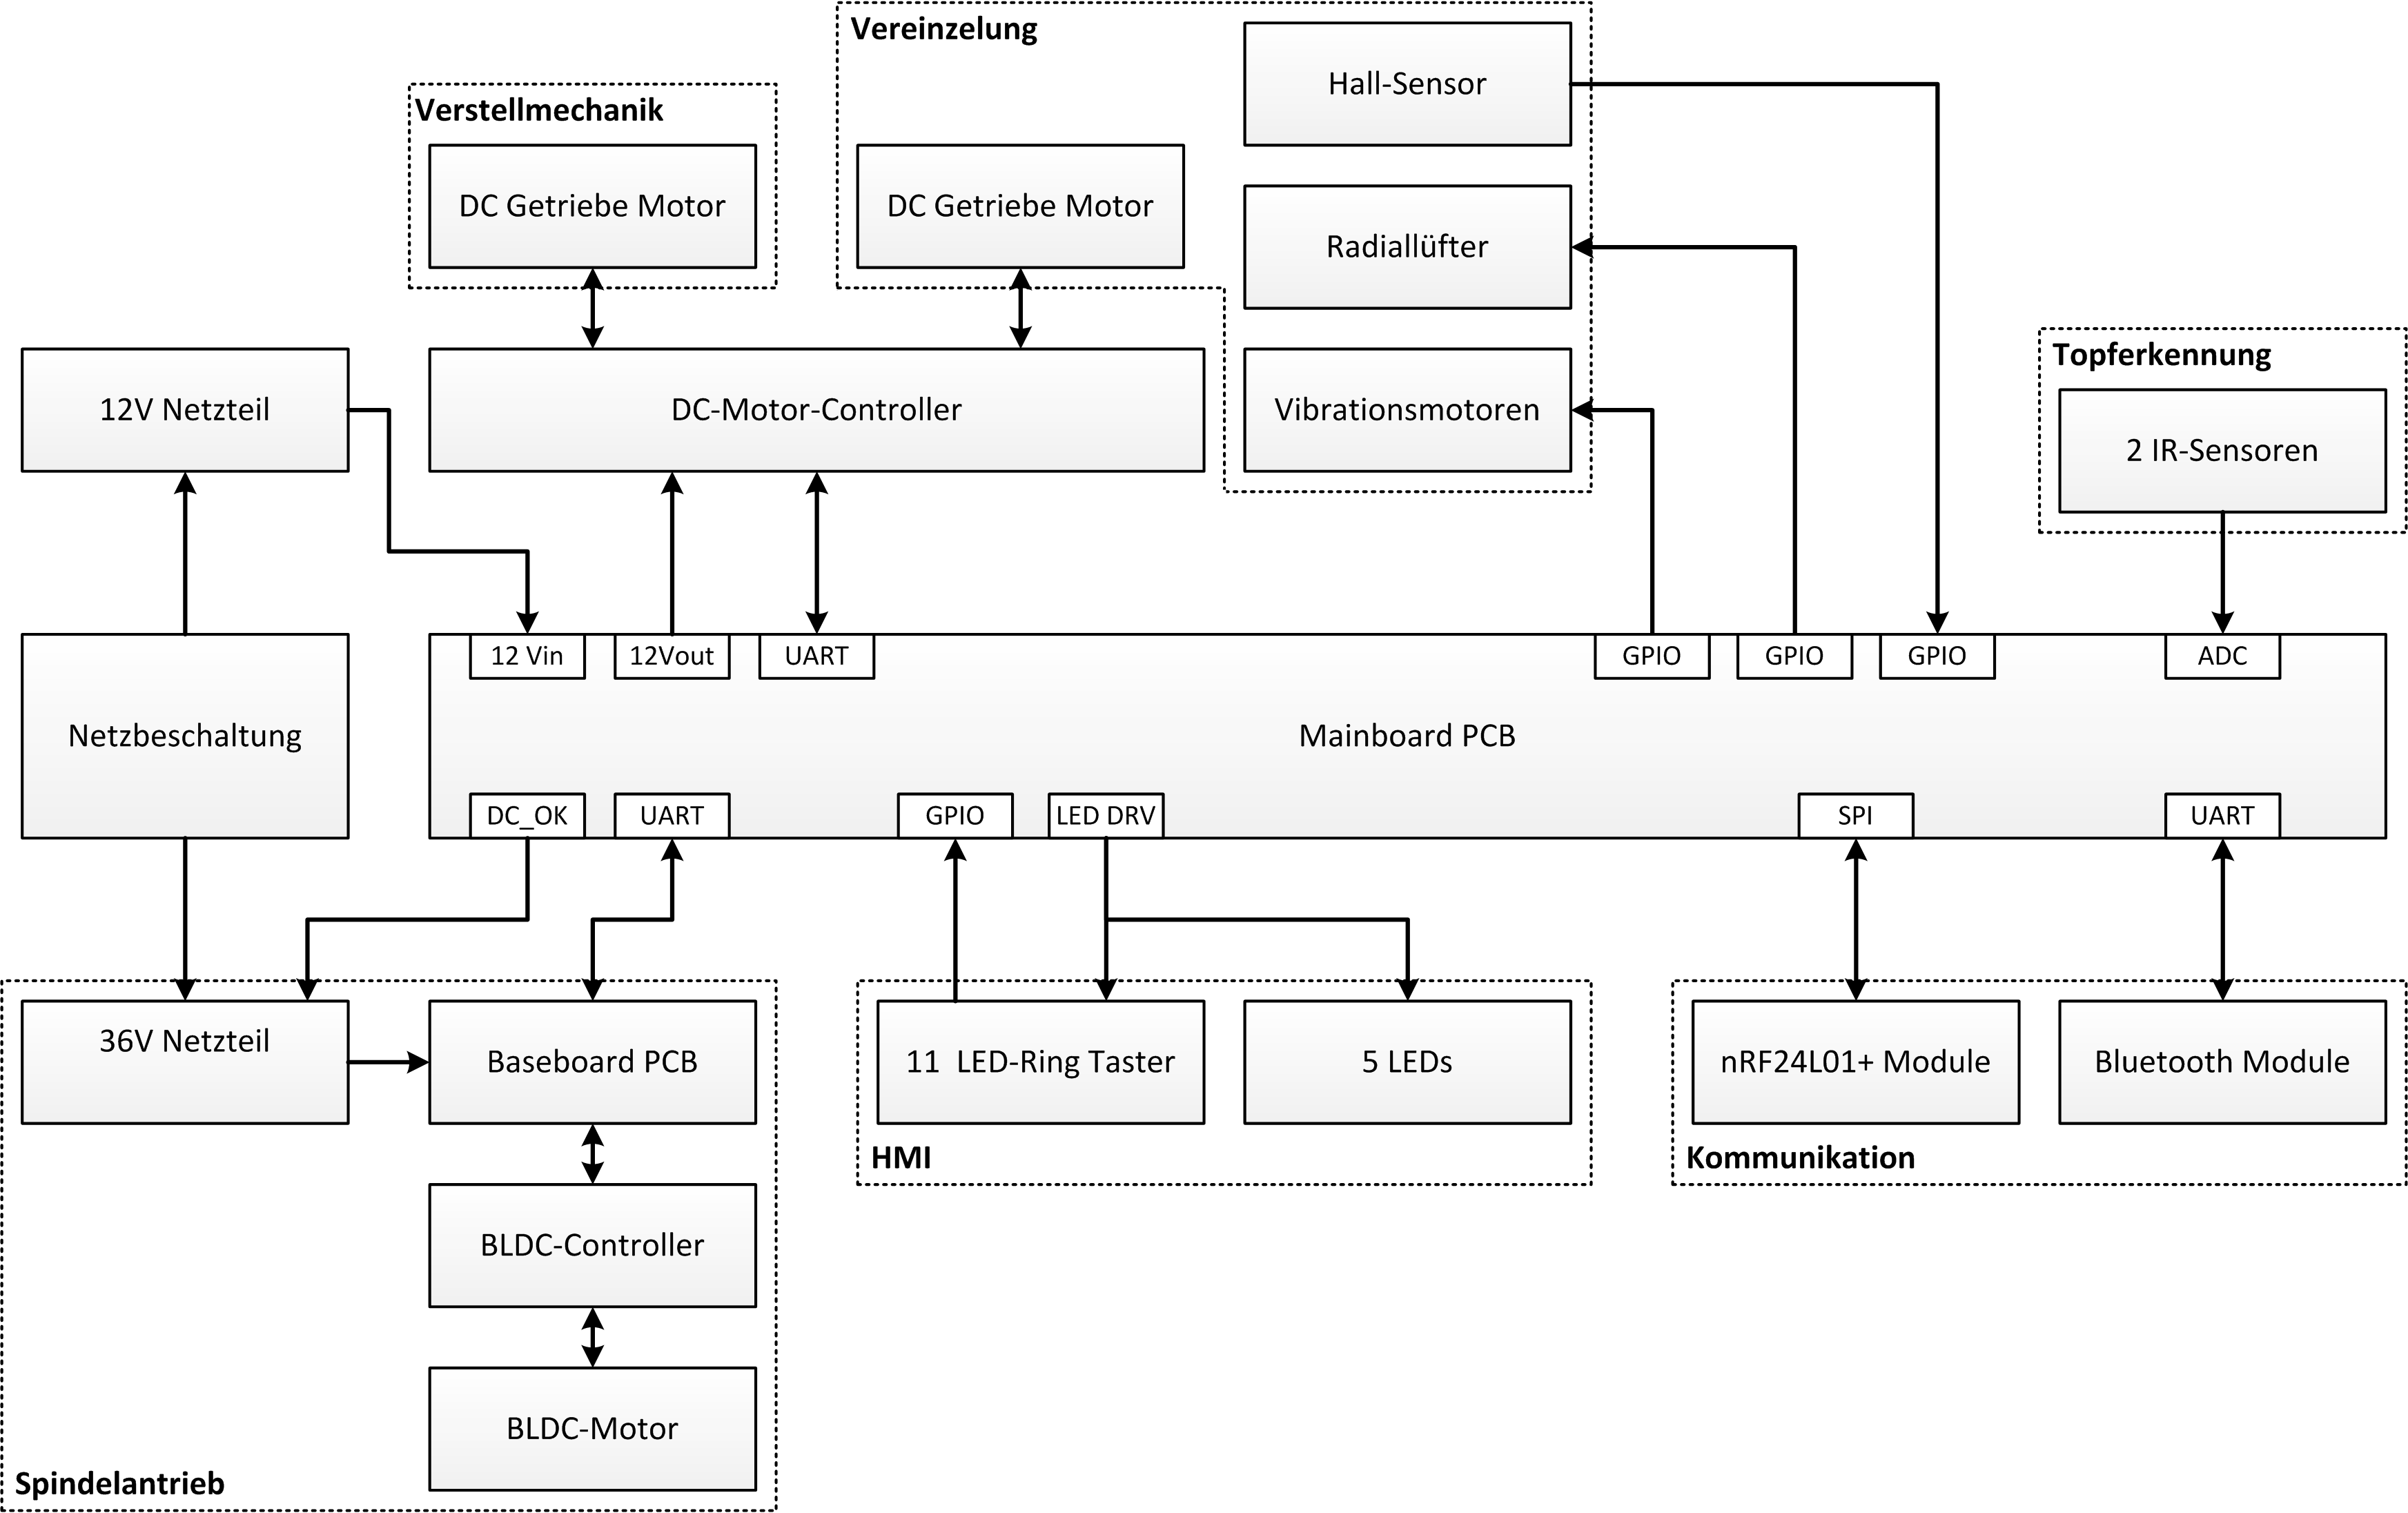
\includegraphics[width=1\textwidth]{Illustrationen/5-Konzept/Blockschaltbild_Komponenten.png}
	\caption{Blockschaltbild der Elektronik Komponenten}
	\label{fig:Blockschaltbild_Komponenten}
\end{figure}

Im folgenden Abschnitt werden die Blöcke das Blockschaltbild kurz erläutert:
\begin{itemize}
	\item \textbf{Netzbeschaltung:} Gemäss Pflichtenheft, soll der Planting Robot über 230V Netzspannung betrieben werden können. Diese Anforderung setzt eine adäquate Schutzschaltung voraus. So wurde ein Leitungsschutzschalter, sowie eine Relais Selbsthalteschaltung zum Ein und Ausschalten der Anlage über zwei Taster mit Betriebsanzeige vorgesehen. Des weiteren wurden sämtliche Gehäuseteile aus Metall, innerhalb des Schaltschrankes, mit dem Schutzleiter elektrisch verbunden.

	\item \textbf{36V Netzteil:} Um die hohe Leistungsanforderung an den Spindelantrieb bei moderatem Stromfluss erfüllen zu können, wird dessen Motor mit einem 36V Netzteil gespeist. Das FRDM-Board kann über das enable Signal des Netzteils die 36V Ausgangsspannung ein- und ausschalten.
	
	\item \textbf{Baseboard PCB:} Als Schnittstelle zwischen Mainboard PCB und BLDC-Controller dient das Baseboard PCB. Es vereinfacht die Verkabelung mit dem BLDC-Controller Board und verfügt über Drehpotentiometer zur schnellen Inbetriebnahme des BLDC-Motors.
	
	\item \textbf{BLDC-Controller:} Der BLDC-Controller wird über einen UART Port des FRDM-Boards angesteuert. Mit Hilfe der Hall-Sensor Auswertung des BLDC-Controllers kann der BLDC-Motor als Servomotor mit Positionsregelung betrieben werden. Damit kann ein Maximum an Präzision und Geschwindigkeit bei der Ansteuerung des Spindelantriebs garantiert werden.
	
	\item \textbf{Spindelantrieb:} Der Motor für den Spindelantrieb muss fähig sein die Hubspindel in sehr kurzer Zeit auf Nenndrehzahl zu beschleunigen und wieder bis zum Stillstand zu verzögern. Benötigt wird deshalb ein Motor welcher ein hohes Anlaufdrehmoment zur Verfügung stellt und häufigen Lastwechseln dauerhaft standhält. Dafür geeignet ist ein BLDC Motor mit Hall-Sensoren.
		
	\item \textbf{HMI:} Das Human-Machine Interface soll gemäss Pflichtenheft möglichst simpel gehalten werden. Es besteht deshalb aus Tastern zur Befehlseingabe und LEDs zur Statusanzeige. 
		
	\item \textbf{Topferkennung:} Die Topferkennung übernimmt zwei Funktionen. Zum einen ist sie für das Timing des Setzprozesses verantwortlich, indem sie erkennt ob sich ein Topf vor dem Planting Robot im Stillstand befindet und so bereit für den Setzprozess ist. Weiter soll sie im Umfang der Wunschanforderungen die Topfgrösse bestimmen und dementsprechend die Verstellmechanik konfigurieren können.
	
	\item \textbf{Kommunikation:} Zur Erleichterung der Inbetriebnahme sollen Parameter des Programms auf dem Mikrocontroller Board zur Laufzeit verändert werden können. Dies kann über ein Konsolenprogramm am Computer, welcher über Bluetooth mit dem Mikrocontroller Board verbunden ist, realisiert werden. Oder über das Funkmodul nRF24L01+ mit welchem ein zweites Mikrocontroller Board angesprochen werden kann.
			
	\item \textbf{12V Netzteil:} Um einen sicheren Betrieb der Elektronik während hohen Leistungsspitzen des Spindelantriebs zu garantieren, wird diese über ein separates Netzteil versorgt. Des weiteren werden auch die kleineren DC Getriebemotoren über dieses Netzteil gespeist. Das 12V Netzteil wird über das Zuschalten der Netzspannung gesteuert und kann nicht über den Mikrocontroller geschaltet werden.
	
	\item \textbf{DC-Motor-Controller:} Um die beiden DC-Getriebemotoren anzusteuern wird ein 2 Kanal Motorentreiber verwendet. Dieser ist, wie der BLDC-Controller, in der Lage mit Hilfe der Quadratur Encoder Signale der Motoren, eine Positionsregelung auszuführen. Der Treiber wird über UART angesteuert. Des weiteren befindet sich auf dem Motorcontroller eine 5V Speisung welche auf das Mainboard geführt ist. Dieses Spannungspotential wird auf dem Mainboard nur für den Antrieb von allfälligen Servos verwendet.
	
	\item \textbf{Verstellmechanik:} Die Verstellmechanik kann den Radius der Stechdornen und somit der Setzlöcher verändern. Für den Antrieb dieser Einheit kommt ein DC-Getriebemotor mit Encoder zum Einsatz. Dieser Motor wird über die Positionsregelung des DC-Motor-Controllers angesteuert. Zur absoluten Positionsbestimmung während der Initialisierung fährt der Motor an den Anschlag der Verstellmechanik bis ein definierter Laststrom erreicht wird.
	
	\item \textbf{Vereinzelung:} Die Drehscheibe der Vereinzelung wird in einer Dreh/Stopp Bewegung angetrieben. Das heisst sie dreht sich jeweils so weit bis die Löcher der Lochmasken übereinstimmen, zu diesem Zeitpunkt wird die Drehscheibe gestoppt und die Nemacaps können durch die Löcher fallen. Wie in der Verstellmechanik wird ein DC-Getriebemotor mit Encoder für den Antrieb der Vereinzelung verwendet. Zur absoluten Positionsbestimmung kommt ein Hall Sensor zum Einsatz, welcher einen Stabmagnet auf der Drehscheibe erkennt. Um allfälligen Verstopfungen der Vereinzelung vorzubeugen werden mehrere Vibrationsmotoren an der Mechanik angebracht.
	
	\item \textbf{Mainboard PCB:} Wie im Blockschaltbild dargestellt werden sämtliche Elektronikkomponenten über das selbst entwickelte Mainboard PCB miteinander verknüpft. Auf dem Mainboard PCB befindet sich das Mikrocontroller Board FRDM-KL25Z, auf welchem ein RTOS mit entsprechender Software gemäss Kap. \ref{kap:Software} implementiert ist.
\end{itemize}
\subsection{Evaluation der Komponenten}
\label{kap:Evaluation_der_Komponenten}
\subsubsection{Translation}
 	\label{subsec:Translation}

Für die Realisierung der translatorischen Bewegung der Setzeinheit bieten sich verschiedene Technologien an. In der Automatisation werden verbreitet eingesetzt:
	\begin{itemize}
	\item \textbf{Spindelantriebe:}
	Ein Motor treibt eine gelagerte Spindel an. Durch eine Bewegungsschraube wird die Rotation in eine Translation gewandelt. Spindeln sind preiswert und bieten eine hohe Gestaltungsfreiheit sowie vielfältige Einsetzbarkeit. Für Anwendungen mit hohen Geschwindigkeiten kommen Steilgewindespindeln zum Einsatz. Nachteilig ist der höhere Entwicklungsaufwand.
	\item \textbf{Elektrozylinder:}
	Elektrozylinder werden als fertige Komponenten eingekauft. In der Funktionsweise sind Elektrozylinder identisch zu Spindeln. Im Innern befindet sich auch eine Spindel, welche über einen Riemenantrieb oder Getriebe vom Motor angetrieben wird. Diese Fertigteile erreichen Geschwindigkeiten bis 600 mm/s und 15kN Axialkraft. Vrglichen mit Spindeln sind Elektrozylinder wesentlich teuerer.
	\item \textbf{Pneumatik:}
	Auch die Pneumatik bietet Lösungen für die Anwendung. Dabei wird Druckenergie in kinetische Energie gewandelt. Ein Pneumatikzylinder kann die geforderte Geschwindigkeit und Kraft für diese Anwendung aufbringen. Die einfache Implementation und Ansteuerung sind klare Vorteile. Jedoch sind Pneumatikkomponenten teuer und benötigen einen Druckluftkompressor.
	\end{itemize}

Durch den Setzprozess und die Geometrie der Töpfe sind folgende Anforderungen gegeben:
\newline
Einschaltdauer: 50 Prozent (gegeben durch Topfmaschine)
\newline
Durchschnittliche axiale Kraftaufnahme: 20N (Aus Funktionsnachweis)
\newline
Durchschnittliche Geschwindigkeit (überschlägig):
\begin{equation}
v_{avg}=\frac{2*s_{max}}{T_{min}-T_{t}}=\frac{2*100mm}{0.5s-0.1s}=500mm/s
\end{equation}

Für die Evaluation der Translation wurden alle drei Technologien unter Berücksichtigung der genannten Anforderungen in Betracht gezogen. Obwohl die Pneumatik die einfachste Umsetzung bietet, kommt diese nicht in Frage. Begründet wird dies mit dem Fehlen von Pneumatikanschlüssen in der Grundausstattung der Topfmaschine sowie den hohen Kosten.
\newline
Da zwischen Spindelantriebe und Elektrozylinder keinen funktionellen Unterschied feststellbar ist, wurde die Wahl nach Verfügbarkeit und Preis beurteilt. Im Gespräch (29.3.17) mit dem betreuenden Dozenten wurde Igus als kompetenter Hersteller von Spindeln genannt. Für Elektrozylinder wurden verschiedene Distributoren (Tecalto AG, Bachofen AG, Parkem AG, Phoenix Mecano Komponenten AG) angefragt. Nur Parkem AG konnte ein Produkt zur Offerte anbieten. Somit ergibt sich folgende Gegenüberstellung:
\begin{table}[H]
\begin{tabular}{|c|c|c|}
	\hline 
	Produkt & Igus Ds14x30 & Parkem ETH032  \\ 
	\hline 
	Typ & Spindel & Elektrozylinder \\ 
	\hline 
	Preis [CHF] & <100  & 1700    \\ 
	\hline 
	Lieferfrist [Wochen] &1 - 2  &6 \\ 
	\hline 
	Kommentar & gemäss Telefonat 5.4.17 & gemäss Mail 4.4.17 \\ 
	\hline 
\end{tabular}
	\vspace{0.2cm}
	\caption{Vergleich Spindel versus Elektrozylinder}
	\label{tab:spindelauslegung}
\end{table}
Unschwer erkennt man, dass der Preis eines Elektrozylinders um ein Vielfaches höher ist als eine Spindel. Relativieren kann man dieses Argument, wenn man bedenkt, dass für die Spindel ein Motor und die Lagerung beschafft werden muss. Entscheidend ist jedoch das zeitliche Argument. Unter Berücksichtigung des Projektplans wird rasch ersichtlich, dass eine Lieferfrist von 6 Wochen nicht mit der Umsetzung vereinbar ist. Somit wird die Translation mit einer Igus Dryspin Steilgewindespindel realisiert.



\subsection{Software}
\label{kap:Software}

\input{Kapitel/6_Umsetzung/6.0_Überblick}
\subsection{Vereinzelung} 
\label{sec:Vereinzelung}
Die Umsetzung der Vereinzelung orientiert sich stark am realisierten Funktionsnachweis. Der grundlegende Aufbau wurde beibehalten. Hinzu kommen einige Erweiterungen, um die Zuverlässigkeit und die Benutzerfreundlichkeit zu steigern.

\subsubsection{Aufbau und Funktion}
Die Vereinzelung besteht aus einer Trommel (Punkt. 1 in Abbildung \ref{fig:details_vereinzelung}), worin die NemaCaps eingefüllt werden. Durch die Rotation der Lochmaske (3), welche durch einen Getriebemotor (7) umgesetzt wird, fallen die NemaCaps in die vorgesehenen Löcher . Überschüssige NemaCaps werden durch mehrere Bürsten (6) abgestreift. Sobald die vereinzelten NemaCaps bei den Schlauchkupplungen (8) angekommen sind, sollen diese durch die Schläuche zur Einsetzlokalität fallen. Alle Komponenten werden auf einer Grundplatte (4) montiert, wobei diese in ihrer Neigung verstellbar gelagert ist.
	\begin{figure}[H]
	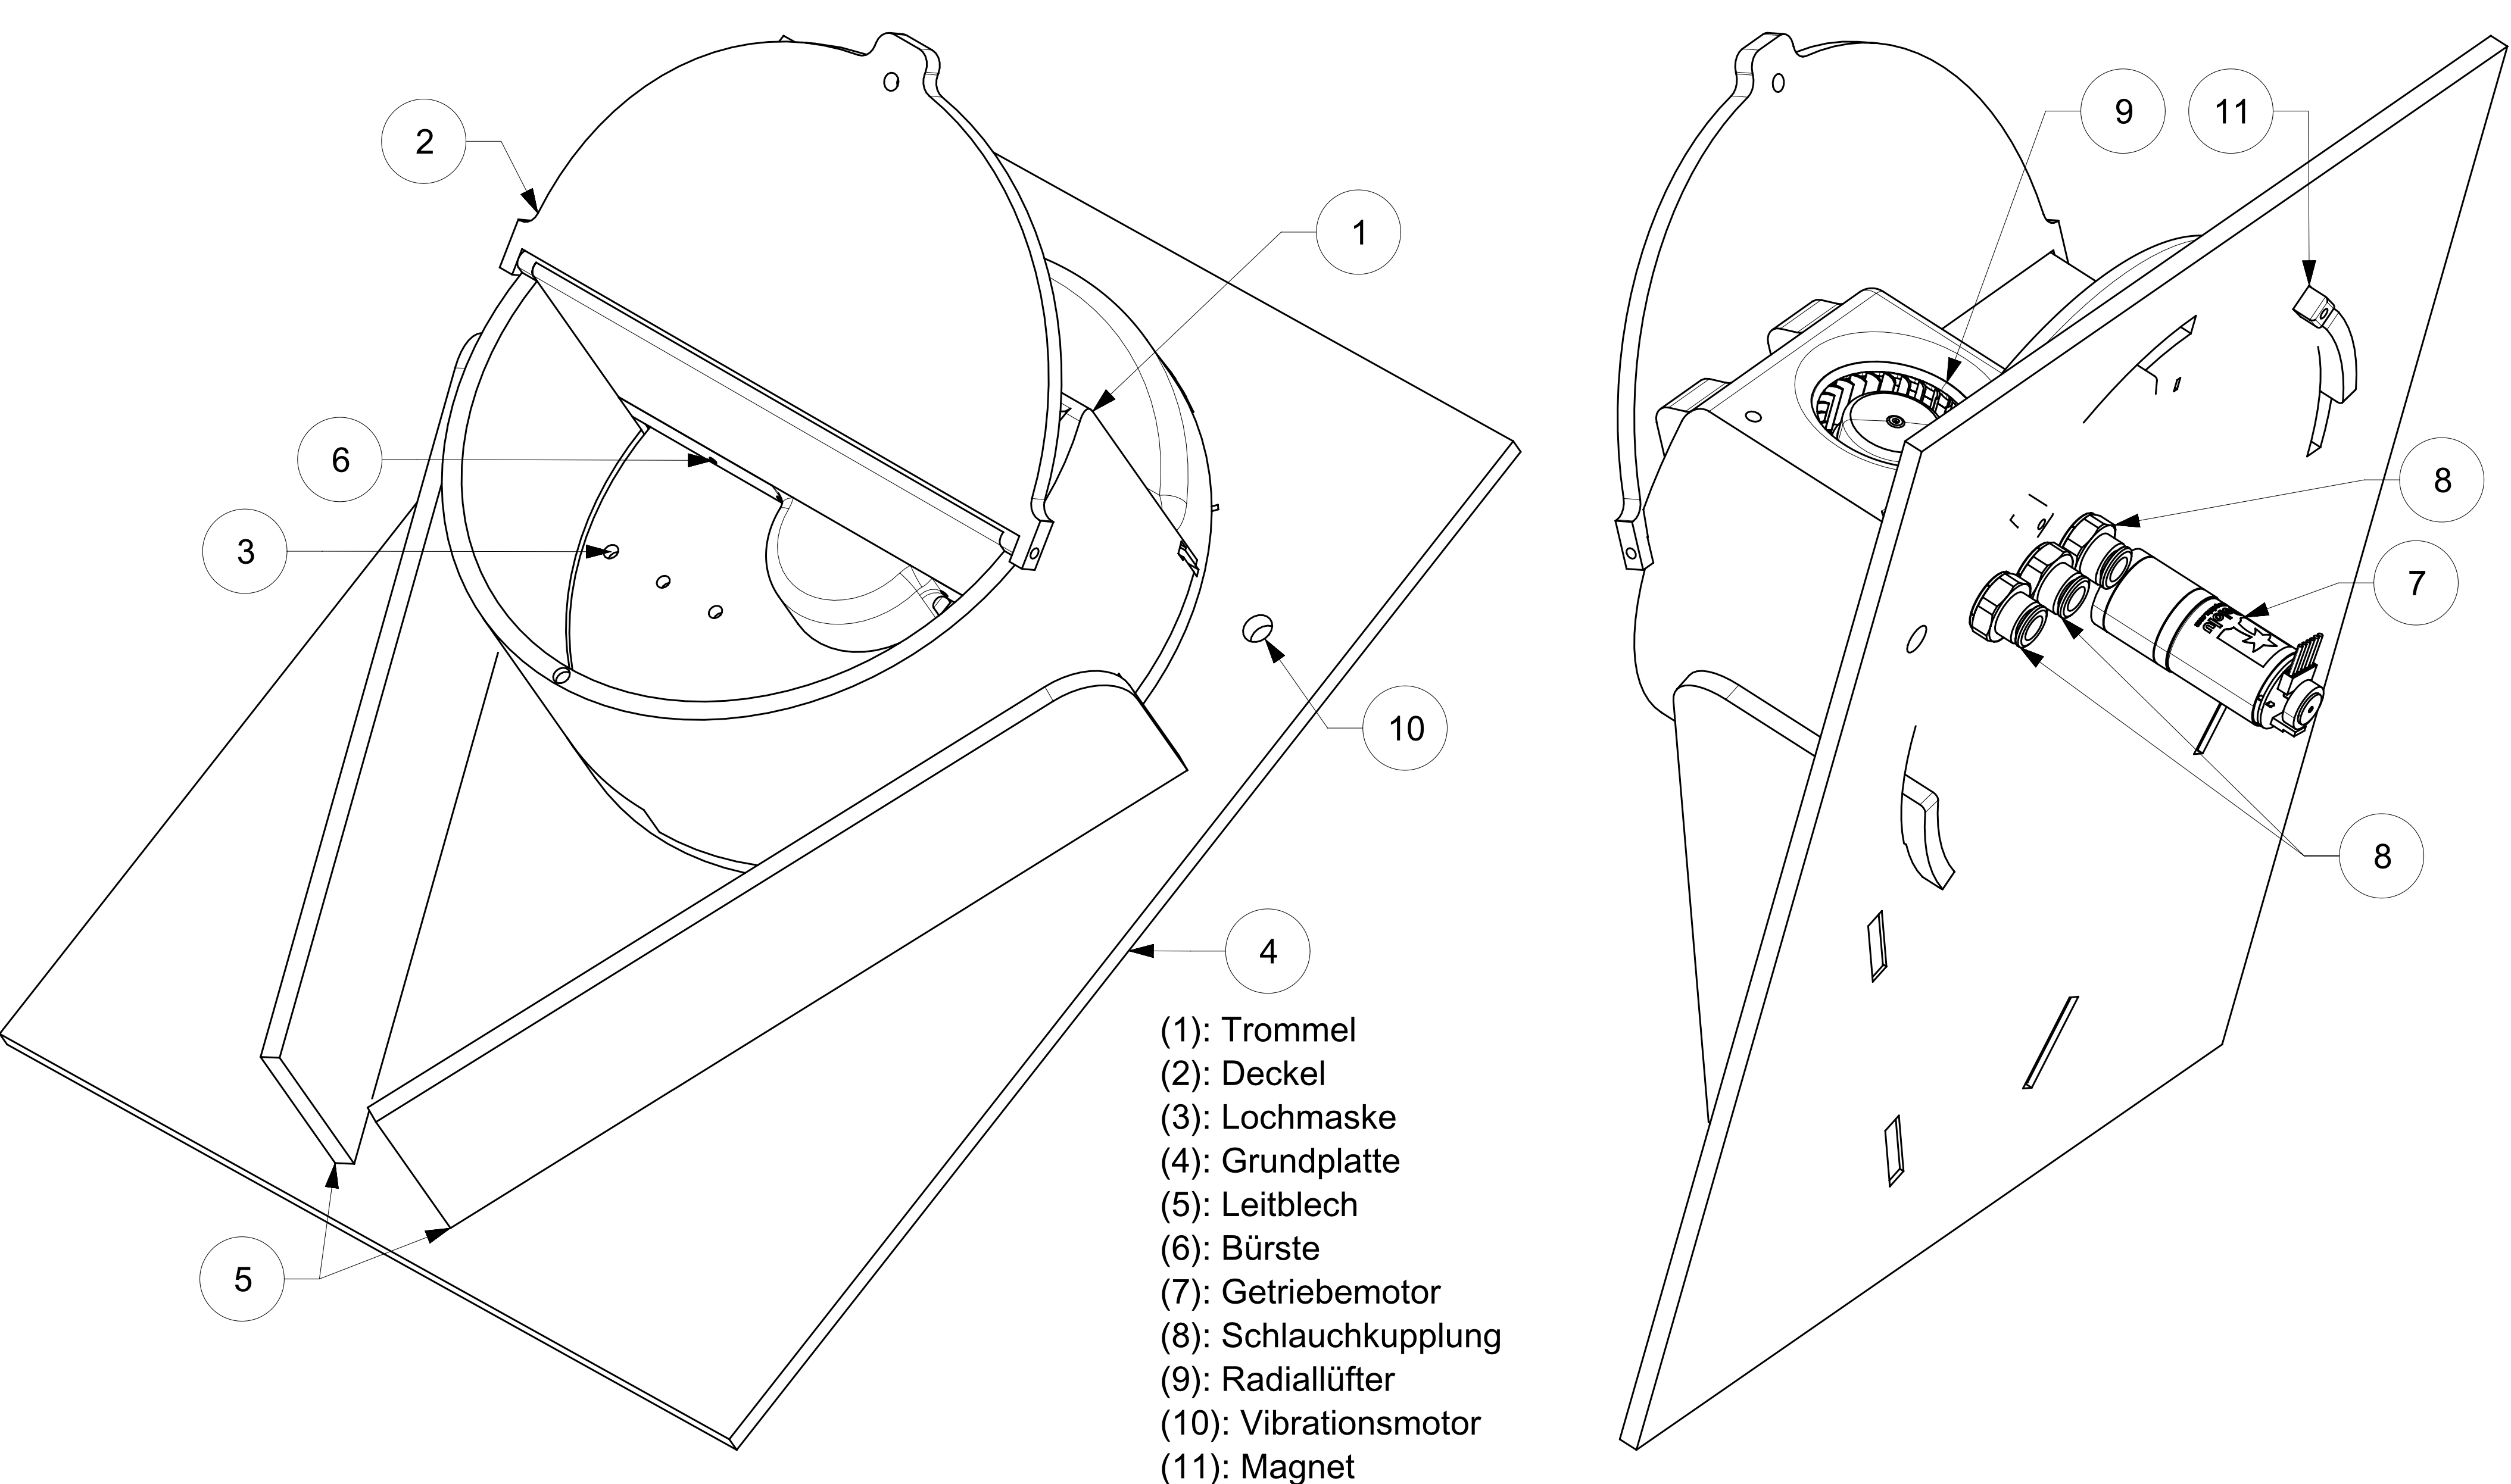
\includegraphics[scale=0.455]{Illustrationen/6-Umsetzung/details_vereinzelung.jpg}
	\caption{Detaillierte Übersicht der Vereinzelung}
	\label{fig:details_vereinzelung}
	\end{figure}

\subsubsection{Abhilfemassnahmen}
\label{abhilfe}
Der Funktionsnachweis aus Kapitel \ref{funktionsnachweis} zeigte auf, dass Komplikationen auftreten können. In erschwerten Bedingungen, wie nassem Pulver, kann das NemaCap  durch die erhöhte Adhäsion an der Lochmaske hängen bleiben. So wurde im Funktionsnachweis die Bedingung formuliert, dass eine Umsetzung dieser Funktion nur mit konkreten Abhilfemassnahmen umgesetzt werden darf, um die Zuverlässigkeit der Vereinzelung zu steigern. Diese sind:
\begin{itemize}
	\item \textbf{Vibrationsmotor:} Der Funktionsnachweis zeigte, dass durch leichtes Klopfen an der Einheit, hängengebliebene NemaCaps erfolgreich gelöst werden. Somit wird in der Nähe der Schlauchkupplungen ein Vibrationsmotor (Punkt. 10 in Abbildung \ref{fig:details_vereinzelung}) angebracht, welche die Einheit in Schwingung bringen soll. Wichtig ist die Grundplatte in einer Richtung federnd zu lagern, sodass diese tatsächlich in Schwingung geraten kann.

	
	\item \textbf{Radiallüfter:} Eine weitere Möglichkeit die NemaCaps zu lösen, bietet ein gezielter Luftstoss. Daher ist in der Trommel ein Radiallüfter (9) integriert, welcher einen Luftstrom auf die vereinzelten NemaCaps in der Lochmaske richtet. Bei Bedarf werden zusätzliche Löcher an den Schläuchen angebracht, um den Luftaustritt zu verbessern. 
	
	\item \textbf{Lochmaske:} Am Funktionsnachweis wurde ersichtlich, wie kritisch die Materialwahl sowie Fertigungsqualität der Lochmaske ist. Die formulierten Punkte zur Steigerung der Zuverlässigkeit sind im Kapitel \ref{lochmaske} erläutert.
\end{itemize}

\subsubsection{Handhabung}
Die Verwendung von frischen NemaCaps trägt zur verbesserten Zuverlässigkeit der Vereinzelung bei. Der benutzerfreundliche Wechsel von NemaCaps ist also ein wichtiges Anliegen und wird in der Konstruktion der Vereinzelung berücksichtigt. So ist die Trommel (Punkt 1 in Abb. \ref{fig:vereinzelung_entleeren}) mit einem dreifachen Bajonettverschluss (Detail C in Abb. \ref{fig:vereinzelung_entleeren} und Punkt 12 in Abb. \ref{fig:details_vereinzelung}) versehen. Die Trommel kann mit einer Drehung von 15° im Gegenuhrzeigersinn entriegelt werden (Detail A in Abb. \ref{fig:vereinzelung_entleeren}). Nun kann die Trommel entfernt werden (Detail B). Die verbleibenden NemaCaps (Detail X) rollen nun auf der Grundplatte hinunter. Geleitet durch zwei Leitbleche (5) fallen diese in Richtung Detail Y, wo man diese in einem Behälter sammeln kann. Auch verfügt die Trommel über einen Deckel (2), welcher durch zwei angebrachte Magnete sicher verschlossen wird.
	\begin{figure}[H]
	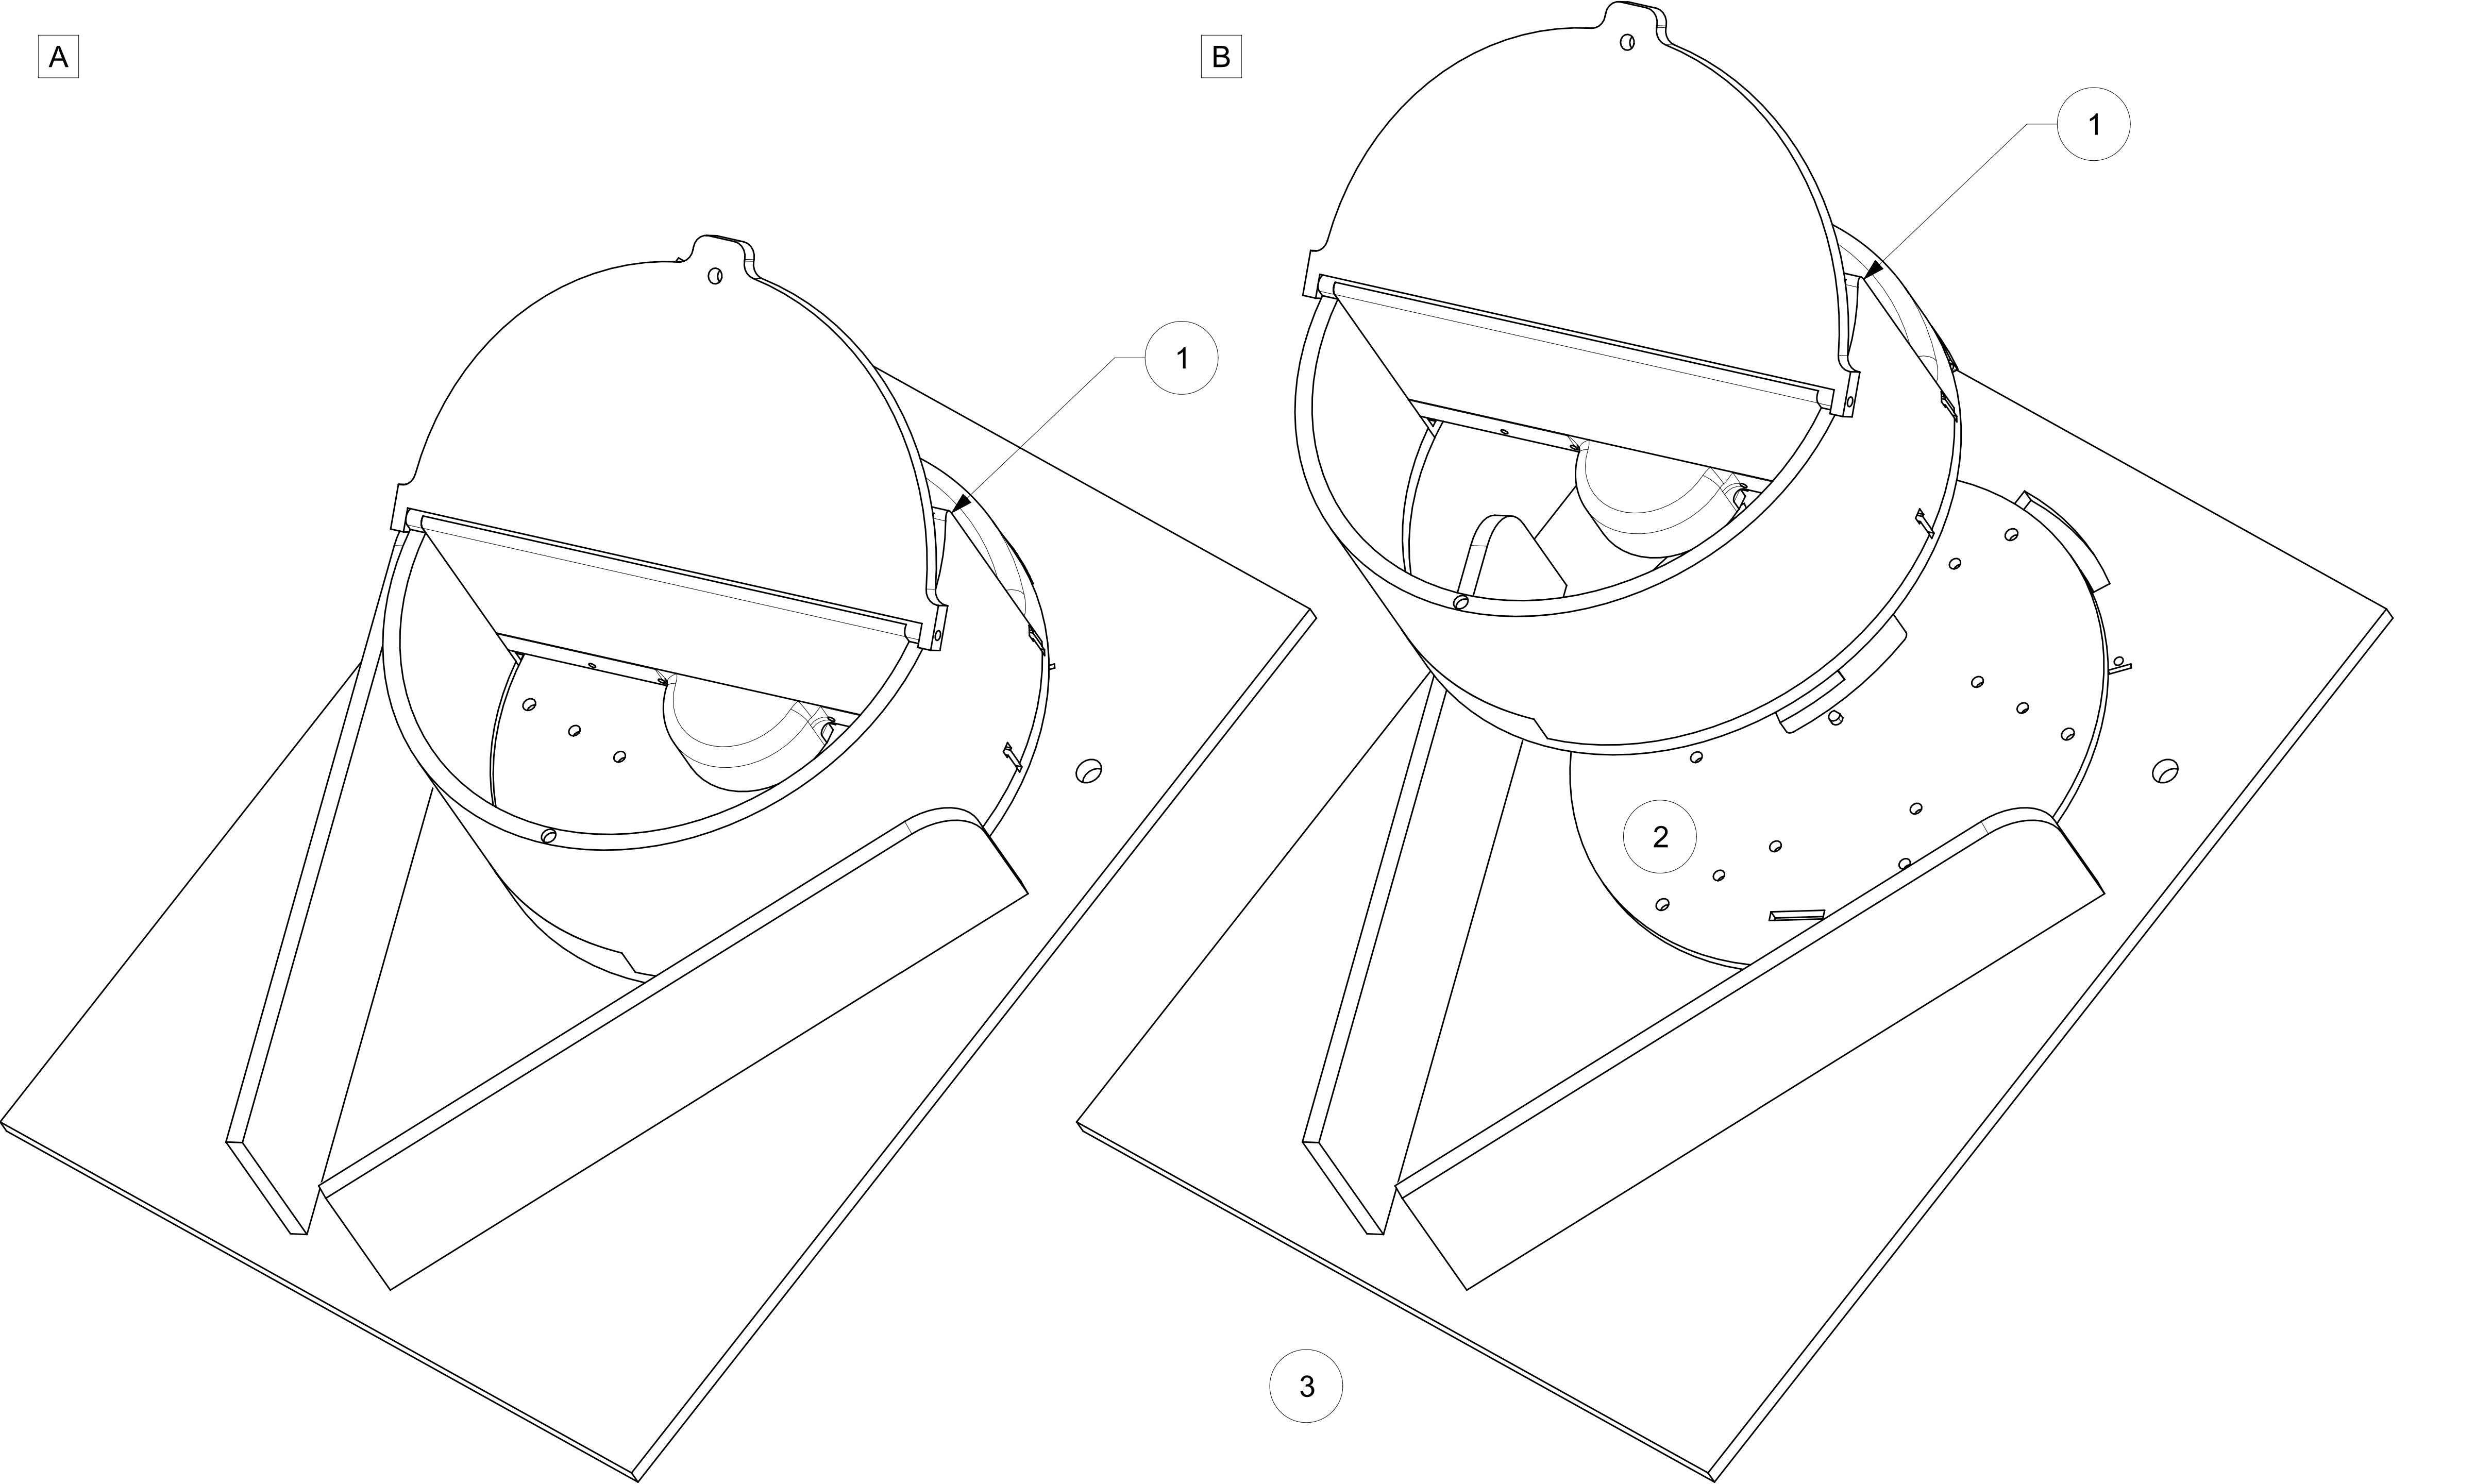
\includegraphics[scale=0.42]{Illustrationen/6-Umsetzung/vereinzelung_entleeren.jpg}
	\caption{Entleerung der Trommel}
	\label{fig:vereinzelung_entleeren}
	\end{figure}
\subsubsection{Lochmaske}
\label{lochmaske}
Der Funktionsnachweis hat gezeigt, dass das Scheitern der Vereinzelung meist durch das Hängenbleiben der NemaCaps an der Lochmaske verursacht wird. Die Zuverlässigkeit dieser Funktion hängt direkt von den Eigenschaften der Lochmaske ab. Die Materialwahl sowie Fertigungsqualität von diesem Teil ist entscheidend. 
\newline
Folgende Massnahmen werden umgesetzt:
\begin{itemize}
	\item \textbf{Materialwahl:} Die Wahl des passenden Materials mit der geringsten Adhäsion wurde mittels praktischen Tests am 26.4.2017 durchgeführt. Dabei wurden gängige laserbare Materialien (Aluminium, Plexiglas und MDF) miteinander verglichen. Die Tests zeigen, dass Aluminium die geringste Adhäsion gegenüber von NemaCaps aufweist, gefolgt von Plexiglas. Mit MDF wurde die grösste Adhäsion festgestellt, was sich durch die erhöhte Pulveraufnahme und die rauhere Oberfläche erklären lässt. 
	Die höchste Zufriedenstellung wird mit Aluminium erreicht, wobei die Reibung zwischen Lochmaske und Grundplatte noch nicht berücksichtigt ist. Bei zu hoher Reibung kann auf Plexiglas ausgewichen werden.
	
	\item \textbf{Fertigungsqualität:} Die Tests vom 26.4.2017 zeigten auch, dass die Rauheit der Oberfläche relevant ist. Je feiner die Oberfläche der Bohrung (Punkt 13 in Abbildung \ref{fig:detail_lochmaske}), desto geringer das Risiko, dass NemaCaps hängenbleiben. Folglich werden diese Löcher nach der Bohrung zusätzlich mit einer Reibale (\textbf{H7?}) ausgerieben. Der ideale Durchmesser D1 muss während der Inbetriebnahme durch zielgerichtetes Ausprobieren erörtert werden.
	
\end{itemize}
Desweiteren ist die Lochmaske mit zwei Langlöchern (14) ausgestattet. Diese werden zur Einpassung von Dauermagneten verwendet, welche zur Positionsbestimmung der Lochmaske dienen. Der Abstand B in Abbildung \ref{fig:detail_lochmaske} ist gegeben durch die Grösse der Schlauchkupplungen (Punkt 8 in Abb. \ref{fig:details_vereinzelung}) und kann dadurch nicht verkleinert werden \cite{camozzi2}.
	\begin{figure}[H]
	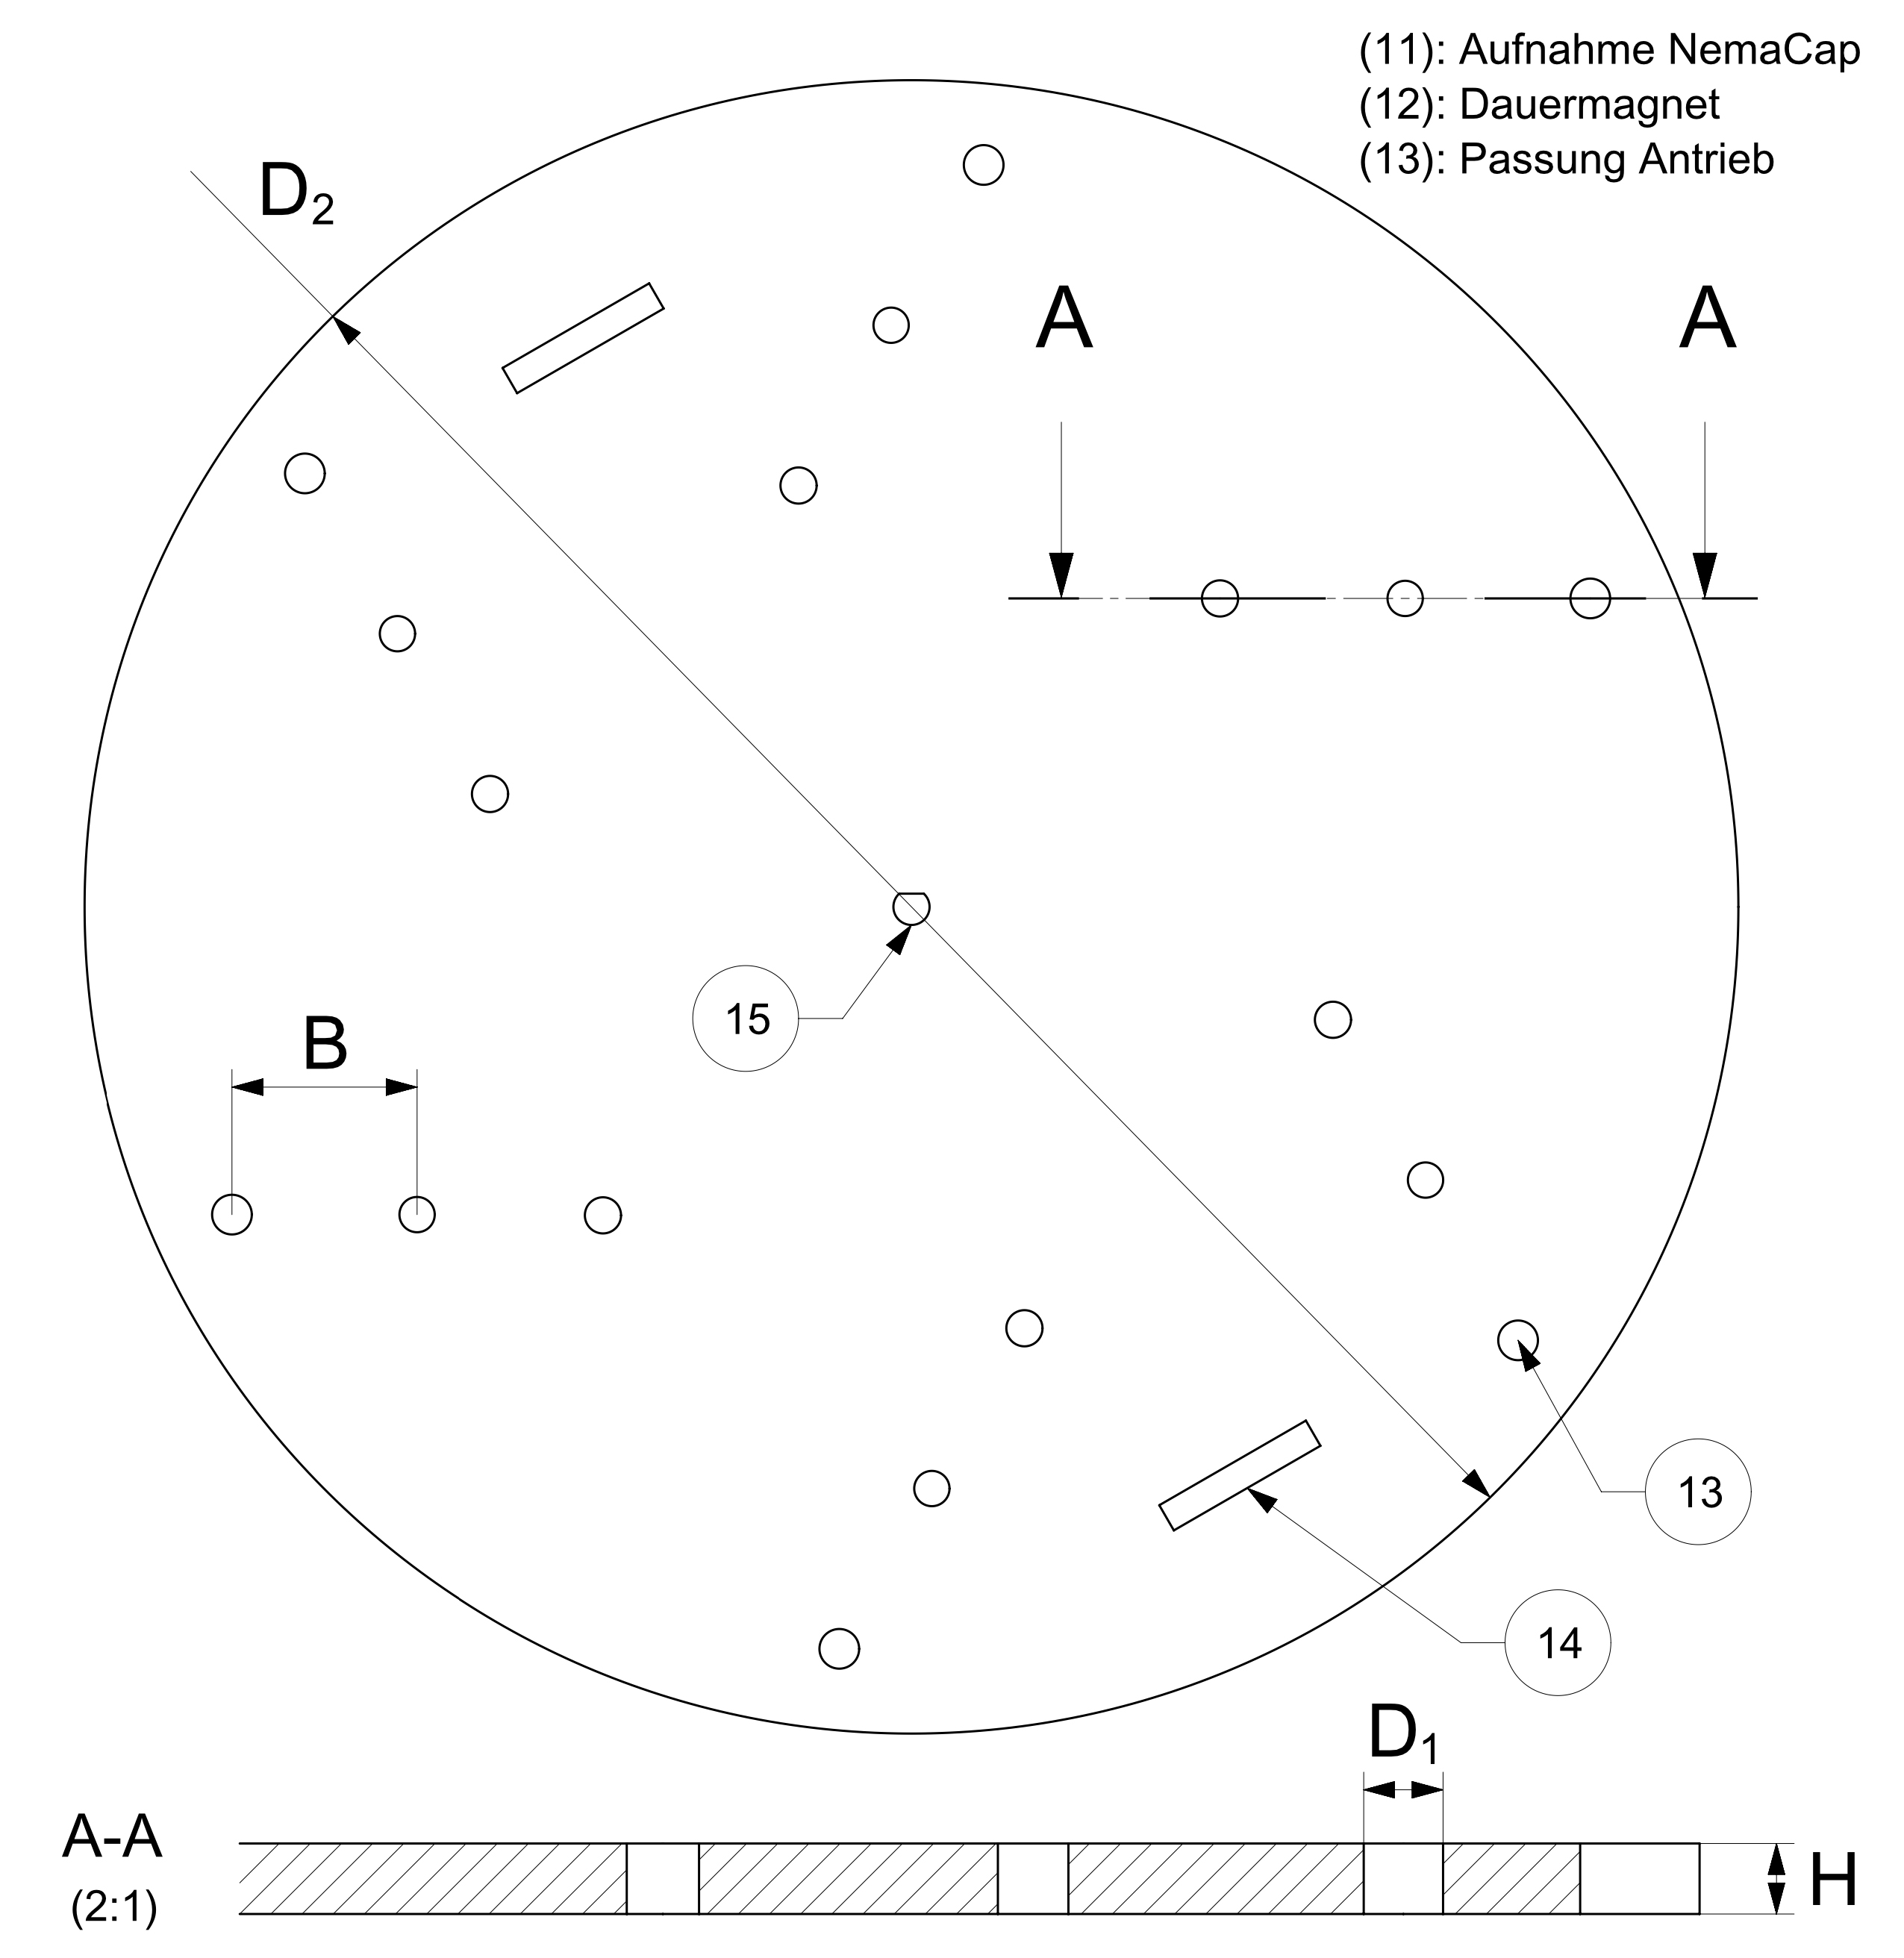
\includegraphics[scale=0.75]{Illustrationen/6-Umsetzung/detail_lochmaske.jpg}
	\caption{Grundriss der Lochmaske mit Schnitt}
	\label{fig:detail_lochmaske}
	\end{figure}

\subsubsection{Prozessablauf}
\textit{(pro)} Die Vereinzelung benötigt einen drehmomentstarken Antrieb um eine flüssige Funktion zu gewährleisten. Dafür wird ein DC Getriebemotor von Pololu mit einer Getriebeübersetzung von 99:1 verwendet. Die Spezifikationen, sowie die Begründung für die Wahl dieser Antriebstechnik sind in Kapitel \ref{kap:Evaluation_der_Komponenten} erläutert.
\\ Um die Lochmaske präzise positionieren zu können, kommen zwei Sensorik Systeme zum Einsatz. Ein Hall Sensor zur absoluten Bestimmung der Position der Lochmaske, sowie der Quadratur Encoder des Motors zur Bestimmung des zurückgelegten Winkels, relativ zur gemessenen Position. Es wird der digitale Hall Sensor SS441A von Honeywell verwendet (siehe Abb. \ref{fig:SS441A}). Das Bauteil kann mit einer Spannung von 3.8V bis 30V betrieben werden. Die typische Stromaufnahme beläuft sich dabei bei einer Spannung von 5V auf 6.5mA. Der Hall Sensor reagiert auf den Südpol des verwendeten Stabmagneten und löst bei Raumtemperatur ab einem magnetischen Feld von 55G aus.

\begin{figure}[H]
	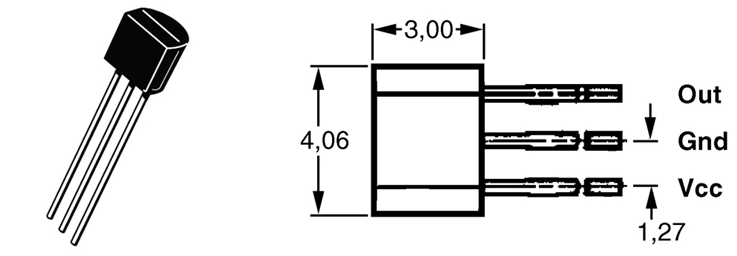
\includegraphics[width=0.9\textwidth]{Illustrationen/6-Umsetzung/Hall_Sensor.png}
	\caption{SS441A, digitaler Hall Sensor \protect\cite{SS441A}}
	\label{fig:SS441A}
\end{figure}

Das System initialisiert sich nach einem Neustart einmalig und ist dann für den Betrieb bereit. Der ganze Prozess der Vereinzelung ist in Abb. \ref{fig:Ansteuerung_Vereinzelung} illustriert.  Der Prozess wurde dabei in vier Etappen unterteilt welche mit den Ziffern 1... 4 nummeriert sind.

\begin{figure}[H]
	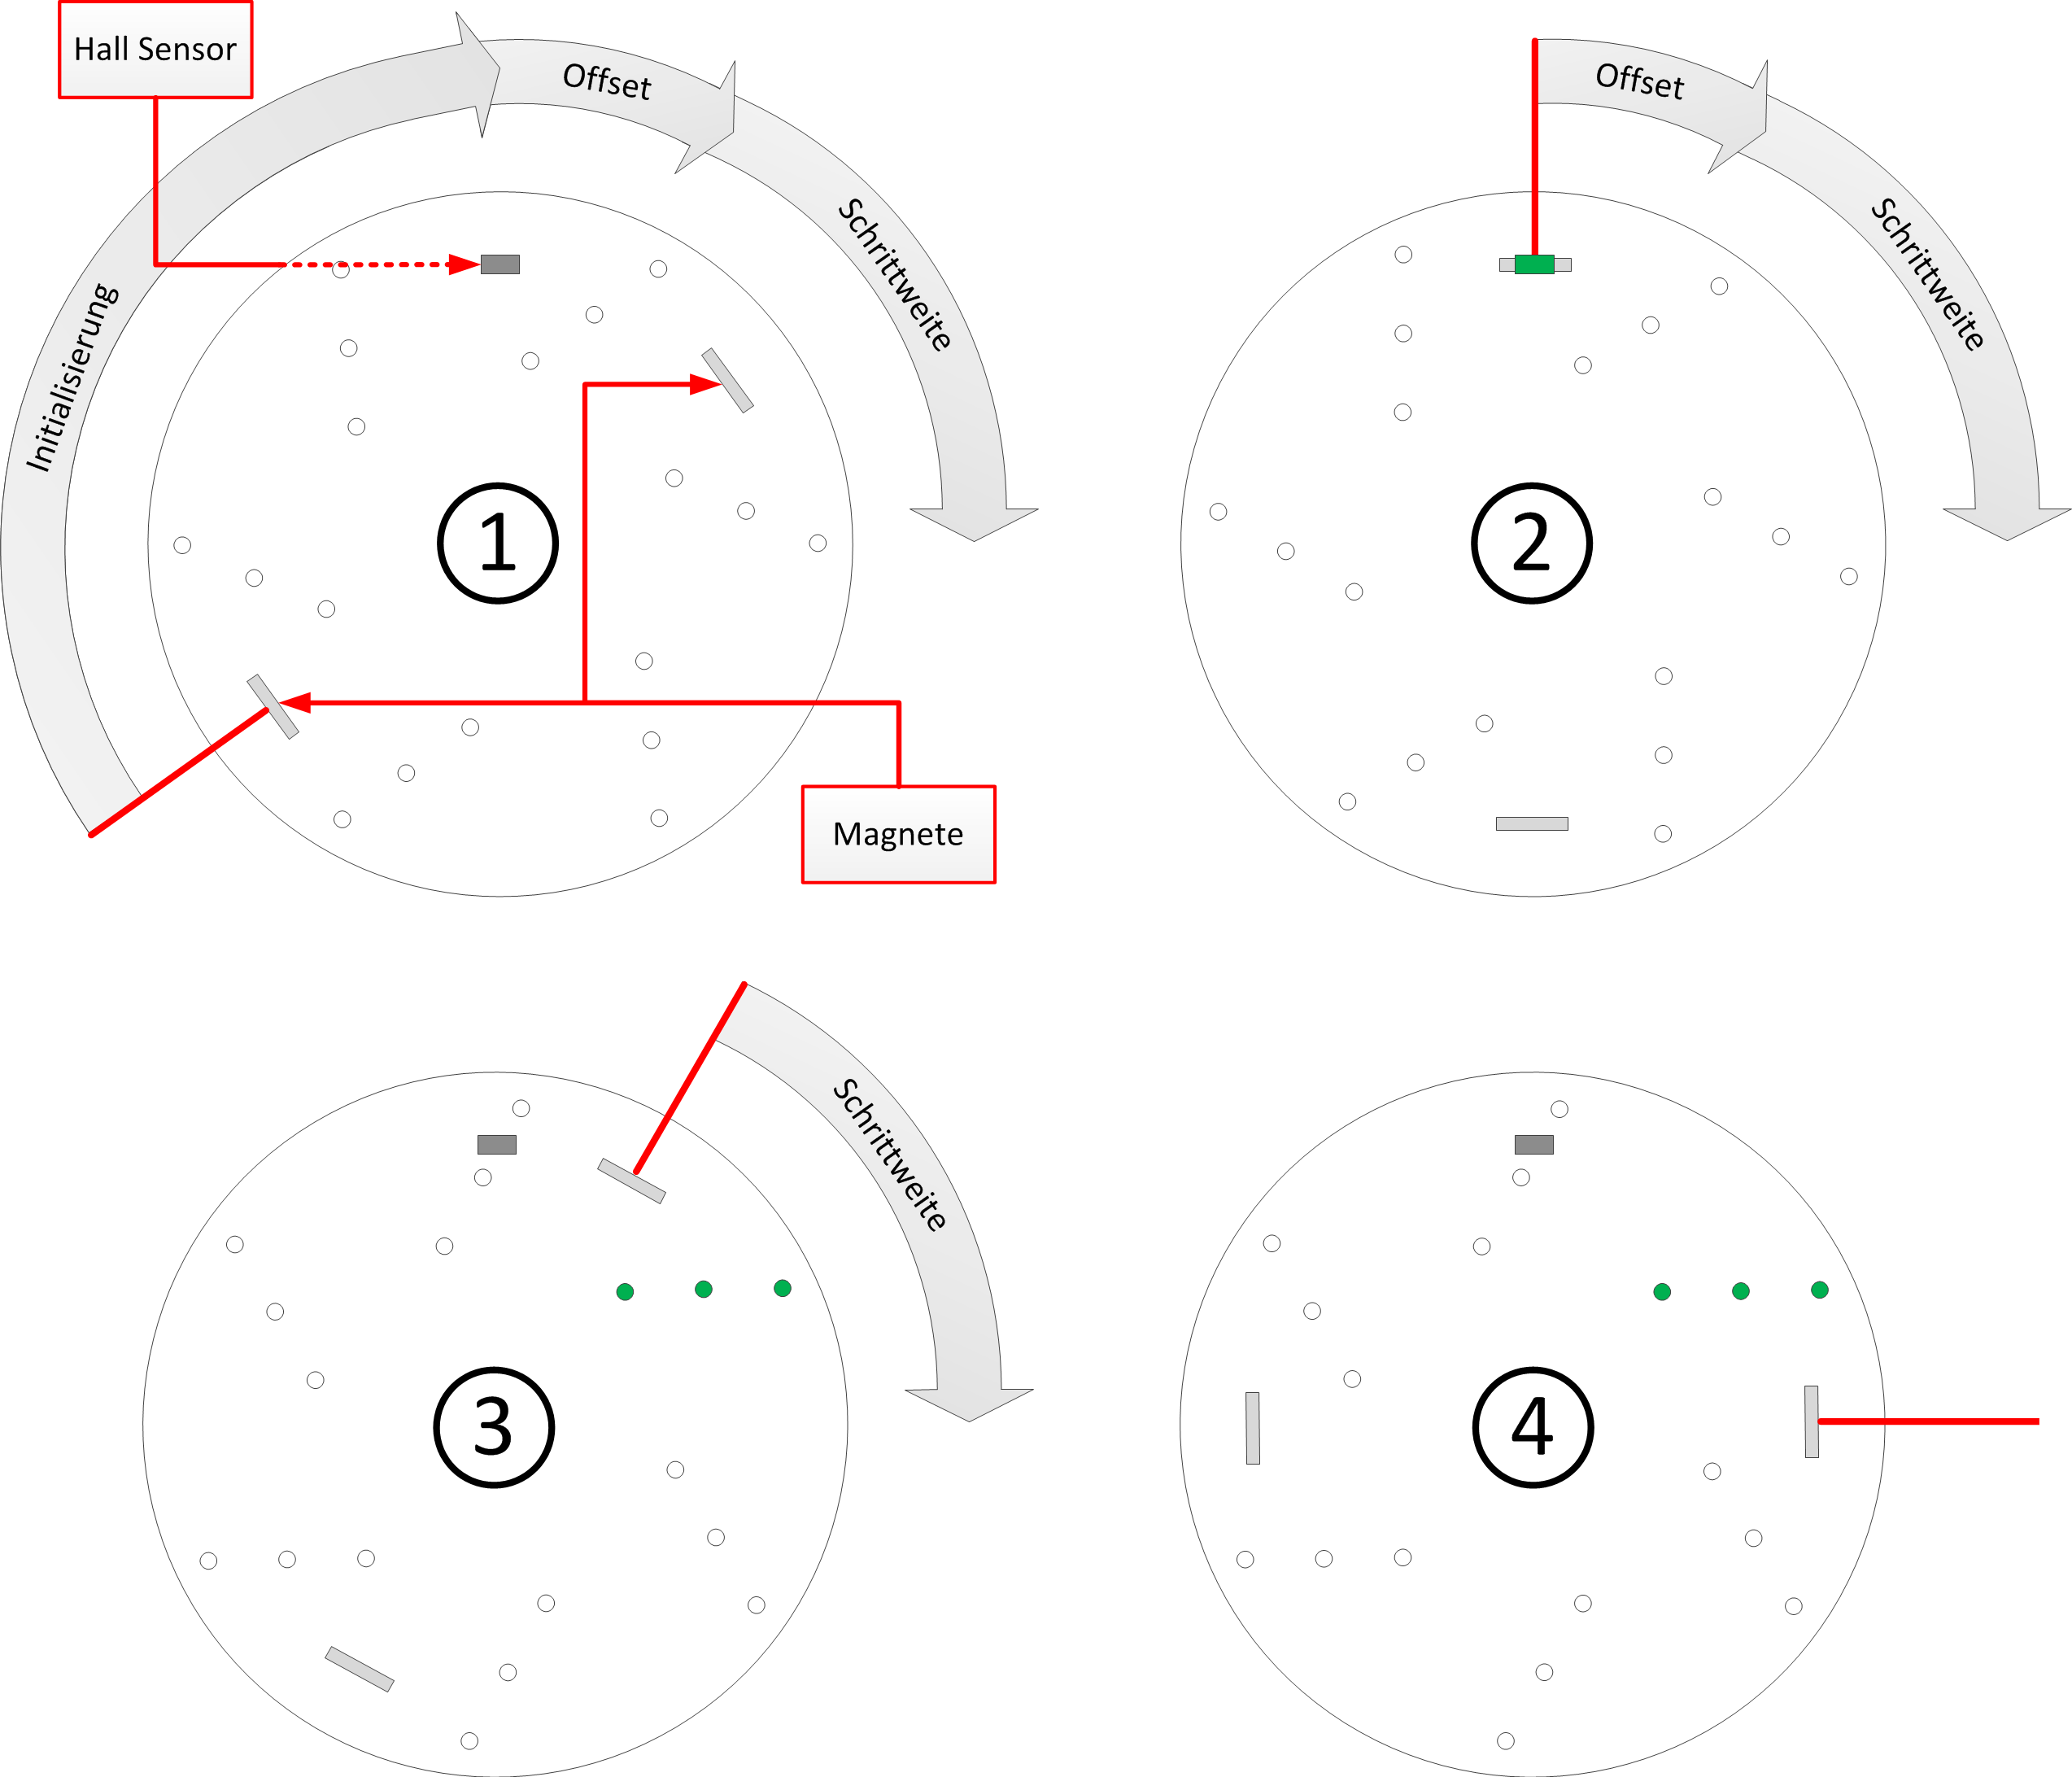
\includegraphics[width=0.9\textwidth]{Illustrationen/6-Umsetzung/Prozessablauf_Vereinzelung.png}
	\caption{Prozessablauf der Vereinzelung}
	\label{fig:Ansteuerung_Vereinzelung}
\end{figure}

Im folgenden Abschnitt werden die vier Etappen erläutert:

\begin{enumerate}
	\item Die Lochmaske wird solange gedreht bis einer der beiden Permanentmagnete, welche sich mit der Lochmaske drehen, den Hall Sensor erreichen. Der Hall Sensor ist fest hinter der Lochmaske montiert.
 	\item Zu diesem Zeitpunkt hat ein Magnet den Hall Sensor erreicht. Die Lochmaske wird eine definierte Anzahl Encoder Counts (Offset) weiter gedreht, bis die Löcher der Lochmasken übereinstimmen.
 	\item Das System ist nun initialisiert und bereit für den Betrieb. In dieser Etappe der Vereinzelung stimmen die Löcher der Lochmaske überein und die Nemacaps fallen durch die Lochmaske. 
	\item Die Nemacaps werden nun durch drehen der Lochmaske mit einer definierten Anzahl Encoder Counts (Schrittweite) repetitiv ausgelöst.
\end{enumerate}

Auch nach der Initialisierungsphase wird jedes mal wenn ein Magnet den Hall Sensor erreicht, die Position der Lochmaske neu ermittelt. Dadurch wird eine mögliche Ungenauigkeit durch aufaddieren der Fehler in der Schrittweite vermieden. Ausserdem wird dadurch der Fehler durch mögliche Impulsverluste minimiert. Die Parametrisierung des Prozessablaufs wird im Kapitel Inbetriebnahme (\ref{sec:Inbetriebnahme_Vereinzelung}) behandelt. 
\subsection{Setzeinheit} \label{sec:Setzeinheit}
\textit{(ygu)} Die Setzeinheit bezeichnet alle Teile, welche durch die Translation bewegt werden. Auch zur Setzeinheit gehören die Spindel sowie der Spindelantrieb, welche die Translation umsetzen.
\newline
Die wesentlichen Komponenten der Setzeinheit sind in Abbildung \ref{fig:setzeinheit} dargestellt. Dabei wird in diesem Unterkapitel ausschliesslich auf die Komponenten der Setzeinheit eingegangen. Alle Komponenten die zur Verstellung des Topfradius dienen, sind in der Abb.  \ref{fig:setzeinheit} unter Punkt 8 (Verstellmechanik) gesammelt und werden im Kapitel \ref{verstellmechanik} näher erläutert.
\newline

\subsubsection{Aufbau}
Die Spindel ist durch eine bewegte Montageplatte (Punkt. 16 in Abb. \ref{fig:setzeinheit}) und drei Führungen (6) mit der Verstellmechanik (8) verbunden. Diese Führungen werden durch drei Gleitlager (7)  an einer Montageplatte (14) gelagert. die zwei oberen Montageplatten (12, 13) dienen zur Montage des Spindelantriebes sowie zur Lagerung der Spindel (4). Um eine weitere Montageplatte zu sparen, ist der Spindelantrieb mittels einer Distanzhülse (2) mit der obersten Montageplatte (12) verbunden. Die unterste Montageplatte (15) dient zur Lagerung der Verstellmechanik sowie zum einfachen Schutz der Mechanik vor Topferde. Dadurch ist gewährleistet, dass nur ein minimaler Teil (der Stechdorn, 9 - 11) der bewegten Komponenten in Kontakt mit der Topferde kommt.
	\begin{figure}[H]
	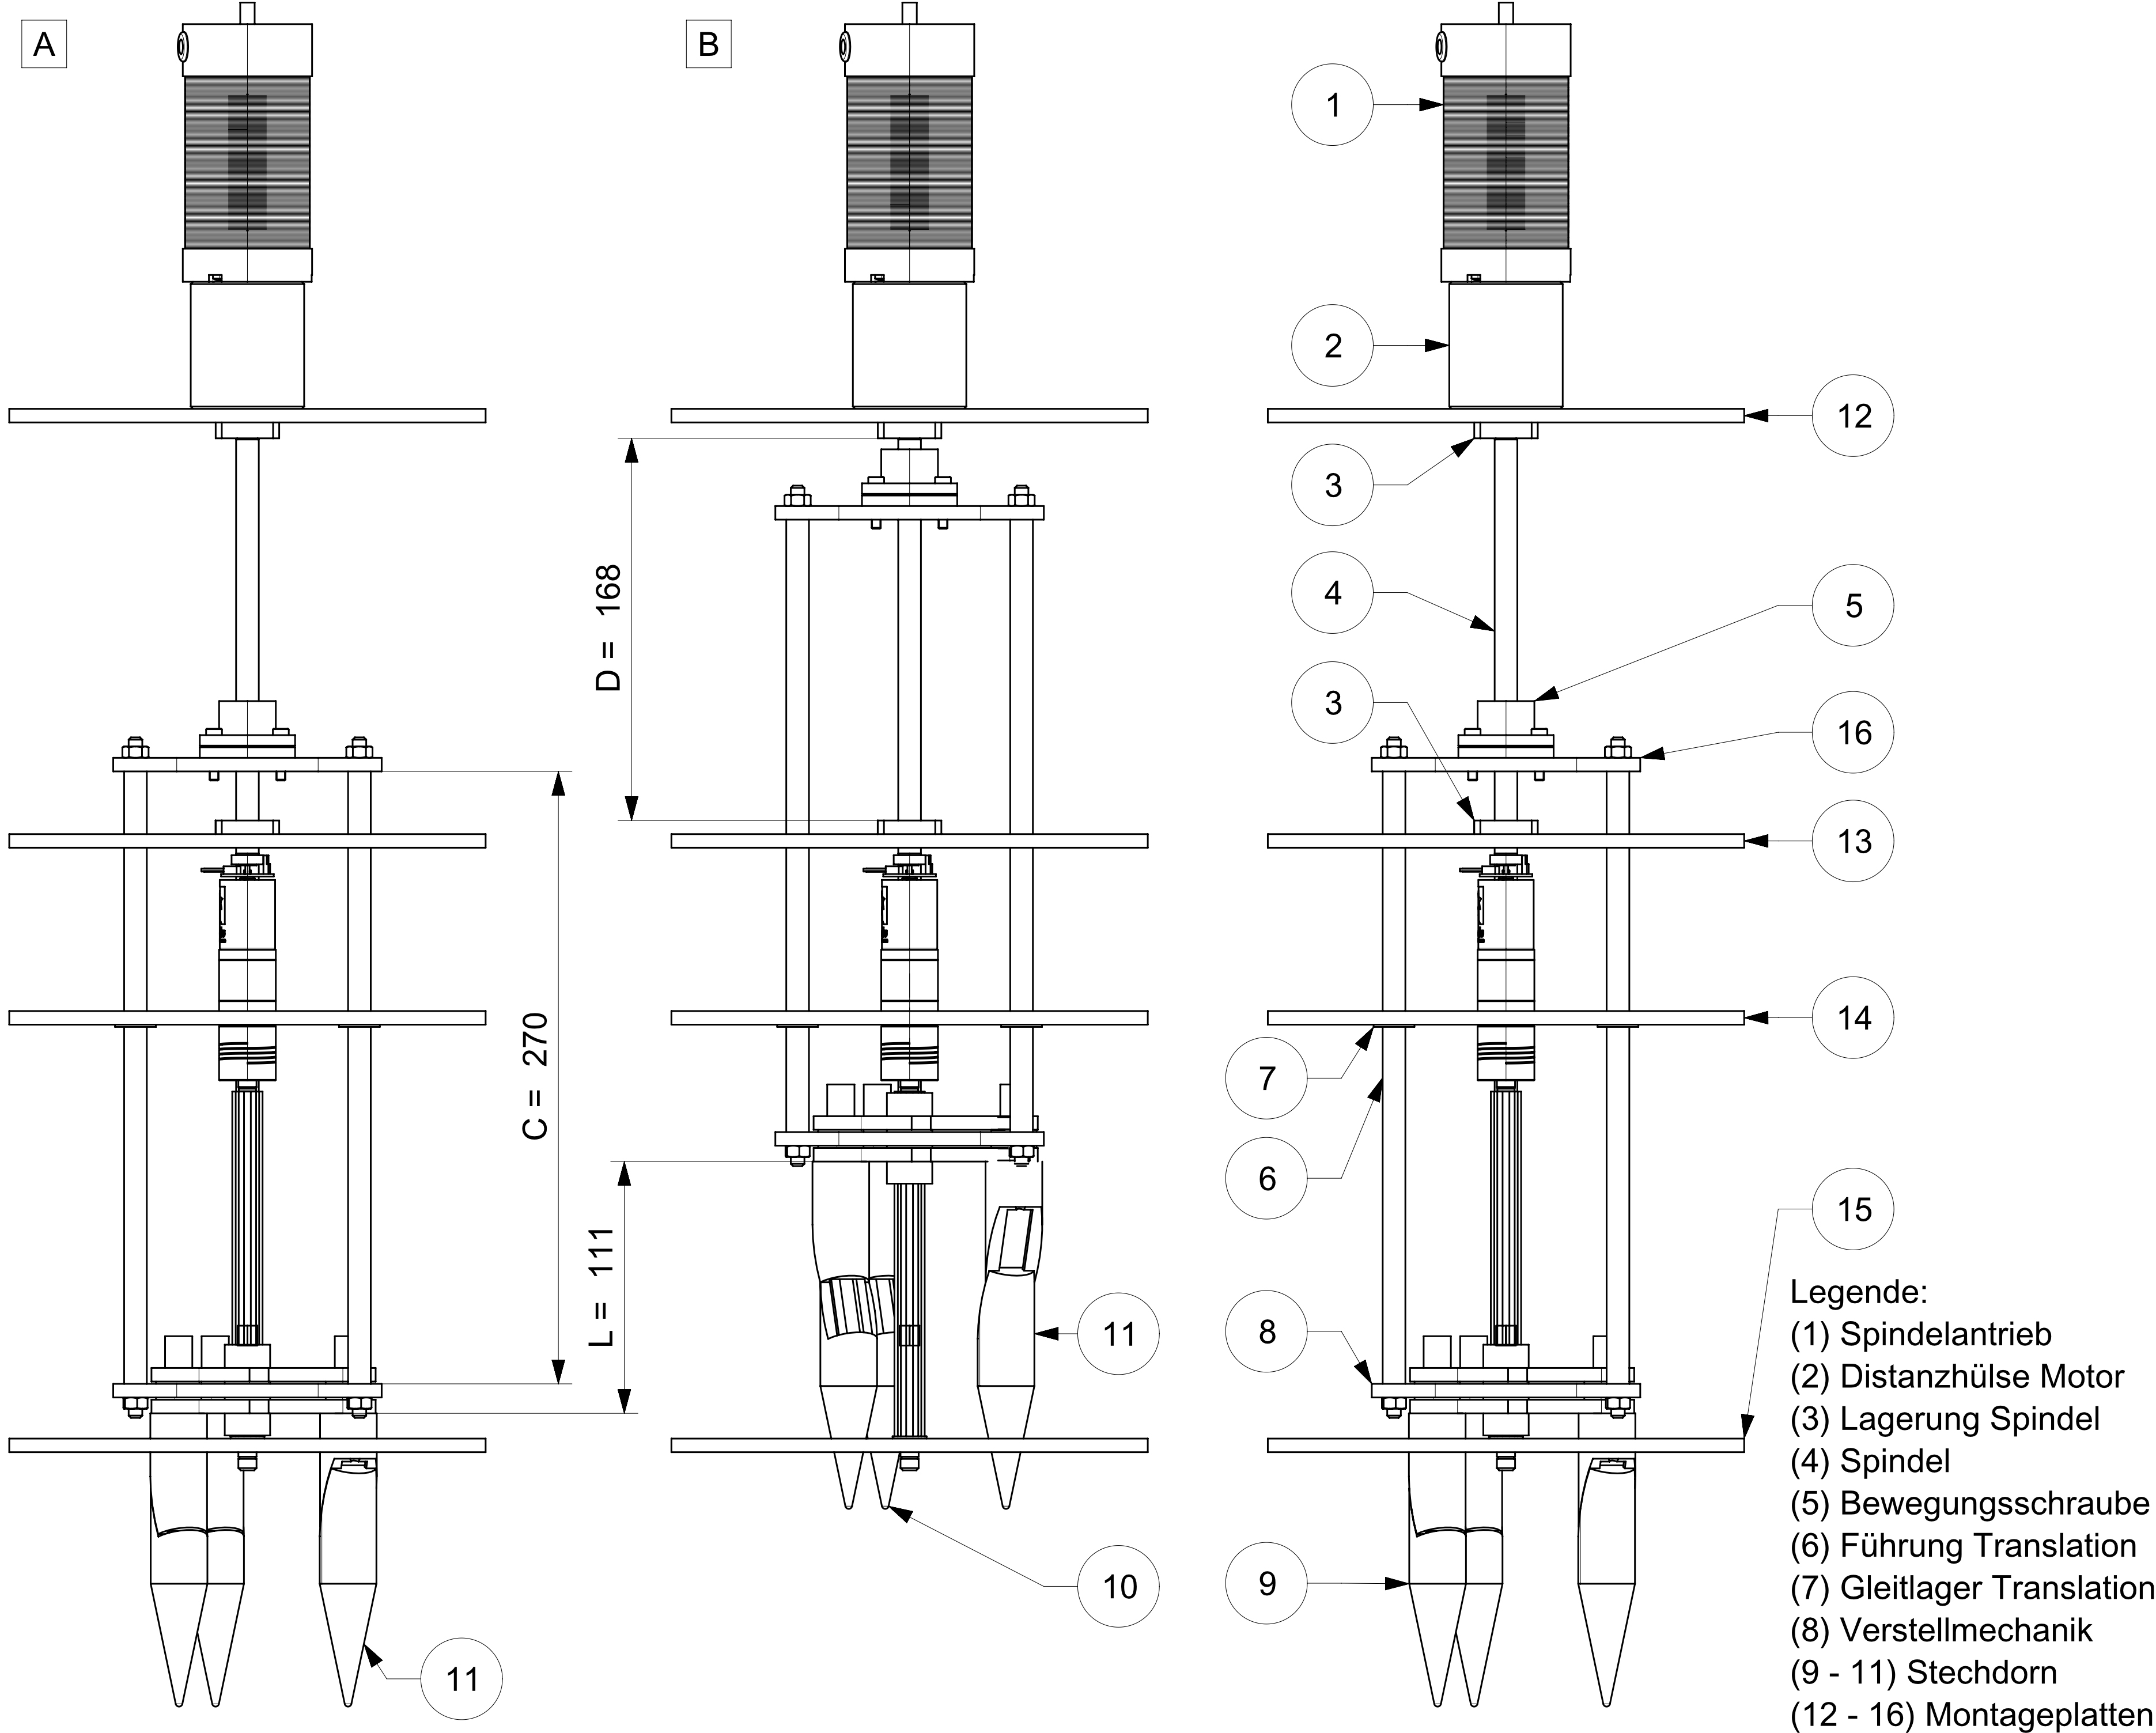
\includegraphics[scale=0.53]{Illustrationen/6-Umsetzung/setzeinheit_aio.jpg}
	\caption{Detaillierte Übersicht der Setzeinheit}
	\label{fig:setzeinheit}
\end{figure}

 
\subsubsection{Translation der Setzeinheit}
Um drei NemaCaps in einen Topf zu pflanzen, erfolgt folgender Prozess:
\begin{itemize}
	\item \textbf{A - Setzloch ausheben:} Die Spindel bewegt die Setzeinheit nach unten und treibt den Stechdorn in die Erde. Dadurch verschliesst sich der Stechdorn (Punkt 11 in Abb. \ref{fig:setzeinheit}). 

	\item \textbf{B - NemaCap setzen:} Nachdem die Erde verdrängt und das Setzloch ausgehoben ist, bewegt sich die Setzeinheit wieder nach oben. Nun öffnet sich der Stechdorn (10) indem sich der untere Teil durch die Schwerkraft seitlich nach unten bewegt. So können die NemaCaps in das ausgehobene Setzloch fallen.
\end{itemize}

Konstruktiv sind drei Masse hervorzuheben:
\begin{itemize}
	\item \textbf{L - Maximaler Hubweg:} Der maximale Hub L beträgt 111mm. Gemäss Berechnungen (Siehe Anhang: \textit{Auslegung Spindel}) muss dieser mindestens 86mm betragen. Somit beträgt die Reserve 25mm. 
	
	\item \textbf{C - Länge der Führungen:} Die Länge der Führungen ist gegeben durch den Hubweg L, der Höhe des Motors für die Verstellmechanik  und dessen Kupplung. Dies bedingt eine Länge von 270mm.
	
	\item \textbf{D - Länge der Spindel:} Die Spindellänge ergibt sich durch den maximalen Hub L und der Höhe der Bewegungsschraube (Punkt 5 in Abbildung \ref{fig:setzeinheit}) plus Montageplatte (15). Dadurch beträgt die Länge der Spindel 168mm.
\end{itemize}

\subsubsection{Spindel}
Die Wahl der Spindel und des Spindelantriebes haben einen entscheidenden Einfluss auf die Erfüllung des Setzprozesses innerhalb der vorgegeben Zeit. Parameter wie Steigung, Spindeldurchmesser und Material der Spindel wirken sich direkt auf die Massenträgheit und somit auf das erforderliche Beschleunigungsmoment aus.
\newline

Dieses Subkapitel befasst sich mit der Auslegung und Berechnung der Spindel. Dabei sind Berechnungen in zusammengefasster Form dargestellt. Der vollständige Rechenweg und die detaillierte Vorgehensweise sind im Anhang (Dokument \textit{Auslegung Spindel}) zu entnehmen.

Gegeben durch den Setzprozess und die Geometrie sind folgende Daten:
	\begin{figure}[H]
	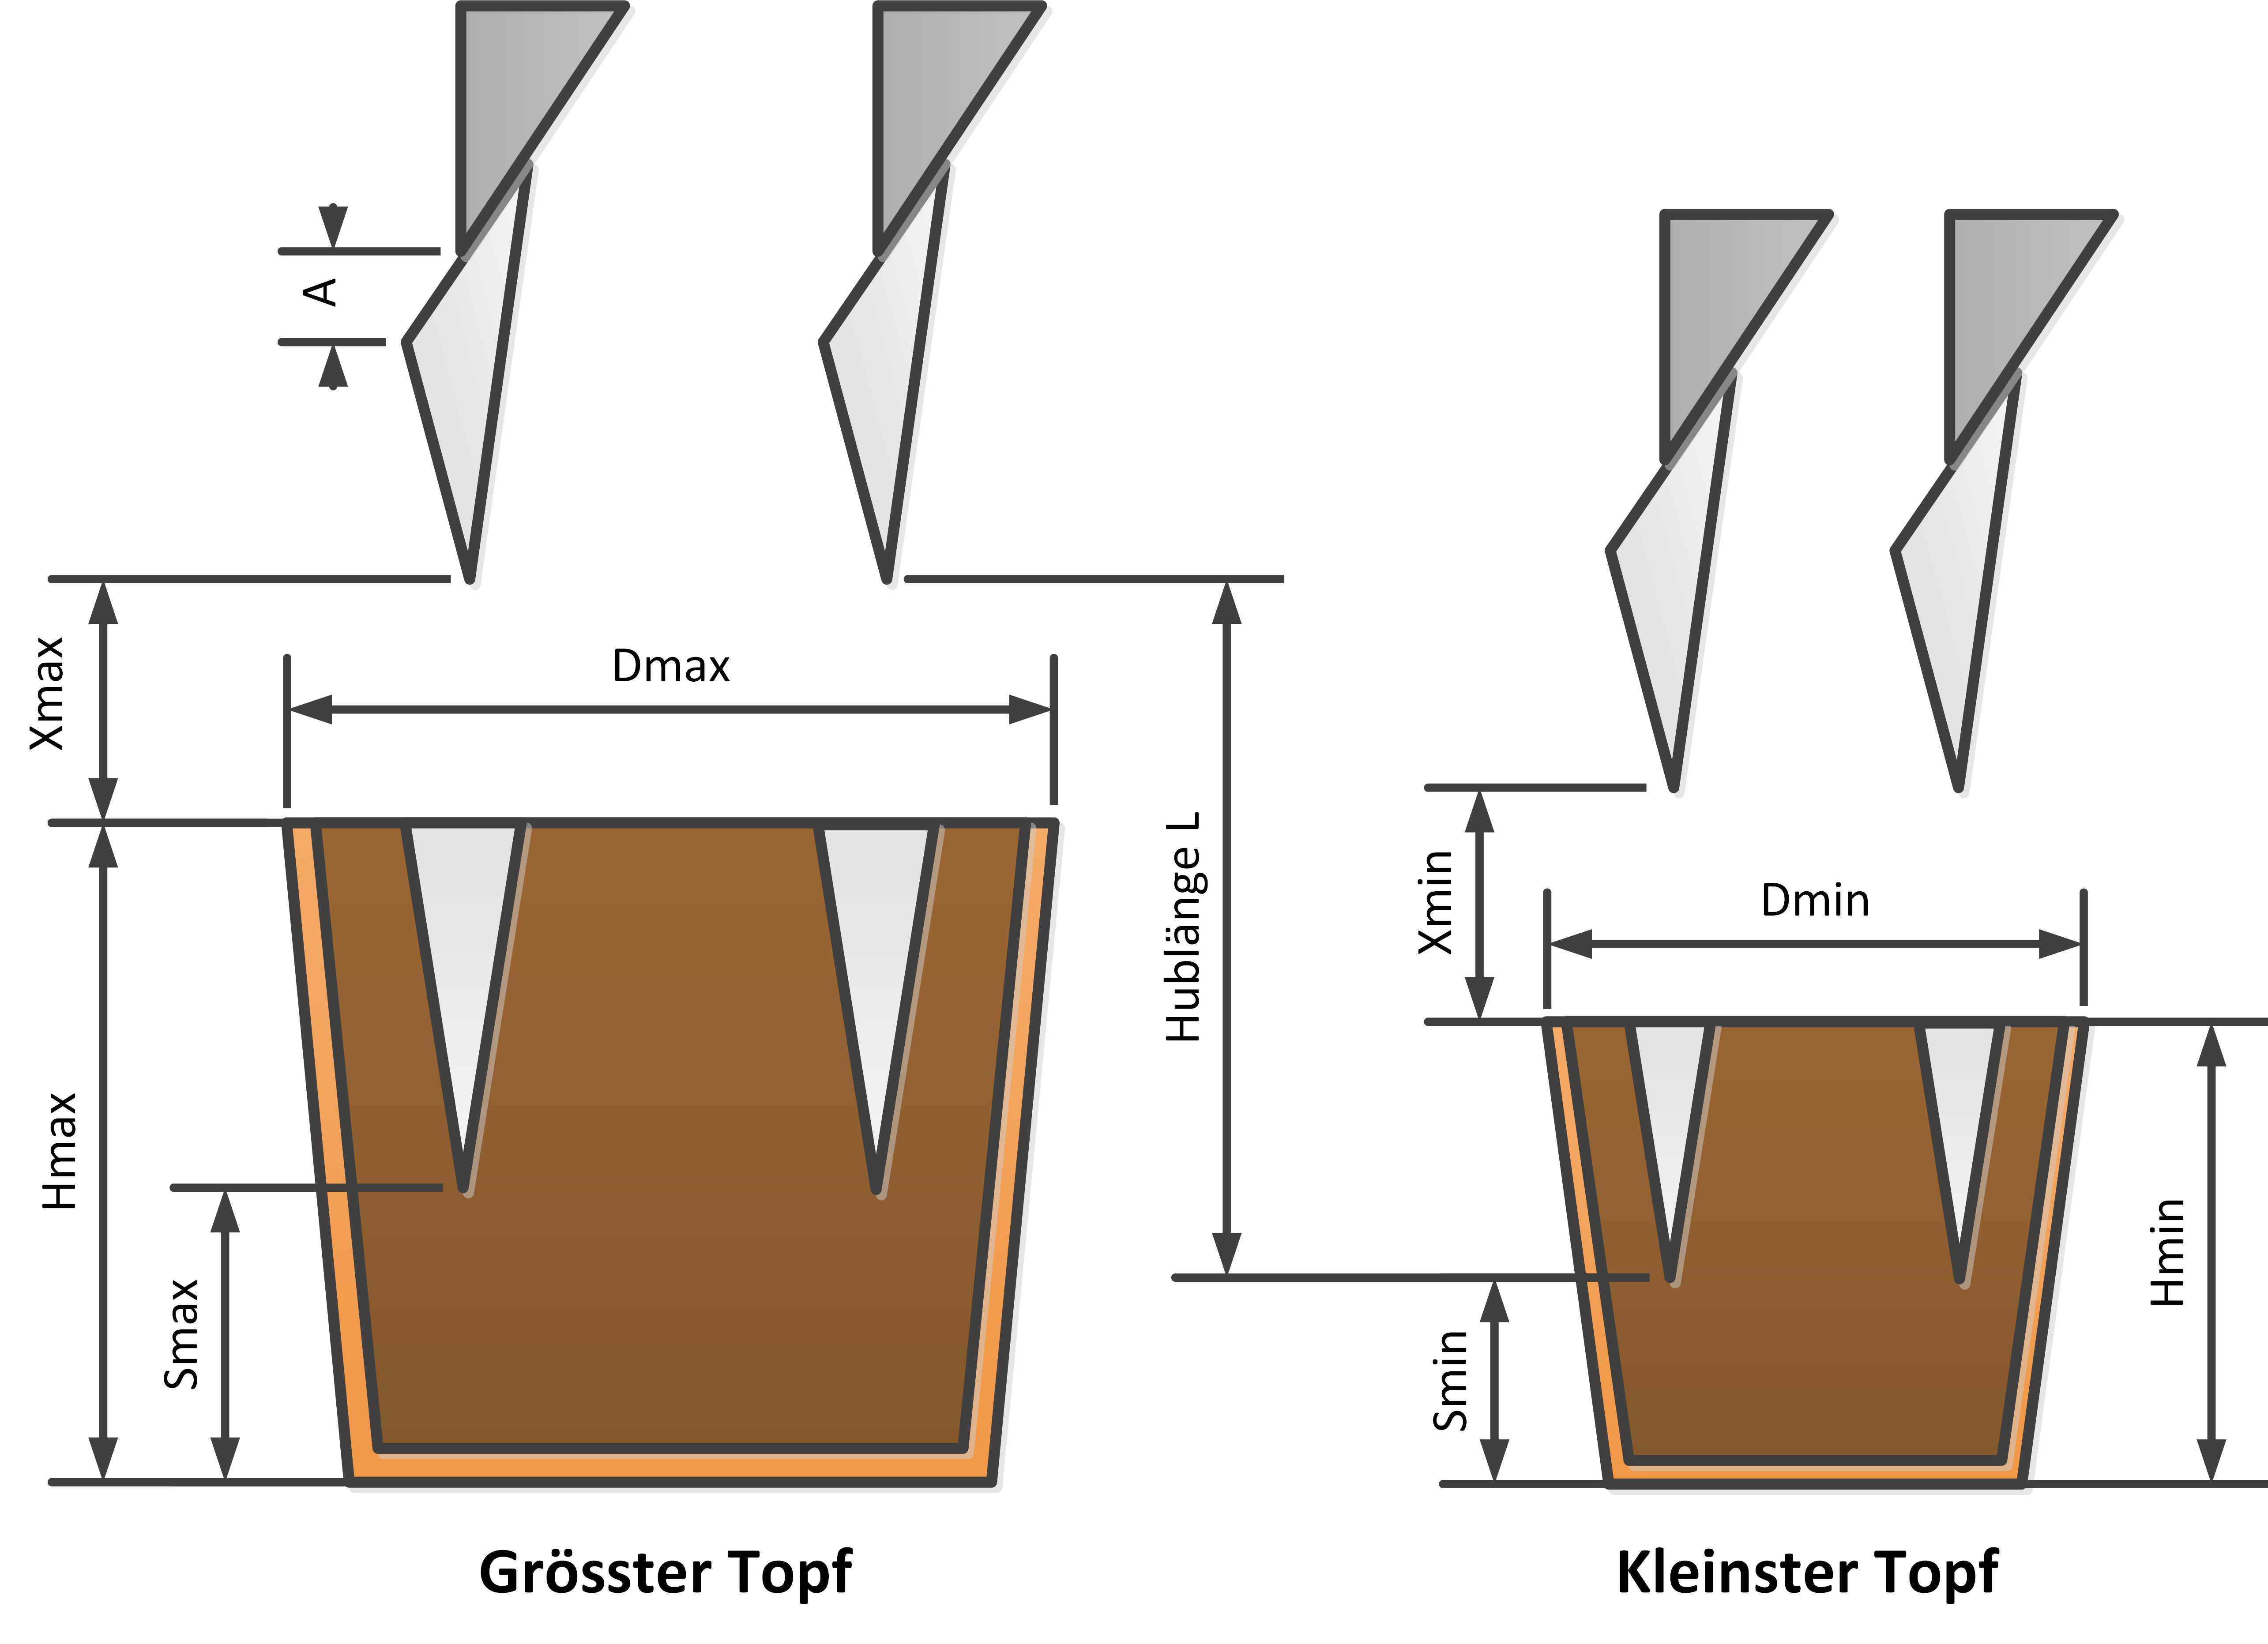
\includegraphics[width=1\textwidth]{Illustrationen/6-Umsetzung/topfgeometrie.png}
	\caption{Geometrie der Töpfe und des Setzprozess}
	\label{fig:topfgeometrie}
	\end{figure}
\begin{table}[H]
\begin{tabular}{|l|c|c|l|}
	\hline 
	& Grösster Topf (max) & Kleinster Topf (min) & Kommentar \\ 
	\hline 
	Durchmesser D [mm] & 140 & 90 & Aus Datenblatt \\ 
	\hline 
	Höhe h [mm] & 106 & 67 & Aus Datenblatt \\ 
	\hline 
	max. Einsetztiefe S [mm] & 63.6 & 40.2 & 0.6 x Höhe \\ 
	\hline 
	Sicherheitsabstand X [mm] & 15 & 15 & Annahme \\ 
	\hline 
	Ausfahrlänge A Dorn [mm] & 15 & 15 & Annahme \\ 
	\hline 
\end{tabular} 
	\caption{Randbedingungen für Spindelauslegung}
	\label{tab:Randbedingungen}
\end{table}

Anhand dieser Randbedingungen und den getroffenen Annahmen ergibt sich eine Beschleunigungs- und Bremszeit T\textsubscript{b}=0.1125s. Bei einem maximalen Hubweg U\textsubscript{max} = 72.4mm beträgt die grösste durschnittliche Geschwindigkeit v\textsubscript{avmax}:

\begin{equation}
v_{avmax}=\frac{U_{max}}{t_{b}}=\frac{72.4mm}{0.1125s}=643.5mm/s
\end{equation}
\newline
Die Geschwindigkeit des Dornes kann  gemäss Abbildung \ref{fig:vprofil_dorn} streng idealisiert dargestellt werden:
	\begin{figure}[H]
	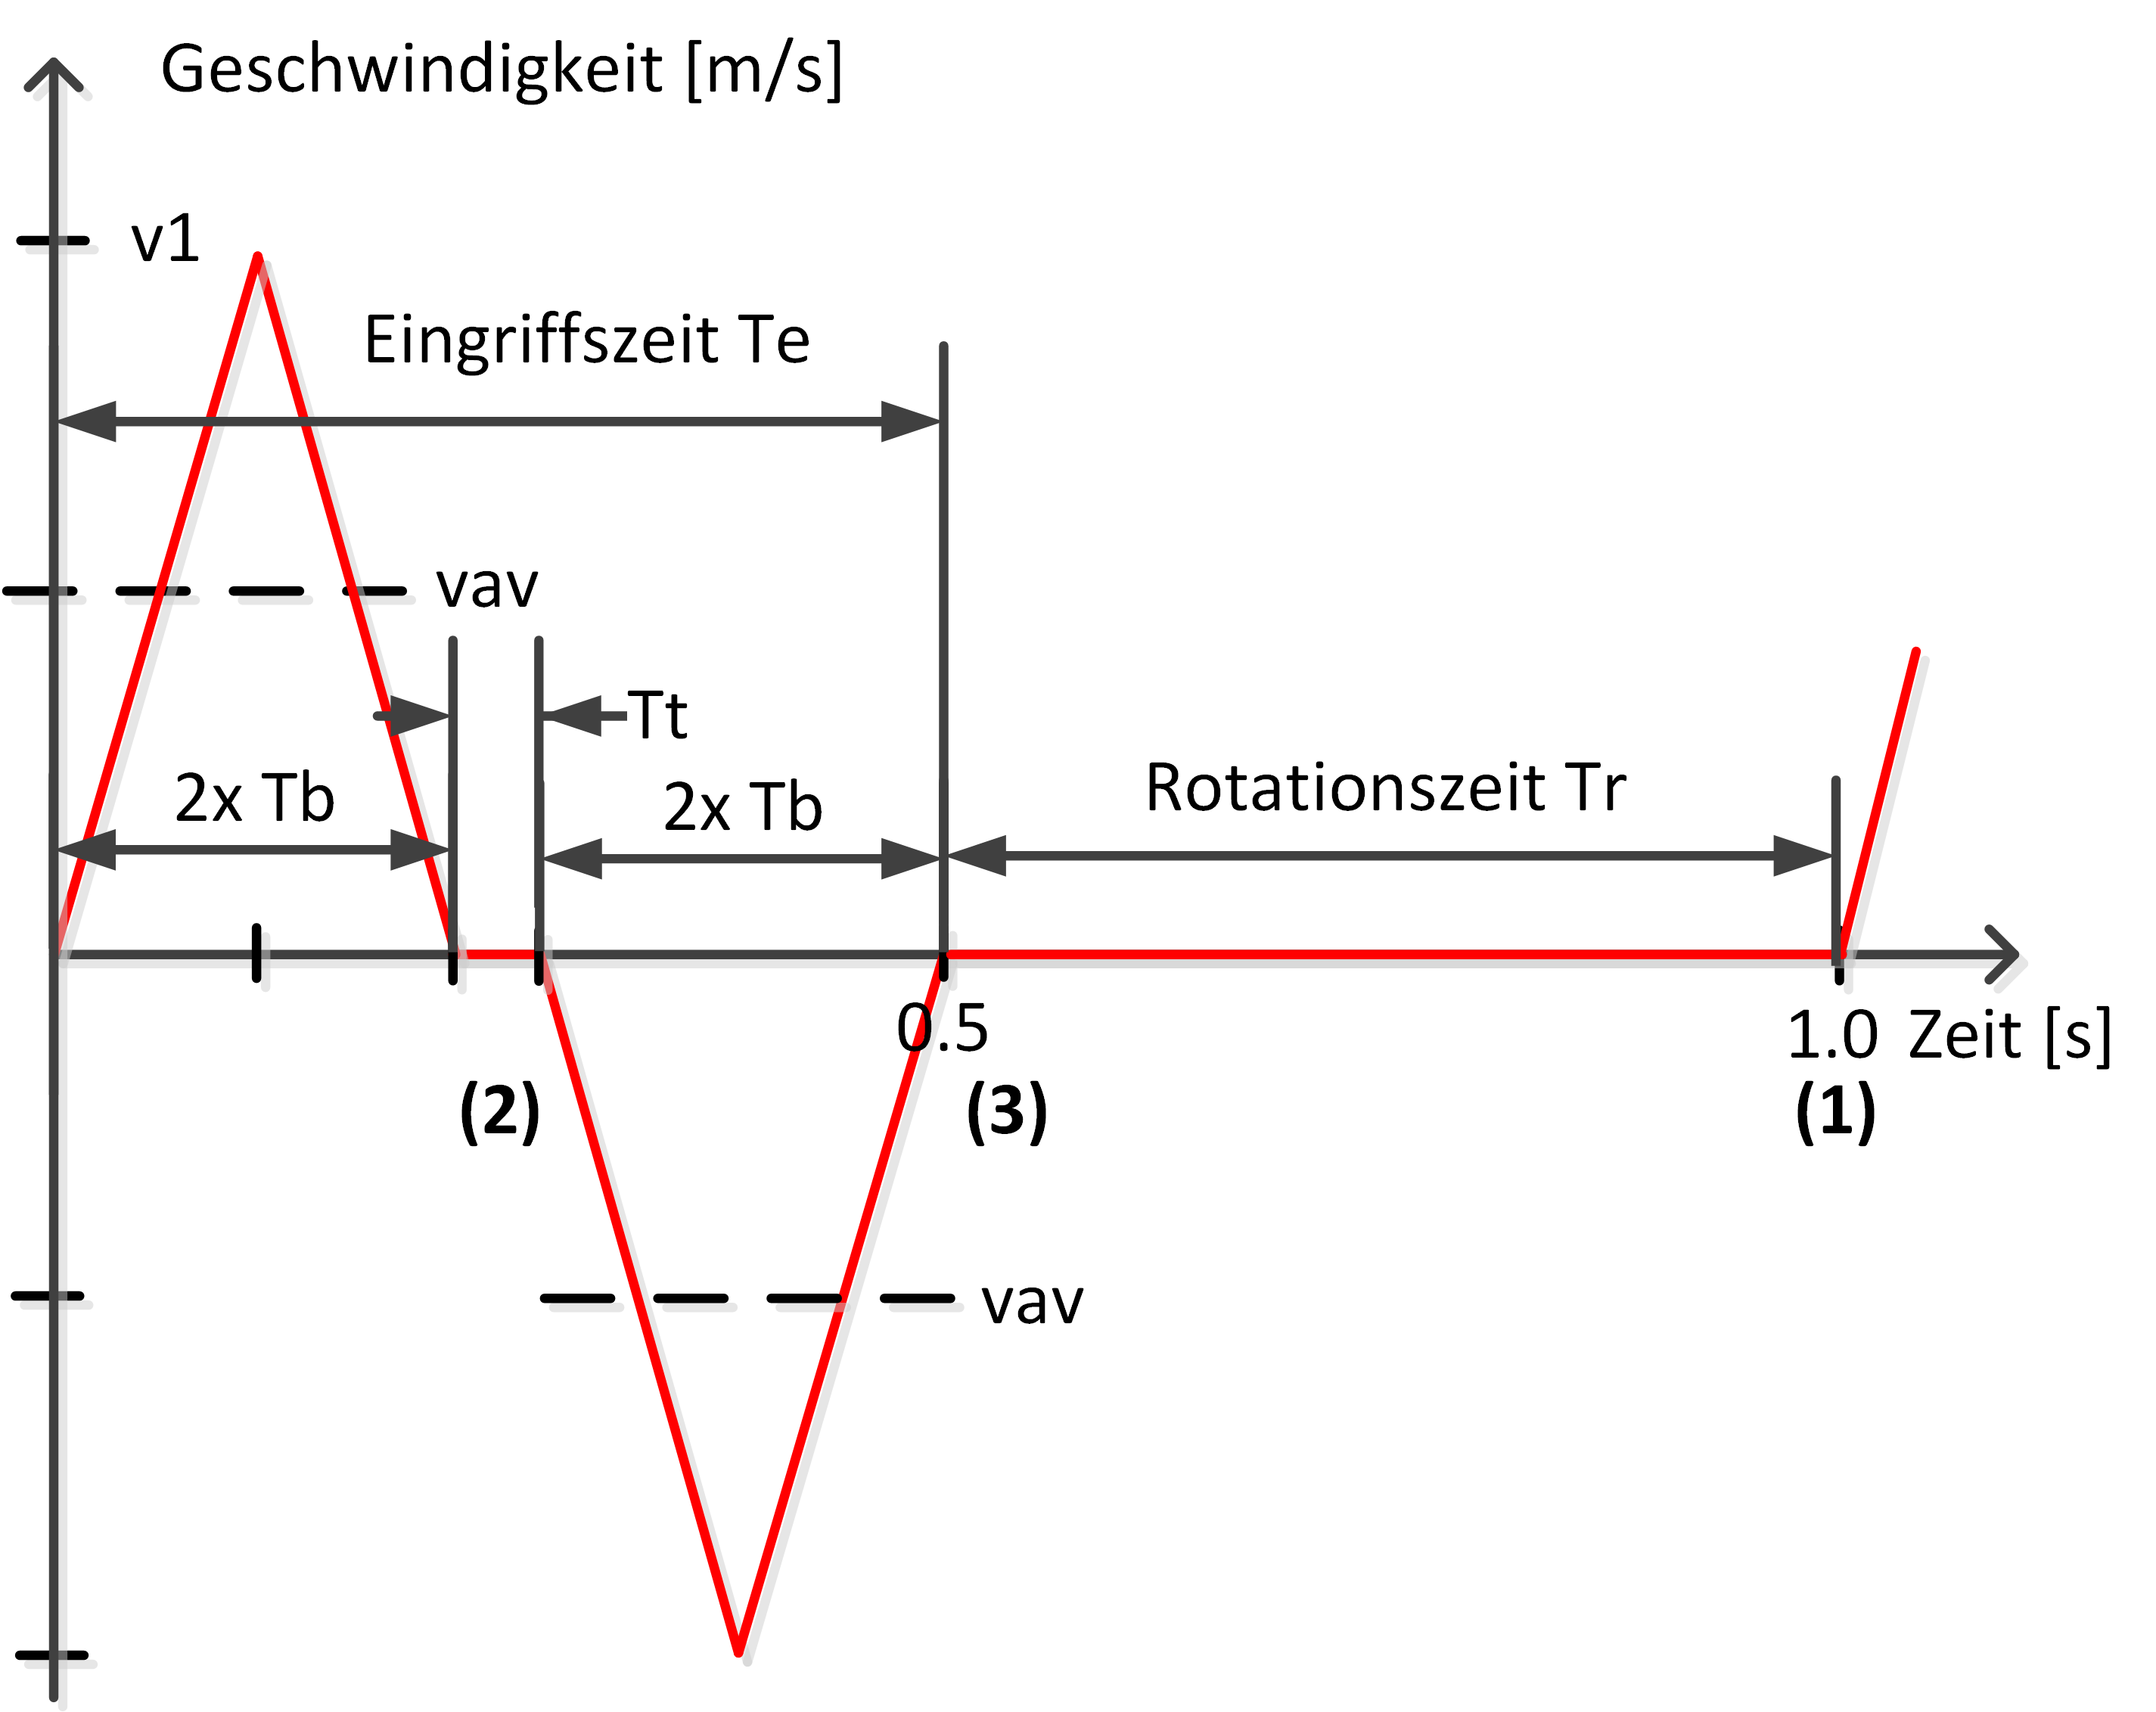
\includegraphics[width=1\textwidth]{Illustrationen/6-Umsetzung/vprofil_dorn.png}
	\caption{Geschwindigkeitsprofil des Dorns}
	\label{fig:vprofil_dorn}
\end{figure}
Orientiert an den Anforderungen aus Kapitel \ref{subsec:Translation} und der berechneten Geschwindigkeit sind vier Steilgewindespindeln von Igus ausgewählt worden. In Rücksprache mit Mark Chalençon, Produktmanager bei igus Schweiz GmbH, wurde die Auswahl der Produkte zusätzlich verifiziert (E-Mail vom 18.4.17).
\begin{table}[H]
\begin{tabular}{|c|c|}
	\hline 
	Ds14x30 (Edelstahl) & Ds10x25 (Edelstahl) \\ 
	\hline 
	Ds14x30 (Aluminium) & Ds10x25 (Aluminium) \\ 
	\hline 
\end{tabular} 
\caption{Ausgewählte Steilgewindespindeln von Igus}
\label{tab:spindeln}
\end{table}
Mit diesen Angaben kann die Spindel durch ein reduziertes Model dargestellt werden, analog zu Abbildung 13-5, S.448 \cite{roloffmatek}:
 	\begin{figure}[H]
 	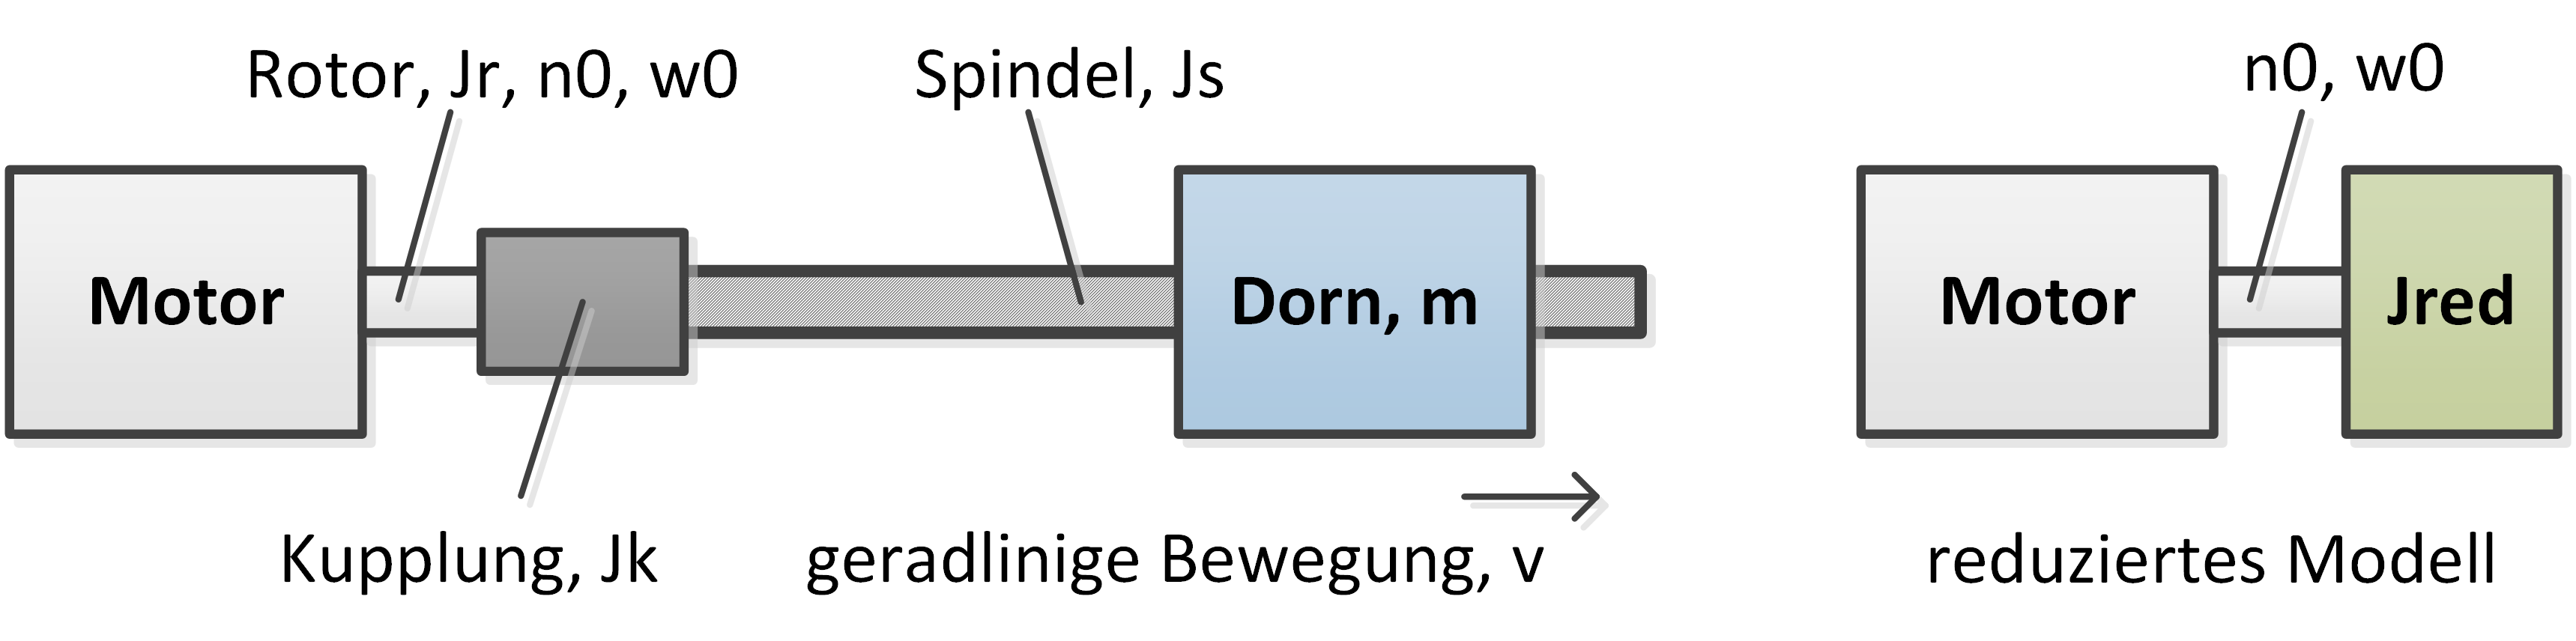
\includegraphics[width=1\textwidth]{Illustrationen/6-Umsetzung/red_modell.png}
 	\caption{Schema des Spindelantriebs sowie des reduzierten Modells}
 	\label{fig:red_modell}
	\end{figure}
Wobei für das reduzierte Modell sich die reduzierte Massenträgheit J\textsubscript{red} und das benötigte Beschleunigungsmoment M\textsubscript{a} ergibt (Gleichung 13.3 und 13.4, S.449):
\begin{equation}
J_{red}=J_{rotor}+J_{kupplung}+J_{spindel}+m*(\frac{v_{1}}{w_{v1}})^{2}
\end{equation}
\begin{equation}
M_{a}=J_{red}*\frac{w_{2}-w_{1}}{t_{b}}=J_{red}*\frac{w_{v1}}{t_{b}}
\end{equation}
Für die ausgewählten Spindeltypen ergibt dies folgende Werte:

\begin{table}[H]
\begin{tabular}{|c|c|c|}
	\hline 
	& reduzierte Massenträgheit J\textsubscript{red}& Beschleunigungsdrehmoment M\textsubscript{a}\\ 
	\hline 
	Ds14x30 Edelstahl & 5.36E-05 & 0.128 \\ 
	\hline 
	Ds14x30 Aluminium & 4.93E-05 & 0.118 \\ 
	\hline 
	Ds10x25 Edelstahl & 4.16E-05 & 0.120 \\ 
	\hline 
	Ds10x25 Aluminium & 4.05E-05 & 0.116 \\ 
	\hline 
	Einheit & kgm$^2$ & Nm \\ 
	\hline 
\end{tabular} 
\caption{Reduzierte Massenträgheit J\textsubscript{red} und benötigtes Beschleunigungsdrehmoment M\textsubscript{a} der ausgewählten Spindeln}
\label{tab:spindel_final}
\end{table}
Die berechneten Werte für das Beschleunigungsmoment M\textsubscript{a} aus Tabelle \ref{tab:spindel_final} zeigen, dass sich alle ausgewählten Spindeln für den evaluierten Spindelantrieb eignen.
\newline
Als definitive Wahl wird die Spindel \textbf{Ds10x25 aus Edelstahl} ausgewählt. Folgende Argumente sind ausschlaggebend:
	\begin{itemize}
	\item Die Variante Ds10x25 aus Edelstahl bietet das Optimum von geringem Durchmesser und hoher Festigkeit. Das leicht höhere Beschleunigungsmoment der Ds10x25 aus Edelstahl zur Ds14x30 wird für eine höhere Festigkeit in Kauf genommen.
	
	\item \ Die geringere Steigung gibt dem Motor mehr Weg (Umdrehungen) zur Beschleunigung.
\end{itemize}
Die Ausgewählte Spindel verfügt somit über eine Reserve S von 3.5 gegenüber dem verfügbaren Beschleunigungsdrehmoment des Antriebs (Siehe Anhang: \textit{Auslegung Spindel}).

\subsubsection{Kupplung}
Zur mechanischen Verbindung zwischen Spindelantrieb und Spindel wird eine drehstarre Kupplung verwendet. Dadurch kann eine winkelgetreue Drehmomentenübertragung gewährleistet werden, was für diese Anwendung essentiell ist \cite{dubbel}. Hierfür wird die Kupplung HELICAL WA 20-8-6 aus Aluminium von Ringspann AG verwendet \cite{helical}. Die Wahl eines kleinen Aussendurchmessers (20mm) und ein leichter Werkstoff sind für ein möglichst geringes zusätzliches Trägheitsmoment entscheidend und wurde hier berücksichtigt.

\subsubsection{Lagerung}
\textbf{Rotation der Spindel}
\newline
Die Spindel wird durch ein Fest- sowie ein Loslager eindeutig gelagert. Das Festlager ist in der obersten Montageplatte (Punkt. 12 in Abb. \ref{fig:setzeinheit}) vorgesehen, das Loslager hingegen in der zweiten Montageplatte (13). Diese Anordnung ist bewusst so gewählt, damit das Festlager Axialkräfte aufnimmt und der Spindelantrieb axial unbelastet bleibt. Für die Lagerung werden fertige Lagerböcke von Mädler Norm-Antrieb AG verwendet, welche speziell für Spindeln ausgelegt sind. Diese sind einfach im Einbau und erfordern keinen zusätzlichen Entwicklungsaufwand. An der Spindel wird konstruktiv einen Freistich Form E umgesetzt (Siehe Anhang: \textit{Spindel DST LS 10x25})\cite{vsm}.
\newline

\textbf{Translation der Setzeinheit}
\newline
Die Lagerung der translatorischen Bewegung wird durch drei Gleitlager (Punkt. 7 in Abb. \ref{fig:setzeinheit}) realisiert. Dabei werden diese in die Montageplatte (14) eingepresst. Dafür werden drei Kunststoff Gleitlager iglidur JSM-1012 von igus verwendet. Begründet wird die Wahl dadurch, dass Kunstoffgleitlager schmiermittel- und wartungsfrei sind, geringe Reibwerte und eine hohe Lebensdauer aufweisen. Weiter sind dies Standard-Maschinenelemente und dadurch günstig erhätlich. Weitere Informationen die Gleitlager sind aus dem Datenblatt zu entnehmen \cite{igusJSM}.


\subsubsection{Montage}
Wie schon mehrfach erläutert werden verschiedenste Komponenten an Montageplatten montiert. Wie aus Abbildung \ref{fig:setzeinheit} ersichtlich, werden die Montageplatten vertikal angeordnet. Diese Anordnung bildet das Gerüst für eine funktionierende Setzeinheit. Wie in Kapitel \ref{sec:Vereinzelung} erwähnt, bietet sich die konsequente Fertigung mittels Lasermaschine an. Mechanisch fixiert werden die Montageplatten durch Aluminium Profile der Firma Kanya AG (weitere Informationen: siehe Kapitel \ref{maschinengestell}), wobei durch die Nut der Profile eine Blechdicke von 6mm vorgegeben ist. Diese Konstruktion bringt folgende Vorteile:
	\begin{itemize}
	\item Komponenten können auf unterschiedlichen Ebenen angeordnet werden. Weiter ist das Hinzufügen von weiteren Komponenten auf einfachste Art realisierbar. Wird eine weitere Komponente benötigt, wird die entsprechende Kontur (z.B. ein Langloch oder Bohrung) vorgesehen und die Komponente kann montiert werden.
	\item Die Fixierung der Montageplatten durch Aluminium-Profile bringt weitere Flexibilität bei der Montage. Dadurch bleibt die Höhe der einzelnen Platten verstellbar. Auch seitlich können die Platten in eine Richtung verstellt werden.
\end{itemize}
 	\begin{figure}[H]
	\includegraphics[width=1\textwidth]{Illustrationen/6-Umsetzung/Montageplatten.png}
	\caption{Übersicht der Montageplatten}
	\label{fig:montageplatten}
\end{figure}
Die Montageplatten 1 bis 3 aus Abbildung \ref{fig:montageplatten} verfügen über drei Langlöcher (Detail A), welche um jeweils 120° verschoben angeordnet sind. Diese sind für die flexible Führung der Schläuche vorgesehen.
\subsection{Verstellmechanik}
\label{verstellmechanik}
\textit{(ygu)} Die Hauptaufgabe der Verstellmechanik ist die automatisierte Einstellung aller geforderten Topfradien. Die Verstellmechanik bildet einen Teil der Setzeinheit. Dabei kann keine klare Abgrenzung zur Setzeinheit gemacht werden, da in gewissen Komponenten Funktionen beider Einheiten vereint sind. Auch ist die Verstellmechanik klar als Wunschanforderung formuliert. Die Wunschanforderung birgt einen erhöhten Entwicklungsaufwand. Dieser Mehraufwand wird bewusst eingegangen, um ein Maximum an Automatisierungsgrad zu erreichen. Sollte trotzdem auf die automatische Verstellung der Topfradien verzichtet werden, ist die Entwicklung der Pflichtanforderung weniger zeitintensiv und rasch implementiert.
\subsubsection{Aufbau}
Die Konstruktion der Verstellmechanik basiert auf dem erstellten Funktionsmuster. Die Grundidee ist, dass über zwei Kulissen (eine radiale und eine lineare) der Topfradius zentral an einer Welle verstellt werden kann. Ein klarer Vorteil ist, dass dadurch nur ein Aktor für die Verstellung aller Stechdorne benötigt wird. Die Konstruktion kann in zwei Teile unterteilt werden:
\begin{itemize}
	\item \textbf{dynamischer Teil}: Dieser Teil wird durch die Spindel bewegt. Die drei Stechdorne (Punkt 4 in Abb. \ref{fig:details_vm}) sind durch zwei Kulissen (2, 3) verstellbar gelagert. Durch die Verbindung Keilnabe (5) - Keilwelle (1) sind diese mit dem statischen Teil gekoppelt. Eine geringes Gewicht des bewegten Teils ist für die Beschleunigung dieser Masse essentiell.
	
	\item \textbf{statischer Teil:} Der statische Teil dieser Einheit führt die Verstellung der Topfradien aus. Ein Getriebemotor (8), welcher durch eine Kupplung (9) mit der Keilwelle verbunden ist, führt die Verstellung der Topfradien aus. Diese Umsetzung besticht dadurch, dass anhand der Verbindung Keilnabe (5) - Keilwelle (1) bedeutend weniger Masse translatorisch beschleunigt wird. Dies bringt wertvolle Gewichteinsparnisse und wirkt sich positiv auf das benötigte Beschleunigungsdrehmoment M\textsubscript{a} aus.
\end{itemize}
	\begin{figure}[H]
	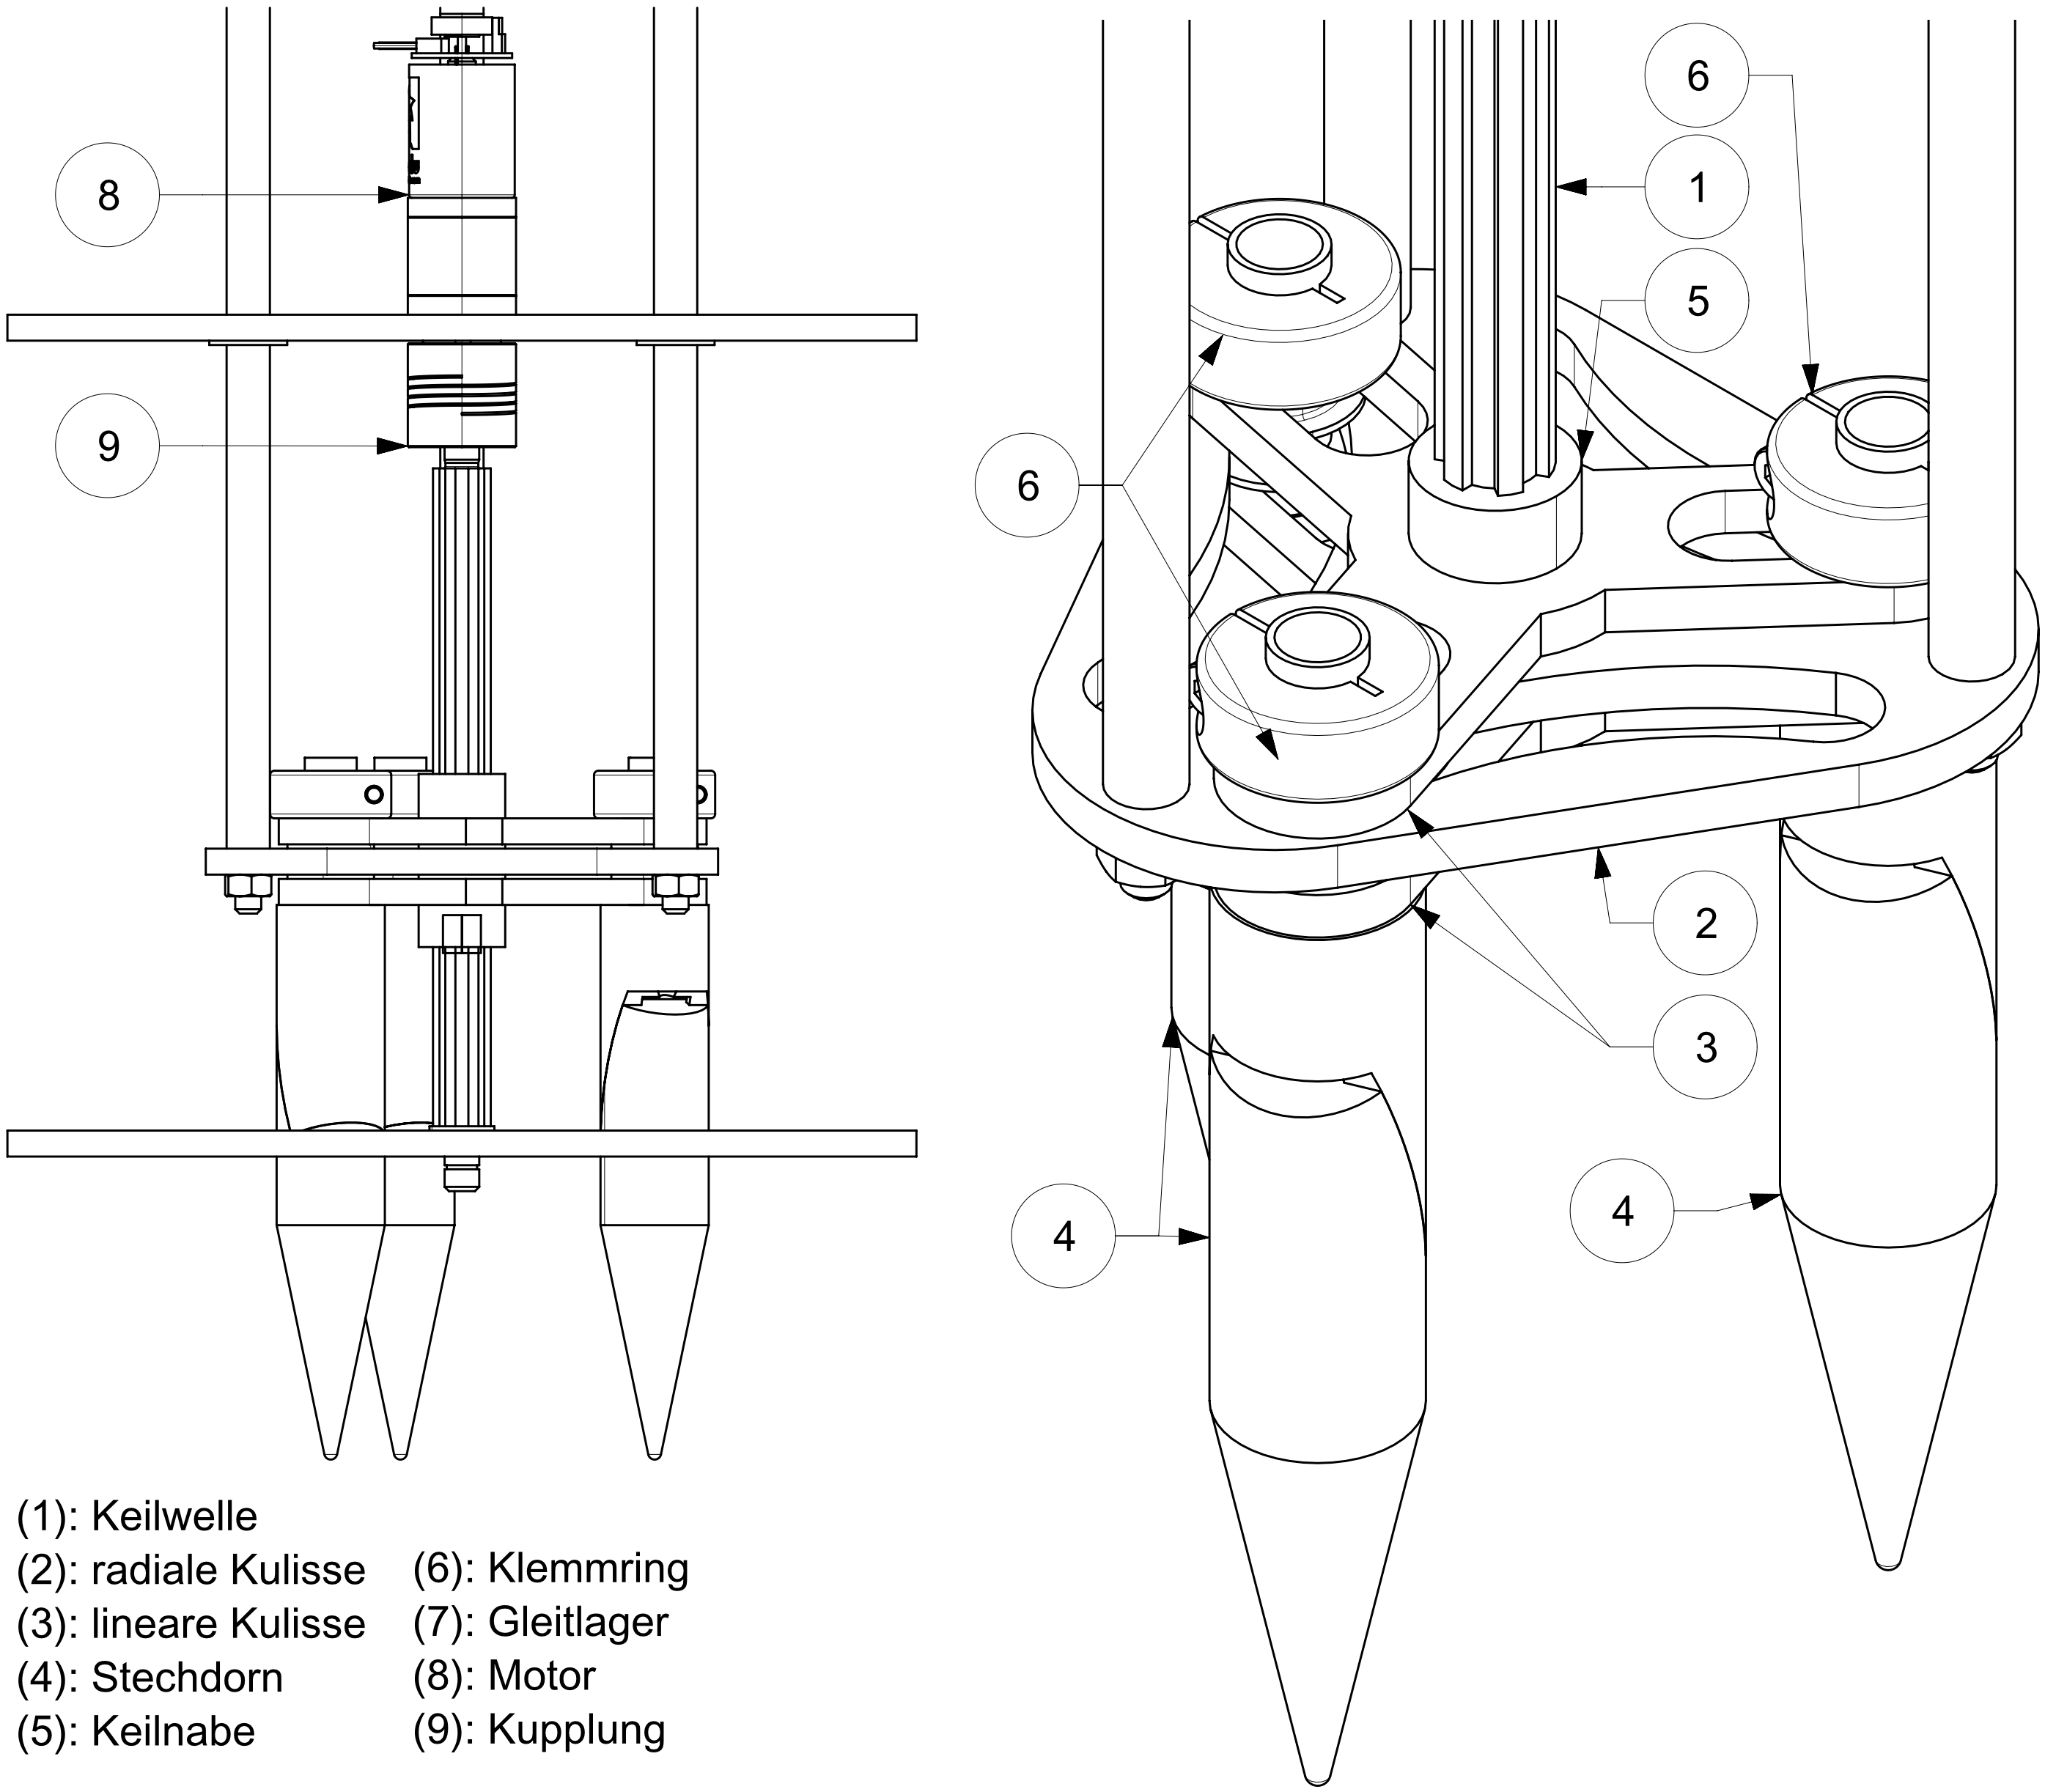
\includegraphics[scale=0.6]{Illustrationen/6-Umsetzung/details_vm.jpg}
	\caption{Detaillierte Übersicht der Verstellmechanik}
	\label{fig:details_vm}
	\end{figure}
Die Lagerung der Keilwelle wird nur wenig beansprucht, da durch die translatorische Freiheit der Keilnabe (entlang der Achse) keine Axialkräfte auftretten. Da die Verstellung des Topfradius nur wenige Male pro Tag vorgenommen wird, kann gemäss Roloff Matekk (Kapitel 14.3.1) von einer statischen Belastung (da n<10U/min) ausgegangen werden \cite{roloffmatek}. Daher ist die Verwendung eines Gleitlagers am unteren Ende (10) ausreichend. Verwendet wird das Gleitlager idlidur J3FM-0810 von Igus \cite{igusJ3FM}. Am oberen Ende ist die Keilwelle (1) über die Kupplung (9) durch den Getriebemotor (8) gelagert.
\newline

Der Stechdorn wird durch zwei lineare Kulissen (Punkt 3 in Abb \ref{fig:schnitt_vm}) und eine radiale Kulisse (2) geführt. Dabei sind die linearen Kulissen (3) mit der Keilnabe verbunden, die Radiale über die Führungen mit der Spindel. Um die Reibung zwischen Stechdorn und Kulissen zu vermindern werden auch hier Gleitlager (7) von igus eingesetzt. Die ganze Mechanik wird dabei durch die Auflage des Stechdorns (4) und einem Klemmring (6) gehalten.
	\begin{figure}[H]
	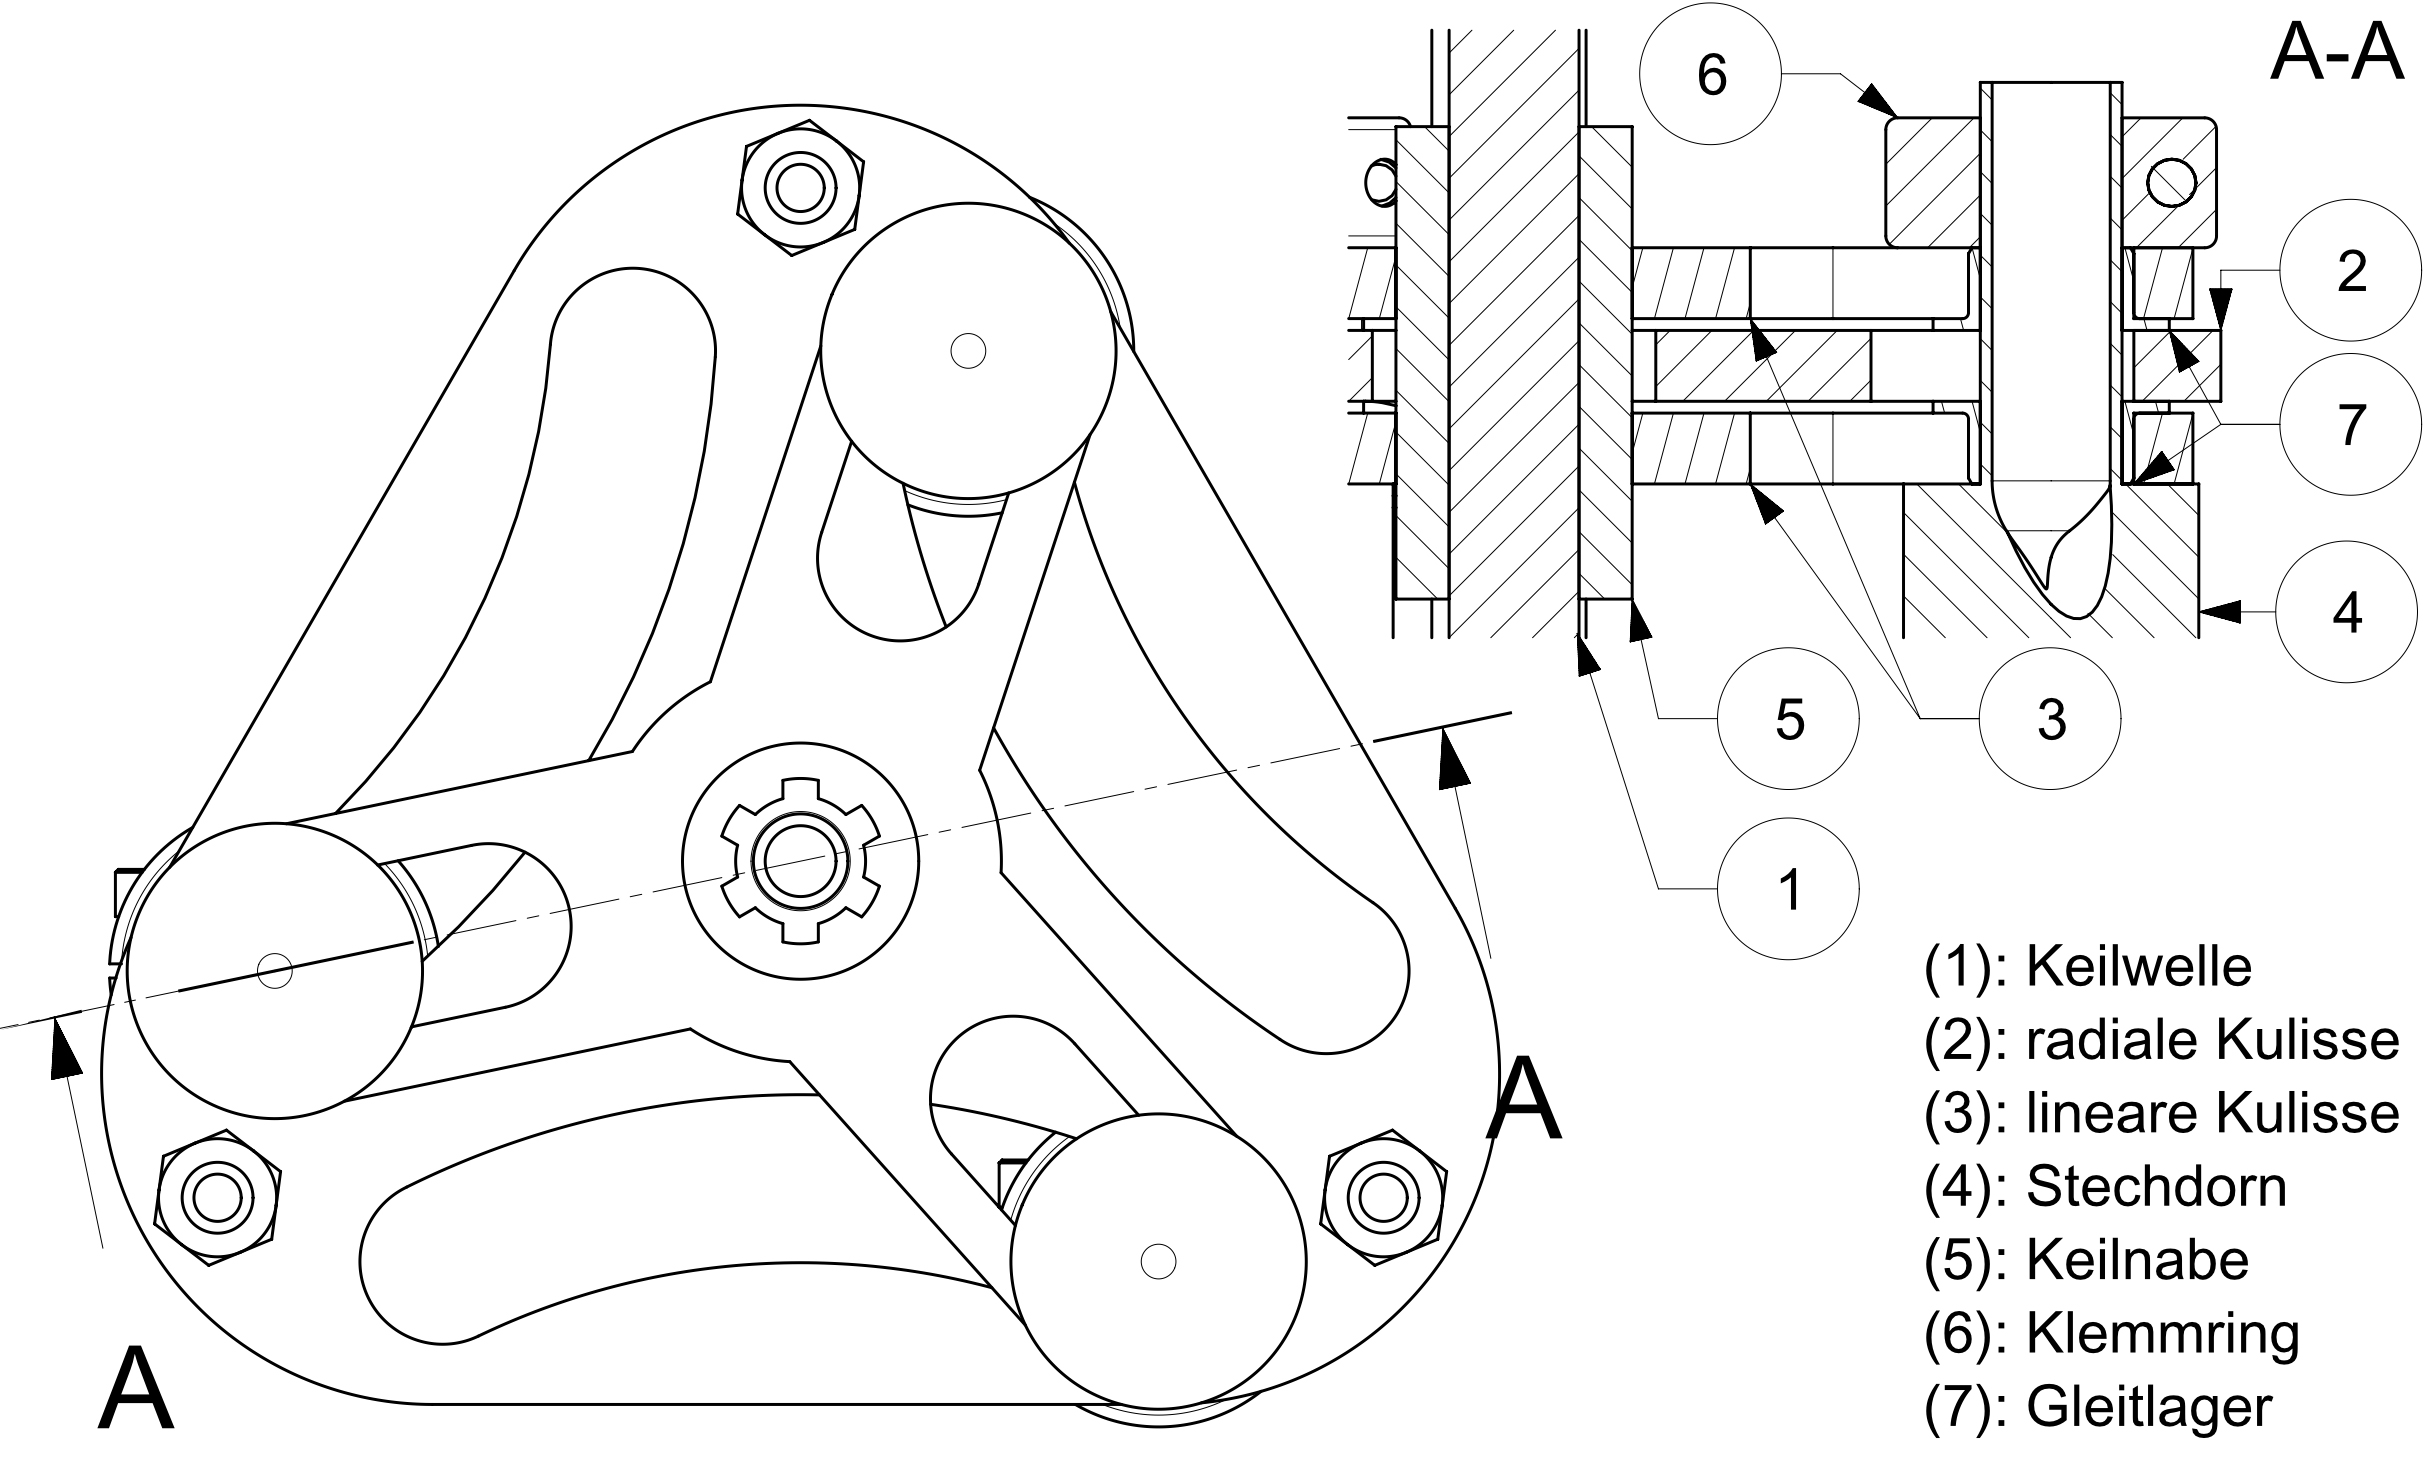
\includegraphics[scale=0.63]{Illustrationen/6-Umsetzung/schnitt_vm.jpg}
	\caption{Geschnittene Seitenansicht der Verstellmechanik}
	\label{fig:schnitt_vm}
	\end{figure}

\subsubsection{Funktion}
Die Bewegung der Verstellmechanik ist in Abbildung \ref{fig:motion_vm} dargestellt. Punkt B bildet ein beliebiger Punkt ab. Damit wird am Anschlag (Punkt A aus Abb. \ref{fig:motion_vm}) die Einsetzlokalität des grössten Topfes (Dmax = 140mm) und bei halbem Weg der Kulisse die Einsetzlokalität des kleinsten Topfes (Dmin = 90mm) erreicht. Dabei fällt auf, dass das Doppelte des nötigen Weges implementiert wurde. Begründet wird dies damit, dass dadurch der hochübersetzte Getriebemotor mehr Umdrehungen absolviert, bis der gewünschte Radius erreicht wird. Dies steigert die Auflösung des Motors und verbessert die Regelbarkeit.
	\begin{figure}[H]
	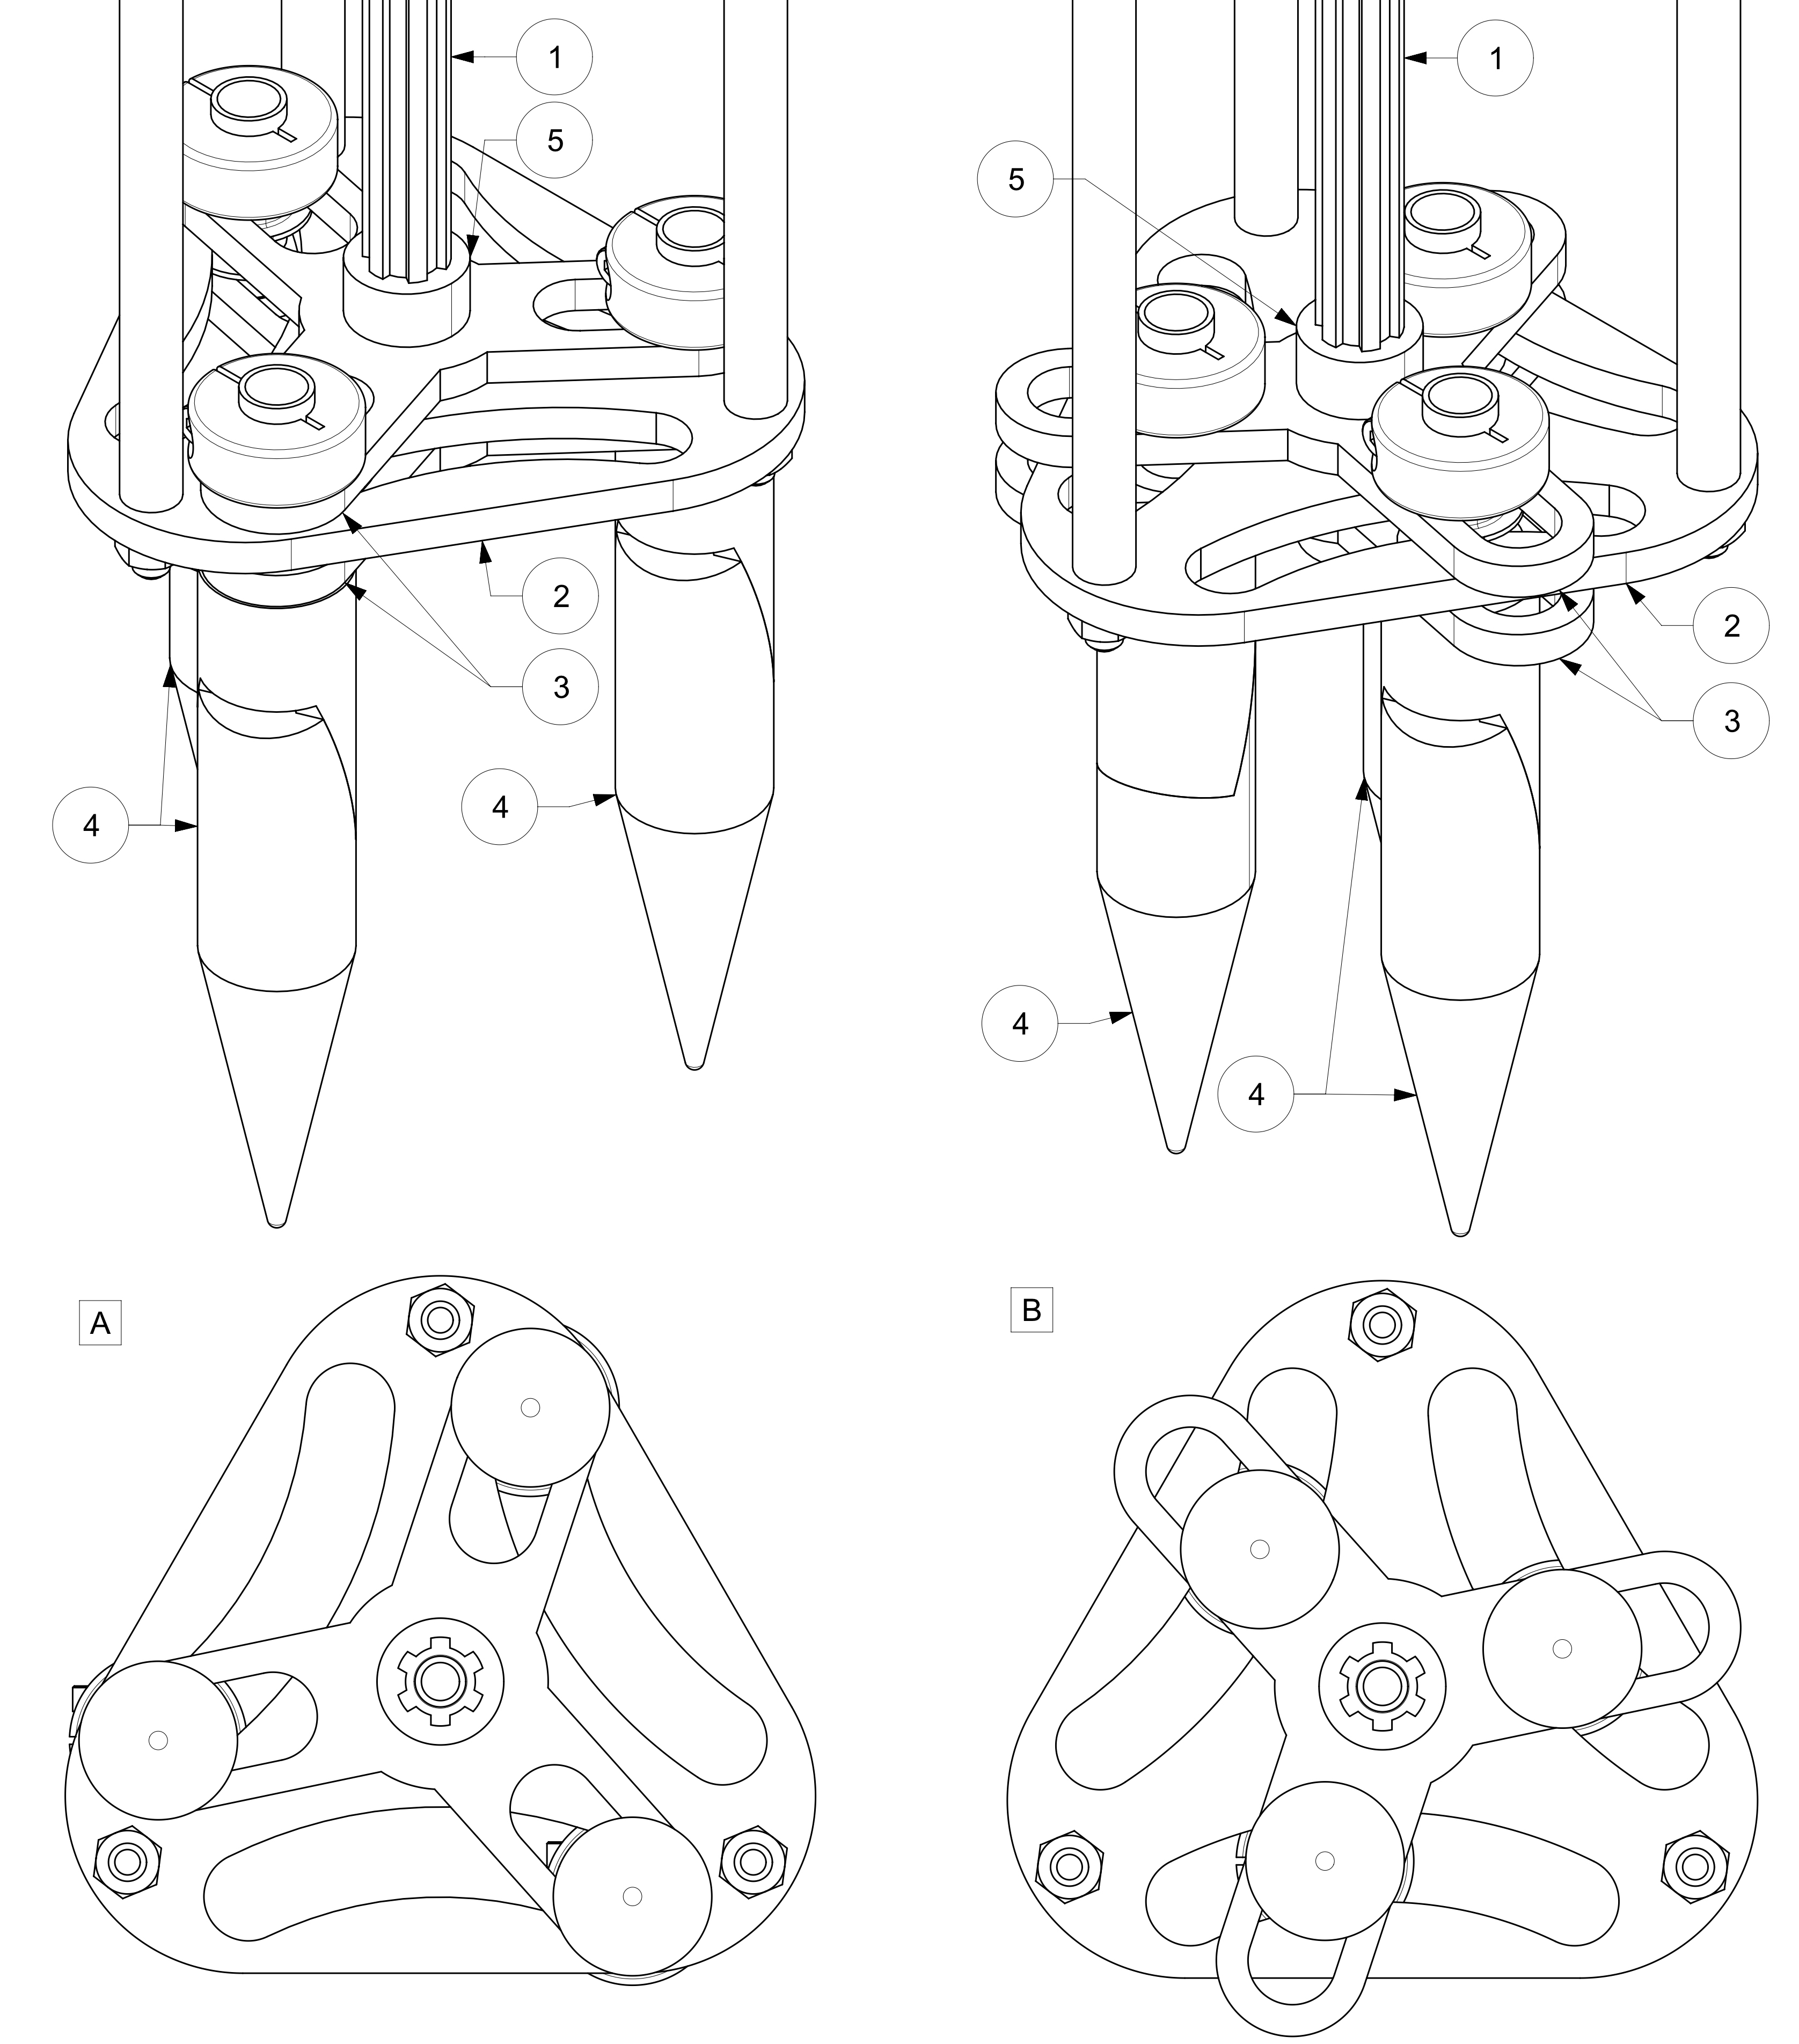
\includegraphics[draft=false,scale=0.53]{Illustrationen/6-Umsetzung/motion_vm.jpg}
	\caption{Verstellung des Topfradius}
	\label{fig:motion_vm}
	\end{figure}

Wie schon erläutert, ist ein geringes Gewicht der beschleunigten Masse anzustreben. Gemäss Berechnungen soll die beschleunigte Masse maximal 1kg betragen. Um diese Anforderung zu erfüllen, werden die Kulissen (Punkte 2 und 3 aus Abb. \ref{fig:motion_vm}) aus 6mm dickem Aluminiumblech hergestellt.

\subsubsection{Prozessablauf}
\textit{(pro)} Genaue Spezifikationen für den Antrieb der Verstellmechanik zu definieren stellte sich als schwierig heraus. Da die einzigen Drehmomente, welche dem Antrieb entgegenwirken, auf Reibkräfte der Mechanik beruhen, welche schlecht geschätzt werden können. Eine weitere Herausforderung bergen die kleinen Winkeländerungen an der Antriebswelle des Motors (der ganze Bewegungsraum von Anschlag zu Anschlag beträgt ca. 100°). Um solch kleine Winkeländerungen präzise fahren zu können wird ein DC Getriebemotor von Pololu mit einer Getriebeübersetzung von 378:1 verwendet.  Die Spezifikationen, sowie die Begründung für die Wahl dieser Antriebstechnik sind in Kapitel \ref{kap:Evaluation_der_Komponenten} erläutert.\\
Der Prozessablauf zur Initialisierung sowie das Einstellen verschiedener Topfgrössen ist in Abb. \ref{fig:Prozessablauf_Verstellmechanik} illustriert. Wie bei der Setzeinheit wird die Verstellmechanik durch das Anfahren eines mechanischen Anschlags initialisiert. Die verschiedenen Topfgrössen von 9cm... 14cm können durch fahren einer relativen Schrittweite zum Anschlag eingestellt werden.

\begin{figure}[H]
	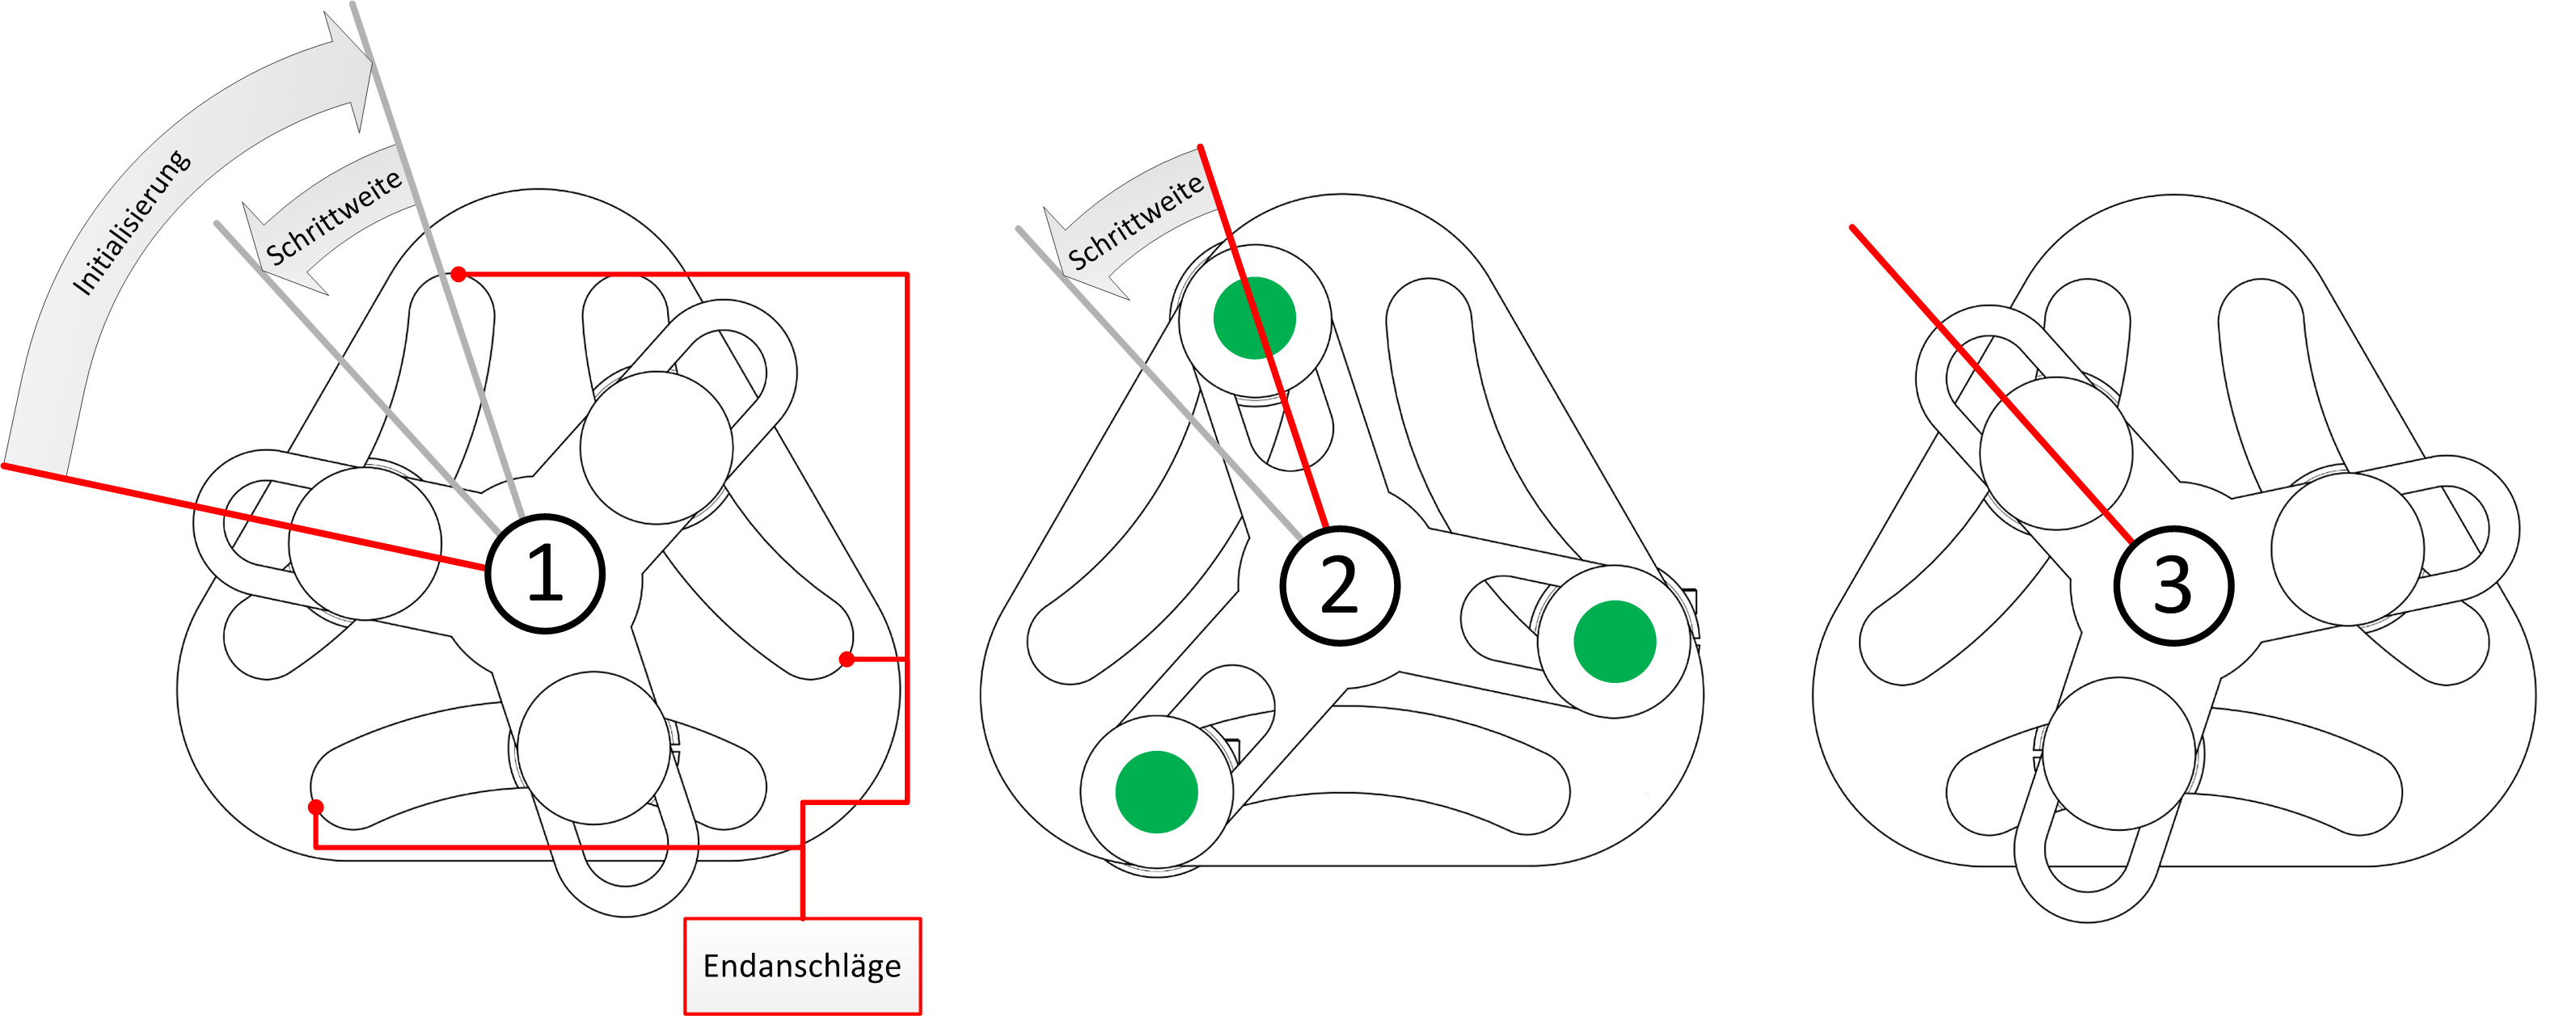
\includegraphics[width=1\textwidth]{Illustrationen/6-Umsetzung/Prozessablauf_Verstellmechanik.png}
	\caption{Prozessablauf der Verstellmechanik}
	\label{fig:Prozessablauf_Verstellmechanik}
\end{figure}

Der Prozess wurde in drei Etappen unterteilt welche mit den Ziffern 1... 3 nummeriert sind. Im folgenden Abschnitt werden die drei Etappen erläutert:

\begin{enumerate}
	\item Nach einem Neustart der Maschine befindet sich die Verstellmechanik in einer unbekannten Position. Um die absolute Position der Verstellmechanik zu ermitteln wird diese an die mechanischen Endanschläge der Führungskullise bewegt. Durch die Erhöhung des Laststroms wird der Endanschlag vom uC erkannt.
	\item In dieser Etappe befindet sich die Verstellmechanik an den Endanschlägen. Dies wurde durch grüne Kreise, an den jeweiligen Punkten wo die Mechanik den Endanschlag berührt, gekennzeichnet.
	\item Durch bewegen der Verstellmechanik, um eine definierte Schrittweite relativ zum Endanschlag, können nun die verschiedenen Setzradien eingestellt werden. Aufgrund der Form der Führungskulisse ergeben sich jeweils zwei Positionen, links und rechts vom kleinsten Setzradius, für die Topfgrössen 11cm, 12cm, 13cm und 14cm.
\end{enumerate}

Die Parameter für die Schrittweiten der jeweiligen Setzradien werden im Kapitel Inbetriebnahme (\ref{sec:Inbetriebnahme_Verstellmechanik}) behandelt.
\subsection{Stechdorn}
\textit{(ygu)} Der Stechdorn hat die Aufgabe ein Setzloch durch Verdrängung der Topferde auszuheben und anschliessend die fallenden NemaCaps ins Setzloch zu leiten. Dabei wurde bewusst auf einen gelochten Stechdorn verzichtet, um das Risiko von Verstopfungen zu vermeiden. Mit der realisierten Konstruktion ist diese Gefahr eliminiert. 
\subsubsection{Aufbau}
Der Stechdorn besteht aus mehreren Teilen, wobei diese über eine lineare Führung (Punkt 5 in Abbildung \ref{fig:details_stechdorn}) verbunden sind. Dabei wird das Haupt (1) an der Verstellmechanik montiert und macht die Translation der Setzeinheit mit. Sobald der untere Teil (2, 3) in die Topferde einsticht, fährt die Spitze an den oberen Anschlag der Führung (Detail A). Bei der Bewegung zurück nach oben, öffnet sich die Spitze wieder und das NemaCaps kann durch den Kanal (8) ins ausgehobene Setzloch fallen (Detail B). Diese Bewegung soll nur durch die Gewichts- sowie Trägheitskraft der Spitze ausgelöst werden. Falls die Spitze zu leicht ist, um sich durch die Bewegung zu öffnen, kann der Hohlraum der Spitze mit Blei aufgefüllt werden. Dafür ist ein Füllloch (4) vorgesehen, welches mit einer Madenschraube M6 verschlossen wird. Folgende Überlegungen geben die Lage der linearen Führung vor:

\begin{itemize}
	\item Die lineare Führung soll möglichst parallel zur Bewegungsachse der Setzeinheit verlaufen, sodass möglichst keine Radialkräfte auf den Dorn wirken.
	
	\item Wiederum muss eine seitliche Öffnung der Spitze soweit geschehen, dass die Öffnung (9) frei über dem Setzloch steht (Detail B) und ein freier Fall des NemaCaps möglich ist.
	
	\item Der maximale Weg der Spitze in vertikaler Richtung beschränkt durch die maximale Hublänge der Spindel. Dabei ist der Abstand A in den Berechnungen (vgl. Anhang: \textit{Auslegung Spindel}) mit 15mm angenommen. Die Umsetzung überschreitet diese Annahme um 1mm, bewegt jedoch im angemessenem Rahmen.
\end{itemize}

\begin{figure}[H]
	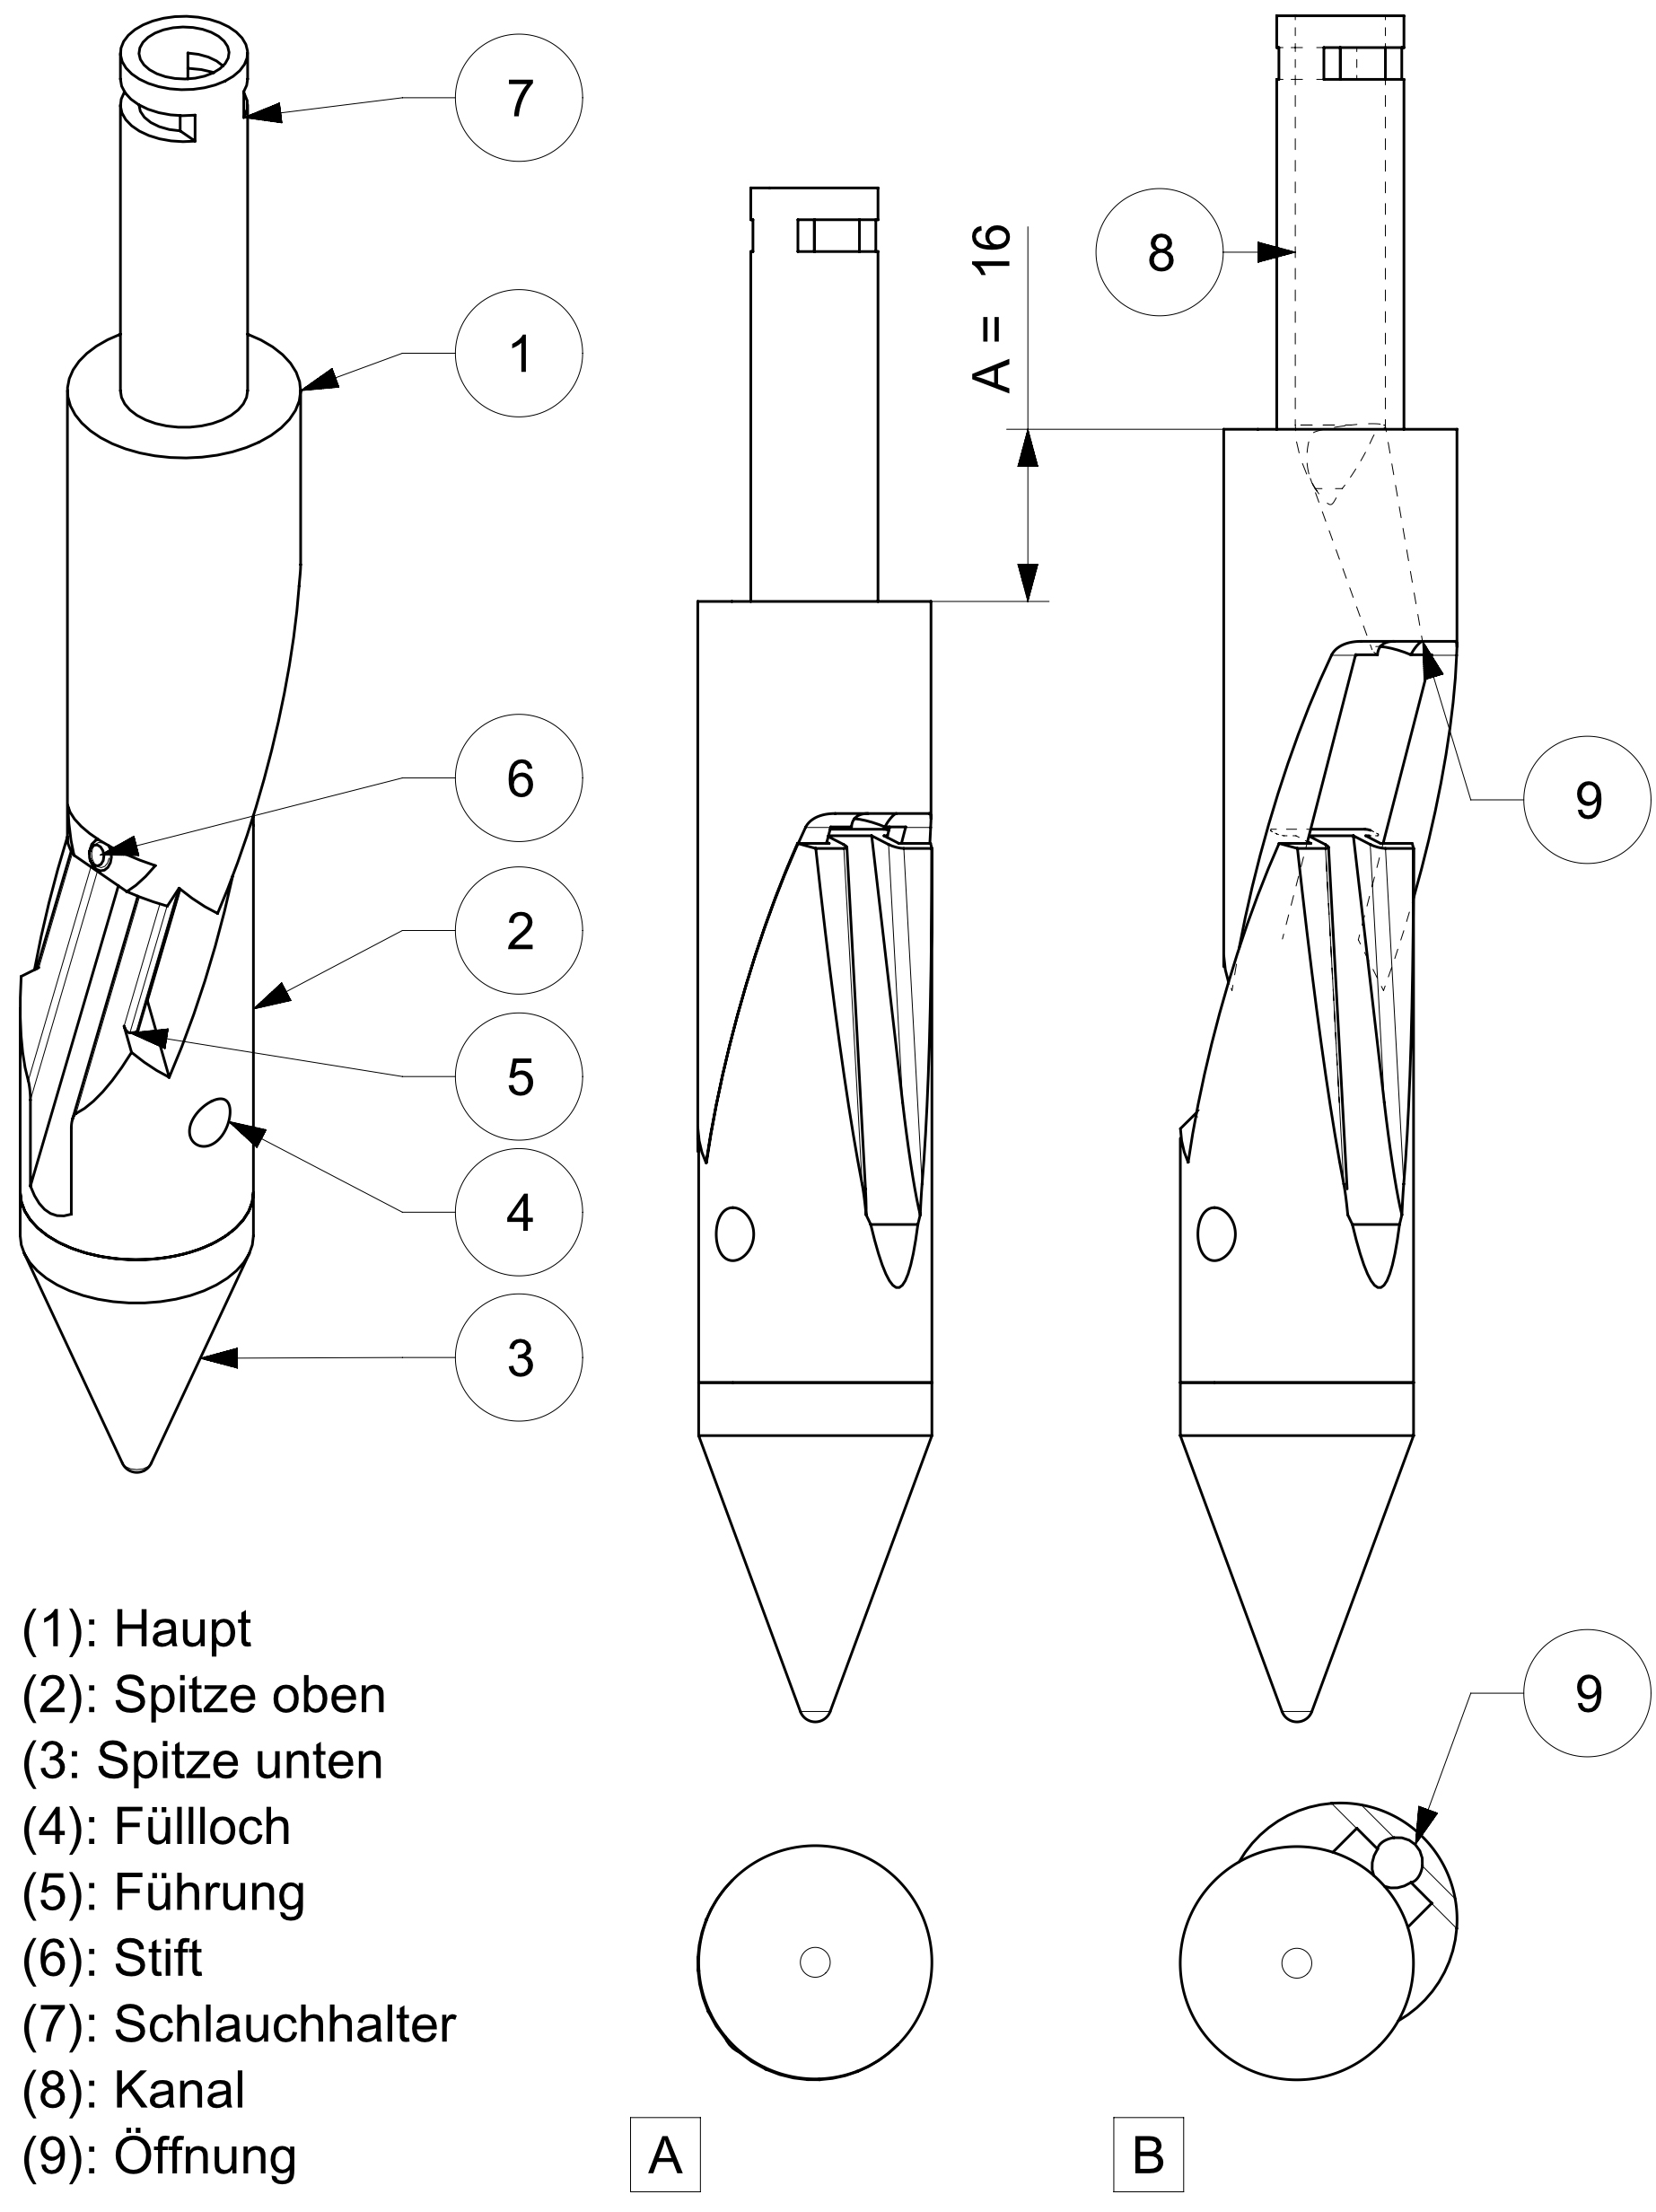
\includegraphics[width=1\textwidth]{Illustrationen/6-Umsetzung/details_stechdorn.jpg}
	\caption{Übersicht des Stechdorns}
	\label{fig:details_stechdorn}
\end{figure}




\subsubsection{Haupt}
Das Haupt des Stechdorns nimmt neben der linearen Führung der Spitze noch folgende Aufgaben wahr:
\begin{itemize}
	\item Es verbindet den Schlauch mit dem Stechdorn. Dafür kann der Schlauch oben eingeführt werden und am Schlauchhalter (Punkt 12 in Abbildung \ref{fig:details_haupt}) mit einem Kabelbinder montiert werden.
	
	\item Es lenkt das fallende NemaCap mit dem Kanal (8) zur vorgesehen Öffnung und dient somit der Platzierung.
	
	\item Mit der Anbringung eines Stiftes (13) wird der untere Anschlag der Führung gewährleistet. 
\end{itemize}

	\begin{figure}[H]
	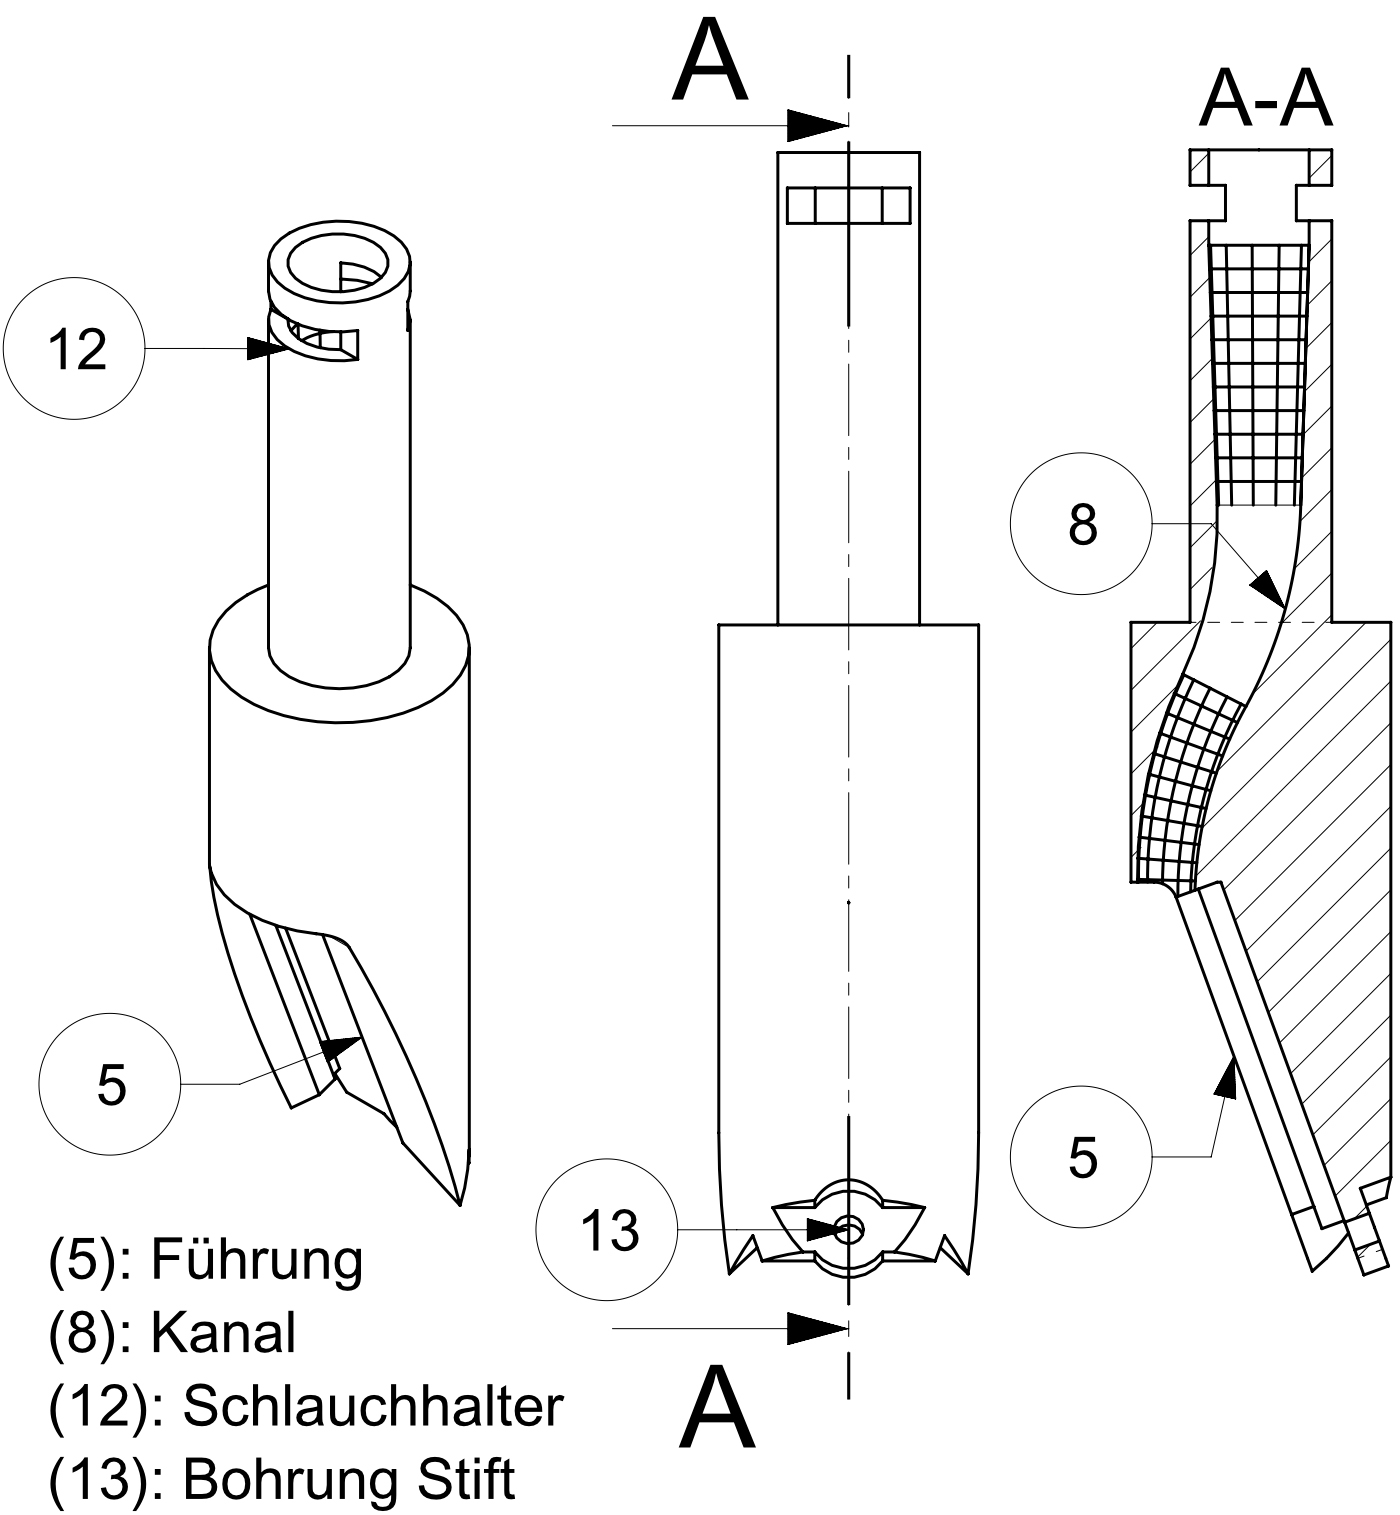
\includegraphics[width=0.8\textwidth]{Illustrationen/6-Umsetzung/details_haupt.jpg}
	\caption{Details zum Haupt}
	\label{fig:details_haupt}
	\end{figure}

\subsubsection{Spitze oben}
\label{spitzeoben}
An der Spitze oben sind folgende konstruktive Überlegungen hervorzuheben:
\begin{itemize}
	\item Die lineare Führung ist als breites T-Profil umgesetzt (Detail A in Abbildung \ref{fig:details_spitze_oben}). Dabei ist der Steg 1.8mm dick (Mass E). Als Spielmass zwischen beiden Führungsteilen wird in alle Richtungen 0.25mm verwendet.
	
	\item Bei ausgefahrener Spitze beträgt die verbleibende Länge der Führung 11mm (Mass D). Gemäss betreuendem Dozenten (Marco De Angelis) ist das Verhältnis p von Stegdicke zu verbleibender Länge essentiel bei der Realisation von linearen Führungen dieser Art. Ideal ist ein Verhältnis von 8 ... 10 anzustreben. in diesem Fall beträgt das Verhältnis p:
	
	\begin{equation}
	p=\frac{verbleibende Fuehrung}{Stegdicke}=\frac{D}{E}=\frac{11mm}{1.8mm}=6.11
	\end{equation}
		
	Ob ein Verhältnis von 6.1 für eine funktionierende Führung ausreicht, wird die Inbetriebnahme zeigen. Allenfalls müssen diese Parameter angepasst werden.
	
	\item Da die Spitze direkt an der Topferde ausgesetzt ist, muss mit Rückständen von Erdpartikel gerechnet werden. Dabei ist die Führung ein sensitiver Teil, deren Funktion bei Kontakt mit Erdpartikeln beeinträchtigt werden kann. Um das Risiko zu mindern, wurden vorbeugende Massnahmen in der Konstruktion berücksichtigt. Ein Auslauf der Führung (11) und zwei Fasen (10) sollen die Ansammlung von Erdpartikeln verhindern.
	\end{itemize}
	\begin{figure}[H]
	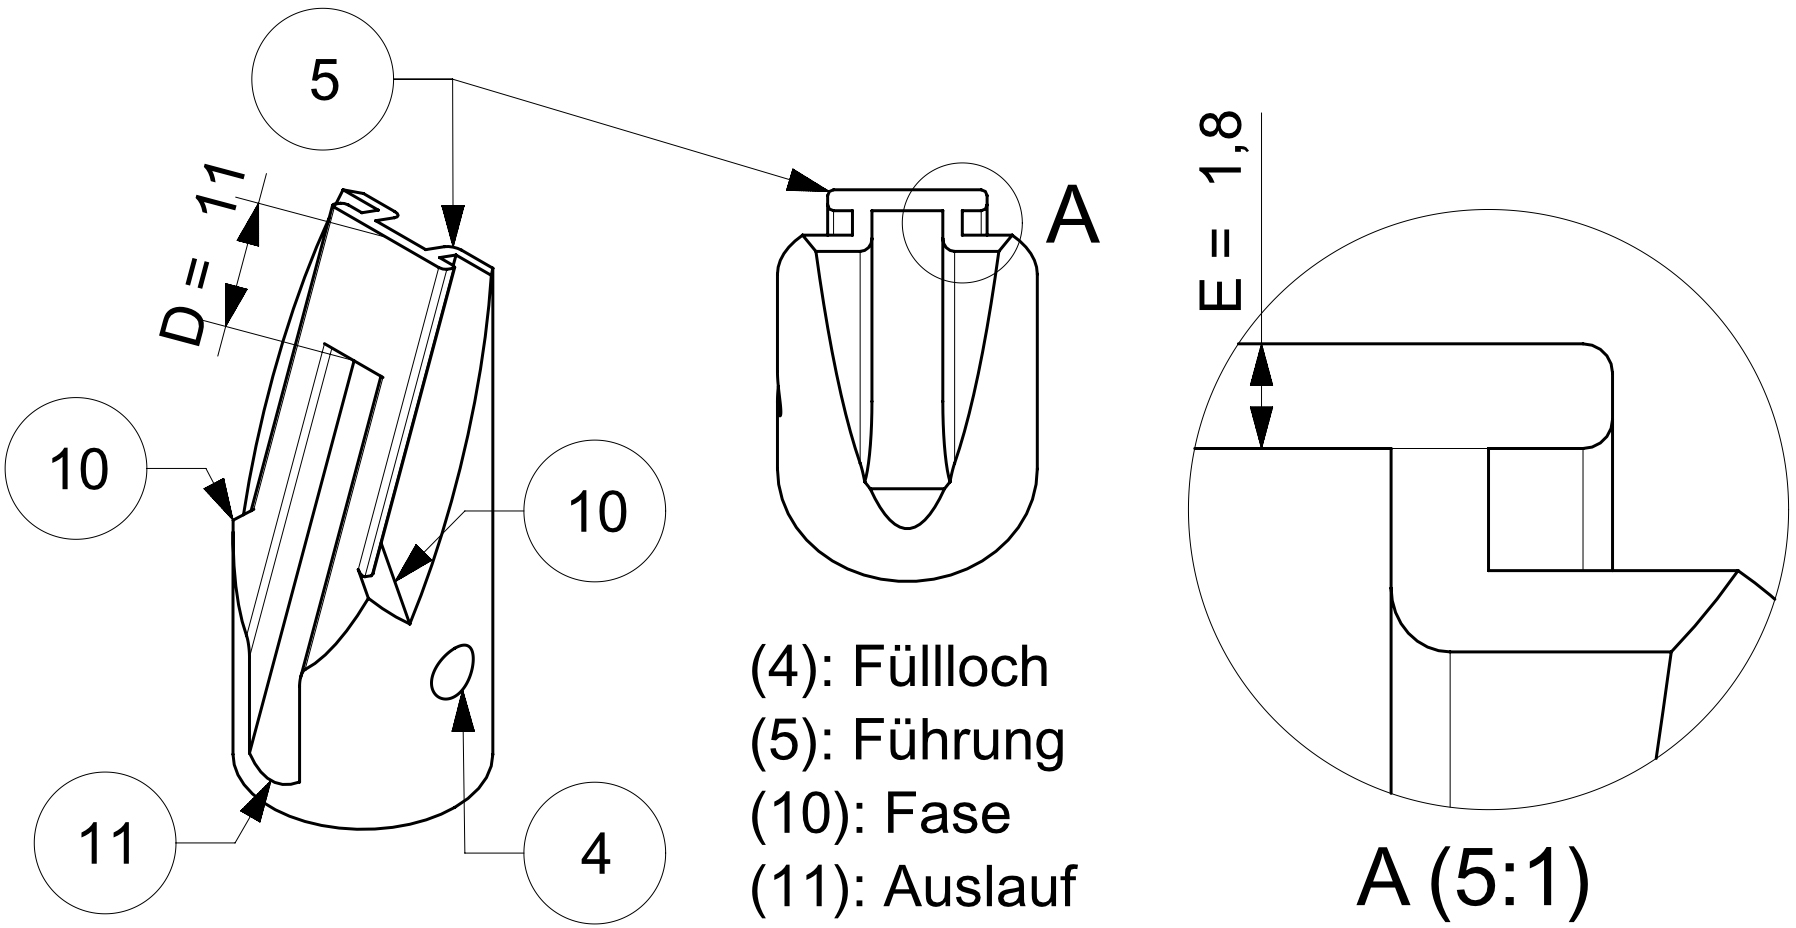
\includegraphics[scale=1.0]{Illustrationen/6-Umsetzung/details_spitze_oben.jpg}
	\caption{Details Spitze oben}
	\label{fig:details_spitze_oben}
	\end{figure}

\subsubsection{Schlauch}
Für den Transport der NemaCaps zwischen Vereinzelung und Stechdorn wird die Gravitation verwendet. Dabei werden die fallenden NemaCaps durch einen Pneumatikschlauch geleitet. Weiter stellt der Schlauch sicher, dass eine flexible Verbindung zum bewegten Stechdorn existiert. In der Pneumatik sind folgende Schlauchdimensionen gängig \cite{camozzi}:
\newline
\begin{table}[H]
\begin{tabular}{|c|c|}
	\hline 
	Aussendurchmesser D [mm] & Innendurchmesser d [mm] \\ 
	\hline 
	5 & 3 \\ 
	\hline 
	6 & 4  \\ 
	\hline 
	8 & 6 \\ 
	\hline 
	10 & 8  \\ 
	\hline 
\end{tabular}
	\caption{gängige Schlauchdimensioen}
	\label{tab:Schlauchdimensioen}
\end{table}

Für die Wahl der Schlauches stehen sich zwei widersprüchliche Aspekte gegenüber:
\begin{itemize}
	\item NemaCaps haben einen Durchmesser bis zu 3.6mm. Für einen freien Fall soll ein möglichst grosser Freiraum zur Schlauchinnenwand herrschen.
	
	\item Ein grosser Aussendurchmesser des Schlauches hat direkten Einfluss auf die Schlauchkupplungen sowie die Verstellmechanik. Dadurch werden diese Komponenten grösser. Der Lochabstand der Lochmaske steigt an und die Verstellmechanik muss grösser dimensioniert werden. Dies bedeutet mehr translatorisch beschleunigte Masse durch die Spindel. Somit ist hierfür die Wahl eines kleinen Schlauchdurchmessers vorteilhaft.
\end{itemize}
Dieser Zielkonflikt beider Aspekte bedeutet, dass die optimale Wahl des Schlauches ein Kompromiss sein muss. Daher wird ein Schlauch mit den Dimensionen 8/6 (D/d) verwendet.
\newline
Die Flexibilität wird durch das Material massgebend beeinflusst. Da keine Herstellerangaben dafür verfügbar sind, werden die Materialien Polyurethan sowie Polyamid (Nylon) für die Inbetriebnahme bestellt und dort miteinander verglichen.
\newpage
\subsection{Fertigungsverfahren und Material}
Das gewählte Fertigungsverfahren sowie verwendete Material beeinflusst die Charakteristik eines Teils massgeblich. Aufgrund der Relevanz wird diesen Thema ein Unterkapitel gewidmet. Relevante Überlegungen betreffend Fertigungsverfahren und Material werden erläutert und deren Wahl begründet.

\subsubsection{Lasertrennverfahren}
Für Einfache Teile mit zweidimensionaler Kontur bietet sich Lasertrennen als Verfahren an. Beim Lasertrennen wird durch das Fokussieren von gebündelten Laserstrahlen und einem Schneidgas am Werkstück eine Schnittfuge erzeugt \cite{laser}. Durch das zweidimensionale Bewegen des Fokus wird eine Kontur geschnitten. Vorteilhaft am Lasertrennen ist:

\begin{itemize}
	\item Beliebige zweidimensionale Konturen können realisiert werden.
	
	\item Durch die konsequente Verwendung vom gleichen Material sowie einem Miniumum an Blechdicken können Umrüstzeiten eingespart werden. Dies hat direkt positiven Einfluss auf die Kosten.
	
	\item Die Fertigungsunterlagen können direkt aus dem CAD als .DXF-Datei exportiert und am Hersteller gesendet werden. 
\end{itemize}
Folgende Teile werden mit dem Lasertrennverfahren hergestellt:

\begin{table}[H]
\begin{tabular}{|c|c|c|c|}
	\hline 
	Stück & Dicke [mm] & Verwendung & Einheit \\ 
	\hline 
	4x & 6 &Montageplatten & Setzeinheit \\ 
	\hline 
	2x & 6 & bewegte Montageplatten & Setzeinheit \\ 
	\hline 
	3x & 6 & Kulissen & Verstellmechanik \\ 
	\hline 
	1x & 6 & Montageplatte & Vereinzelung \\ 
	\hline 
	2x & 6 & Leitbleche  & Vereinzelung \\ 
	\hline 
	1x & 6 & Deckel & Vereinzelung \\ 
	\hline 
	1x & 4 & Lochmaske & Vereinzelung  \\ 
	\hline 
\end{tabular}
	\caption{Teile die mittels Lasertrennenverfahren hergestellt werden}
	\label{tab:lasertrennen}
\end{table} 
Für das Funktionsmuster wird konsequent 6mm dickes Aluminium-Blech verwendet. Die Wahl der Dicke und des Materials wird wie folgt begründet:

\begin{itemize}
	\item Ein Teil der gelaserten Bleche wird für die Setzeinheit verwendet. Für den bewegten Teil ist es zentral, dass möglichst wenig Masse beschleunigt wird. Daher ein Werkstoff mit geringer Dichte verwendet.
	
	\item Durch die Verwendung von 6mm dickem Blech, können die Montageplatten direkt in der Nut der Kanya Profile montiert werden.
\end{itemize}

Einzig für die Lochmaske wird 4mm dickes Aluminium-Blech verwendet, da diese Dicke für die Abstreifung von überschüssigen NemaCaps zentral ist (vgl. Kapitel \ref{lochmaske}).

\subsubsection{Additive Fertigung}
Bestimmte Teile werden mittels Additiver Fertigung (Auch Rapid Prototyping oder umgspr. 3D-Drucken genannt) hergestellt. Eines dieser Verfahren ist das Fused Deposition Modeling (FDM). Dabei werden niedrigschmelzender Kunststoffe durch eine Düse extrudiert und in Lagen geschichtet \cite{fdm}. Durch die Schichtung der Lagen entsteht das konstruierte Bauteil. Für Folgende Teile wird FDM als Fertigungsverfahren gewählt:
\begin{table}[H]
\begin{tabular}{|c|c|c|c|l|}
	\hline 
	Stück & Verwendung & Einheit & Material & Kommentar \\ 
	\hline 
	3 & Stechdorn & Stechdorn & ABS & dreiteilige Komponente \\ 
	\hline 
	2 & Magnethalter & Vereinzelung & ABS & für Bajonettverschluss \\ 
	\hline 
	1 & Trommel & Vereinzelung & ABS & Maximal druckbarer Raum verwendet \\ 
	\hline 
\end{tabular} 
	\caption{Teile die mittels Fused Deposition Modeling (FDM) hergestellt werden}
	\label{tab:fdm}
\end{table} 
Durch Additive Fertigung können verschiedenste Funktionen in einem Teil vereinigt werden (vgl. Kap.\ref{sec:Vereinzelung}, Trommel). Durch diese Integralbauweise werden Teile mit komplexer Geometrie herstellbar. Auch können kleine Teile in kurzer Zeit mit individuellen Anpassungen reproduziert werden. Dieser Vorteil wird beim Stechdorn genutzt. Für das Spielmass der linearen Führung wird durch zielgerichtetes Ausprobieren iterativ das richtige Mass gefunden. Diese Vorteile sind ausschlaggebend, dass FDM als Fertigungsverfahren für die genannten Bauteile gewählt wird.
\newline
Als Material wird der Thermoplast ABS verwendet. Dabei ist die geringe Dichte des Thermoplast vorteilhaft für den Stechdorn, da eine geringes Gewicht der Setzeinheit angestrebt wird.
\newline

Eine fertigungstechnische Einschränkung ergibt sich durch den druckbaren Raum des 3D-Druckers. Der interne 3D-Drucker der HSLU T\&A hat einen druckbaren Raum von 200mm x 200mm x 300mm. Dadurch ist der Aussendurchmesser der Trommel auf maximal 200mm beschränkt und kann nicht grösser gestaltet werden (vgl. Kap. \ref{sec:Vereinzelung}).

\begin{figure}[H]
	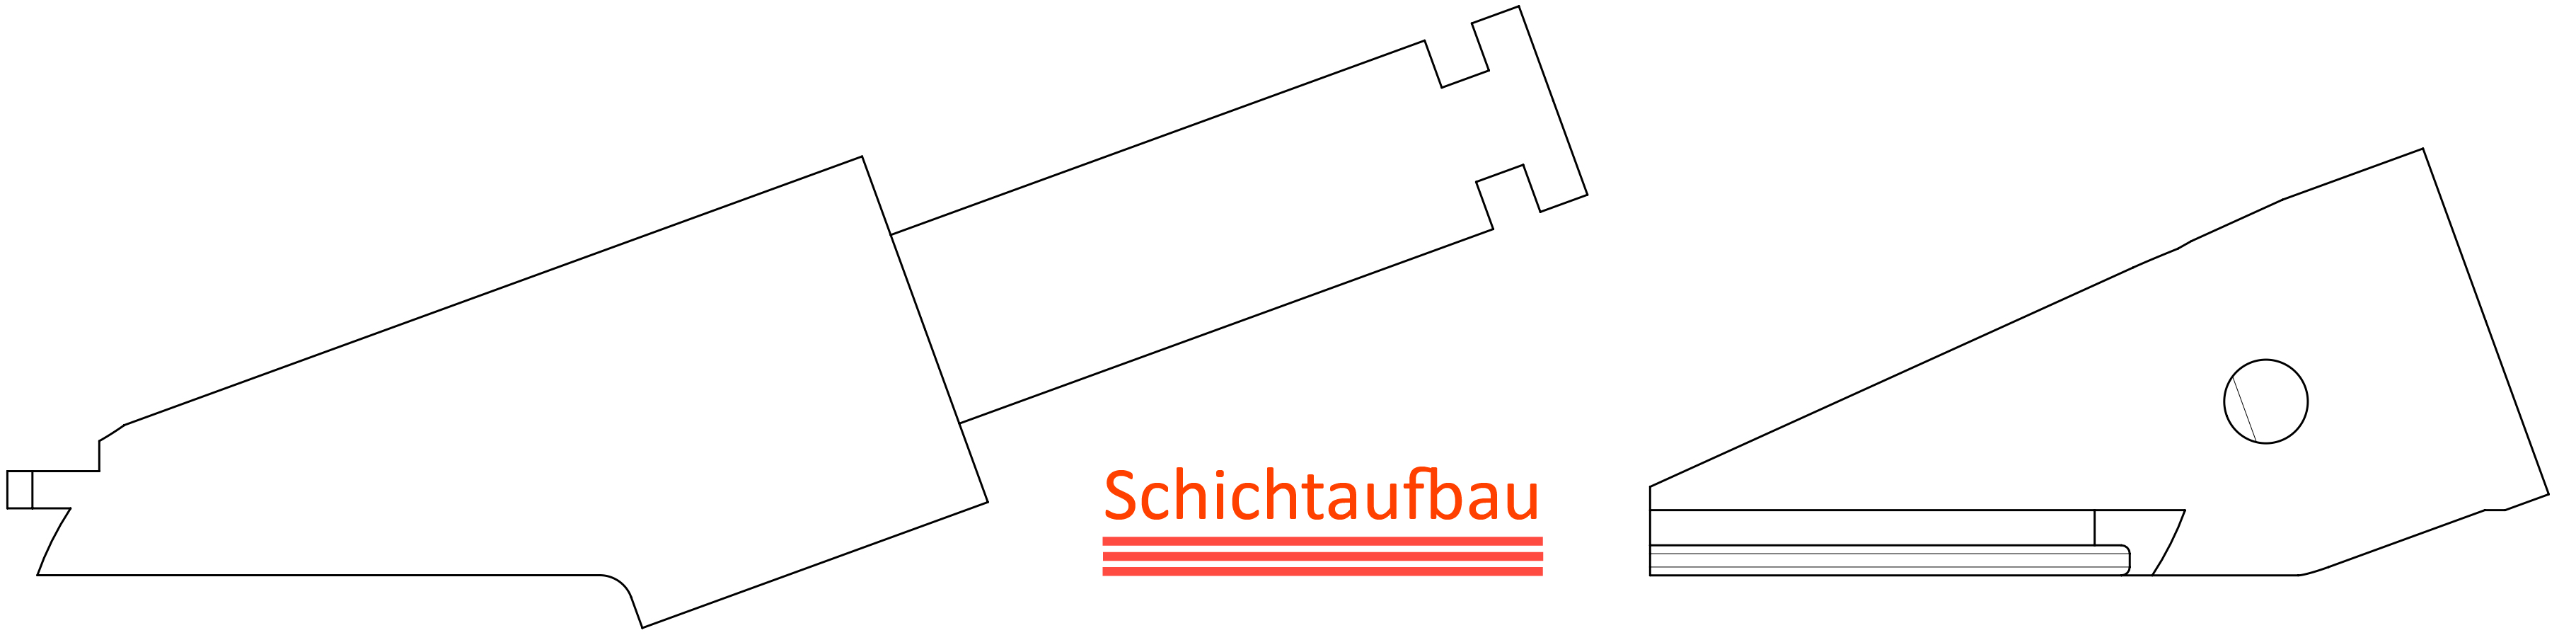
\includegraphics[scale=0.115]{Illustrationen/6-Umsetzung/anordnung_fdm.jpg}
	\caption{Anordnung der Teile des Stechdorns im 3D-Drucker}
	\label{fig:anordnung_fdm}
\end{figure}
Für die Fertigung des Stechdorns werden die Teile so angeordnet, dass die extrudierten Lagen parallel zur linearen Führung aufgebaut werden. So ist gewährleistet, dass entlang der Führung keine zusätzlichen Unebenheiten auftreten die den Widerstand erhöhen.
\subsection{Mainboard PCB}
\textit{(pro)} Um die Elektronik Komponenten auf übersichtliche und zuverlässige Weise miteinander zu verknüpfen wurde ein 2-Lagiges PCB designt welches als Prototyp an der HSLU gefertig werden kann. Durch ein PCB wird der Verdrahtungsaufwand zwischen den Komponenten auf ein Minimum reduziert. In den folgenden Unterkapiteln wird das Schema, die verwendeten Elektronik Bauteile und das Layout des Mainboard PCBs erklärt.
\subsubsection{FRDM-KL25Z Header}
Das Mainboard PCB verbindet sämtliche Elektronik Komponenten miteinander. Das Herzstück bildet dabei das Mikrocontroller Board FRDM-KL25Z von NXP, welches über Stiftleisten auf das Mainboard aufgesteckt wird. Es verfügt über einen 32-bit ARM Cortex M0+ Mikrocontroller mit einer Taktrate von 48MHz, 128KB Flash und 16KB RAM. In der folgenden Tabelle werden die Signale welche vom FRDM-Board zur Verfügung gestellt werden aufgeführt. Die Spalten der Tabelle sind wie folgt zu lesen: \textbf{CON} ist der Stecker mit der jeweiligen Pin Nummer, \textbf{Port} beschreibt den Pin des uC, \textbf{Mapping} gibt an für was der Port des uC verwendet wird und \textbf{Funktion} beschreibt die Verwendung des uC Pins auf dem Mainboard PCB.

% Table generated by Excel2LaTeX from sheet 'FRDM-KL25z Port Mapping'
\begin{table}[H]
	\scriptsize
	\centering
	\caption{FRDM-KL25Z Port Mapping}
	\begin{tabular}{|r|r|r|r|l|l|r|l|}
		\hline
		\multicolumn{1}{|l|}{\textbf{CON}} & \multicolumn{1}{l|}{\textbf{Port}} & \multicolumn{1}{l|}{\textbf{Mapping}} & \multicolumn{1}{l|}{\textbf{Funktion}} & \textbf{CON} & \textbf{Port} & \multicolumn{1}{l|}{\textbf{Mapping}} & \textbf{Funktion} \\
		\hline
		\multicolumn{1}{|l|}{J1 01} & \multicolumn{1}{l|}{PTC7} &       & \multicolumn{1}{l|}{NC} & J2 01 & PTC12 & \multicolumn{1}{l|}{Digital In} & BTN\_tiefer \\
		\hline
		\multicolumn{1}{|l|}{J1 02} & \multicolumn{1}{l|}{PTA1 } & \multicolumn{1}{l|}{UART0\_RX} & \multicolumn{1}{l|}{Bluetooth RX} & J2 02 & PTA13  & \multicolumn{1}{l|}{FTM1\_CH1} & Vibramotors 1 \\
		\hline
		\multicolumn{1}{|l|}{J1 03} & \multicolumn{1}{l|}{PTC0} & \multicolumn{1}{l|}{ADC0\_SE14} & \multicolumn{1}{l|}{IR-Sensor} & J2 03 & PTC13 & \multicolumn{1}{l|}{Digital In} & BTN\_höher \\
		\hline
		\multicolumn{1}{|l|}{J1 04} & \multicolumn{1}{l|}{PTA2 } & \multicolumn{1}{l|}{UART0\_TX} & \multicolumn{1}{l|}{Bluetooth TX} & J2 04 & PTD5  & \multicolumn{1}{l|}{Digital Out} & CSN nRF24L01+ \\
		\hline
		\multicolumn{1}{|l|}{J1 05} & \multicolumn{1}{l|}{PTC3} &       & \multicolumn{1}{l|}{NC} & J2 05 & PTC16 & \multicolumn{1}{l|}{Digital In} & BTN Vereinzeln \\
		\hline
		\multicolumn{1}{|l|}{J1 06} & \multicolumn{1}{l|}{PTD4 } & \multicolumn{1}{l|}{Digital Out} & \multicolumn{1}{l|}{DC\_OK} & J2 06 & PTD0  & \multicolumn{1}{l|}{Digital Out} & CE nRF24L01+ \\
		\hline
		\multicolumn{1}{|l|}{J1 07} & \multicolumn{1}{l|}{PTC4} &       & \multicolumn{1}{l|}{NC} & J2 07 & PTC17 & \multicolumn{1}{l|}{Digital In} & BTN Spindel runter \\
		\hline
		\multicolumn{1}{|l|}{J1 08} & \multicolumn{1}{l|}{PTA12 } & \multicolumn{1}{l|}{FTM1\_CH0} & \multicolumn{1}{l|}{Vibramotors 2} & J2 08 & PTD2  & \multicolumn{1}{l|}{SPI0\_MOSI} & nRF24L01+ \\
		\hline
		\multicolumn{1}{|l|}{J1 09} & \multicolumn{1}{l|}{PTC5} &       & \multicolumn{1}{l|}{NC} & J2 09 & PTA16  & \multicolumn{1}{l|}{Digital In} & BTN Spindel hoch \\
		\hline
		\multicolumn{1}{|l|}{J1 10} & \multicolumn{1}{l|}{PTA4 } & \multicolumn{1}{l|}{Digital Out} & \multicolumn{1}{l|}{Servo enable} & J2 10 & PTD3  & \multicolumn{1}{l|}{SPI0\_MISO} & nRF24L01+ \\
		\hline
		\multicolumn{1}{|l|}{J1 11} & \multicolumn{1}{l|}{PTC6} &       & \multicolumn{1}{l|}{NC} & J2 11 & PTA17  &       & NC \\
		\hline
		\multicolumn{1}{|l|}{J1 12} & \multicolumn{1}{l|}{PTA5 } & \multicolumn{1}{l|}{FTM0\_CH2} & \multicolumn{1}{l|}{ION enable} & J2 12 & PTD1  & \multicolumn{1}{l|}{SPI0\_SCK} & nRF24L01+ \\
		\hline
		\multicolumn{1}{|l|}{J1 13} & \multicolumn{1}{l|}{PTC10} & \multicolumn{1}{l|}{I2C1\_SDA} & \multicolumn{1}{l|}{LED Driver} & J2 13 & PTE31 & \multicolumn{1}{l|}{FTM0\_CH4} & Servo 3 \\
		\hline
		\multicolumn{1}{|l|}{J1 14} & \multicolumn{1}{l|}{PTC8 } & \multicolumn{1}{l|}{Digital Out} & \multicolumn{1}{l|}{Stop\_In} & J2 17 & PTD6  &       & NC \\
		\hline
		\multicolumn{1}{|l|}{J1 15} & \multicolumn{1}{l|}{PTC11} & \multicolumn{1}{l|}{I2C1\_SCL } & \multicolumn{1}{l|}{LED Driver} & J2 18 & PTE1  & \multicolumn{1}{l|}{UART1\_RX} & TMCM-1630 TX \\
		\hline
		\multicolumn{1}{|l|}{J1 16} & \multicolumn{1}{l|}{PTC9 } & \multicolumn{1}{l|}{Digital Out} & \multicolumn{1}{l|}{IRQ nRF24L01+} & J2 19 & PTD7  &       & NC \\
		\hline
		\multicolumn{1}{|l|}{J10 01} & \multicolumn{1}{l|}{PTE20} & \multicolumn{1}{l|}{ADC0\_SE0} & \multicolumn{1}{l|}{IR Sensor 2} & J2 20 & PTE0  & \multicolumn{1}{l|}{UART1\_TX } & TMCM-1630 RX \\
		\hline
		\multicolumn{1}{|l|}{J10 02} & \multicolumn{1}{l|}{PTB0 } & \multicolumn{1}{l|}{ADC0\_SE8} & \multicolumn{1}{l|}{IR Sensor 1} & J9 01 & PTB8  & \multicolumn{1}{l|}{Digital In} & BTN\_AUTO \\
		\hline
		\multicolumn{1}{|l|}{J10 03} & \multicolumn{1}{l|}{PTE21} &       & \multicolumn{1}{l|}{NC} & J9 03 & PTB9  & \multicolumn{1}{l|}{Digital In} & BTN\_14cm \\
		\hline
		\multicolumn{1}{|l|}{J10 04} & \multicolumn{1}{l|}{PTB1 } &       & \multicolumn{1}{l|}{Spare GPIO} & J9 05 & PTB10 & \multicolumn{1}{l|}{Digital In} & BTN\_13cm \\
		\hline
		\multicolumn{1}{|l|}{J10 05} & \multicolumn{1}{l|}{PTE22 } & \multicolumn{1}{l|}{UART2\_TX} & \multicolumn{1}{l|}{RoboClaw RX} & J9 07 & PTB11 & \multicolumn{1}{l|}{Digital In} & BTN\_12cm \\
		\hline
		\multicolumn{1}{|l|}{J10 06} & \multicolumn{1}{l|}{PTB2 } &       & \multicolumn{1}{l|}{Spare GPIO} & J9 09 & PTE2  & \multicolumn{1}{l|}{Digital In} & BTN\_11cm \\
		\hline
		\multicolumn{1}{|l|}{J10 07} & \multicolumn{1}{l|}{PTE23} & \multicolumn{1}{l|}{UART2\_RX} & \multicolumn{1}{l|}{RoboClaw TX} & J9 10 & P5V\_USB &       & NC \\
		\hline
		\multicolumn{1}{|l|}{J10 08} & \multicolumn{1}{l|}{PTB3 } &       & \multicolumn{1}{l|}{Spare GPIO} & J9 11 & PTE3  & \multicolumn{1}{l|}{Digital In} & BTN\_9cm \\
		\hline
		\multicolumn{1}{|l|}{J10 09} & \multicolumn{1}{l|}{PTE29} & \multicolumn{1}{l|}{FTM0\_CH2} & \multicolumn{1}{l|}{Servo 1} & J9 12 & GND   & \multicolumn{1}{l|}{GND} & GND \\
		\hline
		\multicolumn{1}{|l|}{J10 10} & \multicolumn{1}{l|}{PTC2} &       & \multicolumn{1}{l|}{Spare GPIO} & J9 13 & PTE4  &       & NC \\
		\hline
		\multicolumn{1}{|l|}{J10 11} & \multicolumn{1}{l|}{PTE30} & \multicolumn{1}{l|}{FTM0\_CH3} & \multicolumn{1}{l|}{Servo 2} & J9 14 & GND   & \multicolumn{1}{l|}{GND} & GND \\
		\hline
		\multicolumn{1}{|l|}{J10 12} & \multicolumn{1}{l|}{PTC1} &       & \multicolumn{1}{l|}{Spare GPIO} & J9 15 & PTE5  &       & Spare GPIO \\
		\hline
		&       &       &       & J9 16 & P5-9V\_VIN &       & 5VCC \\
		\hline
	\end{tabular}%
	\label{tab:FRDM_Port_Mapping}%
\end{table}%

Beim Design des Mainboard PCBs wurde darauf geachtet, dass möglichst viele GPIO Pins des FRDM-Boards genutzt werden. Deshalb wurde zusätzlich zu den in Abbildung \ref{fig:Blockschaltbild_Komponenten} aufgeführten Peripherien, ein Servo Interface mit drei Servo Anschlüssen und eine Buchsenleiste mit zusätzlichen GPIOs vorgesehen.

\subsubsection{Anschlüsse}
Die im vorhergehenden Kapitel beschriebenen Signale werden über Steckverbindungen auf das Mainboard geführt. Die Steckverbindungen sind in Abb. \ref{fig:Mainboard_3D} mit einer jeweiligen Beschriftungen illustriert. Die Anschlüsse welche nicht beschriftet sind gehören zum HMI und werden im Kapitel \ref{sec:Mainboard_HMI_Interface} behandelt. Für Signalleitungen und Speiseleitungen bis 2A werden JST Stecker der Serie PH mit 2, 3, 4 und 6 Pol verwendet. Diese haben ein schmales Rastermass von 2mm und eignen sich daher gut für kompakte PCB Anwendungen. Die 12V Speisung und das ION Motion Interface werden über 90° Phoenix Stiftleisten der Serie MSTBA geführt. Diese Stecker sind mit einem Nennstrom von 10A gemäss UL Zertifizierung zugelassen.

\begin{figure}[H]
	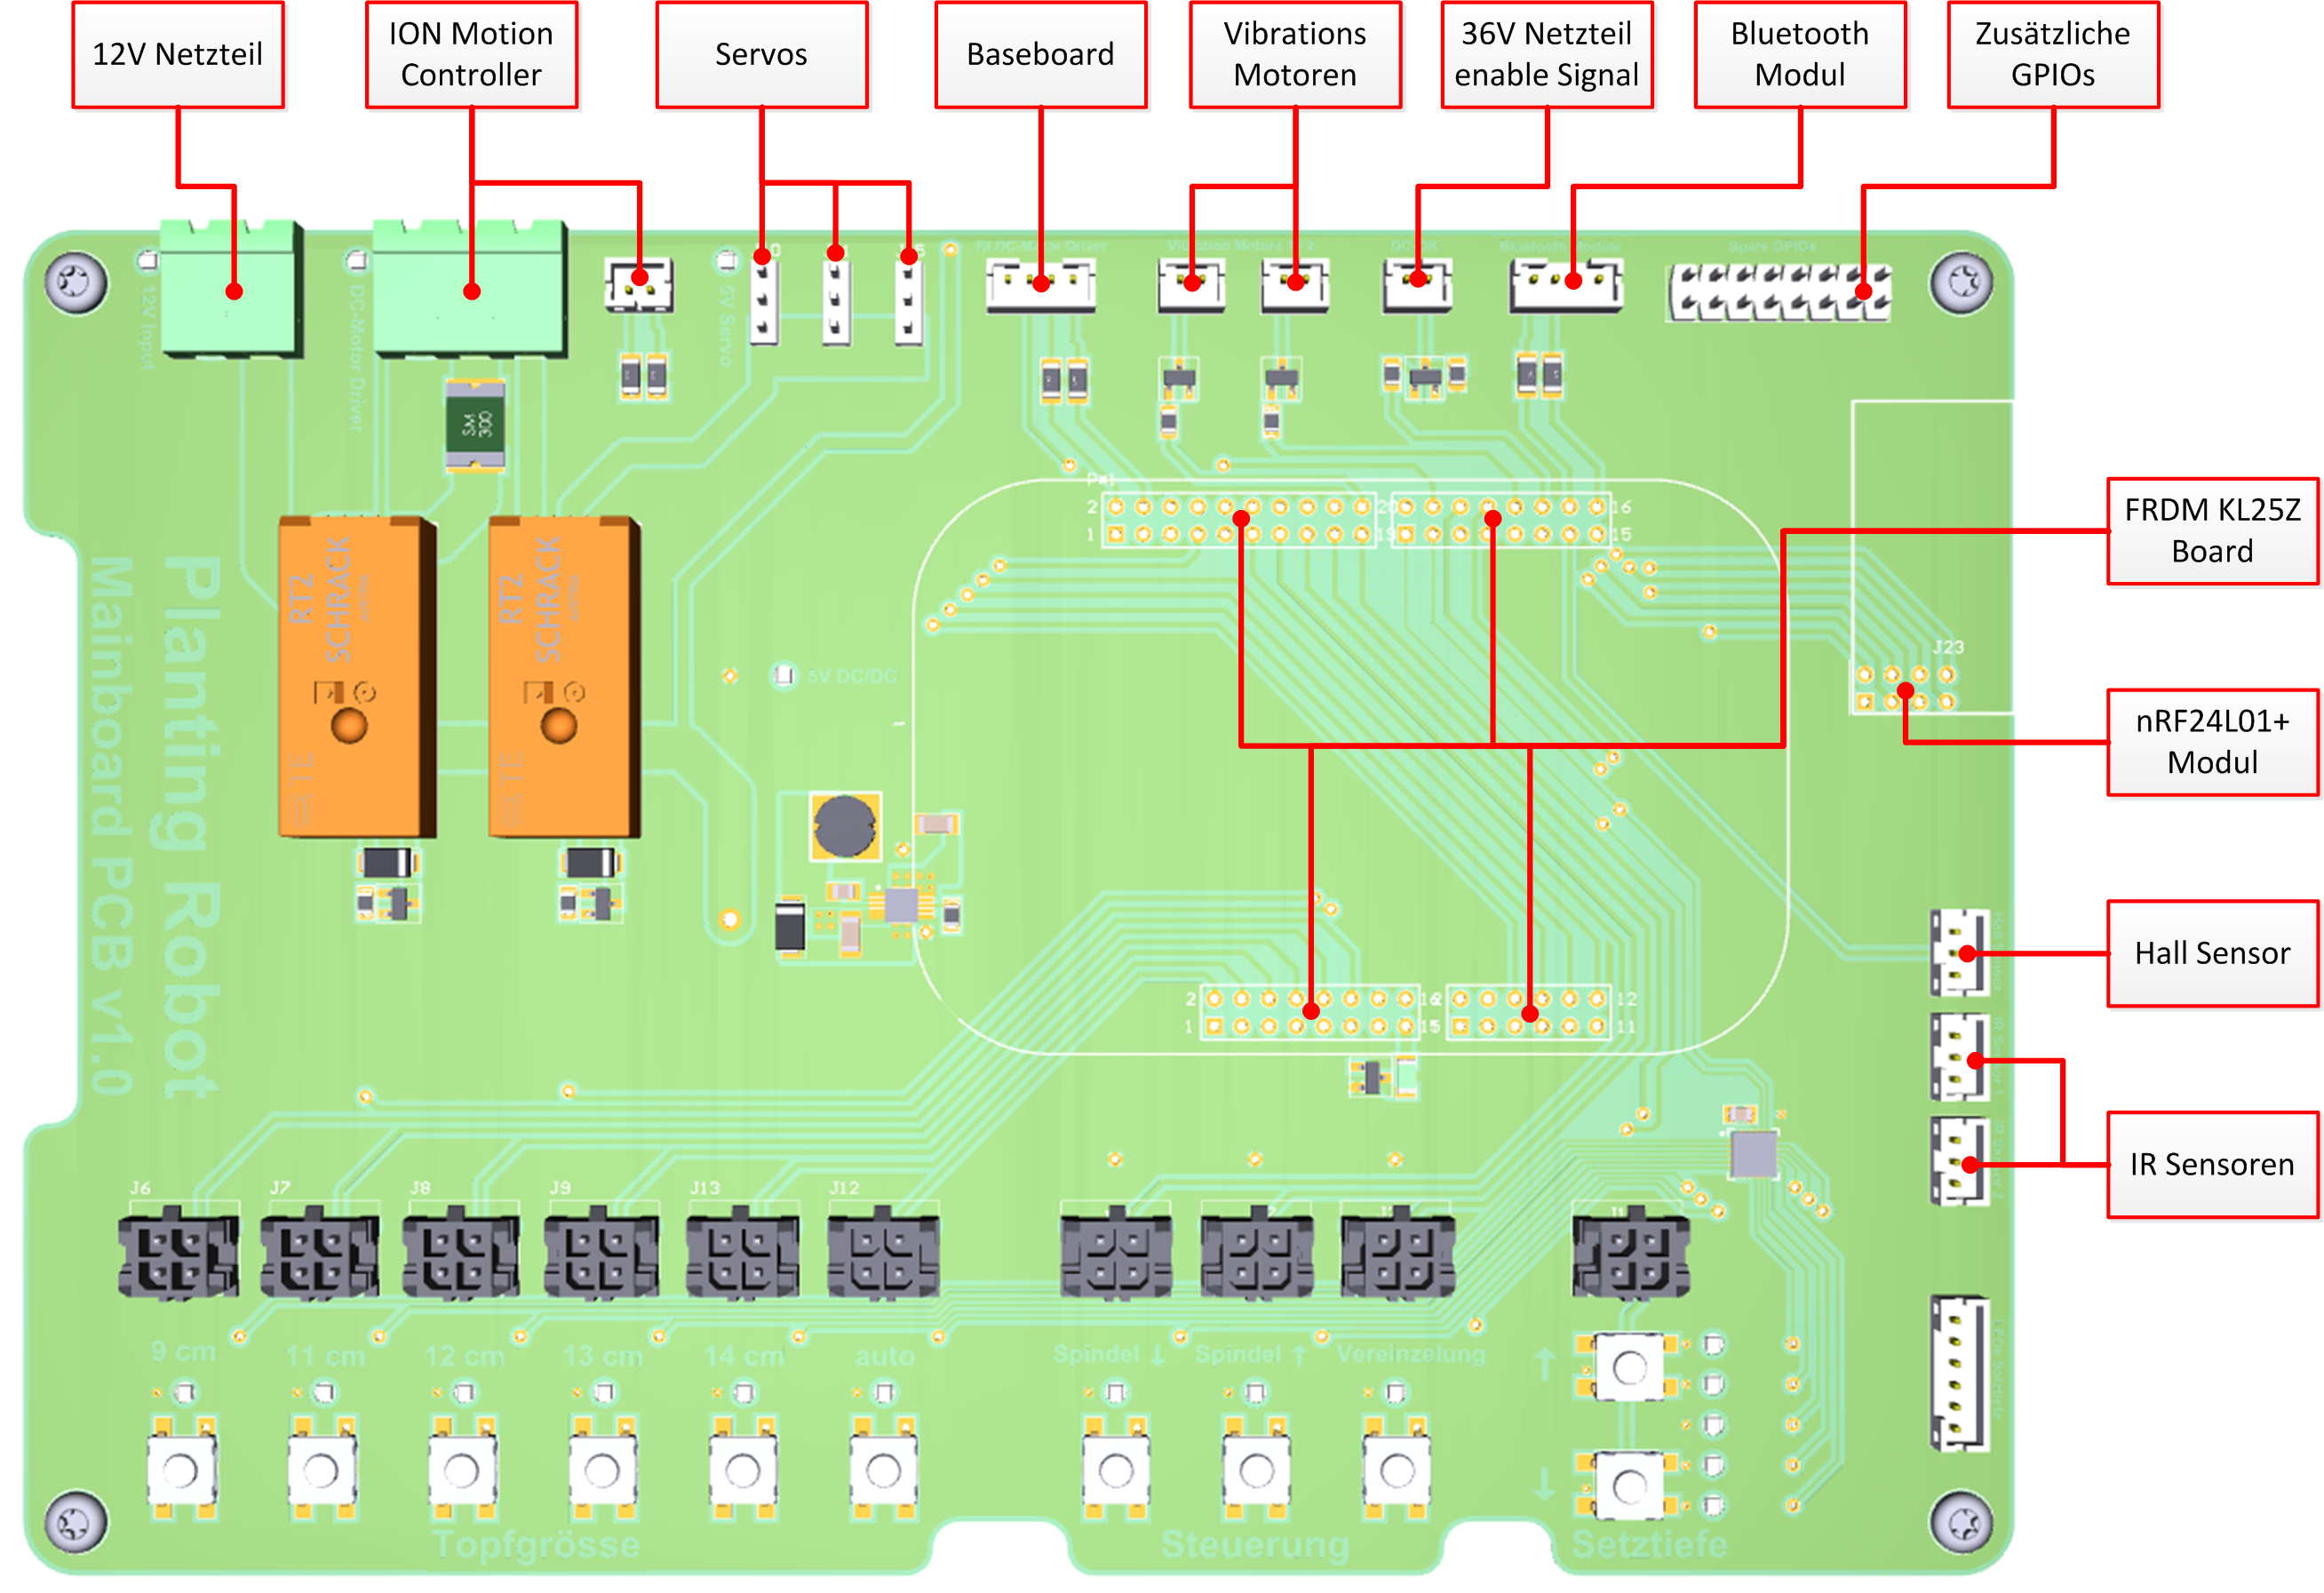
\includegraphics[width=1\textwidth]{Illustrationen/6-Umsetzung/Mainboard_PCB_Anschluesse.png}
	\caption{Mainboard PCB, Anschlüsse}
	\label{fig:Mainboard_3D}
\end{figure}

Um allfällig zusätzliche Peripherie mit dem FRDM-Board verbinden zu können, ist eine zweireihige 16P Stiftleiste mit 6 GPIO Ports, einer I$^{2}$C Schnittstelle, einem 5V und 12V Spannungspin vorgesehen. Des weiteren werden können das FRDM-Board und das nRF24L01+ Modul über Stiftleisten auf das Mainboard PCB gesteckt werden.

\subsubsection{Power Supply}
In Abb. \ref{fig:Schema_Mainboard_PowerSupply} ist der Power Supply Teil des Schemas vom Mainboard PCB abgebildet. Das Mainboard wird über das selbe 12V Netzteil mit Strom versorgt wie der ION Motion Motorcontroller. Um die Stromversorgung des Motorcontrollers schalten zu können wird diese über das Mainboard geführt. Auf dem Mainboard PCB befindet sich dann das Relais U3, welches vom uC gesteuert wird. Ebenfalls schaltbar ist die 5V Speisung des Servo Interfaces über das Relais U2. Dieses Spannungspotential wird vom ION Motion Controller abgegriffen. Dieser Verfügt über einen 5V Spannungswandler welcher bis zu 3A liefern kann. Die Speisung für den BLDC Motor kann über das DC$\_$OK Signal des 36V Netzteils geschalten werden. Das DC-OK Signal ist ein TTL Signal und wird deshalb über den Transistor Q1 vom uC geschaltet.

\begin{figure}[H]
	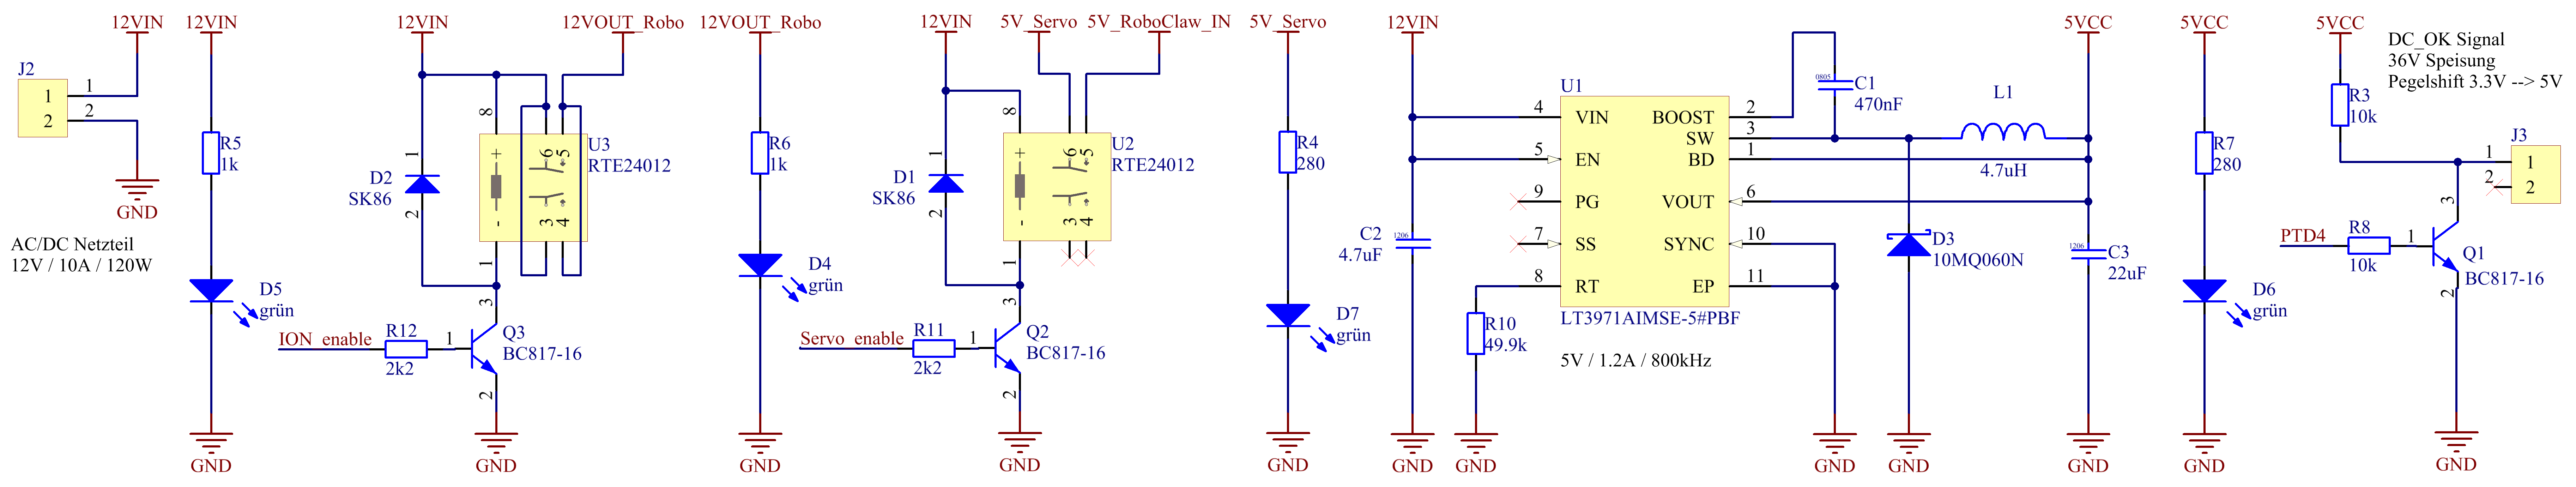
\includegraphics[width=1\textwidth]{Illustrationen/6-Umsetzung/Schema_Mainboard_PowerSupply.png}
	\caption{Schema Mainboard PCB, Power Supply}
	\label{fig:Schema_Mainboard_PowerSupply}
\end{figure}

Die Spannungsversorgung für das FRDM-Board, den LED Treiber, die Sensoren und die Vibrationsmotoren wird durch den DC/DC-Festspannungsregler LT3971 bereit gestellt. In der folgenden Tabelle sind die wichtigsten Daten des Buck Reglers ausgeführt:

% Table generated by Excel2LaTeX from sheet 'LT3971 Datasheet'
\begin{table}[htbp]
	\small
	\centering
	\caption{LT3971 Überblick Daten \protect\cite{LT3971_Datasheet}}
	\begin{tabular}{|l|ccc|r|}
		\hline
		\textbf{Parameter} & \multicolumn{1}{l}{\textbf{MIN}} & \multicolumn{1}{l}{\textbf{TYP}} & \multicolumn{1}{l}{\textbf{MAX}} & \textbf{Einheit} \\
		\hline
		Eingangsspannung &       &       & 38    & V \\
		\hline
		Ausgangsspannung & 4.93  & 5     & 5.07  & V \\
		\hline
		Ausgangsstrom &       &       & 1.2   & A \\
		\hline
		Schaltfrequenz & 0.2   &       & 2     & MHz \\
		\hline
		Wirkungsgrad &       & 85    &       & \% \\
		\hline
	\end{tabular}%
	\label{tab:LT3971_Datasheet}%
\end{table}%

Bei einem getakteten Spannungswandler sollte das Layout gemäss den Design Richtlinien des Herstellers erstellt werden. Dadurch wird garantiert, dass die Funktionalität und die EMV Eigenschaften der Schaltung auf einem hohen Niveau sind. Die Bauteilwerte der Schaltung wurden der typical application des Datenblatts entnommen. Der Buck Regler wird demanch mit einer Schaltfrequenz von 800kHz betrieben. In Abb. \ref{fig:LT2971_Layout} ist links der Auszug aus dem Datenblatt und rechts das Layout auf dem Mainboard PCB abgebildet. Die Bauteilbezeichnungen korrespondieren dabei nicht miteinander.

\begin{figure}[H]
	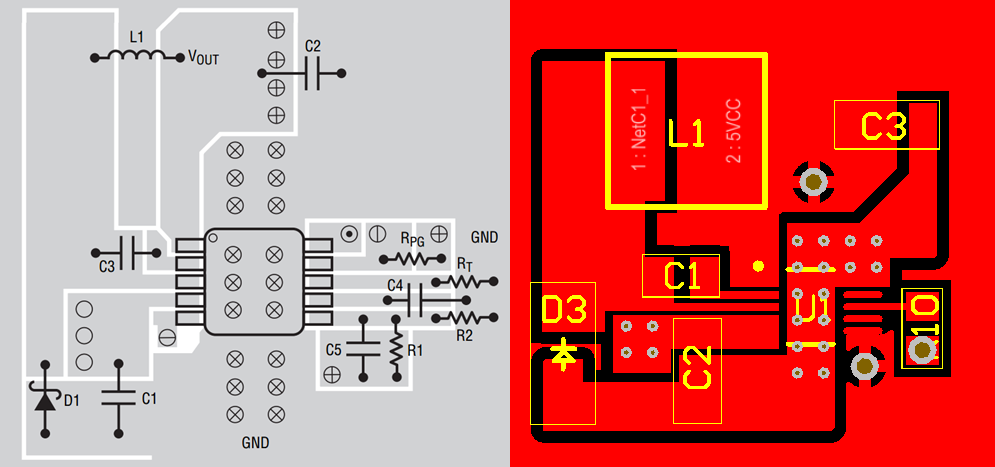
\includegraphics[width=0.8\textwidth]{Illustrationen/6-Umsetzung/LT3971_Layout.png}
	\caption{Layout LT3971: Datenblatt \protect\cite{LT3971_Datasheet}, Mainboard PCB}
	\label{fig:LT2971_Layout}
\end{figure}

\subsubsection{HMI Interface} \label{sec:Mainboard_HMI_Interface}
Das HMI bildet die Schnittstelle zwischen Operator und Planting Robot. Der Planting Robot soll so einfach wie möglich zu bedienen sein. Auf ein Touchscreen Interface oder Displays mit Menüführung durch Taster wird daher bewusst verzichtet. Stattdessen werden Taster mit blau, grün und weisser LED-Ring Beleuchtung (siehe Abb. \ref{fig:Taster_LED-Ring}) verwendet. Die Funktionen des Planting Robots werden dabei durch korrespondierende Taster realisiert. Die Funktionen des HMI werden in Kapitel \ref{sec:HMI} erklärt.
\begin{figure}[H]
	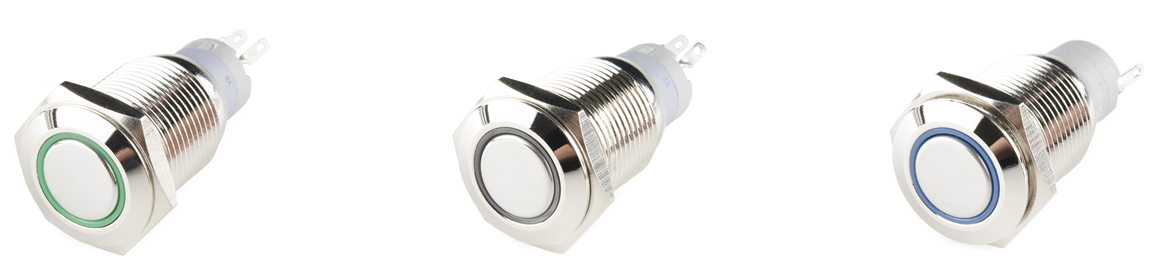
\includegraphics[width=0.9\textwidth]{Illustrationen/6-Umsetzung/HMI_LED_Taster.png}
	\caption{HMI Taster mit LED Ring \protect\cite{HMI_Taster}}
	\label{fig:Taster_LED-Ring}
\end{figure}

In Summe werden für das HMI 11 Taster und 14 LEDs angesteuert. Gemäss Tabelle \ref{tab:FRDM_Port_Mapping} sind zu wenig freie GPIO Ports Verfügbar um das HMI vollständig an Digital I/O Pins des FRDM-Boards anzuschliessen. Um die Anzahl benötigter GPIOs zu reduzieren könnten folgende Beschaltungen verwendet werden:
\begin{itemize}
	\item Tasterauswertung durch ADC
	\item Keyboard Matrix
	\item LED Treiber
\end{itemize}

\textbf{Tasterauswertung durch ADC:} Für diese Implementierungsvariante wird lediglich 1 Analog Input Pin benötigt. Dieser muss allerdings kontinuierlich ausgewertet werden und kann nicht über einen Interrupt gesteuert werden wie ein Digital Input.

\begin{figure}[H]
	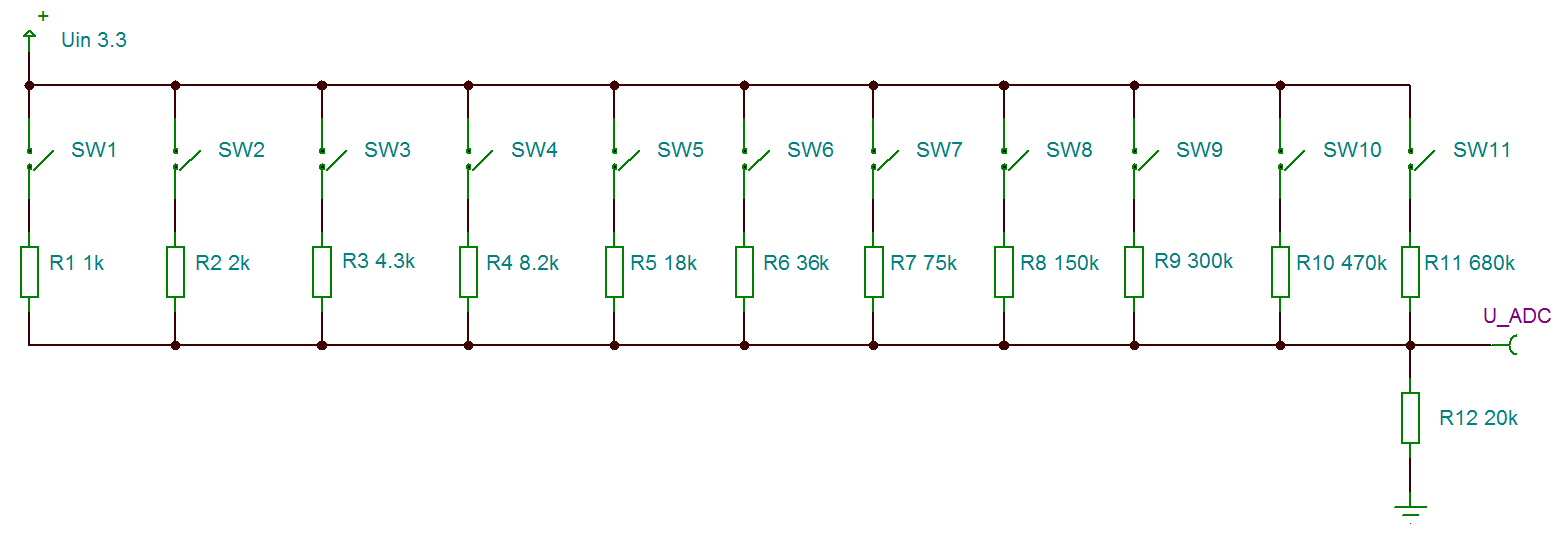
\includegraphics[width=1\textwidth]{Illustrationen/6-Umsetzung/Spannungsteiler_ADC.png}
	\caption{Tasterauswertung durch ADC}
	\label{fig:Spannungsteiler_ADC}
\end{figure}

Wenn davon ausgegangen werden kann, dass jeweils nur ein Taster zur gleichen Zeit gedrückt wird entstehen so 11 mögliche Spannungszustände am ADC Pin. Ein grosser Nachteil dieser Schaltung ist die grosse Komplexität der Spannungsauswertung wenn mehrere Taster gleichzeitig gedrückt werden. Beim Aufbau in Abb. \ref{fig:Spannungsteiler_ADC} mit 11 Tastern sind somit

\begin{equation}\label{nZustaende}
n_{Zustaende} = 2^{n_{Taster}} = 2^{11} = 2048
\end{equation}

Zustände auszuwerten. Bei einer linearen Skalierung dieser Zustände auf den ADC Spannungsbereich von 3.3V müsste folgende Spannungsdifferenz detektiert werden:

\begin{equation}\label{deltaU}
\bigtriangleup U = \frac{U_{in}}{n_{Zustaende}} = \frac{3.3V}{2048} = 1.61mV
\end{equation}

Solche geringen Spannungsdifferenzen für ein Taster Interface auszuwerten ist aufgrund des Aufwandes nicht sinnvoll, zumal eine lineare Aufteilung der Spannungspegel über den 3.3V Bereich mit Widerständen aus der Standard E12-Reihe nicht möglich ist. Die Anzahl Taster könnte auch auf mehrere ADC Eingänge des uC aufgeteilt werden, wodurch deutlich weniger verschieden Spannungspegel zu detektieren wären und diese sich im Wert stärker unterscheiden würden.\newline

\textbf{Keyboard Matrix:} Eine weit verbreitet Möglichkeit eine grosse Anzahl Taster auszuwerten ist eine Keyboard Matrix. Durch die Anordnung der Taster in Matrizenform kann die Anzahl benötigter GPIO Ports reduziert werden. Bei dieser Beschaltung wird jeweils Zeilenweise ein Low-Pegel auf die Matrize getrieben und dann Spaltenweise ausgelesen. Zur Veranschaulichung dient die folgende 4x4 Taster Matrize für ein Keypad in Abb. \ref{fig:Keyboard_Matrix}.

\begin{figure}[H]
	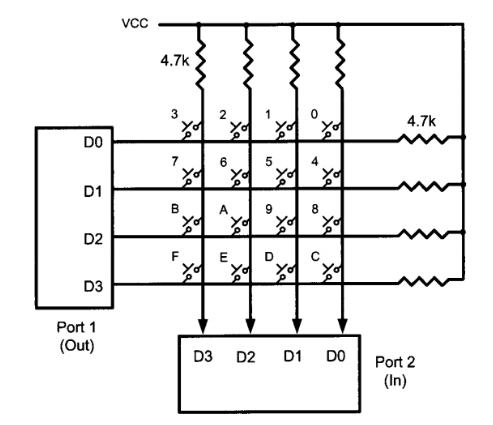
\includegraphics[width=0.4\textwidth]{Illustrationen/6-Umsetzung/Keyboard_Matrix.png}
	\caption{4x4 Keyboard Matrix \protect\cite{Keyboard_Matrix}}
	\label{fig:Keyboard_Matrix}
\end{figure}

Für die Auswertung von 11 Tastern müsste so eine 3x4 Matrize gebildet werden, welche demnach 7 GPIO Ports beanspruchen würde. Somit könnten lediglich 4 GPIO Ports am uC eingespart werden. Die Anzahl Anschlüsse kann mit einer Keyboard Matrix vor allem bei steigender Ordnung der Matrize drastisch reduziert werden. Für unsere Anwendung macht sie eher wenig Sinn, zumal die Softwareauswertung der GPIO Ports dadurch komplexer wird. Eine Keyboard Matrix kann auch über ein entsprechendes IC wie z.B. den LM8330 von TI ausgewertet werden. Dieses IC wird an den I$^2$C Bus angeschlossen und übernimmt die Matrizenauswertung inklusive entprellen der Taster. Der LM8330 ist allerdings nur im DSBGA Package (siehe Abb. \ref{fig:DSBGA_Package}), in der Grösse 2mm x 2mm, erhältlich. Dieses Package ist im Leiterplatten Prototypenbau nicht verwendbar, da es nicht von Hand bestückt werden kann.\newline

\begin{figure}[H]
	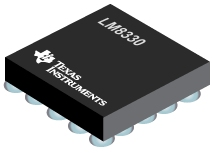
\includegraphics[width=0.3\textwidth]{Illustrationen/6-Umsetzung/DSBGA_Package.png}
	\caption{LM8330 DSBGA Package \protect\cite{DSBGA_Package}}
	\label{fig:DSBGA_Package}
\end{figure}

\textbf{LED Treiber:} Um GPIO Ports am uC einzusparen und um einen höheren Diodenstrom liefern zu können, wird der LP3943 LED Treiber Baustein von TI verwendet. Er verfügt über ein I$^{2}$C Schnittstelle für die Kommunikation zum FRDM-Board. Das genaue Kommunikationsprotokoll und dessen Verwendung werden im Kapitel \ref{} behandelt. Der LP3942 ist durch sein Open-Drain Treiberstufe in der Lage bis zu 25mA pro LED Pin und 200mA pro Package zu treiben. Das IC verfügt weiterhin über zwei Integrierte Timer, durch welche zwei PWM Signale zum dimmen der LEDs generiert werden können. Der Tastgrad des PWM Signals kann dabei von 0\%... 100\% in ein 1 Byte Register geschrieben werden. Die Timerfrequenz kann zwischen 0.625Hz und 160Hz gewählt werden. In Abb. \ref{fig:Mainboard_LED_Driver_LP3943} ist ein Auszug aus dem Schema des Mainboard PCBs illustriert. 

\begin{figure}[H]
	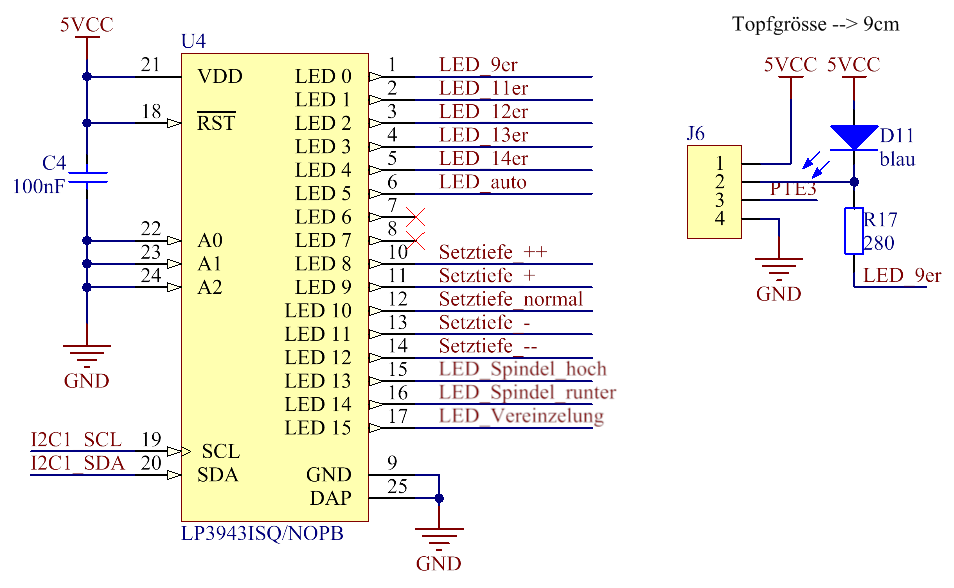
\includegraphics[width=0.7\textwidth]{Illustrationen/6-Umsetzung/Schema_Mainboard_LP39431.png}
	\caption{Schema Mainboard PCB, LED Treiber}
	\label{fig:Mainboard_LED_Driver_LP3943}
\end{figure}

Links ist der LED Treiber LP3943 zu sehen. Alle LEDs für das HMI sind daran angeschlossen. Über die Adressleitungen A0... A2 können die letzten 3 Bit der I$^{2}$C Adresse des Treibers bestimmt werden. In dieser Anwendung sind diese Digital Eingänge alle mit GND potential verbunden und somit auf logisch "0" konfiguriert. Auf der rechten Seite der Abbildung ist der Stecker J6 für einen Taster mit LED-Ring abgebildet. Alle HMI Taster mit LED-Ring werden jeweils über einen eigenen 4Pin Molex MicroFit Stecker verdrahtet (siehe Abb. \ref{fig:Mainboard_HMI_Layout}). Dabei wird der LED-Ring des Taster an Pin 1 und 2, der NO Kontakt an Pin 3 und der GND Kontakt an Pin 4 des Steckers angeschlossen.

\begin{figure}[H]
	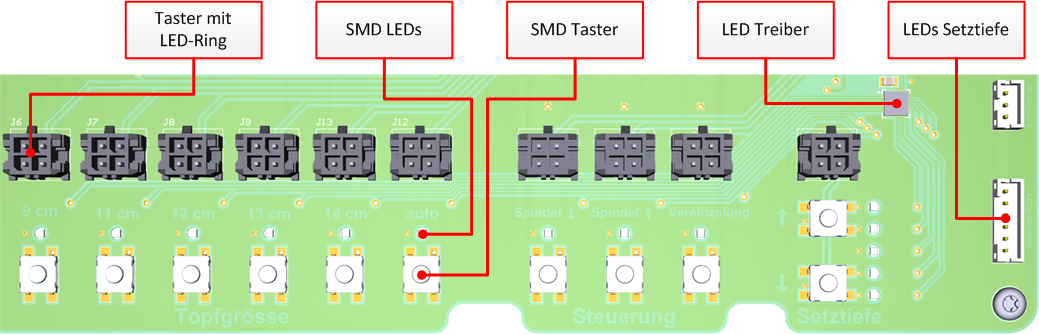
\includegraphics[width=1\textwidth]{Illustrationen/6-Umsetzung/HMI_Layout.png}
	\caption{Mainboard PCB, Onboard HMI}
	\label{fig:Mainboard_HMI_Layout}
\end{figure}

 Um die Software in Betrieb zu nehmen und zu testen, ohne das die Drucktaster verkabelt werden müssen, sind auf dem Mainboard bereits alle LEDs und Taster des HMI als SMD Bauteile bestückt. Alle LEDs auf dem Mainboard PCB sind $"$rear mounted$"$ LEDs. Diese werden auf dem Bottom Layer bestückt und leuchten durch eine Bohrung im PCB in Top Richtung. Durch diese Bauform bleibt mehr Platz auf dem Top Layer für Beschriftungen.





\subsection{Baseboard PCB}
\textit{(pro)}
Das Baseboard PCB dient als Sockel für den Motoren Controller TMCM-1630-2C von Trinamic. Trinamic bietet selbst ein Baseboard für diesen Controller an, dieses verfügt jedoch über eine RS232 EIA Schnittstelle und kann somit nicht direkt mit der UART Schnittstelle auf TTL Basis des FRDM-Board kommunizieren. Deshalb wurde im Umfang dieses Projekts ein eigenes Baseboard designt, welches über die notwendigen Schnittstellen verfügt um es direkt mit dem Mainboard PCB zu koppeln. Alle wichtigen Komponenten sind in Abb. \ref{fig:Baseboard_3D} mit Beschriftungen versehen.

\begin{figure}[H]
	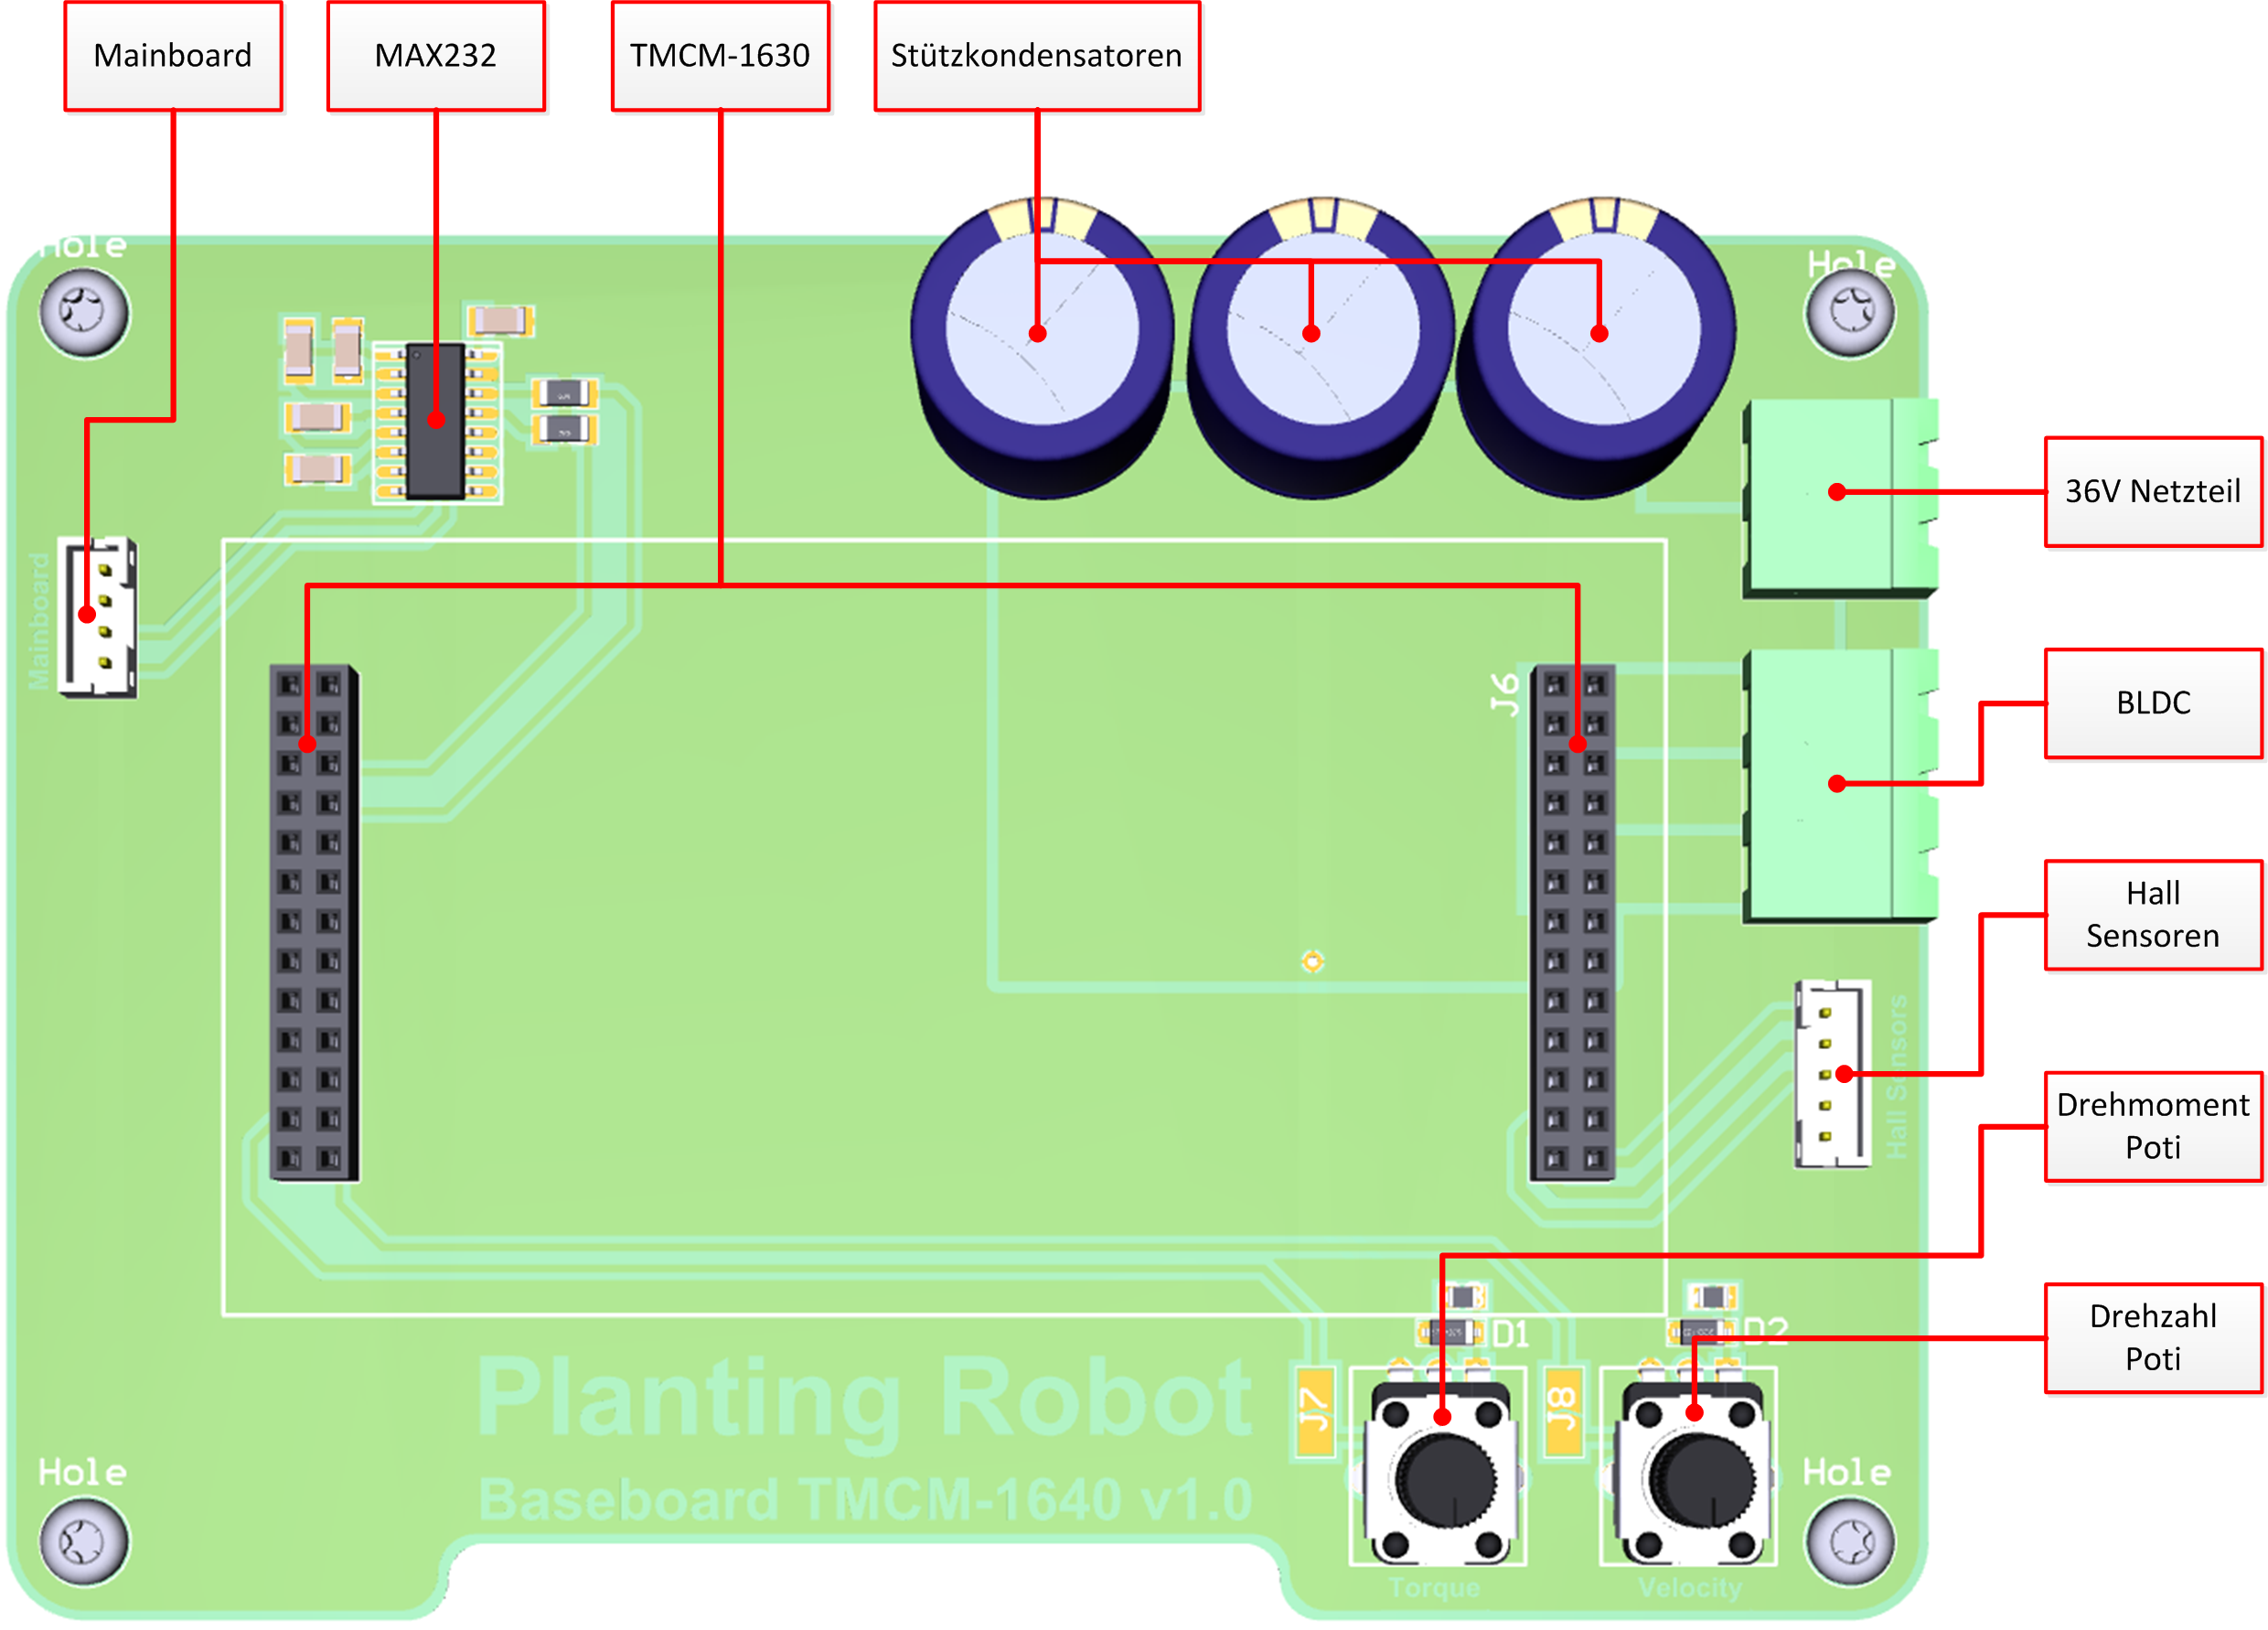
\includegraphics[width=1\textwidth]{Illustrationen/6-Umsetzung/Baseboard_3D_TOP.png}
	\caption{Baseboard PCB}
	\label{fig:Baseboard_3D}
\end{figure}

Die Verbindung zum Mainboard wir über einen 4 Poligen JST stecker realisiert. Auf ihn ist die UART Schnittstelle sowie das Signal Stop$\_$IN geführt. Das Stop $\_$IN Signal kann vom FRDM-Board auf GND gezogen werden um den Motorencontroller in den Not-Aus Modus zu bringen. Demnach wird der Motor gestoppt und der Controller muss durch ausschalten der Speisung zurückgesetzt werden. Der Schnittstellenwandler MAX232 von TI wandelt den UART TTL Pegel des FRDM-Board in den RS232 EIA Pegel des Motorencontrollers. Der Motorcontroller wird über zwei zweireihige Stiftleisten auf das Baseboard aufgesteckt. Dabei ist auf dem Motorencontroller TMCM-1630 \textbf{kein Verpolungsschutz} vorgesehen. Das Modul muss deshalb vor Inbetriebnahme zwingend wie folgt auf das Baseboard PCB gesteckt sein:

\begin{itemize}
	\item Der Bestückungsdruck des Motorcontrollers ist gleich ausgerichtet wie die Beschriftung $"$Planting Robot$"$ des Baseboard PCBs (nicht auf dem Kopf).
	\item Die LEDs des Motorcontrollers befinden sich auf der Seite des 4 Poligen JST Mainboard Steckers.
\end{itemize}

Um die Spannung auch bei hohen Laststromspitzen des BLDC Motors stabil zu halten werden drei 1mF Elektrolyt Kondensatoren Parallel zur Eingangsspannung geschaltet. Diese Vorgabe wurde dem Datenblatt des TMCM-1630 entnommen. Die 36V Eingangsspannung, sowie die Motorphasen werden über 90° Phoenix Stiftleisten der Serie MSTBA ausgeführt. Sie besitzen mit 10A den gleichen Nennstrom wie der Motorcontroller. Die Hall Sensoren des BLDC Motors werden über einen JST 5 Pol Stecker der Serie PH geführt. Für allfällige Testversuche während der Inbetriebnahme des BLDC Motors kann der Motorcontroller über die beiden Potentiometer im Standalone Modus betrieben werden. Die Analogsignale der beiden Potentiometer können über zwei lötbare Jumper vom Motorencontroller getrennt werden.
\subsection{Software} \label{sec:Software}
\textit{(pro)} Die Software des Planting Robots ist in der Programmiersprache C geschrieben und läuft auf dem ARM Cortex M0+ Mikrocontroller von NXP welcher auf dem FRDM-Board KL25Z bestückt ist. Für low Level Driver werden diverse Processor Expert Komponenten verwendet. Als Betriebssystem dient das Real Time OS FreeRTOS. Vorteile von FreeRTOS gegenüber anderen C Betriebssystemen sind:

\begin{itemize}
	\item Seine geringen Ressourcenanforderungen an RAM, ROM und CPU Leistung. 
	\item FreeRTOS ist weit verbreitet und wird an der HSLU in diversen Softwareprojekten verwendet.
	\item Es ist absolut kostenfrei, auch für kommerzielle Anwendungen.
	\item FreeRTOS ist einfach in der Anwendung, eignet sich jedoch auch für grössere Projekte.
\end{itemize}

In den folgenden Unterkapiteln werden die wichtigsten Softwarekomponenten des Planting Robots beschrieben und erklärt. Die Titel der Unterkapitel korrespondieren dabei mit den Namen der .c Files des Codes im Anhang.

\subsubsection{FSM} \label{sec:FSM}
Der Planting Robot wird durch einen endlichen Zustandsautomaten FSM gesteuert. Die Zustände oder States die FSM sind in Abb. \ref{fig:FSM} illustriert. Ein State Wechsel wird entweder durch eine User Eingabe übe das HMI, eine Topferkennung durch den IR-Sensor oder durch fertigstellen eines States ausgeführt. Im folgenden Abschnitt werden die verschiedenen States sowie State-Wechsel erklärt:

\begin{figure}[H]
	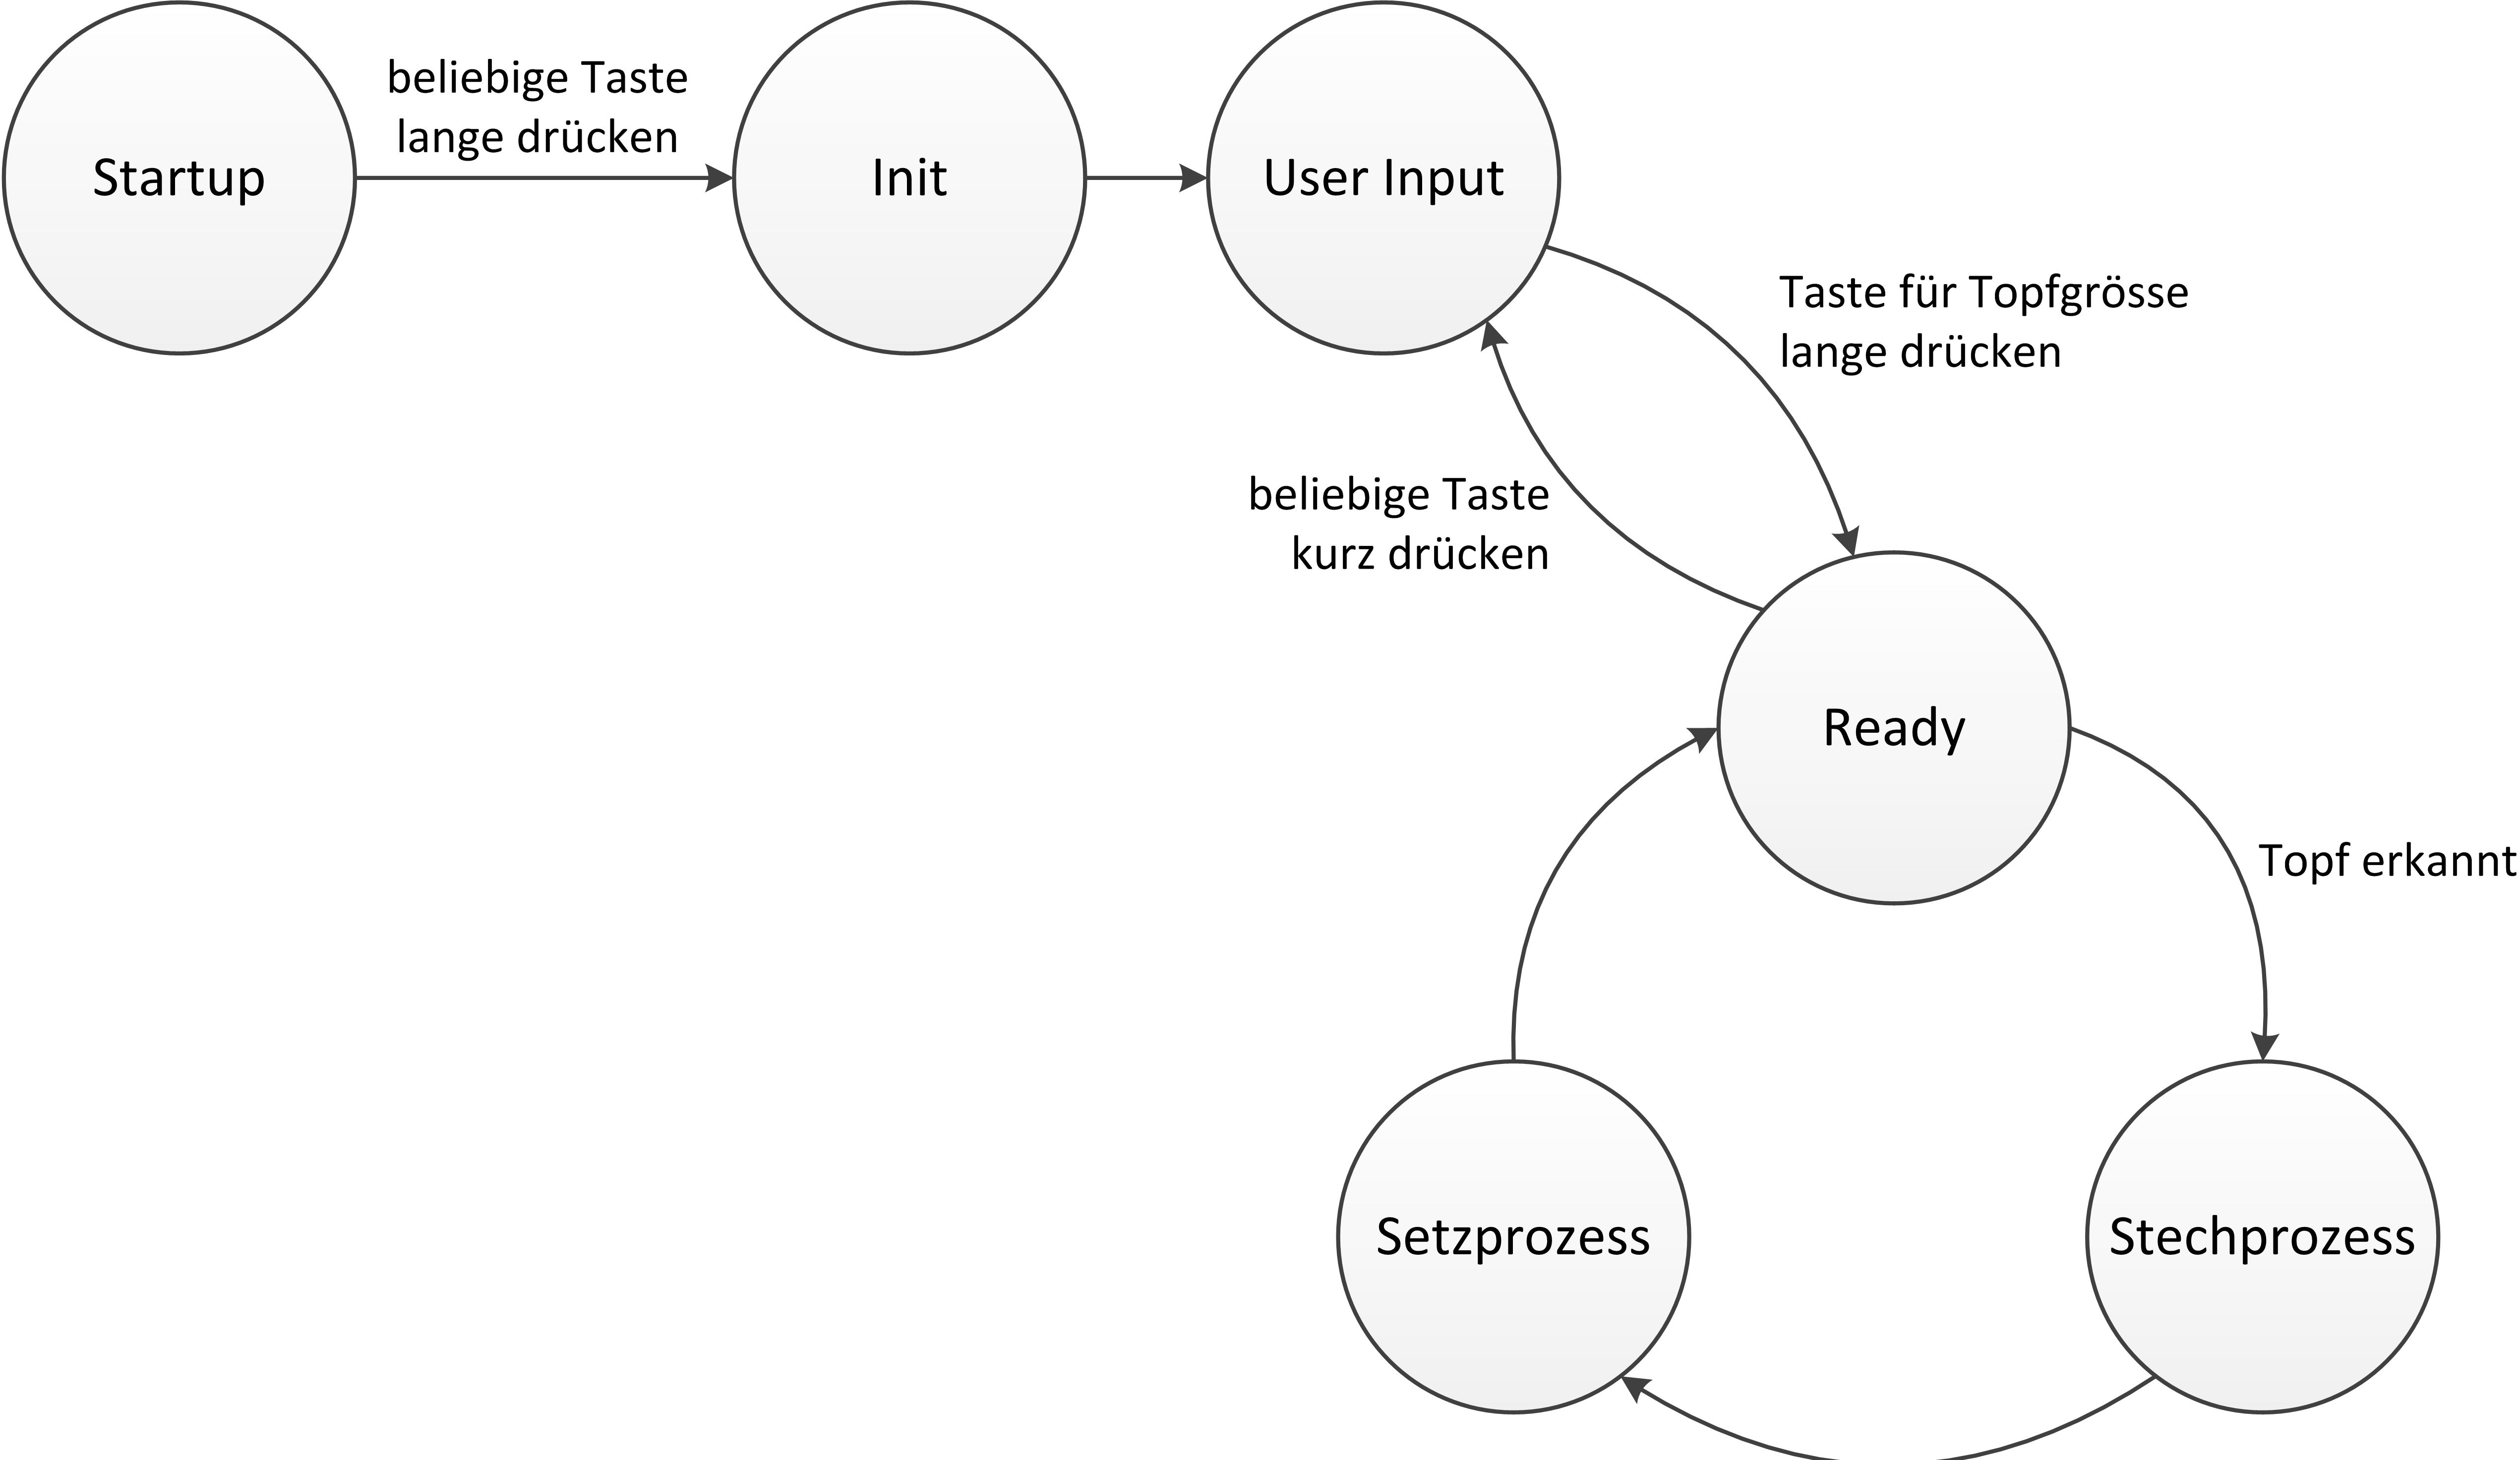
\includegraphics[width=0.9\textwidth]{Illustrationen/6-Umsetzung/FSM_B&W_breit.png}
	\caption{Software, FSM}
	\label{fig:FSM}
\end{figure}

\textbf{Startup:} Wenn die Speisung zum uC eingeschaltet wird, begibt sich die Software in den sicheren Zustand $"$Startup$"$. In diesem State sind sämtliche Aktoren stromlos. Alle LEDs des HMIs pulsieren synchron. Wird ein beliebiger Taster des HMIs länger als eine halbe Sekunde gedrückt wechselt die Software in den $"$Init$"$ State.\\
\newline
\textbf{Init:} In diesem State werden die Motoren für die Vereinzelung, die Verstellmechanik und die Setzeinheit initialisiert. Da die Motoren über Drehencoder und nicht über absolute Positionsencoder verfügen, müssen diese zuerst in ihre Ausgangsposition gebracht werden. Der Initialisierungsprozess zu den jeweiligen Motoren wird in den Kapiteln \ref{sec:Vereinzelung}, \ref{sec:Setzeinheit} und \ref{verstellmechanik} erklärt. Während der Initialisierung blinken die HMI LEDs des jeweiligen Prozesses. Nach Abschluss der Initialisierung wechselt die State Machine in den $"$User Input$"$ State.\\
\newline
\textbf{User Input:} Dieser State dient zur Konfiguration des Planting Robots. Der Operator kann hier die Topfgrösse des aktuellen Batches und die Setztiefe der Nemacaps über das HMI einstellen. Ausserdem kann der Planting Robot in diesem State manuell über die Tasten $"$manuelle Steuerung$"$ bedient werden. Mehr zur manuellen Steuerung ist im Kapitel \ref{sec:HMI} nachzulesen. Um die Konfiguration zu speichern und den Planting Robot in Betrieb zu setzen muss der Taster für die gewünschte Topfgrösse lange gedrückt werden.\\
\newline
\textbf{Ready:} Der Planting Robot befindet sich im regulären Betriebsmodus. Sobald ein Topf erkannt wird, verrichtet der Planting Robot seine Arbeit indem er den Stechprozess und anschliessend den Setzprozess ausführt. Um den Planting Robot zu stoppen, kann ein beliebiger Taster gedrückt werden. Der Planting Robot wechselt dann zurück in den $"$User Input$"$ State.\\
\newline
\textbf{Stechprozess:} Dieser Prozess wird durchlaufen sobald ein Topf erkannt wurde. Dabei wird mit dem Spindelantrieb eine Hubbewegung ausgeführt bei welcher der Stechdorn in die Erde gedrückt und wieder angehoben wird.\\
\newline
\textbf{Setzprozess:} Sobald der Stechprozess beendet ist wird der Setzprozess ausgeführt. Dabei wird die Vereinzlung angetrieben, sodass NemaCaps vom Schüttgutlager in die Topferde befördert wird. Nach beenden des Setzprozesses geht die FSM wieder in den $"$Ready$"$ State.

\subsubsection{HMI Driver}
Im HMI\_Driver.c File wird der HMI\_Task erzeugt. Alle 10ms führt dieser den Debounce Prozess aus. Dabei wird die Funktion FunktionKEYDBNC\_Process() aufgerufen, welche den Status aller Taster des HMIs ausliest und über eine State Machine entprellt. Der Debounce Prozess generiert dann ein Event für jeden Tastendruck, langen Tastendruck und loslassen eines Tasters. Events werden vom Event.c File in einem Event Array abgespeichert. Es wird somit ein Polling der HMI Taster mit einer Frequenz von 100Hz durchgeführt. Diese Programmsequenz ist in Abb. \ref{fig:Taster_Polling} oben grafisch dargestellt.


\begin{figure}[H]
	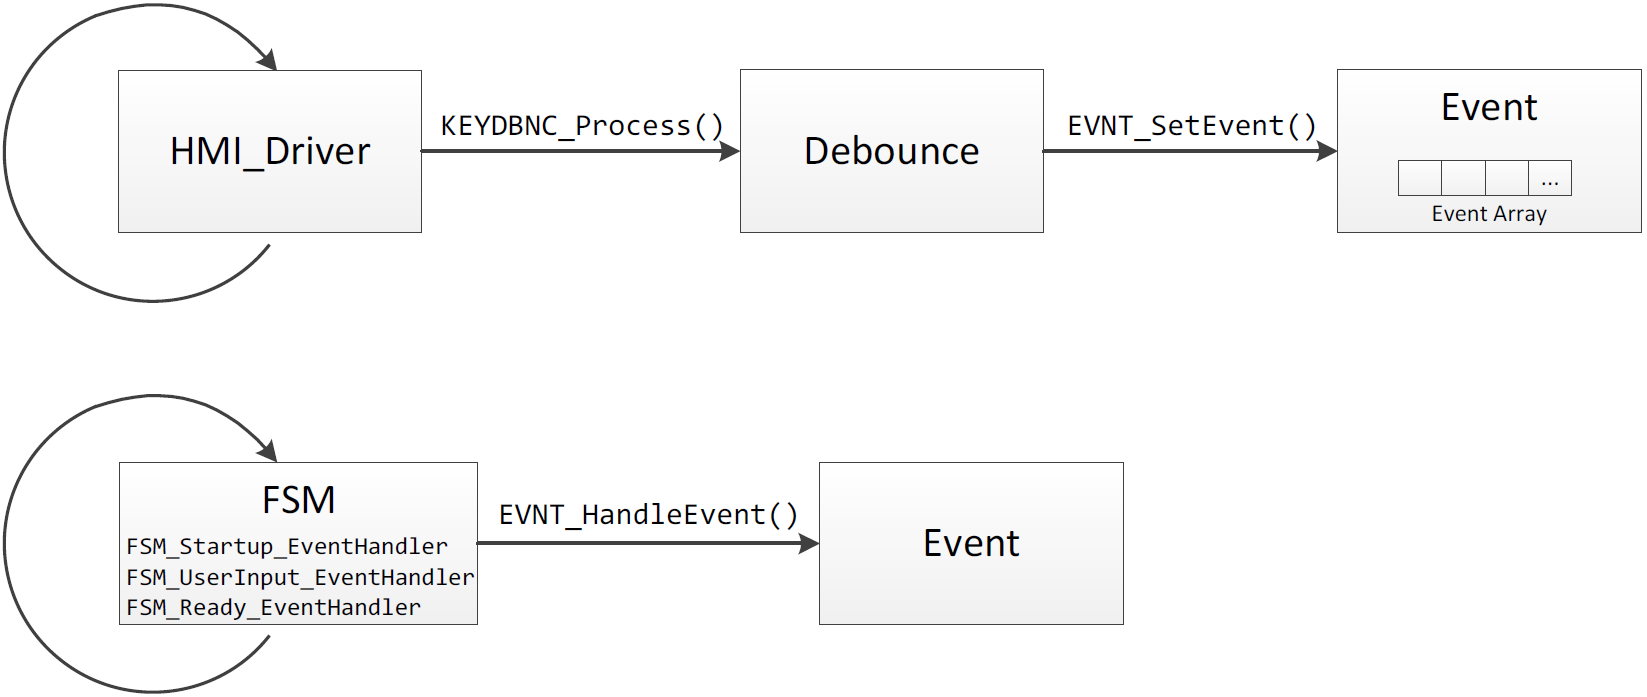
\includegraphics[width=0.9\textwidth]{Illustrationen/6-Umsetzung/Taster_Polling.png}
	\caption{Software, Taster Polling / Auswertung}
	\label{fig:Taster_Polling}
\end{figure}

Der untere Teil der Grafik in Abb. \ref{fig:Taster_Polling} beschreibt die Auswertung eines Tastendrucks. Dazu werden die vom Debounce Prozess erzeugte Events in einem der drei Eventhandler (FSM\_Startup\_EventHandler, FSM\_UserInput\_EventHandler oder FSM\_Ready\_EventHandler) des FSM.c Files ausgewertet. Eine solche Taster Event Auswertung ist am Beispiel des FSM\_Startup\_EventHandler im folgenden Code dargestellt:

\begin{lstlisting}
void FSM_Startup_EventHandler(EVNT_Handle event) {
	switch(event) {
		case EVNT_BTN_9cm_LPRESSED:				// Any Button Long Press
		case EVNT_BTN_11cm_LPRESSED:
		case EVNT_BTN_12cm_LPRESSED:
		case EVNT_BTN_13cm_LPRESSED:
		case EVNT_BTN_14cm_LPRESSED:
		case EVNT_BTN_AUTO_LPRESSED:
		case EVNT_BTN_Setzeinheit_runter_LPRESSED:
		case EVNT_BTN_Setzeinheit_hoch_LPRESSED:
		case EVNT_BTN_Vereinzelung_LPRESSED:
		case EVNT_BTN_hoeher_LPRESSED:
		case EVNT_BTN_tiefer_LPRESSED:
			LED_Driver_pulseAll(FALSE);
			LED_Driver_clear_all();
			fsmData.fsmState = Init;
			break;
		default:
			break;
	} /* switch */
}
\end{lstlisting}

Der Code beschreibt das Verhalten des Planting Robots auf einen Tastendruck während des Startup States wie in Kapitel \ref{sec:FSM} beschrieben. \\
\newline
Die .c Files Debounce, Event, KeyDebounce und Trigger beruhen Grundlegend auf den Gleichnamigen Files aus dem Modulunterricht INTRO, betreut durch Erich Styger. Der Code wurde jedoch für die Verwendung mit dem Planting Robot angepasst und erweitert.

\subsubsection{LED Driver}
Wie in Kapitel \ref{sec:Mainboard_HMI_Interface} erklärt, wird für die Ansteuerung der HMI LEDs der LED Treiber Baustein LP3943, mit I$^{2}$C Schnittstelle verwendet. Die I$^{2}$C Schnittstellenparameter wurden gemäss Tabelle \ref{tab:I2C_Parameter} in Processor Expert konfiguriert:

\begin{table}[H]
	\centering
	\caption{Software, I$^{2}$C Parameter LED Treiber}
	\begin{tabular}{|l|c|r|}
		\hline
		\textbf{Parameter} & \textbf{Wert} & \textbf{Einheit} \\
		\hline
		SCL frequency & 109.227 & kHz \\
		\hline
		SDA Hold & 0.811 & us \\
		\hline
		SCL start Hold & 4.482 & us \\
		\hline
		SCL stop Hold & 4.625 & us \\
		\hline
		Adress mode & 7     & bit \\
		\hline
	\end{tabular}%
	\label{tab:I2C_Parameter}%
\end{table}%

In Tabelle \ref{tab:LP3943_Register} sind sämtliche Funktions Register des LP3943 aufgelistet. Die LEDs des HMI können durch schreiben der Register LS0... LS3 konfiguriert werden. Dabei kann jeder LED Port einen der folgenden vier Konfigurationen annehmen: LED aus, LED ein, LED dimmen mit Dimmrate DIM0, LED dimmen mit Dimmrate DIM1. Die Dimmraten DIM0 und DIM1 sind durch Timer Bausteine definiert. Demnach kann für jeden der beiden Timer über die Register Prescaler und PWM eine Frequenz und ein Tastgrad konfiguriert werden. Da über das Prescaler Register eine Periodenzeit von 6.25ms... 1.6s eingestellt werden kann, können die LEDs gut sichtbar zum blinken gebracht werden.

\begin{table}[H]
	\centering
	\caption{LP3943 Register Tabelle \protect\cite{LP3943}}
	\begin{tabular}{|l|l|l|l|}
		\hline
		\textbf{Adress (Hex)} & \textbf{Register Name} & \textbf{Read/Write} & \textbf{Register Function} \\
		\hline
		0x00  & Input 1 & Read only & LED0–7 Input Register \\
		\hline
		0x01  & Input 2 & Read only & LED8–15 Input Register \\
		\hline
		0x02  & PSC0  & R/W   & Frequency Prescaler 0 \\
		\hline
		0x03  & PWM0  & R/W   & PWM Register 0 \\
		\hline
		0x04  & PSC1  & R/W   & Frequency Prescaler 1 \\
		\hline
		0x05  & PWM1  & R/W   & PWM Register 1 \\
		\hline
		0x06  & LS0   & R/W   & LED0–3 Selector \\
		\hline
		0x07  & LS1   & R/W   & LED4–7 Selector \\
		\hline
		0x08  & LS2   & R/W   & LED8–11 Selector \\
		\hline
		0x09  & LS3   & R/W   & LED12–15 Selector \\
		\hline
	\end{tabular}%
	\label{tab:LP3943_Register}%
\end{table}%

Durch Verwendung der Register Input 1 sowie Input 2 können die Pins des LP3943 auch als Digital Inputs verwendet werden. In diesem Projekt wird der LP3943 allerdings nur zum treiben von LEDs verwendet.

\subsubsection{ION Motion Driver}
Der ION Motion Motorcontroller wird über UART mit einer Baudrate von 38400 baud angesteuert. Das Interface des Motorencontrollers besteht aus über 50 Befehle und ist nicht sehr übersichtlich. In Tabelle \ref{tab:ION_Kommandos} sind die in diesem Projekt verwendeten Kommandos zusammen mit der Menge Datenbytes aufgelistet. Dabei ist die Menge an Datenbytes, bei Kommandos welche mehrere Parameter übergeben, die Summe der jeweiligen Ziffern. So werden für das Kommando Nr. 65 beispielsweise 16 Datenbytes gesendet.

\begin{table}[H]
	\footnotesize
	\centering
	\caption{Software, ION Motion Kommandos}
	\begin{tabular}{|c|l|c|}
		\hline
		\multicolumn{1}{|l|}{\textcolor[rgb]{ .247,  .247,  .247}{\textbf{Kommando}}} & \textcolor[rgb]{ .247,  .247,  .247}{\textbf{Beschreibung}} & \multicolumn{1}{l|}{\textcolor[rgb]{ .247,  .247,  .247}{\textbf{Datenbytes}}} \\
		\hline
		0     & Drive Forward Motor 1 & 1 \\
		\hline
		1     & Drive Backwards Motor 1 & 1 \\
		\hline
		4     & Drive Forward M2 & 1 \\
		\hline
		5     & Drive Backwards M2 & 1 \\
		\hline
		22    & Set Quadrature Encoder 1 Value & 4 \\
		\hline
		23    & Set Quadrature Encoder 2 Value & 4 \\
		\hline
		49    & Read Motor Currents & 2 / 2 \\
		\hline
		65    & Buffered Drive M1 with signed Speed, Accel, Deccel and Position & 4 / 4  / 4 / 4 \\
		\hline
		66    & Buffered Drive M2 with signed Speed, Accel, Deccel and Position & 4 / 4  / 4 / 4 \\
		\hline
	\end{tabular}%
	\label{tab:ION_Kommandos}%
\end{table}%

Kommandos werden gemäss folgendem Schema gesendet: Address Byte, Command Byte, Data Bytes, CRC 16Bit checksum.  Nach dem empfangen eines gültigen Kommandos antwortet der Kontroller mit einem acknowledge Byte (0xFF) oder direkt mit den geforderten Datenbytes gefolgt von der 16Bit checksum.\\ 
Aufgrund der unterschiedlichen Menge an Datenbytes ist es schwierig eine generische Methode für alle Kommandos zu schreiben. Diese würde schnell sehr gross und unübersichtlich. Deshalb werden die Kommandos aus Tab. \ref{tab:ION_Kommandos} in einer der vier Methoden setMotorSpeed, setEncoderValue, getMotorCurrent und ION\_Motion\_setPosition behandelt. Die Aufteilung der Kommandos auf die jeweiligen Methoden ist in Abb. \ref{fig:ION_Methoden} abgebildet.

\begin{figure}[H]
	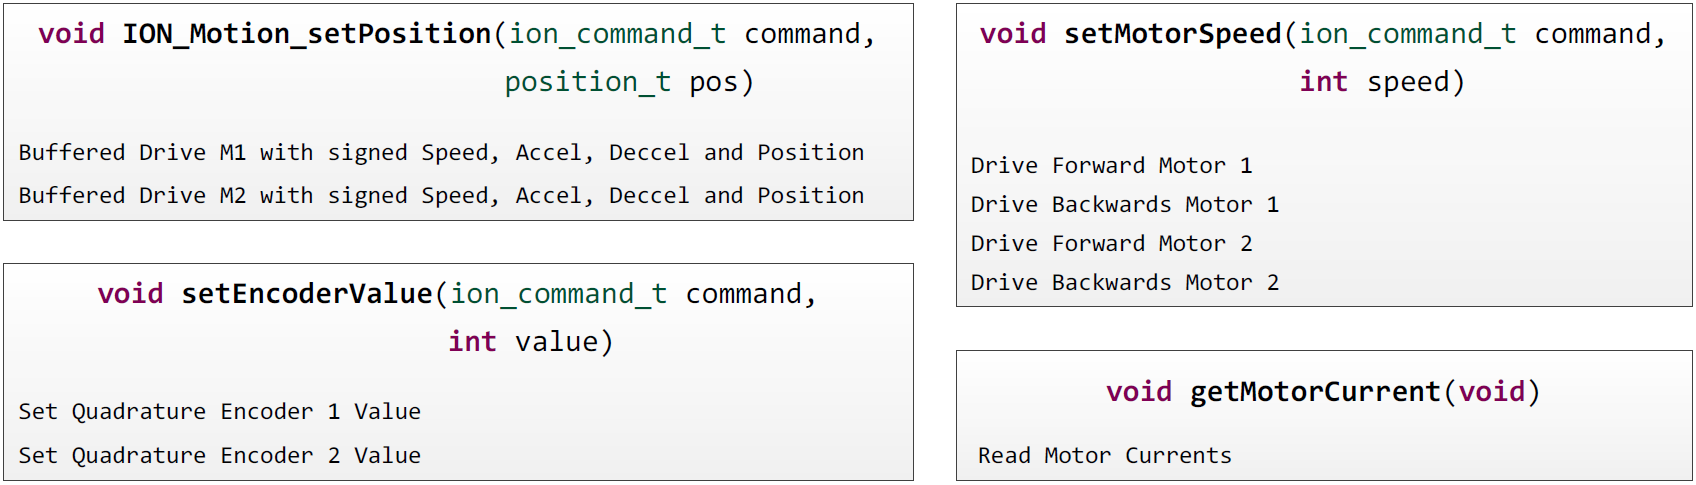
\includegraphics[width=1\textwidth]{Illustrationen/6-Umsetzung/ION_Funktionen.png}
	\caption{Software, ION Motion Driver Methoden}
	\label{fig:ION_Methoden}
\end{figure}

Auf Basis dieser vier Methoden wurde die Ansteuerung der Motoren für die Vereinzelung und die Verstellmechanik implementiert. Die beiden Prozesse sind in den Kapiteln Vereinzelung (\ref{sec:Vereinzelung}) und Verstellmechanik (\ref{verstellmechanik}) systematisch beschrieben. Die genaue Implementierung der vier Methoden kann im ION\_Motion\_Driver.c File im Anhang nachgeschlagen werden. Im folgenden Absatz wird noch kurz auf die Auswertung der mit dem Motorcontroller gemessen Motorstromwerte eingegangen.\newline
Für die Initialisierung der Verstellmechanik wird der Motor langsam in eine Richtung gedreht bis die Welle an den mechanischen Anschlag läuft. In diesem Moment steigt der Strom durch den Motor aufgrund der erhöhten Last stark an. Dieser Anstieg wird über die Auswertung der Stromwerte detektiert. Im konkreten Fall wird in der Software ein Schwellwert für die Stromstärke definiert, bei welchem der Motor angehalten soll. Um die Fluktuationen der gemessenen Stromwerte zu glätten wird ein Mittelwert über die letzten X Werte gebildet.


\begin{figure}[H]
	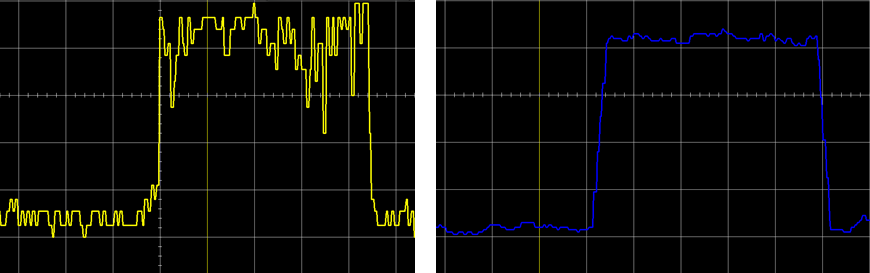
\includegraphics[width=1\textwidth]{Illustrationen/6-Umsetzung/ION_Motion_Strommessung.png}
	\caption{Software, Glättung des Motorstroms}
	\label{fig:ION_Motion_Strommessung}
\end{figure}

In Abbildung \ref{fig:ION_Motion_Strommessung} ist der Stromverlauf des Pololu Getriebemotors mit Übersetzung 378:1 abgebildet. Die Messung wurden mit der Software Segger J-Scope durchgeführt. Der Motor wurde im Leerlauf ohne Last betrieben, mit einer konstanten Last gebremst und anschliessend wieder entlastet. Dabei wurde der Motor mit einem geringen PWM Tastgrad betrieben um keinen zu grossen Laststrom zu generieren.\\
Auf den beiden Graphen ist ein deutlicher Stromanstieg zu erkennen. Der linke Graph zeigt dabei die gemessenen Stromwerte, der rechte die Mittelwerte der letzten 5 Messwerte. Der Vorteil der Mittelwertbildung kommt vor allem bei einer konstanten Belastung des Motors zum Vorschein, da hier die gemessenen Stromwerte stark fluktuieren und keine akkurate Messung zulassen. Die Stromkurven sind als qualitative Angaben zu verstehen, der Fokus liegt auf der Glättung der Messwerte.


\subsubsection{IR Sensor Driver}
Dieser Teil der Software befasst sich mit der Messgrössenerfassung und Auswertung der IR-Sensor Daten zur Topferkennung. Dabei setzt sich die Topferkennung gemäss folgender Aufzählung aus zwei Teilen zusammen:

\begin{itemize}
	\item Die Erkennung eines Topfes welcher sich vor dem Planting Robot in Position befindet um mit Nemacaps besetzt zu werden.
	\item Das Erkennen von verschiedenen Topfgrössen zur Laufzeit der Anlage. Dadurch soll sich die Verstellmechanik adaptiv an einen neuen Produktionsbatch mit anderen Töpfen anpassen.
\end{itemize}

Die Softwareauswertung der Topferkennung wurde aus Zeitgründen nicht mehr implementiert. Allerdings wurde ein Prove of Concept der Messmethode zur Erkennung der Topfposition durchgeführt. Dieses ist in Kapitel \ref{sec:Topferkennung} beschrieben.

\subsubsection{Trinamic Motion Driver}


\subsection{Topferkennung} \label{sec:Topferkennung}
\textit{(pro)} Als Sensor für die Topferkennung wurde der IR Distanzsensor von Sharp mit der Typenbezeichnung GP2Y0A41SK0F evaluiert. Er verfügt über einen Messbereich von 40mm... 300mm und ermittelt die Distanz durch Triangulation. Das Messsignal wird als Analog Pegel von 0V... 3.1V dargestellt.\\
Die Softwareauswertung der Topferkennung wurde aus Zeitgründen nicht mehr implementiert. Allerdings wurde ein Prove of Concept der Messmethode durchgeführt. Dieses wird in Kapitel \ref{sec:Topferkennung_ProveOfConcept} erklärt.



\subsubsection{Topfposition}
Die Informationen der Testmessung wurden als ausreichend empfunden um damit die Bewegungsphase eines Topfes zu erkennen und dementsprechend den Setzprozess auszulösen. Dafür wird der Sensor so platziert, dass sich der Topf im Stillstand direkt vor dem Sensor befindet. Durch die Stopp and Go Bewegung des Topfkranzes der Topfmaschine TC5 entsteht ein Signalbild wie in Abb. \ref{fig:Signalbild_Topferkennung} illustriert.\\

\begin{figure}[H]
	\includegraphics[width=0.9\textwidth]{Illustrationen/6-Umsetzung/Topferkennung_Messsignal.png}
	\caption{Topferkennung, Signalverlauf Topferkennung}
	\label{fig:Signalbild_Topferkennung}
\end{figure}

Um nun die Eingriffszeit T$_{e}$ bestimmen zu können, werden die Messwerte miteinander verglichen. Wenn die Messwerte in einem bestimmten Pegelbereich konstant bleiben kann davon ausgegangen werden, dass der Topf still steht.

\subsubsection{Topfgrösse}
Für die Messung der Topfgrösse reicht ein Sensor allerdings nur bedingt aus, da er aufgrund von überstehender Pflanzenerde eine Fehlmessung verursachen könnte. Um mit einer Distanzmessung zum Topf eine präzise Aussage über die Grösse des Topfes zu treffen, müsste zusätzlich die Geschwindigkeit des Topfkranzes erfasst werden. Eine weitere Möglichkeit wäre die Topfgrössenerkennung  durch Einsatz eines Echtzeit Bildverarbeitungssystems. Diese Sachverhalte führen zur Erkenntnis, dass die Topfgrössenerkennung einen zu grossen zeitlichen Aufwand für dieses Projekt bedeuten würde. Deshalb wird die Wunschanforderung nach einer automatischen Topfgrössenerkennung im Umfang dieses Projekts nicht realisiert.

\subsection{HMI} \label{sec:HMI}
In diesem Kapitel wird der Aufbau und die Funktionen des HMI erklärt. Das Kapitel behandelt die HMI Maske, die entwickelte Leiterplatte und eine Bedienungsanleitung für den Umgang mit dem Planting Robot.

\subsubsection{Aufbau}
Alle Bedieneinheiten des HMI sollten dem Operator einfach zugänglich auf einem Blech platziert sein. Um die Übersicht über die 11 Taster und 14 LEDs zu behalten wurde die HMI Maske (siehe Abb. \ref{fig:HMI_Maske}) gezeichnet. Die Maske wurde dabei auf eine transparente Folie aufgedruckt und auf das Aluminium Blech aufgeklebt.

\begin{figure}[H]
	\includegraphics[draft=false,width=0.85\textwidth]{Illustrationen/6-Umsetzung/HMI_Foto.jpg}
	\caption{HMI Blech und Maske}
	\label{fig:HMI_Maske}
\end{figure}

Nebst den LEDs in den Drucktastern verfügt das HMI über 5 LEDs für die Anzeige der einstellbaren Setztiefe der NemaCaps. Diese LEDs sind auf dem HMI LED PCB bestückt und über light pipes durch das HMI Blech geführt. Light pipes ermöglichen das bündeln und führen von Licht. In dieser Anwendung werden sie verwendet um die LED Anzeige ästhetisch ansprechend auf dem HMI Blech zu integrieren.

\begin{figure}[H]
	\includegraphics[draft=false,width=0.8\textwidth]{Illustrationen/6-Umsetzung/LED_PCB_3D.jpg}
	\caption{HMI LED PCB}
	\label{fig:LED_PCB_1}
\end{figure}

\subsubsection{Bedienungsanleitung}
Im folgenden Abschnitt wird die Bedienung des Planting Robots Schritt für Schritt erklärt. Achtung! Der Planting Robot ist ein Prototyp. Demnach kann es bei unsachgemässer Bedienung potenziell zu Fehlfunktionen kommen. Als grafische Hilfestellung zur Bedienungsanleitung dient eine State Übersicht der Software in Abb. \ref{fig:Bedienungsanleitung}.

\begin{figure}[H]
	\includegraphics[draft=false,width=1\textwidth]{Illustrationen/6-Umsetzung/Bedienungsanleitung.png}
	\caption{Bedienungsanleitung, State Übersicht}
	\label{fig:Bedienungsanleitung}
\end{figure}

\begin{enumerate}
	\item Um den Planting Robot in Betrieb zu nehmen, muss der Einschalttaster auf der Rückseite des Maschinengestells gedrückt werden. Vergewissern Sie sich dabei, dass der Netzstecker eingesteckt und der Leitungsschutzschalter durchgeschaltet ist.
	\item Sofort nach drücken des Einschalttasters fangen die LEDs des HMIs an zu pulsieren. Der Planting Robot befindet sich im Startup State. In diesem State führt der Planting Robot keine seiner Funktionen aus. Durch einen langen Tastendruck (>0.5s) eines beliebigen Tasters, fängt der Planting Robot an seine Komponenten zu initialisieren. Dies wird durch das blinken der HMI Taster der entsprechenden Funktionen angezeigt. Die Initialphase dauert ca. 5... 10s.
	\item Nach Abschluss der Initialphase befindet sich die Software im User Input State. \textbf{Zu diesem Zeitpunkt muss sich die Setzeinheit an der obersten Ausgangsstellung befinden.} Ist dies nicht der Fall, muss der Planting Robot neu gestartet und die vorherigen Schritte wiederholt werden. Im User Input State können Einstellungen zu den Topfgrössen und der Setztiefe vorgenommen werden. Diese Funktionen werden im Unterkapitel $"$User Input$"$ erklärt. Durch langes drücken einer Topfgrössen Taste wird der Planting Robot in Betrieb gebracht.
	\item Die Software wechselt in den Ready State. Da die Topferkennung aus Zeitgründen nicht mehr implementiert wurde, führt der Planting Robot in diesem State ein Demo Programm aus und nicht wie in Kapitel \ref{sec:FSM} beschrieben den regulären Betriebsmodus. Das Demo Programm dient zu Vorführzwecken und kann durch einen beliebigen Tastendruck unterbrochen werden. Durch den Tastendruck wechselt die Software wieder zurück in den User $"$Input State$"$.
\end{enumerate}

\textbf{User Input}\\
Im $"$User Input$"$ State kann die Topfgrösse sowie die Setztiefe der Nemacaps konfiguriert werden. Um eine andere Topfgrösse einzustellen, muss auf dem HMI die entsprechende Grösse angewählt werden. Die Verstellmechanik führt den Befahl bei Tastendruck sofort aus und konfiguriert den Setzradius neu. Die Setztiefe wird auf dem HMI über 5 LEDs angezeigt. Dabei ist standardmässig die mittlere grüne LED aktiviert. Diese signalisiert eine mittlere Setztiefe. Durch drücken der beiden Taster rechts der LEDs kann die Setztiefe höher oder tiefer eingestellt werden. Diese Funktion ist in der Software der Setzeinheit noch nicht implementiert, die LEDs lassen sich zu Vorschauzwecken allerdings schon einstellen.\\
Eine weitere Funktion des $"$User Input$"$ States ist die manuelle Steuerung des Planting Robots. Über die Taster $"$Spindel hoch$"$ und $"$Spindel runter$"$ kann die Setzteinheit manuell hoch und runter bewegt werden. Die Taster müssen dafür länger als 0.5s gedrückt werden. Bei loslassen der Taster hält die Spindel wieder an. Durch Druck auf den Taster $"$Vereinzelung$"$ wird die Lochmaske der Vereinzelung um eine Position gedreht.
\subsection{Peripherie}

\subsubsection{Maschinengestell}
\label{maschinengestell}
\begin{wrapfigure}[16]{r}{6cm}
	\includegraphics[scale=0.41]{Illustrationen/6-Umsetzung/maschinengestell.PNG}
	\caption{Maschinengestell}
	\label{fig:maschinengestell}
\end{wrapfigure}

\textit{(ygu)} Das Maschinengestell basiert auf dem Baukasten System von Kanya AG. Die Profile von Kanya AG eignen sich aus folgenden Gründen:
\begin{itemize}
	\item Dieses System ist einfach im Aufbau und der Montage. Das Maschinengestell ist so aufgebaut, dass eine Anpassung der Höhe (Punkt B in Abbildung \ref{fig:maschinengestell}) und die überstehende Länge der Setzeinheit (C) möglich ist. Diese Flexibilität wird durch die Verwendung der Universallverbinder von Kanya AG möglich.
	
	\item Das Profil hat an jeder Seite eine Längsnut. Dies bietet eine simple Lösung zur Montage der Montagebleche der Setzeinheit sowie Vereinzelung. Zudem ist im hinteren Teil des Gestells (A) eine Aluminiumplatte zur Montage der Elektronik vorgesehen.
	
	\item Die Tatsache, dass die Hochschule Luzern bei Kanya AG bereits Kunde ist, hebt Kanya AG von anderen Konkurrenten ab. Die positiven Erfahrungen und raschen Lieferzeiten überzeugen.
\end{itemize}
Weitere Informationen zum Baukastensystem von Kanya AG ist aus dem Katalog zu entnehmen \cite{kanya}.

\subsubsection{Verdrahtung}
\textit{(pro)} In Abb. \ref{fig:Verdrahtung} ist das Schema der Netzbeschaltung abgebildet. Die Netzspannung des Planting Robots wird aus Sicherheitsgründen über eine Relais Selbsthalteschaltung betrieben welche über den Ein/Aus Taster S1 geschaltet wird. Der Ein/Aus Taster hat eine integrierte Signallampe P1. Als Sicherung dient der Leitungsschutzschalter 5SY4106-7 von Siemens mit 6A Nennstrom.

\begin{figure}[H]
	\includegraphics[draft=false,width=0.9\textwidth]{Illustrationen/6-Umsetzung/Verdrahtungsschema.png}
	\caption{Verdrahtungsschema Netzbeschaltung}
	\label{fig:Verdrahtung}
\end{figure}

Die Elektronikkomponenten wurden auf einem Aluminium Blech der Grösse 967mm x 436mm miteinander verdrahtet. Das Blech wurde, wie in Abb. \ref{fig:Schaltschrank} ersichtlich, auf beiden Seiten mit Tragegriffen ausgestattet. Mit Hilfe der Tragegriffe kann die Verdrahtungsanlage einfach transportiert werden. Diese ist vor allem für die Inbetriebnahme von Bedeutung, da die Anlage dadurch nicht an eine bestimmte Räumlichkeit gebunden ist. Die Verdrahtungsplattform wird seitlich in das Maschinengestell eingefahren.

\begin{figure}[H]
	\includegraphics[draft=false,width=1\textwidth]{Illustrationen/6-Umsetzung/Schaltschrank_beschr.png}
	\caption{Verdrahtungsplattform}
	\label{fig:Schaltschrank}
\end{figure}

Die Elektronik Komponenten wurden zur Vorbeugung von EMV Problemen nach Leistungs- und Signalteilen positioniert. So wurde die Netzbeschaltung (in Abb. \ref{fig:Schaltschrank} links unten) mit Distanz zum Mainboard PCB angebracht. Das 36V Netzteil für den BLDC-Motor sowie dessen Motorcontroller wurden nahe beieinander positioniert um kurze Kabel verwenden zu können. Dadurch werden Störungen durch Einkopplung bei parallel geführten Leitungen vermindert.

\newpage
\section{Inbetriebnahme und Kalibration}
\label{inbetriebnahme}
Da zum Zeitpunkt der Inbetriebnahme keine Topfmaschine von Leidolt Maschinenbau zur Verfügung stand, wurde ein Testaufbau erstellt. Dieser Testaufbau bildet den Topfkranz der Topfmaschine TC2 masstäblich ab. Auch soll die Rotation der Töpfe auf einfachste Weise funktionell umgesetzt werden. Wie im Pflichtenheft vorgesehen, wurde hierfür ein Kreisbogensegment durch vier Axiallager auf einer Grundplatte gelagert (siehe Abbildung \ref{fig:testaufbau}). Das Kreisbogensegment kann vier Töpfe aufnehmen. Dabei wurde der Radius des Bogensegments sowie der Winkel zwischen zwei Töpfen aus dem Datenblatt der TC2 entnommen (vgl. Anhang: \textit{Datenblatt Topfkranz TC2}). 

\begin{figure}[H]
	\includegraphics[width=1\textwidth]{Illustrationen/7-Inbetriebnahme_und_Kalibration/testaufbau.jpg}
	\caption{Testaufbau}
	\label{fig:testaufbau}
\end{figure}
\subsection{Mainboard PCB}

\subsection{Vereinzelung} \label{sec:Inbetriebnahme_Vereinzelung}
spiel Pololu motor, Borstenlänge und Reibung erwähnen.

\begin{figure}[H]
	\includegraphics[width=1\textwidth]{Illustrationen/7-Inbetriebnahme_und_Kalibration/spiel_lochmaske.jpg}
	\caption{Spiel der Lochmaske mit und ohne Abstreifer}
	\label{fig:spiel_lochmaske}
\end{figure}
\subsection{Setzeinheit}
\subsection{Verstellmechanik} \label{sec:Inbetriebnahme_Verstellmechanik}
\textit{(pro)} Weil der für diese Anwendung evaluierte Motor für die Vereinzelung verwendet wurde, wurde hier der Motor mit der kleineren 1:100 Getriebeübersetzung und der höheren Leistung verwendet. Da die Stellgenauigkeit bei dieser Funktion gegenüber der Vereinzelung nicht so kritisch ist, kann der Motorentausch vertreten werden. Die Parametrisierung wurde experimentell ermittelt. Dazu wurde die Einheit von Anschlag zu Anschlag bewegt und die Anzahl Encoder Counts ausgelesen. Die Anzahl der ganzen Bewegung wurde dann linear auf 5 Position, stellvertretend für die 5 verschiedenen Topfgrössen, aufgeteilt. 

\begin{figure}[H]
	\includegraphics[width=1\textwidth]{Illustrationen/7-Inbetriebnahme_und_Kalibration/verstellmechanik_1.jpg}
	\caption{verstellmechanik}
	\label{fig:verstellmechanik}
\end{figure}

Die Verstellmechanik kann durch diese Parametrisierung vorgeführt werden, die einstellbaren Topfgrössen entsprechen jedoch nicht den genauen Massen der verschiedenen Töpfen. In Abb. \ref{fig:verstellmechanik} sind vier verschiedene Stechradien A... D abgebildet welche durch Tastendruck auf dem HMI eingestellt werden können.
\newline
Die Verstellmechanik funktioniert somit prinzipiell einwandfrei und erfüllt die Anforderungen des Pflichtenheftes.
\subsection{Offene Punkte}
\textit{(pro)} In diesem Unterkapitel sind Punkte aufgeführt welche zur voll umfänglichen Erfüllung des Pflichtenhefts noch erledigt werden müssten (todo), sowie Punkte welche die Performance und Handhabung des Planting Robots verbessern würden (nice to have). 
\newline

\textbf{todo:}
\begin{itemize}
	\item Die Parameter der Verstellmechanik müssten gemäss den verschiedenen Setzradien ermittelt und in der Software geändert werden.
	\item Die Software müsste um eine adäquate Topferkennung erweitert werden. Die Sensoranbindung für einen IR-Sensor ist dabei schon implementiert.
	\item Entsprechend der Topferkennung müsste die FSM erweitert werden, sodass der Setzprozess bei erkanntem Topf ausgelöst wird.
	\item Das Gesamtsystem müsste als solches getestet werden. Dabei müssten Blumentöpfe angefüllt mit Topferde vom Planting Robot mit Nemacaps besetzt werden.
\end{itemize}

\textbf{nice to have:}
\begin{itemize}
	\item Die verwendeten PID Positionierungsregler für die Setzeinheit, Verstellmechanik und Setzeinheit könnten optimiert werden. Dafür müssten die Sprungantworten der jeweiligen Strecken ermittelt und über ein entsprechendes mathematisches Modell approximiert werden. Auf Grundlage der Strecke könnten dann die Parameter für den Regler definiert werden.
	\item Die Initialisierung der Setzeinheit könnte erweitert werden, indem die Setzeinheit nach erreichen des oberen Endanschlags bis an den unteren Anschlag fährt. Die dabei zurückgelegte Strecke könnte mit der tatsächlichen Länge der Spindel verglichen werden. Durch diesen Vergleich würde sichergestellt, dass die Setzeinheit nicht durch äussere Einflüsse (wie eine verschmutzte Spindel) fälschlicherweise einen Endanschlag vermutet.
\end{itemize}


\newpage
\section{Fazit}
\textit{(ygu)} Dieses Kapitel befasst sich mit der Verifikation des umgesetzten Funktionsmusters. Eine objektive Beurteilung der gesetzten Ziele wird gemacht. Dafür wird ein Vergleich mit dem zu Beginn verfassten Pflichtenheft angestellt. Weiter wird in diesem Kapitel auf alle offenen und unklaren Punkte eingegangen. Weiter werden konkrete Empfehlungen für den weiteren Verlauf dieses Projekts genannt.
\newline

Im zweiten Teil dieses Kapitels wird das Projektmanagement rückblickend betrachtet. Einen Soll-Ist-Vergleich betreffend Projektplan, Risikomanagement sowie Finanzierung wird gemacht.
\subsection{Zielbezug}
Der Zielbezug wird anhand des verfassten Pflichtenhefts durchgeführt. Die Orientierung am Pflichtenheft gewährleistet eine objektive Beurteilung der gesetzten Ziele. Dabei stützt sich die Beurteilung der einzelnen Ziele auf den gewonnen Erkenntnisse aus Kapitel \ref{inbetriebnahme}.
\newline

Die Verifikation der gesetzten Ziele ist in Tab. \ref{tab:verifikation} aufgelistet. Diese Tabelle bezieht sich auf das verfasste Pflichtenheft (vgl. Anhang: \textit{Pflichtenheft v1.6}). Dabei sind in dieser Tabelle alle relevanten Punkte für den Zielbezug zusammengefasst.

\begin{table}[H]
	\begin{tabular}{|L{0.5cm}|L{10.3 cm}|C{1.3cm}|C{2.3cm}|}
	\hline 
	\textbf{Nr.} & \textbf{Beschreibung} & \textbf{erfüllt?} & \textbf{Kommentar} \\ 
	\hline 
	1.2 &\textbf{Zielgruppe:} Gemüse- und Zierpflanzenbau. Töpfe mit Nenndurchmesser 
	90mm bis 140mm  & Ja & \\ 
	\hline 
	2.1 & \textbf{Abmessungen NemaCaps:} \newline 3mm (Durchmesser), +0.6mm  & Ja & Handhabung erfüllt \\ 
	\hline 
	2.2 & \textbf{Beschaffenheit NemaCaps:} \newline Elastisch, Widerstandsfähig & Ja & Handhabung erfüllt \\ 
	\hline 
	2.3 & \textbf{Handhabung:} In geschlossenem 
	Behälter unter Beigabe eines hygrophoben Pulver, ohne Zugabe von Wasser & Ja &  \\ 
	\hline 
	4.1 & \textbf{Aufbau Robot:} Stationär, auf Boden, an Topfmaschine fixiert & Ja &  \\ 
	\hline 
	4.2 & \textbf{Eingriffsort:} An Topfkranz, vor der Umleitung auf das 
	Förderband. & Ja &  \\ 
	\hline 
	4.3 & \textbf{Lagerung der NemaCaps:} Min. 10‘000 Stück Lagerkapazität, nicht länger als 1 Tag  & Ja &  \\ 
	\hline 
	4.4 & \textbf{Speisung:} 230V Netzspannung, max. Leistungsaufnahme 2kW & Ja &  \\ 
	\hline 
	4.5 & \textbf{Topferkennung:} Setzprozess soll nur ausgeführt werden, wenn sich 
	ein Topf auf dem Topfkranz befindet.  & unklar & Verifikation offen \\ 
	\hline 
				4.6 & \textbf{Topfkonfiguration (Fest):} \newline Der Planting Robot muss für jeden Batch mit der 
	Topfgrösse konfiguriert werden.  & Ja & Wunsch-anforderung umgesetzt \\ 
	\hline 
	\end{tabular} 

%	\caption{Verifikation der gesetzten Ziele durch das Pflichtenheft}
%	\label{tab:verifikation}
\end{table}	

\begin{table}[H]
	\begin{tabular}{|L{0.5cm}|L{10.3 cm}|C{1.3cm}|C{2.3cm}|}
		\hline 
		\textbf{Nr.} & \textbf{Beschreibung} & \textbf{erfüllt?} & \textbf{Kommentar} \\ 
		\hline 
		4.7 & \textbf{Topfkonfiguration (Wunsch):} Topfgrösse selbständig erkennen und dementsprechend konfigurieren.  & Ja & Konfiguration manuell möglich \\ 
\hline 
5.1 & \textbf{Einsetztiefe:} variabel, einstellbar. 
Maximale Einsetztiefe: 60\% der Topfhöhe & bedingt & nicht implementiert \\ 
\hline 
5.2 & \textbf{Bruchverhalten NemaCaps:} Dürfen nach Setzprozess beschädigt sein. Alle 
Bestandteile müssen sich in der Erde befinden.  & unklar & Verifikation offen \\ 
\hline 
5.3 & \textbf{Einsetzlokalität:} 3 Stück um den Mittelpunkt zu 120° versetzt, mit Durchmesser von 60\% des 
Topfdurchmessers, NemaCaps dürfen nicht durch das Loch für die Stecklinge 
eingesetzt werden.  & Ja &  \\ 
\hline 
5.4 & \textbf{Eingriffszeitpunkt:} Während Stopp Phase. Verhältnis 
Bewegungszeit/Eingriffszeit = 1:1. & unklar & Verifikation offen \\ 
\hline 
5.7 &  \textbf{Eingriffszeit 
	bei normaler Auslastung:} \newline 0.64s (2800 Töpfe/Stunde) & unklar & Verifikation offen \\ 
\hline 
5.8 &  \textbf{Eingriffszeit 
	bei maximaler Auslastung:} \newline 0.5s (3600 Töpfe/Stunde) & unklar & Verifikation offen \\ 
\hline 
\end{tabular} 
\caption{Verifikation der gesetzten Ziele durch das Pflichtenheft}
\label{tab:verifikation}
\end{table}	


Ergänzend ist hinzuzufügen:
\begin{itemize}

	\item Die Handhabung der NemaCaps (Punkte 2.1 und 2.2) ist mit dem umgesetzten Funktionsmuster gewährleistet. Für die erfolgreiche Handhabung ist es essentiell, dass ausschliesslich frische NemaCaps verwendet werden. 
	
	\item Die variable Einstellung der Einsetztiefe ist durch die Konstruktion sowie auch den Antrieb technisch möglich (Punkt 5.1). Die Implementation in der Software fehlt, wodurch dieser Punkt nur \textit{bedingt} erfüllt ist.
	
	\item Die Punkte 5.2, 5.4, 5.7 und 5.8 konnten nicht verfiziert werden, da für die Inbetriebnahme der Gesamtfunktion der zeitliche Rahmen fehlte. Da somit das Zusammenspiel der einzelnen Funktion nicht geprüft wurde, kann über diese Punkte keine Aussage gemacht werden.
	
	\item Die Topferkennung (Punkt 4.5) funktioniert prinzipiell. Durch die fehlende Zeit konnte die Implementation an der Topfmaschine (oder Testumgebung) nicht durchgeführt werden.
	
	\item Die Erfüllung von Punkt 4.6 ist obsolet, da die Wunschanforderung realisiert wurde.
	
	\item die selbständige Topfkonfiguration (Punkt 4.7) funktioniert. Die Kopplung mit der automatischen Topferkennung (Punkt 4.5) ist nicht implementiert, zurzeit muss die Konfiguration von einem Benutzer ausgelöst werden.
	
	\item Die Funktionen \textit{NemaCaps vereinzeln} und \textit{Setzmechanismus konfigurieren} funktionieren grundsätzlich. Da die formulierten Punkte im Pflichtenheft sich auf das ultimative Endresultat beziehen, haben diese Teilerfolge nur wenig Gewicht in der Verifikation.
\end{itemize}

Abschliessend wird befunden, dass alle Funktionen, die im zeitlichen Rahmen gestestet wurden, ihre Funktion erfüllen. Für alle anderen (nicht getesteten) kann zum jetzigen Zeitpunkt kein abschliessendes Urteil gemacht werden.
\subsection{Empfehlung}

\subsubsection{Optimierungen}

\textbf{Antriebskonzept der Vereinzelung}
\newline
Der Funktionstest der Vereinzelung zeigte, dass die Zuverlässigkeit der Vereinzelung durch das Getriebespiel des Antriebs stark beeinträchtigt wird. Das Auftretten des Fehlers ist anhand von zwei Punkte erklärbar:
\begin{itemize}
	\item Das Funktionsmuster wurde ohne Motor realisiert. Durch das manuelle Testen von Hand, war Spiel eine inexistente Grösse.
	
	\item Das Ausmass des Spiels wurde während der Umsetzungsphase klar unterschätzt. Die hohe Übersetzung des Getriebemotors führt zu einem feststellbaren Spiel auf der Ausgangswelle.
\end{itemize}

Zur Eliminierung des Spiels und somit direkten Steigerung der Zuverlässigkeit werden folgende Massnahmen empfohlen:

\begin{itemize}
	\item Der qualitativ durchschnittliche Antrieb (Pololu XY) durch einen qualitativ besseren Motor ersetzen, welcher ein geringeres Spiel aufweist.
	
	\item Die Anordnung des Antriebs neu konzipieren. Dabei kann das Spiel massiv reduziert werden, indem der Antrieb an der Aussenkontur der Lochmaske gekoppelt wird. Dabei muss an der Aussenkontur eine Verzahnung realisiert werden, sodass über ein zweites Zahnrad der Motor die Rotation umsetzen kann (siehe Abbildung \ref{fig:optimierung_lochmaske}). Die Grössenordnung dieser Übersetzung ist variabel, führt jedoch bei optimaler Auslegung dazu, dass ein Antrieb mit geringerer Übersetzung verwendet werden kann. Dadurch wird das Spiel reduziert. 
\end{itemize}

\begin{figure}[H]
	\includegraphics[scale=0.5]{Illustrationen/8-Fazit/optimierung_lochmaske.png}
	\caption{verbesserte Anordnung des Antriebs für die Lochmaske}
	\label{fig:optimierung_lochmaske}
\end{figure}
\input{Kapitel/8_Fazit/8.3_Rückblick}

\newpage
\section{Schlusswort}

\textbf{Maschinentechnik - Yves Gubelmann}
\newline
\textit{(ygu)} Die Bachelorarbeit begleitete mich durch das sechste und letzte Semester im Studium Maschinentechnik an der Hochschule Luzern. Die erhaltene Aufgabenstellung schien mir zu Beginn leicht abstrakt und nur grob definiert. Die offene Formulierung der Aufgabenstellung liess uns einen grossen Gestaltungsfreiraum  zu und konfrontierte uns gleichzeitig mit Eigenverantwortung. Während der Entwurfsphase nahmen wir durch das Festlegen der Rahmenbedingungen eine aktive Rolle ein, was ich sehr schätzte. Der stetige Austausch mit dem Industriepartner und den betreuenden Dozenten führte in dieser Phase zu einem klaren Verständnis der Aufgabenstellung sowie Vorgehensweise.
\newline

Die Konzeptausarbeitung empfand ich als spannender Prozess während der gesamten Bachelorarbeit. Es entstanden unzählige interessante Lösungsansätze, welche nur im interdisziplinären Austausch mit meinem Arbeitskollegen möglich wurden. Die kreative Findung von innovativen Lösungen war bereichernd, jedoch auch entscheidend für den weiteren Verlauf dieser Arbeit. Nur eine sorgfältige Abwägung aller Kriterien gewährleistete eine pragmatische Wahl des Lösungskonzeptes.
\newline

Die Umsetzungsphase bleibt mir als intensiv und lernreich in Erinnerung. Die Konstruktion des Funktionsmusters stellte mich vor Herausforderungen, die für mich als gelernter Elektroniker unbekannt waren. Vor allem in den Bereichen des gerechten Einsatzes von Materialien und Fertigungsverfahren konnte ich neue Erfahrungen sammeln. Ich erkannte, wie wichtig die Zusammenarbeit im Team ist, um unnötigen Aufwand und allfällige Komplikationen zu vermeiden. Die anschliessende Realisierung des Funktionsmusters erwies sich als spannende Abwechslung zur computerlastigen Konstruktion. Unser Lösungsansatz konnte erfolgreich realisiert werden, was mir viel Freude bereitet und mir bestätigt, dass die intensive Arbeit in den vergangenen Monaten, sich gelohnt hat.
\newline

Mit dem Gesamtergebnis dieser Bachelorarbeit bin ich zufrieden, obwohl einzelne Teilfunktionen nicht wie geplant funktionieren. Die formulierten Massnahmen, welche das Funktionsmuster ergänzen sollen, stimmen mich optimistisch, dass der Pflanzroboter für den Einsatz bereit ist.
\newline

Rückblickend gefiel mir das vertiefte Arbeiten an einer Problemstellung und die selbständige Arbeitsweise sehr. Der straffe Zeitplan erforderte eine gute Planung und ein erhöhtes Mass an Eigendisziplin. Ich bin der Meinung, dass wir ein gutes Team bildeten und die Kommunikation miteinander funktionierte. Der kollegiale und respektvolle Umgang sehe ich dabei als zentrale Grundlage. Die frühzeitigen Erkenntnisse durch die Funktionsnachweise, erschient mir im Nachhinein als besonders zentral. Dadurch wurde gewährleistet, dass Probleme nicht erst am Funktionsmuster erkannt wurden, sondern bereits zu einem frühen Zeitpunkt.
\newline

Zufrieden und mit positiven Erfahrungen blicke ich auf eine intensive Bachelorarbeit zurück. Sie begleitete mich eng während dem Abschluss meines Studiums. Ich bin optimistisch, dass ich die gemachten Erfahrungen in der Industrie anwenden und davon profitieren kann.
\newline

\textbf{Elektrotechnik - Patrick Rossacher}
\newline
\textit{(pro)}
\newline	

\textbf{Danksagung}
\newline
\textit{(ygu/pro)} Zum Schluss möchten wir allen beteiligten Personen danken, welche uns während dieser Zeit unterstützt haben. Ein besonderer Dank geht an unseren betreuenden Dozenten, Markus Thalmann und Marco De Angelis. Dank Ihrer unkomplizierten und kompetenten Beratung waren Sie stets eine Hilfe. Auch möchten wir uns bei Herrn Jean-Antoine Meiners für die Ermöglichung dieser Bachelorarbeit bedanken. Das grosse Vertrauen das er in uns hatte und die stete Motivation, schätzten wir sehr.


\newpage

\bibliography{Quellen/literatur}
\newpage
\begin{appendix}
\section{Anhang}
Folgende Dokumente befinden sich in schriftlicher Form im Anhang:

\begin{itemize}
	\item \verb|Aufgabenstellung|
	\item \verb|Funktionsbezogene Variation|
	\item \verb|Morphologischer Kasten|	
	
\end{itemize}

\includepdf[pages=-,nup=1x1]{Illustrationen/10-Anhang/Aufgabenstellung.pdf}
\includepdf[pages=-,nup=1x1]{Illustrationen/10-Anhang/Funktionsbezogene_Variation.pdf}
\includepdf[pages=-,nup=1x1]{Illustrationen/10-Anhang/Morphologischer_Kasten.pdf}

\end{appendix}
\end{document}